\documentclass[Thesis]{subfiles}
\begin{document}
%\setkeys{Gin}{draft=false}

\chapter{Discrete uniformization of Riemann surfaces}
\label{chp:uniformization}

\section{Introduction}

\begin{figure}
\centering
\resizebox{0.8\linewidth}{!}{
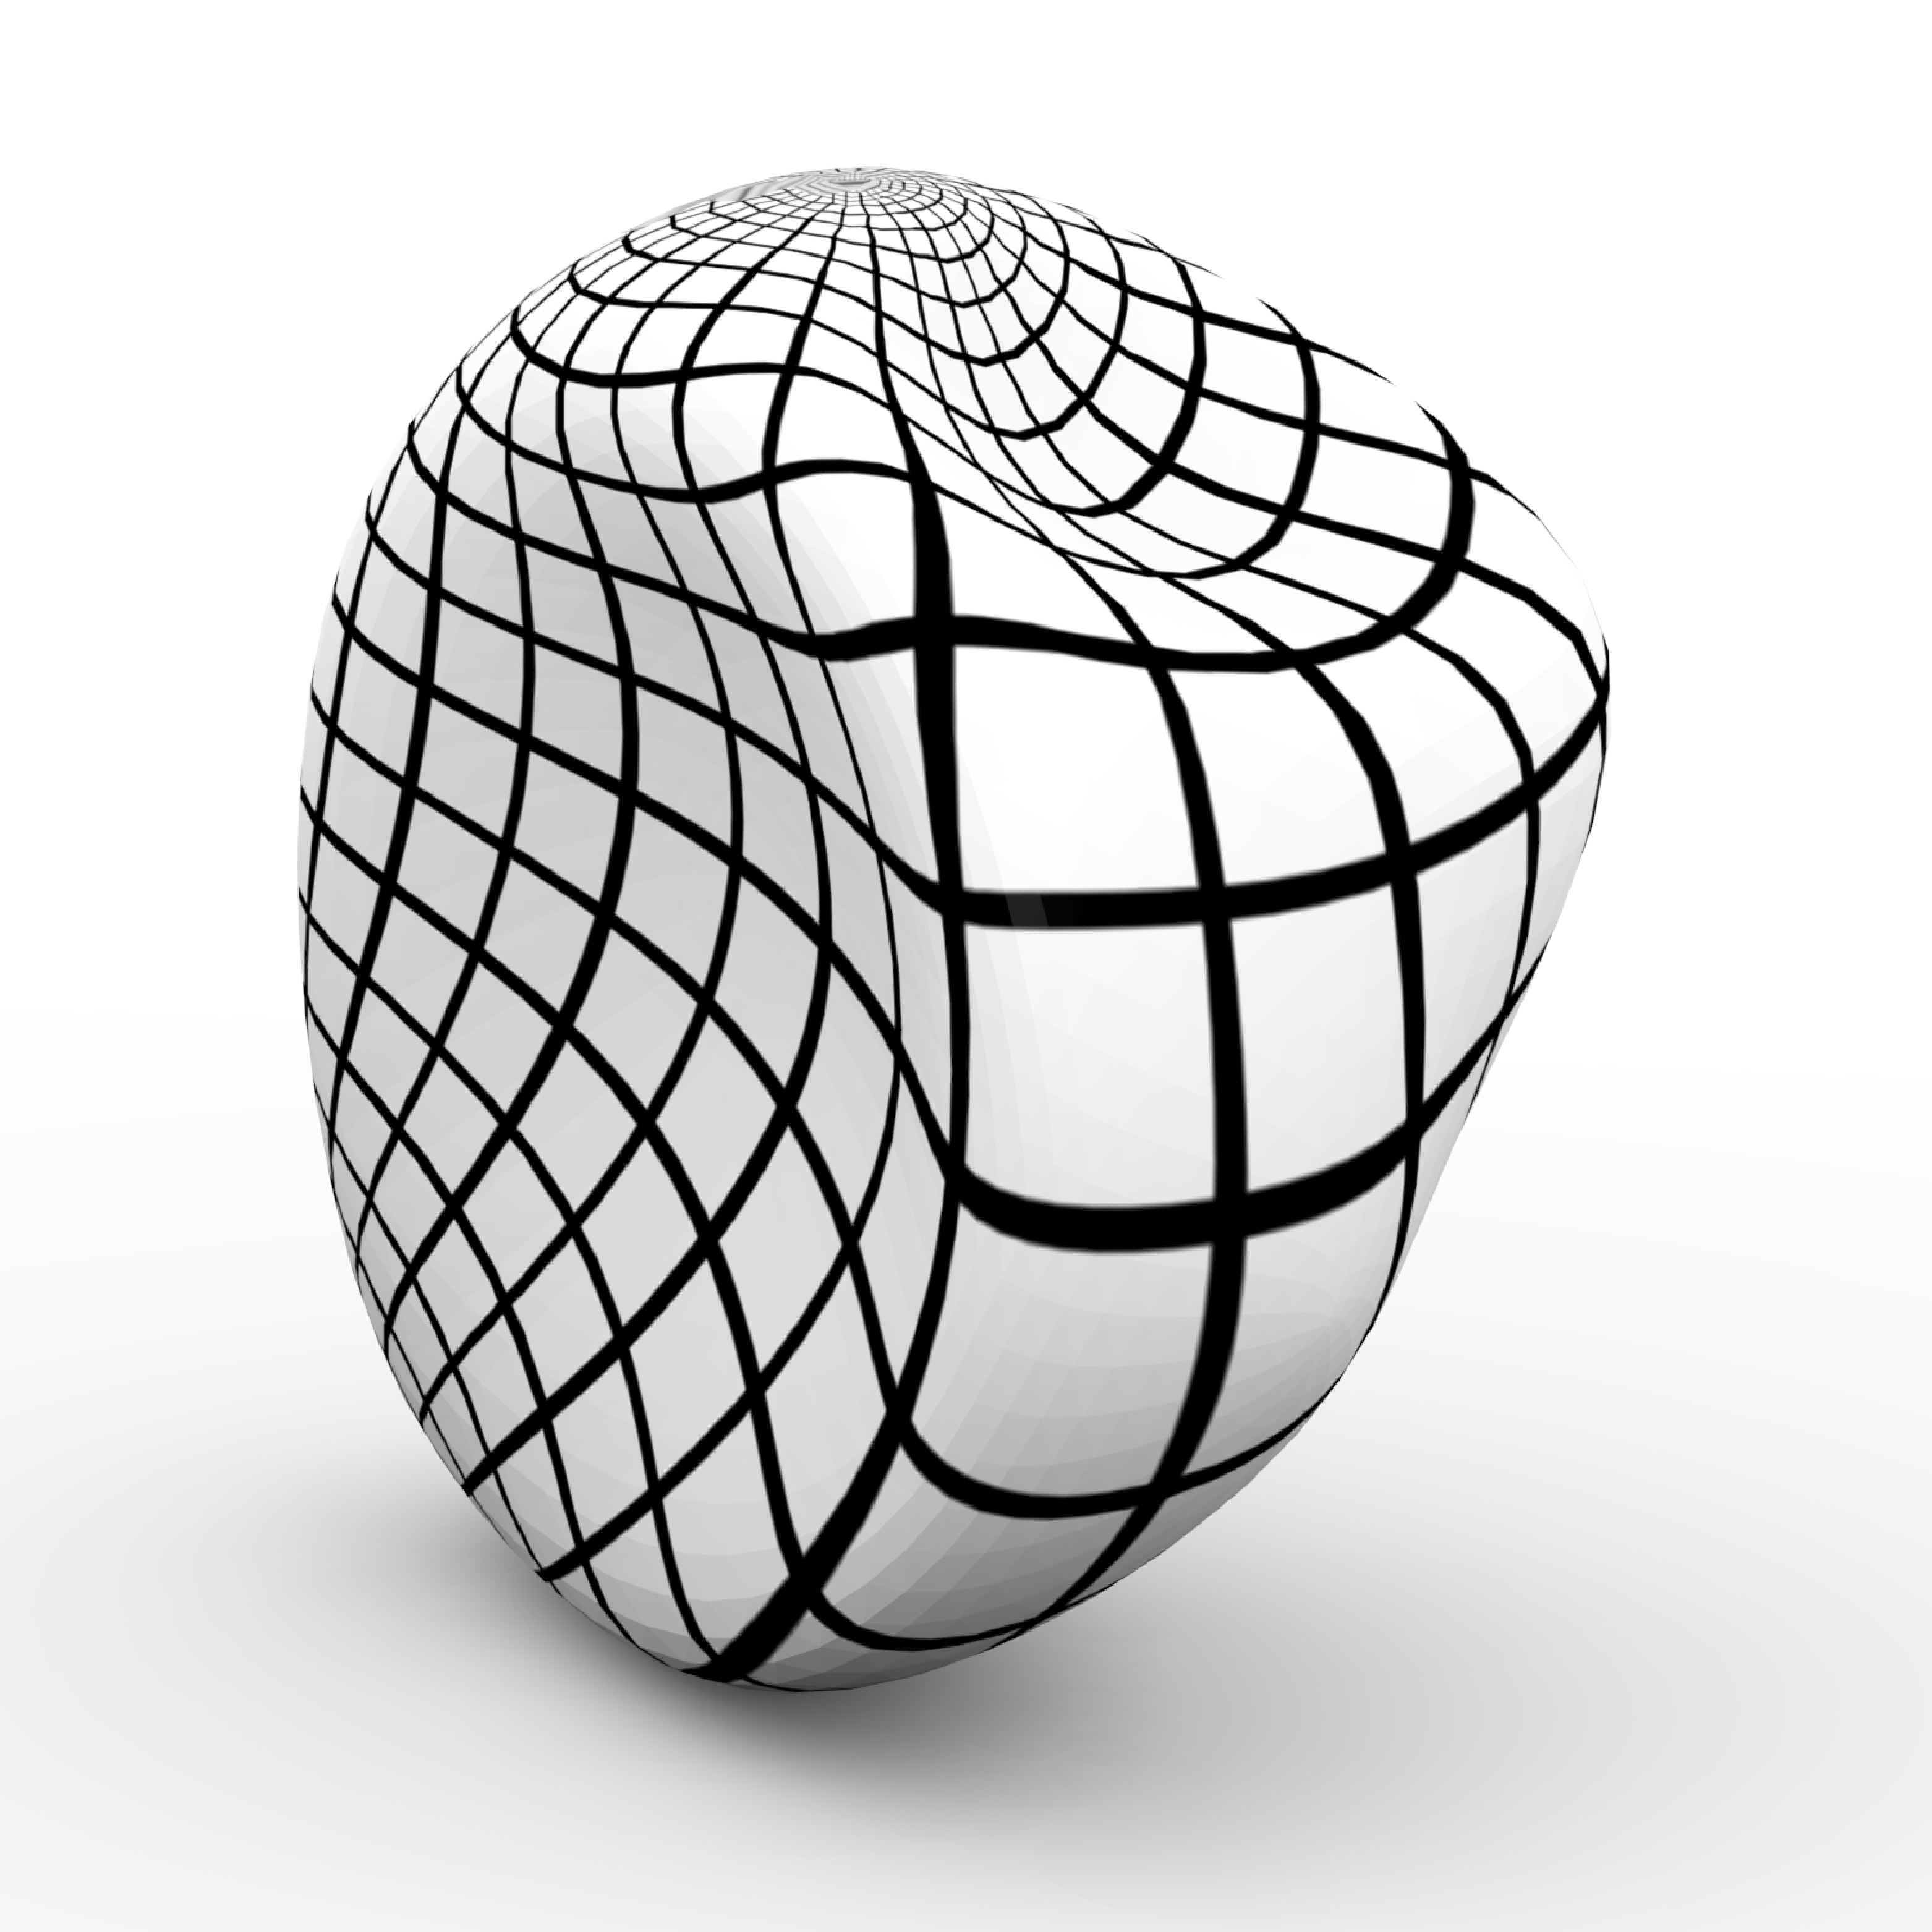
\includegraphics[height=5cm]{introduction/genus0_image.pdf}
\quad
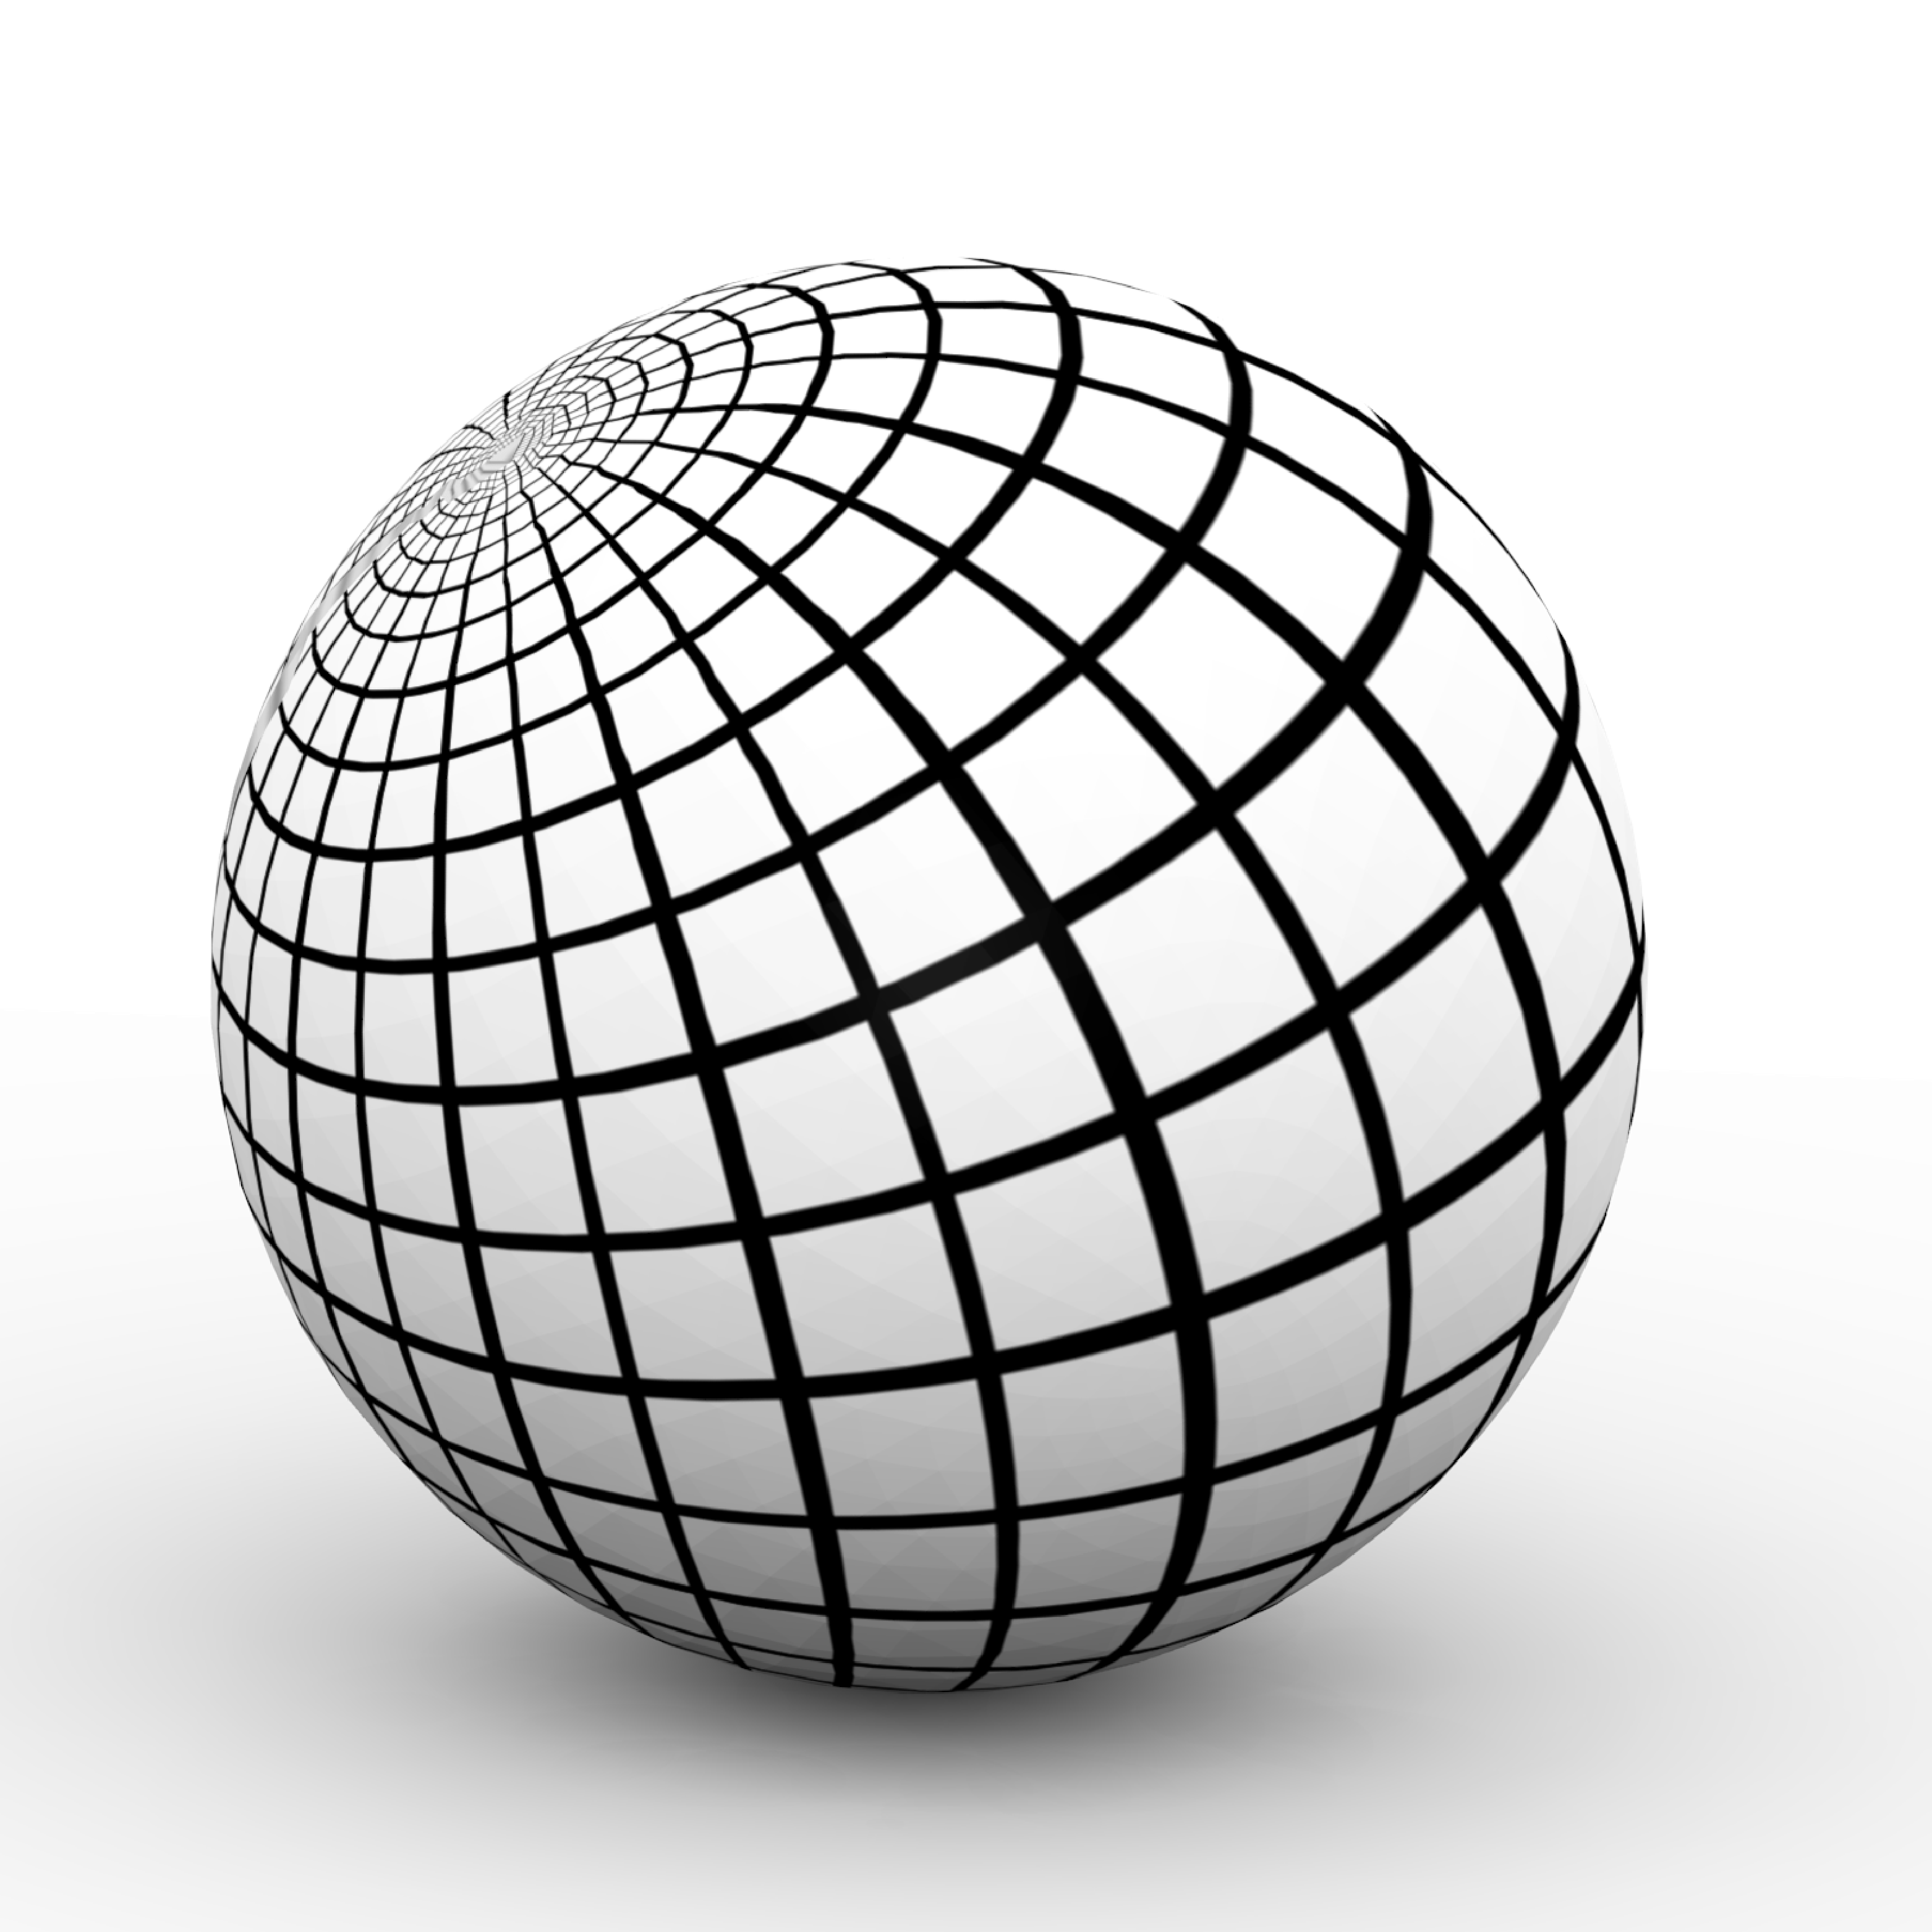
\includegraphics[height=5cm]{introduction/genus0_domain.pdf}
 }
\resizebox{0.8\linewidth}{!}{
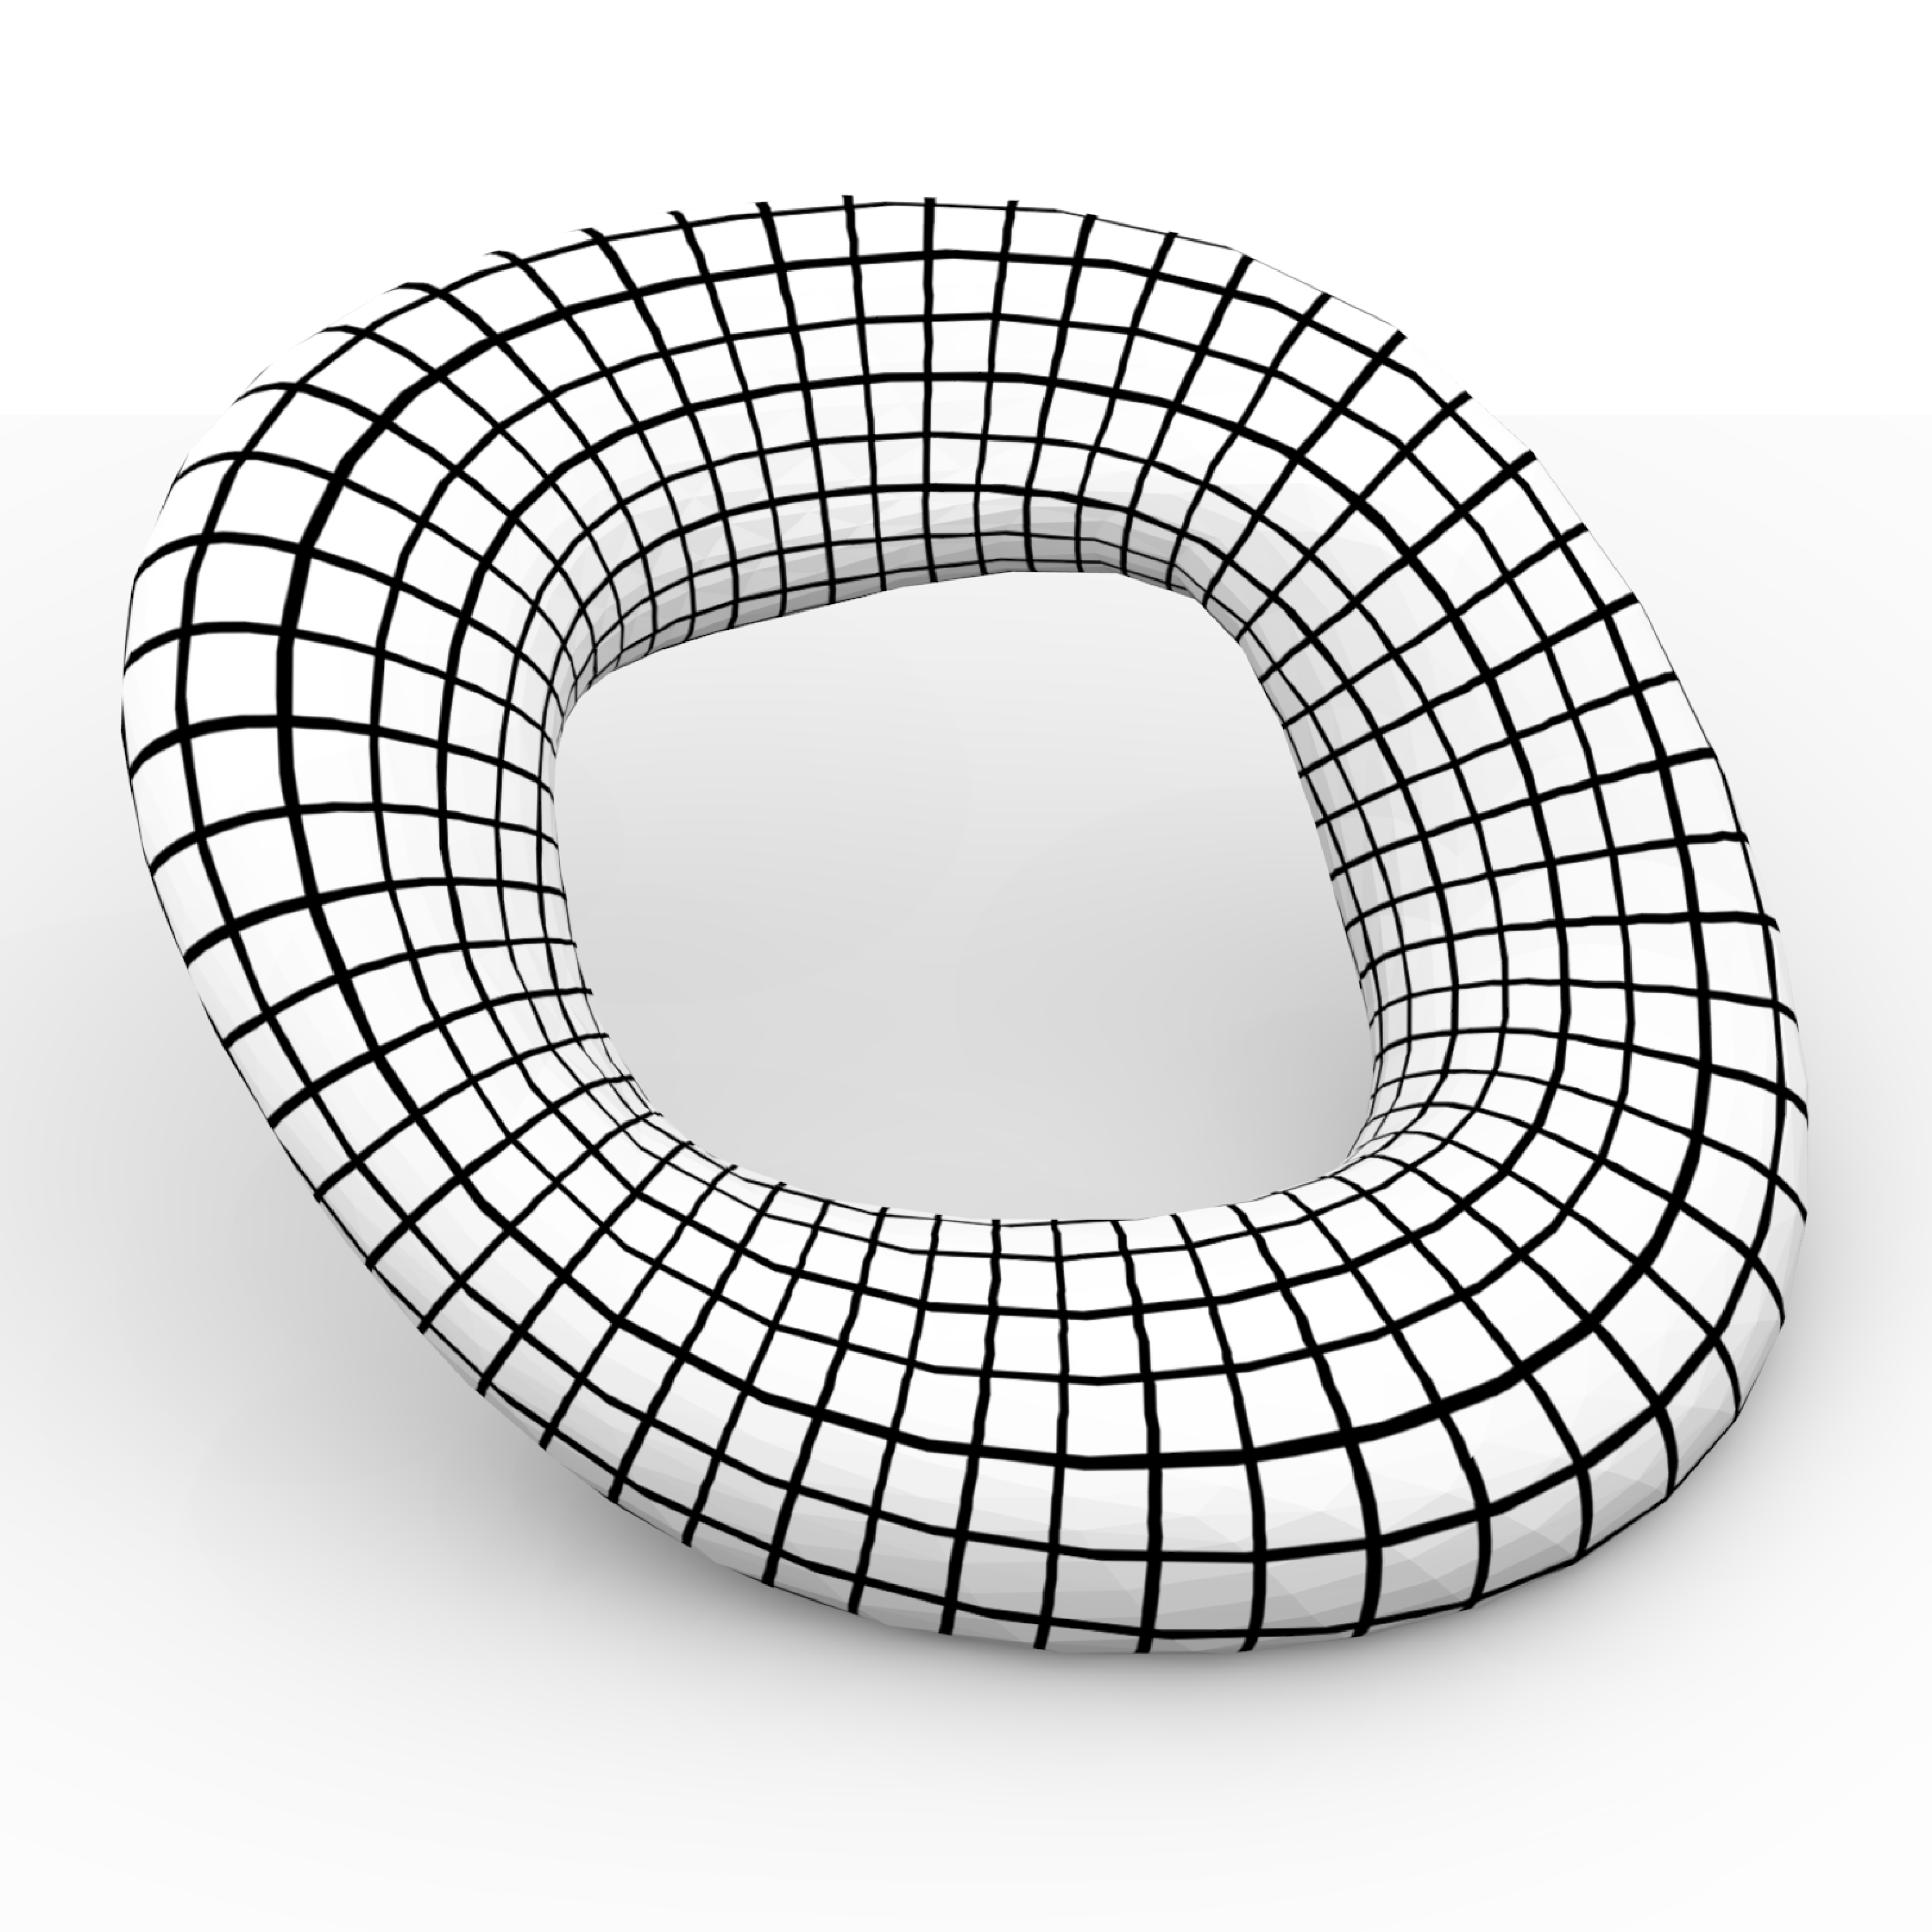
\includegraphics[height=5cm]{introduction/genus1_image.pdf}
\quad    
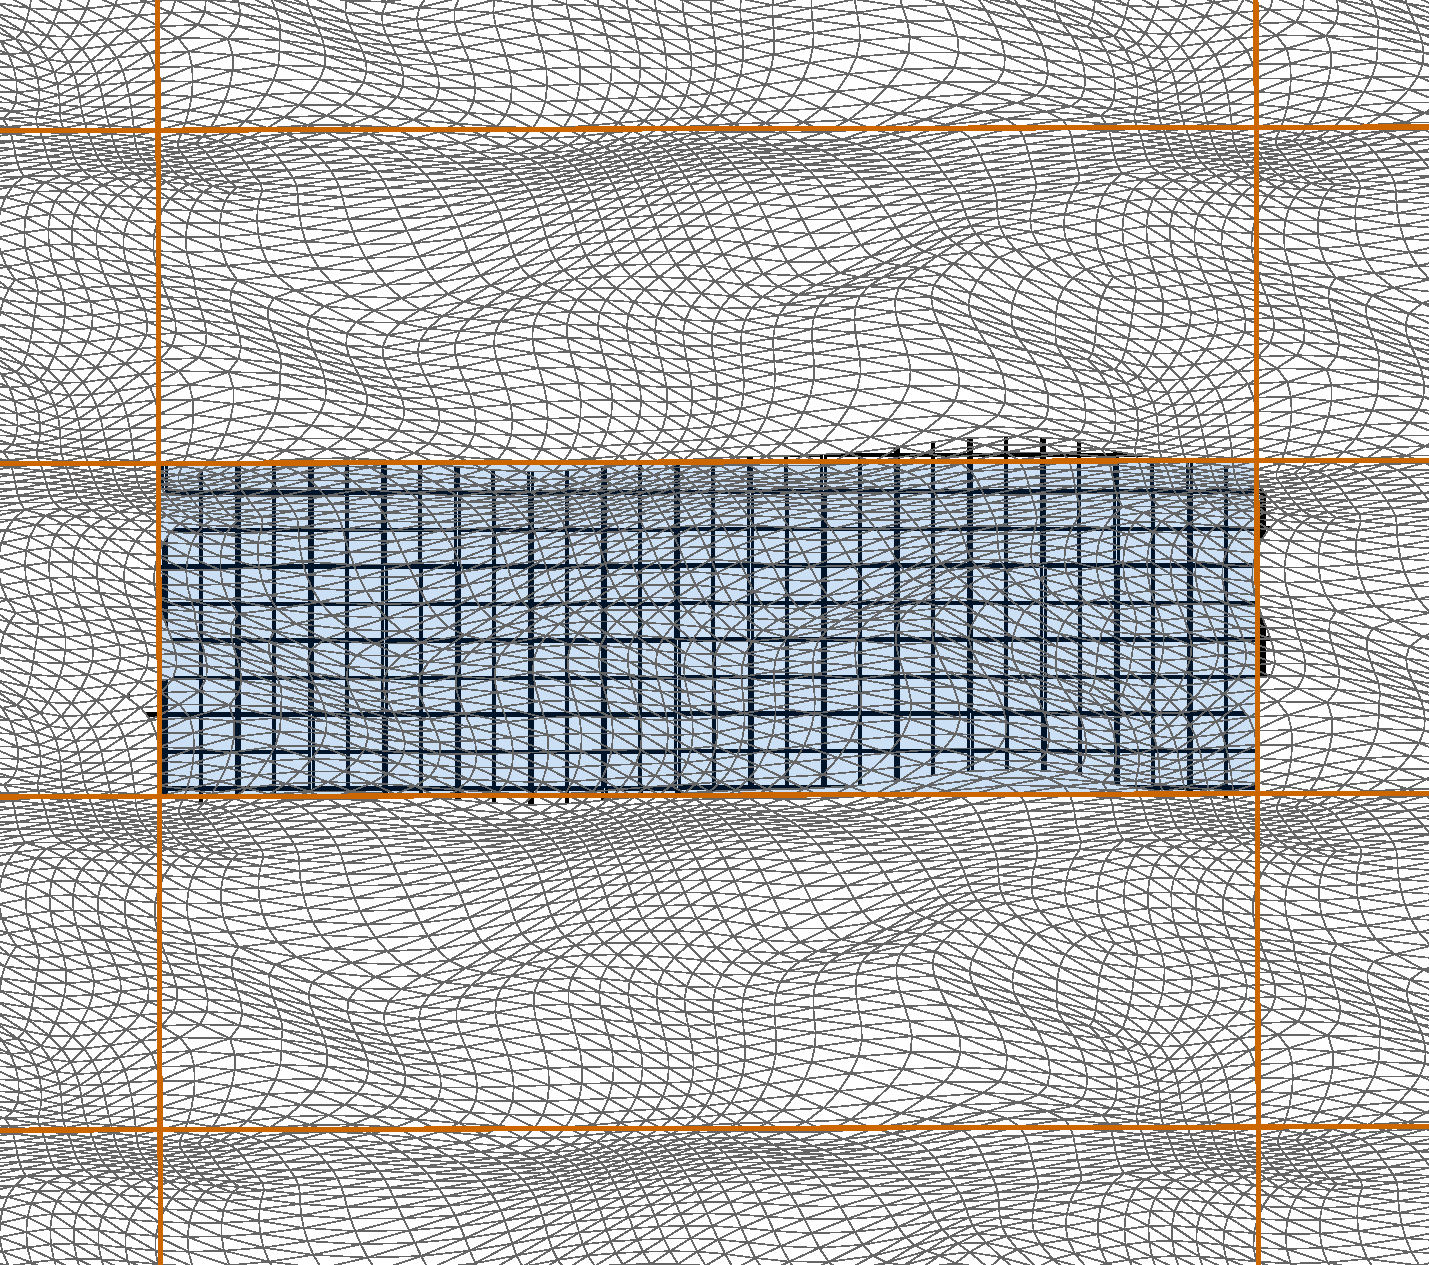
\includegraphics[height=4.8cm]{introduction/genus1_domain.pdf}
}
\resizebox{0.8\linewidth}{!}{
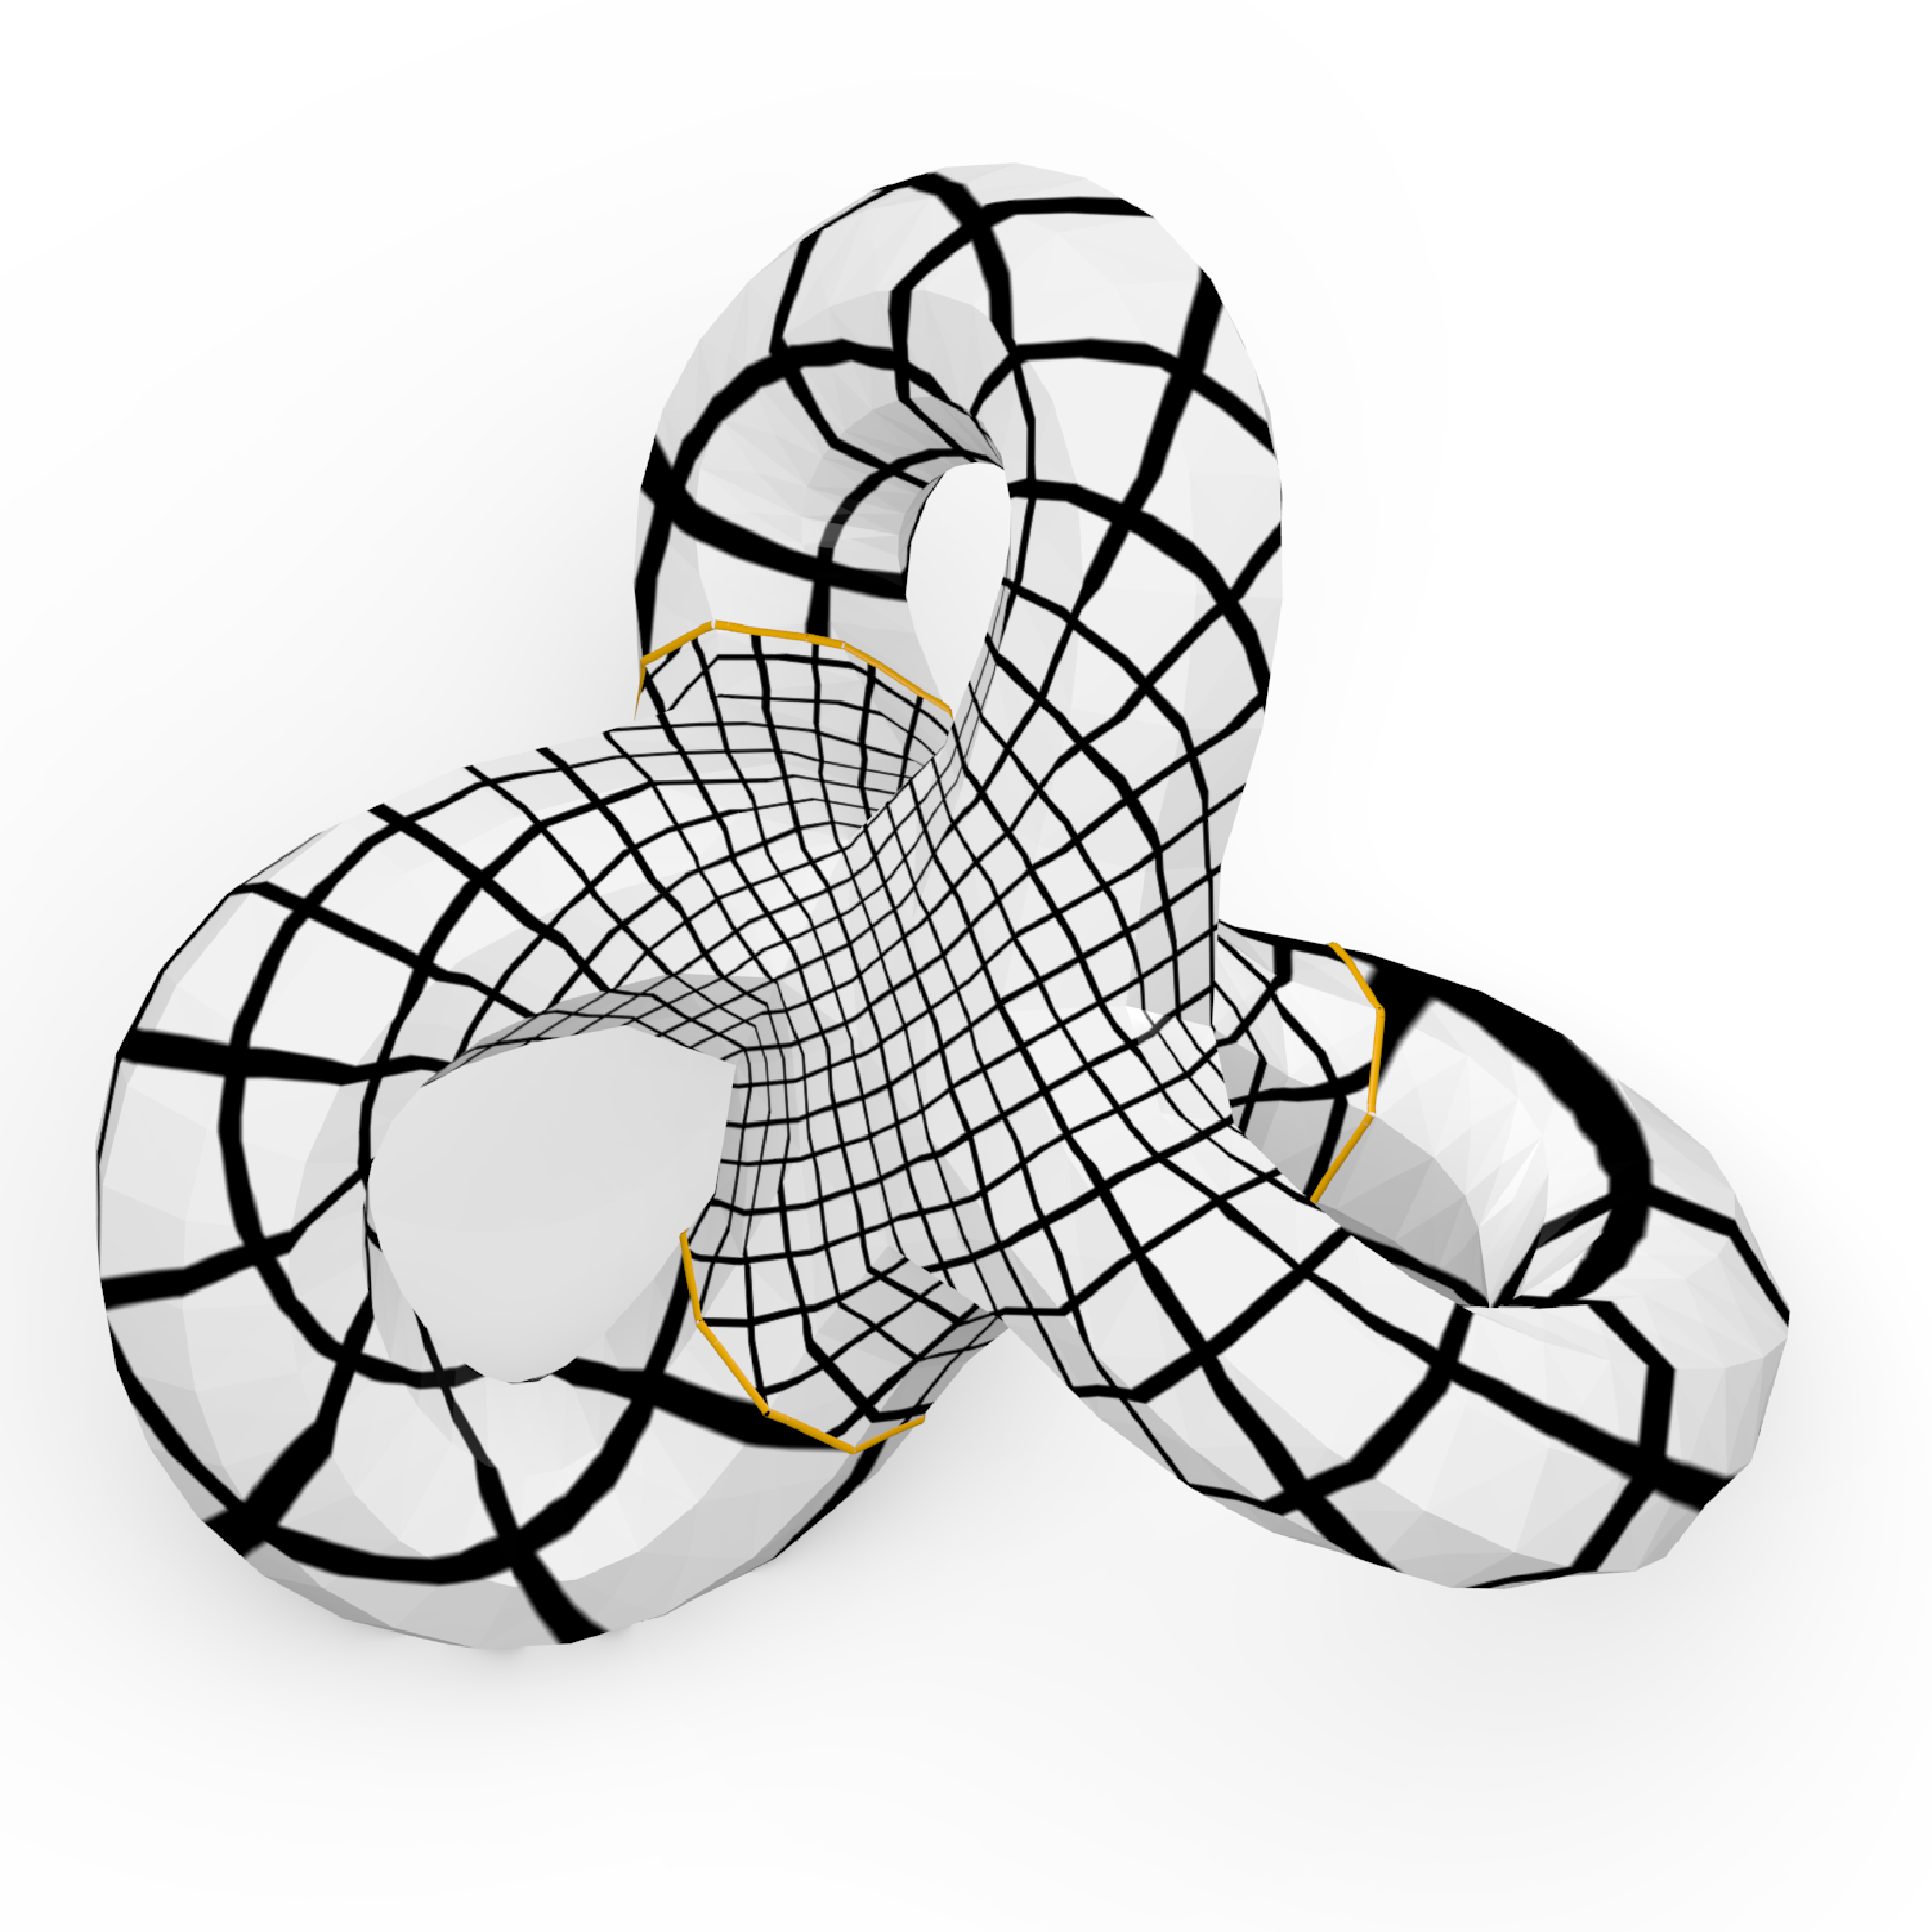
\includegraphics[height=5cm]{introduction/genus3_image.pdf}    
\quad   
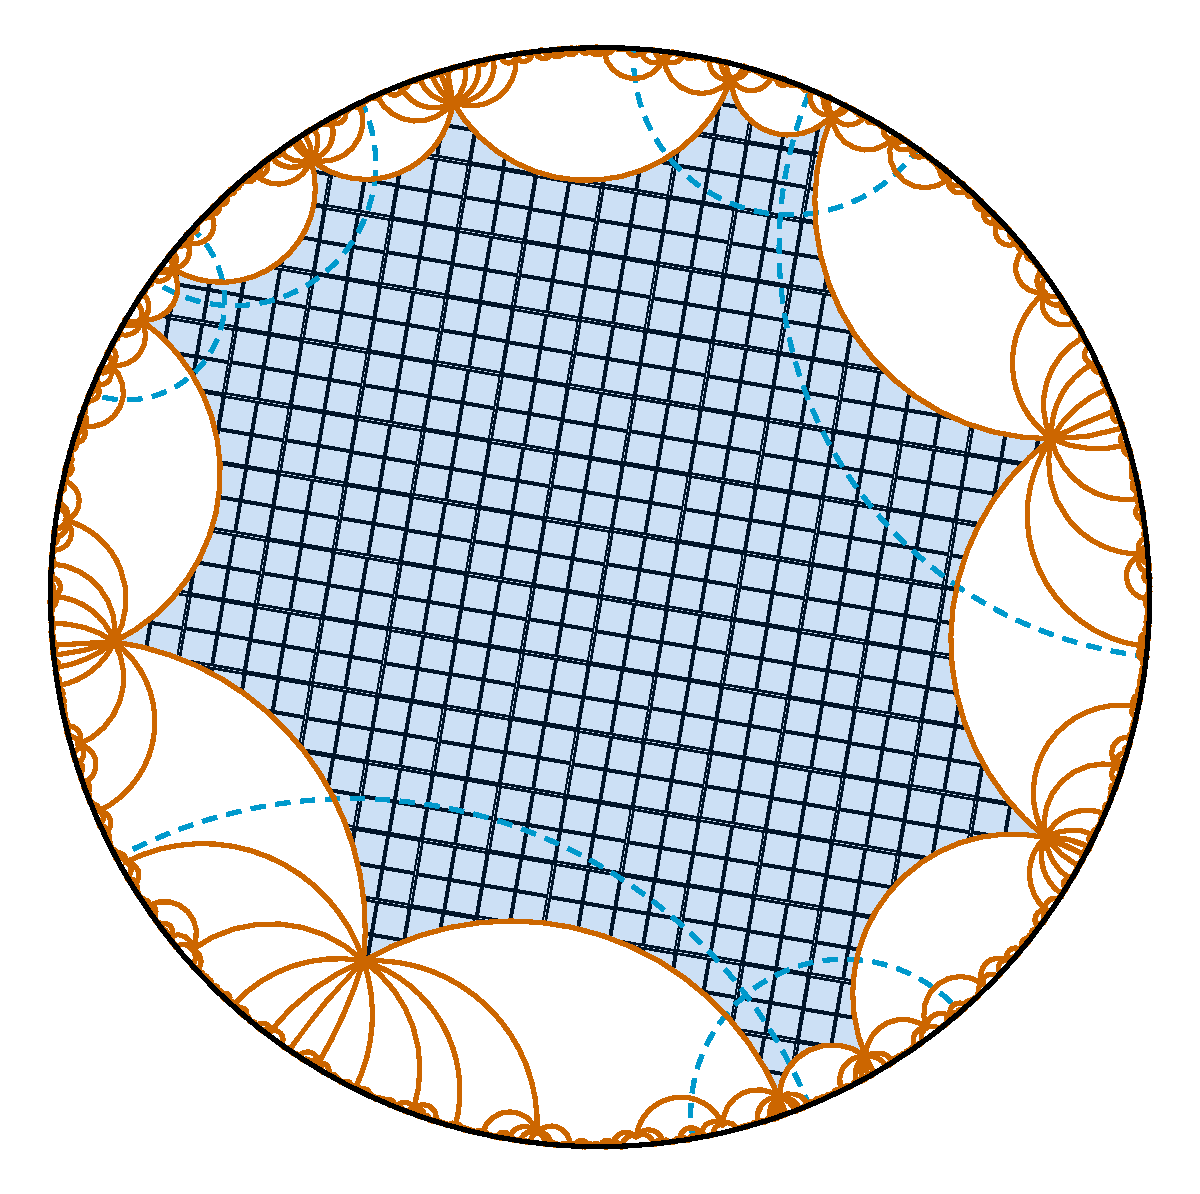
\includegraphics[height=5cm]{introduction/genus3_domain.pdf}
}
\setstretch{0.0}{\scriptsize\tt data/introduction/genus\{0/1/3\}\_data.xml} 
\caption{
Top: Uniformization of compact Riemann surfaces. 
The uniformization of topological spheres is treated in Section~\ref{sec:spheres}.
All spheres are conformally equivalent, we show a map to the round sphere. 
To visualize the conformality we map a grid by Mercator projection with non-standard poles.
Middle: Tori are covered in Section~\ref{sec:tori}.
Conformal tori can be parameterized over complex lattices. 
In this case the torus can be mapped to a rectangle lattice. 
We adjust the ratio of the the mapped grid to match the ratio of the rectangle in order to map the grid seamlessly onto the embedding.
Bottom: We describe uniformizations of surfaces of higher genus in Section~\ref{sec:higher_genus}.
The fundamental domain of the parameterization is a (canonical) hyperbolic polygon. 
It tessellates the hyperbolic plane by hyperbolic translations that generate the uniformizing group of the corresponding Riemann surface.
How to find a seamless grid pattern matching this domain is an open problem.
}
\label{fig:intro_uniformization}
\end{figure}

In this chapter we investigate various mathematical applications of discrete conformal maps. 
We build upon the work of Bobenko, Pinkall, and Springborn~\cite{Bobenko2010} and Springborn, Schr\"{o}der, and Pinkall~\cite{Springborn2008} for the euclidean case. We present examples for uniformizations of Riemann surfaces of genus $0$, $1$, and $g>1$ based on this theory, see Figure~\ref{fig:intro_uniformization}.

We generalize the setting in a way such that not only the scaling factors $u$ are variables of the functional but also the $\lambda$s itself can be varied. 
By this we can formulate the theory of conformally equivalent meshes on cyclic polyhedral surfaces. 
This was briefly noted in the previous work~\cite[p. 2211]{Bobenko2010}.
We state the euclidean, hyperbolic, and spherical variational principles together with the gradients and hessian matrices of the corresponding functional. 
As touched upon by Bobenko~\emph{et~al.} letting the $\lambda$s be variables we are able to create maps to regions bounded by circles~\cite[p. 2212]{Bobenko2010}.

This text is accompanied by a compact disk which contains the data for all of the examples presented in this part of the work. 
Where applicable we give the path to the data on the disk directly under the corresponding figure.
We describe the usage of the software and the XML data format that was used to create all the results in Chapter~\ref{chp:conformallab}.

%There is no existence, can be remedied using recent techniques developed by Luo et. al.~\cite{Luo13, Luo14}.
%Maybe reference Beardon and Stephenson~\cite{BS90}.

This chapter is organized as follows. We review the basic definitions of discrete conformal equivalence and conformal maps in Section~\ref{sec:basic_definitions}. Here we extend the notion of conformal equivalence to cyclic polyhedral surfaces.
In Section~\ref{sec:vari-princ} we state the variational principles for discrete conformal mappings to spherical, euclidean, and hyperbolic domains.
We give examples for discrete conformal maps between planar cyclic domains in Section~\ref{sec:planar_domains}. 
Among others we treat examples for cyclic circle domains and special multiply-connected domains.
Uniformizations of cyclic spheres are investigated in Section~\ref{sec:spheres}.
Section~\ref{sec:tori} is about the uniformization of Riemann surfaces of genus $1$.
We look into the convergence behavior of discrete conformal maps using discrete elliptic curves.
 Surfaces with genus $g>1$ are treated in Section~\ref{sec:higher_genus}.
 We describe how to construct Fuchsian uniformizations and the corresponding fundamental domains.
 The uniformization of hyperelliptic Riemann surfaces is a special case of the methods developed in the previous sections, see Section~\ref{sec:hyperelliptic}.
 

\section{Basic definitions}
\label{sec:basic_definitions}

\subsection{Cyclic polyhedral surfaces }

A \emph{euclidean polyhedral surface} is a surface obtained from
gluing euclidean polygons along their edges. (A \emph{surface} is a
two-dimensional manifold, possibly with boundary.)  In other words, a
euclidean polyhedral surface is a surface equipped with, first, an
intrinsic metric which is flat except at isolated points where it has
cone-like singularities, and, second, the structure of a CW complex
with geodesic edges. The set of vertices contains all cone-like
singularities. If the surface has a boundary, the boundary is
polygonal and the set of vertices contains all corners of the
boundary.

\emph{Hyperbolic polyhedral surfaces} and \emph{spherical polyhedral
surfaces} are defined analogously. They are glued from polygons in
the hyperbolic and elliptic planes, respectively. Their metric is
locally hyperbolic or elliptic, except at cone-like singularities.

We will only be concerned with polyhedral surfaces whose faces are all
cyclic, i.e., inscribed in circles. We call them \emph{cyclic
polyhedral surfaces}. More precisely, we require the polygons to be
cyclic before they are glued together. It is not required that the
circumcircles persist after gluing; they may be disturbed by cone-like
singularites. A polygon in the hyperbolic plane is considered cyclic
if it is inscribed in a curve of constant curvature. This may be a
circle (the locus of points at constant distance from its center), a
horocycle, or a curve at constant distance from a geodesic.

A \emph{triangulated surface}, or \emph{triangulation} for short, is a
polyhedral surface all of whose faces are triangles.  All
triangulations are cyclic.

\subsection{Notation}
\label{sec:notation}

\begin{figure}
\centering
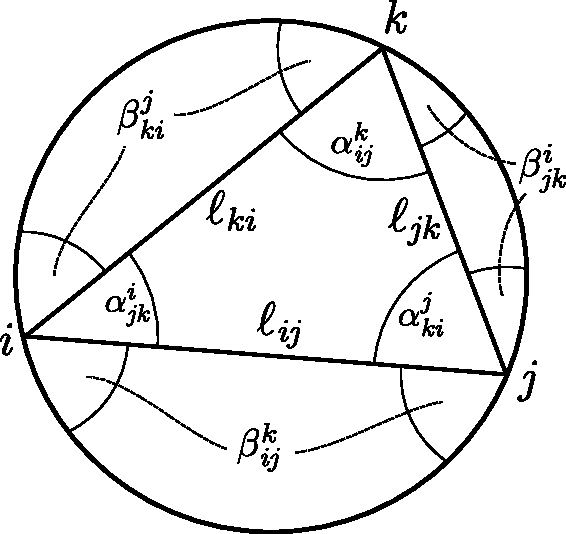
\includegraphics[width=0.4\textwidth]{notation_triangle_circle.pdf}
\caption{Notation of lengths and angles in a triangle $\it ijk \in F$.}
\label{fig:triangle_notation}	
\end{figure}

We will denote the sets of vertices, edges, and faces of a CW complex~$\Sigma$ by $V_{\Sigma}$, $E_{\Sigma}$, and $F_{\Sigma}$, and we will often omit the subscript when there is no danger of confusion.
For notational convenience, we require all CW complexes to be \emph{strongly regular}. 
This means that we require that faces are not glued to themselves along edges or at vertices, that two faces are not glued together along more than one edge or one vertex, and that edges have distinct end-points and two edges have at most one endpoint in common. 
This allows us to label edges and faces by their vertices. 
We will write $\mathit{ij}\in E$ for the edge with vertices $i,j\in V$ and $\mathit{ijkl}\in F$ for the face with vertices $i,j,k,l\in V$. 
We will always list the vertices of a face in the correct cyclic order, so that for example the face $\mathit{ijkl}$ has edges $\mathit{ij}$, $\mathit{jk}$, $\mathit{kl}$, and $\mathit{li}$.
The only reason for restricting our discussion to strongly regular CW complexes is to be able to use this simple notation. 
Everything we discuss applies also to general CW complexes.

In some formulas we need to iterate over directed edges. 
We denote the set of directed edges by $\vect{E}$. 
For each edge $\it ij\in E$ the set $\vect{E}$ contains two "half-edges" $\it ij\in \vect{E}$ and $\it ji \in \vect{E}$.
See also Chapter~\ref{chp:halfedge} for details on the implementation of a half-edge data structure.

For a triangle $\it ijk$ we denote the angle at vertex $i\in V$ as $\alpha^i_{\it jk}$. 
Further we define the angle $\beta^i_{\it ij}$ to be the angle between the tangent of the circum-circle of the triangle at $j$ or $k$ and the edge $\it jk$, see Figure~\ref{fig:triangle_notation}.
The angles $\beta$ are functions of $\alpha$. At the triangle $\it ijk$ it is
\begin{eqnarray*}
	2\cdot\beta_{\it jk}^i &=& \pi + \alpha_{\it jk}^i - \alpha_{\it ki}^j - \alpha_{\it ij}^k\\
	2\cdot\beta_{\it ki}^j &=& \pi - \alpha_{\it jk}^i + \alpha_{\it ki}^j - \alpha_{\it ij}^k\\
	2\cdot\beta_{\it ij}^k &=& \pi - \alpha_{\it jk}^i - \alpha_{\it ki}^j + \alpha_{\it ij}^k.
\end{eqnarray*}

\subsection{Discrete metrics}
\label{sec:discrete-metrics}

The \emph{discrete metric} of a euclidean (or hyperbolic or spherical) cyclic polyhedral surface $\Sigma$ is the function $\ell:E_{\Sigma}\rightarrow\R_{>0}$ that assigns to each edge $\it ij \in E_{\Sigma}$ its
length $\ell_{\it ij}$. 
It satisfies the polygon inequalities (one side is shorter than the sum of the others):
\begin{equation}
\label{eq:polygon_ineq}
% \forall i_{1}i_{2}\ldots i_{n}\in F_{\Sigma}:
% \quad
\left.
\quad
\begin{aligned}
-\ell_{i_{1}i_{2}}+\ell_{i_{2}i_{3}}+&\ldots+\ell_{i_{n-1}i_{n}}
>0\\
\ell_{i_{1}i_{2}}-\ell_{i_{2}i_{3}}+&\ldots+\ell_{i_{n-1}i_{n}}
>0\\
&\vdots\\
\ell_{i_{1}i_{2}}+\ell_{i_{2}i_{3}}+&\ldots-\ell_{i_{n-1}i_{n}}
>0
\end{aligned}
\quad
\right\}
\quad
\text{for all $i_{1}i_{2}\ldots i_{n}\in F_{\Sigma}$}
\end{equation}

In euclidean and hyperbolic geometry, the polygon inequalities are sufficient for the existence of a polygon with given edge lengths. 
Furthermore, a \emph{cyclic} polygon is uniquely determined by its edge lengths. 
Thus, the discrete metric determines the geometry of a cyclic polyhedral surface~\cite{KSS15}:

If $\Sigma$ is a surface with the structure of a CW~complex and a function $\ell:E_{\Sigma}\rightarrow\R_{>0}$ satisfies the polygon inequalities~\eqref{eq:polygon_ineq}, then there is a unique euclidean
cyclic polyhedral surface (and also a unique hyperbolic cyclic polyhedral surface) with CW~complex~$\Sigma$ and discrete metric~$\ell$.

The edge lengths of a cyclic polygon in the sphere satisfy another independent inequality: The perimeter is less than $2\pi$.  
The discrete metric of a spherical cyclic polyhedral surface satisfies the additional inequalities
\begin{equation}
\label{eq:spherical_polygon_ineq}
\ell_{i_{1}i_{2}}+\ell_{i_{2}i_{3}}+\ldots+\ell_{i_{n-1}i_{n}}<2\pi
\quad
\text{for all $i_{1}i_{2}\ldots i_{n}\in F_{\Sigma}$.}
\end{equation}
Given a function $\ell:E_{\Sigma}\rightarrow\R_{>0}$ satisfying the inequalities~\eqref{eq:polygon_ineq}
and~\eqref{eq:spherical_polygon_ineq}, then there is a unique cyclic spherical polyhedral surface with discrete metric $\ell$.

\subsection{Discrete conformal equivalence}
\label{sec:discr-conf-equiv}

\begin{figure}
\centering
\resizebox{0.6\textwidth}{!}{
\input{figures/spherical.pdf_t}
\input{figures/hyperbolic.pdf_t}
}
\caption{
Relations between euclidean edge lengths $l$ and conformally equivalent spherical (left) and hyperbolic (right) lengths $\tilde l$ respectively. 
For the spherical case we have $\sin\Big(\frac{\ellt}{2}\Big)=\frac{\ell}{2}$ and for the hyperbolic case it is $\sinh\Big(\frac{\ellt}{2}\Big)=\frac{\ell}{2}$.
}
\label{fig:geometries}
\end{figure}


We define discrete conformal equivalence for cyclic polyhedral surfaces that are combinatorially equivalent. Thus, we may assume that the surfaces share the same CW complex $\Sigma$ equipped with different metrics.

Two \emph{euclidean} cyclic polyhedral surfaces with discrete metrics $\ell,\tilde\ell:E_{\Sigma}\rightarrow\R_{>0}$ are \emph{discretely conformally equivalent} if there exists a function $u:V_{\Sigma}\rightarrow\R$ such that
\begin{equation}
\label{eq:tilde_ell_euc}
\tilde\ell_\mathit{ij}=e^{\frac{1}{2}(u_{i}+u_{j})}\ell_\mathit{ij}.
\end{equation}

Two \emph{hyperbolic} cyclic polyhedral surfaces with discrete metrics $\ell,\tilde\ell:E_{\Sigma}\rightarrow\R_{>0}$ are \emph{discretely conformally equivalent} if there exists a function $u:V_{\Sigma}\rightarrow\R$ such that
\begin{equation}
\label{eq:tilde_ell_hyp}
\sinh\Big(\frac{\tilde\ell_\mathit{ij}}{2}\Big)
= e^{\frac{1}{2}(u_{i}+u_{j})}\,
\sinh\Big(\frac{\ell_\mathit{ij}}{2}\Big).
\end{equation}


Two \emph{spherical} cyclic polyhedral surfaces with discrete metrics $\ell,\tilde\ell:E_{\Sigma}\rightarrow\R_{>0}$ are \emph{discretely conformally equivalent} if there exists a function $u:V_{\Sigma}\rightarrow\R$ such that
\begin{equation}
\label{eq:tilde_ell_sph}
\sin\Big(\frac{\tilde\ell_\mathit{ij}}{2}\Big)
= e^{\frac{1}{2}(u_{i}+u_{j})}\,
\sin\Big(\frac{\ell_\mathit{ij}}{2}\Big).
\end{equation}

We will also consider ``mixed versions'': For example, a cyclic euclidean polyhedral surface with discrete metric $\ell:E_{\Sigma}\rightarrow\R_{>0}$ and a cyclic hyperbolic polyhedral surface with discrete metric $\tilde\ell:E_{\Sigma}\rightarrow\R_{>0}$ are discretely conformally equivalent if
\begin{equation*}
\sinh\Big(\frac{\tilde\ell_\mathit{ij}}{2}\Big)
= e^{\frac{1}{2}(u_{i}+u_{j})}\ell_\mathit{ij}.
\end{equation*}

Analogously the spherical version for a spherical metric $\tilde\ell:E_{\Sigma}\rightarrow\R_{>0}$ reads
\begin{equation*}
\sin\Big(\frac{\tilde\ell_\mathit{ij}}{2}\Big)
= e^{\frac{1}{2}(u_{i}+u_{j})}\ell_\mathit{ij},
\end{equation*}
see also Figure~\ref{fig:geometries}. 

\subsection{Triangulations: Characterization by length cross-ratios}
\label{sec:cross-ratios}

For triangulations we have an alternative characterization of conformal equivalence in terms of length cross-ratios. For two adjacent triangles $\it ijk\in F$ and $\it jil\in F$ the length cross-ratio of the common edge $\it ij\in E$ is defined as
\begin{equation}
\lcr_{\it ij}\vcentcolon=\frac{\ell_{\it il}\ell_{\it jk}}{\ell_{\it lj}\ell_{\it ki}}.
\end{equation}

\begin{proposition}
Two euclidean triangulations $(\Sigma, \ell)$ and $(\Sigma, \tilde \ell)$ are discretely conformally equivalent if and only if for each interior edge $\it ij\in E$, the induced length cross-ratios agree.
\end{proposition}

In addition to this characterization we can recover a representative metric from the length cross-ratios.
The length cross-ratios satisfy the product equation at each vertex $i\in V$
\begin{equation}
\prod_{\it ij\ni i} \lcr_{\it ij} = 1.
\end{equation}
Define values attached to angles of the triangulation, e.g., 
\begin{equation}
c^i_{\it jk}=\frac{\ell_{\it jk}}{\ell_{\it ij}\ell_{\it ki}}\label{eq:angle_parameter}
\end{equation} 
is attached to angle at vertex $i$ of the triangle $\it ijk\in F$.
With this parameter the length cross-ratios can we written as
\begin{equation}
\lcr_{\it ij}=\frac{c^i_{\it jk}}{c^i_{\it lj}}.
\end{equation}
for a given function $\lcr$ defined on edges of the triangulation we can find parameters $c$ on angles that satisfy Equation~\ref{eq:angle_parameter} by choosing one of the $c$ at each vertex.
The corresponding metric $\ell$ is then given by the relations
\begin{equation}
\ell_{\it ij} = \frac{1}{\sqrt{c^i_{\it jk}c^j_{\it ki}}} = \frac{1}{\sqrt{c^i_{\it lj}c^j_{\it il}}}.
\end{equation} 

What is now the generalization of this concept to cyclic polyhedral surfaces?

\subsection{Quadrangulations: Characterization by cross-ratios and Hirota systems}

\subsection{Even cycles: Characterization by length multi-ratios}

\begin{itemize}
\item even polygons
\item even cycles
\end{itemize}

Note: Even polygons and quadrangulation of the disk.


Until now we have only talked about discrete conformal equivalence of discrete euclidean/spherical/hyperbolic metrics.
We now turn to discrete conformal mappings between discrete cyclic polyhedral surfaces.

\subsection{Discrete conformal maps}

Let $\Sigma$ be a cyclic polyhedral surface. Define a derived cyclic polyhedral
surface $\tilde \Sigma$ by triangulating all faces with more than three vertices. The way of triangulation
is arbitrary. Let $E_0$ be the set of original edges and let $E_1$ be the set of new edges
in the triangulation, i.e., $E=E_0\cup E_1$.

\begin{problem}[prescribed angle sums]
\label{prob:total_angles}
\textbf{\itshape{Given}}
\begin{compactitem}
\item the discrete metric $\ell:E\rightarrow\R_{>0}$ of a euclidean cyclic polyhedral surface,
\item a desired total angle $\Theta_{i}>0$ for each vertex $i\in V$,
\end{compactitem}
\smallskip\noindent%
\textbf{\itshape{find}} the discrete metric $\tilde\ell:E\rightarrow\R_{>0}$ of a discretely conformally equivalent euclidean/hyperbolic/spherical cyclic polyhedral surface that has the desired total angle $\Theta_{i}$ around each vertex $i\in V$.
\end{problem}

For interior vertices, $\Theta_i$ denotes a desired cone angle. 
For boundary vertices, $\Theta_i$ denotes a desired interior angle of the polygonal boundary. 
If $\Theta_{i}=2\pi$ for all interior vertices, then Problem~\ref{prob:total_angles} asks for a flat metric in the discrete conformal class (with prescribed boundary angles if the surface has a boundary). 
Note that the solution of this problem is a discretely conformally equivalent metric only on $E_0$ and for the original complex $\Sigma$.

We also consider the more general mapping problem. 
\begin{problem}[prescribed scale factors and angle sums]
\label{prob:factors_and_angles}
\textbf{\itshape{Given}}
\begin{compactitem}
\item the discrete metric $\ell:E\rightarrow\R_{>0}$ of a euclidean cyclic polyhedral surface,
\item a partition $V=V_0\cup V_1$ of the vertex set
\item a prescribed logarithmic scale factor $u_i\in \R$ for each vertex $i\in V_0$
\item a prescribed angle $\Theta_{i} > 0$ for each vertex $i\in V_1$,
\end{compactitem}
\smallskip\noindent%
\textbf{\itshape{find}} the discrete metric $\tilde\ell:E\rightarrow\R_{>0}$ of a discretely conformally equivalent euclidean/hyperbolic/spherical cyclic polyhedral surface that has the desired total angles $\Theta_{i}$ around each vertex $i\in V_1$.
\end{problem}

Solving these problems amounts to the solution of a system of non-linear equations in terms of $u_i$ for $i\in V$ and $\lambda_{\it ij}$ for $\it ij \in E_1$:

\begin{align}
	\Theta_i &=\sum_{\it ijk \ni i}\alphat_{\it ji}^i & i\in V\label{eq:vertex_system}\\
	0 &= (\alphat_{\it ij}^k + \alphat_{\it ij}^l) - (\alphat^i_{\it jl} + \alphat^i_{\it kj}) - (\alphat^j_{\it ki} + \alphat^j_{\it il}) & \textit{ij} \in E_1\label{eq:edge_system}
\end{align}

The angle $\alphat_{\it ji}^i$ is the new angle at vertex $i$ in the triangle $\it ijk\in F$, see Figure~\ref{fig:triangle_notation}.
It is a function of the new edges lengths $\tilde\ell_{\it ij}$.
Equation~\ref{eq:vertex_system} is the condition for the angles around each vertex $i \in V$ to sum up to a prescribed $\Theta_i$.
Condition~\ref{eq:edge_system} is satisfied if and only if the quadrilateral $\it ijkl\in \Sigma$ consisting of triangles $\it ijk\in \tilde \Sigma$ and $\it jil\in \tilde \Sigma$ is inscribed in a circle. Note that this condition is valid in all geometries. For the euclidean case the condition reduces to $\pi=\alphat_{\it ij}^k + \alphat_{\it ij}^l$.

\section{Variational principles for discrete conformal maps}
\label{sec:vari-princ}

\begin{definition}
Let $\ell_{\it ij}:E\to R_{>0}$ be the edge lengths of $\tilde \Sigma$ and $u:V_{\tilde\Sigma}\rightarrow\R$. Define
\begin{eqnarray*}
\lambda_{\it ij} &\vcentcolon=& 2\log \ell_{\it ij}\label{eq:lambda_def}\\
\tilde\lambda_{\it ij} &\vcentcolon=& \lambda_{\it ij}+u_i+u_j\\
\tilde \ell_{\it ij} &\vcentcolon=& e^{\frac{1}{2}\tilde \lambda_{\it ij}}=e^{\frac{1}{2}(u_i + u_j)}\ell_{\it ij}
\end{eqnarray*}
\end{definition}
In the latter we denote angles that are functions of new lengths $\ellt$ with tilde marks, e.g., $\alphat_{\it jk}^i$.

We consider three functionals defined on the triangulation $\tilde \Sigma$:
\begin{eqnarray*}
	E^{\rm euc}(\lambda,u) &\to& \R\\
	E^{\rm hyp}(\lambda,u) &\to& \R\\
	E^{\rm sph}(\lambda,u) &\to& \R.
\end{eqnarray*}
By $\lambda, u$ we mean the vector of all $\lambda_{\it ij}$ for $\it ij \in E_1$ and $u_i$ for all $i\in V$, i.e., $(\lambda, u)\in \R^{\# E_1}\times\R^{\#V}$.
We treat all $u_i$ with $i\in V$ and all $\lambda_{\it ij}$ $\ij \in E_1$ as free variables. The values for $\lambda_{\it ij}$ with $\it ij\in E_0$ are fixed and are given by Equation~\ref{eq:lambda_def}. By allowing the $\lambda$s in $E_1$ to be variable the critical point of each of the functionals has a circular quadrilateral at each edge $\it ij\in E_1$, see, e.g., Equation~\ref{eq:lambda_deriv_euc}.

The functionals can be defined generically as
\begin{definition}{Generic functional}
\begin{eqnarray}
	E(\lambda, u) &\vcentcolon=& \sum_{\it ijk\in F}\left(f_{\it ijk}(\tilde\lambda) - \frac{\pi}{2}\left(\tilde \lambda_{jk} + \tilde \lambda_{ki} + \tilde \lambda_{ij}\right)\right) + \sum_{i\in V} \Theta_i u_i.
\end{eqnarray}
\end{definition}

The function $f_{\it ijk}$ is defined as
\begin{eqnarray}
f_{\it ijk}(\lambda) &\vcentcolon=&\beta_{\it jk}^i \lambda_{jk} + \beta_{\it ki}^j \lambda_{ki} + \beta_{\it ij}^k \lambda_{ij}\\ 		
&&+\ML(\alpha_{\it jk}^i) + \ML(\alpha_{\it ki}^j) + \ML(\alpha_{\it ij}^k) + \ML(\beta_{\it jk}^i) + \ML(\beta_{\it ki}^j) + \ML(\beta_{\it ij}^k)\nonumber\\
&&+\ML\left(\frac{1}{2}\left(\pi - \alpha_{\it jk}^i - \alpha_{\it ki}^j - \alpha_{\it ij}^k\right)\right).\nonumber
\end{eqnarray}
See Section~\ref{sec:notation} for the definition of the angles $\alpha$ and $\beta$. 
The triangle angles $\alpha$ are functions of the lengths $\ell$ and are different for each of the geometries. 
Thus $f$ is different for each of the geometries.
Note that using $\alpha_{\it jk}^i + \alpha_{\it ki}^j + \alpha_{\it ij}^k = \pi$ for $\it ijk \in F$ in the euclidean case we get a simplified version of the functional. It is
\begin{eqnarray*}
f^{\rm euc}_{\it ijk}(\lambda) &=& \alpha_{\it jk}^i \lambda_{jk} + \alpha_{\it ki}^j \lambda_{ki} + \alpha_{\it ij}^k \lambda_{ij} + 2\ML(\alpha_{\it jk}^i) + 2\ML(\alpha_{\it ki}^j) + 2\ML(\alpha_{\it ij}^k).
\end{eqnarray*}

\begin{proposition}{Partial derivatives of $f_{\it ijk}$}
\begin{equation}
\frac{\partial f_{\it ijk}}{\partial \lambda_{\it ij}}=\alpha^k_{\it ij},\quad\quad
\frac{\partial f_{\it ijk}}{\partial \lambda_{\it jk}}=\alpha^i_{\it jk},\quad\quad
\frac{\partial f_{\it ijk}}{\partial \lambda_{\it ki}}=\alpha^j_{\it ki}.
\end{equation}
\end{proposition}

The partial derivatives of $E$ are
\begin{eqnarray}
	\frac{\partial E}{\partial u_i} &=& \Theta_i - \sum_{\it ijk\ni i}\alphat_{\it jk}^i \\
	\frac{\partial E}{\partial \lambda_{\it ij}} &=& \frac{1}{2}\left((\alphat_{\it ij}^k + \alphat_{\it ij}^l) - (\alphat^i_{\it jl} + \alphat^i_{\it kj}) - (\alphat^j_{\it ki} + \alphat^j_{\it il})\right).\label{eq:lambda_deriv_generic}
\end{eqnarray}
In the second term the angles $\alphat_{\it ij}^k$ and $\alphat_{\it ji}^l$ are the angles opposite to the edge $\it ij\in E$ in the 
triangles on both sides of the edge. Note that in the euclidean case Equation~\ref{eq:lambda_deriv_generic} reduces to
\begin{eqnarray}
	\frac{\partial E^{\rm euc}}{\partial \lambda_{\it ij}} &=& \alphat_{\it ij}^k + \alphat_{\it ji}^l - \pi.\label{eq:lambda_deriv_euc}
\end{eqnarray}

We give formulas for $\alphat$ and derive the Hessian matrices for the functionals in each of the three cases.

\subsection{Euclidean version}
\label{sec:euclidean_fuctional}

Let $\alphat^i_{\it jk}$ be the angle opposite to edge $\it jk$ in the triangle $\it ijk\in F$ with edge lengths $\ell_{\it ij}$, $\ell_{\it jk}$, and $\ell_{\it ki}$. In euclidean geometry we calculate $\alphat^i_{\it jk}$ using the half-angle formula
\[\tan\Big(\frac{ \alpha_{\it jk}^i}{2}\Big) = \sqrt{\frac
{(-\ell_{\it ij} +\ell_{\it jk} +\ell_{\it ki})(\ell_{\it ij} +\ell_{\it jk} -\ell_{\it ki})}
{(\ell_{\it ij} -\ell_{\it jk} +\ell_{\it ki})(\ell_{\it ij} + \ell_{\it jk} +\ell_{\it ki})}}.\]

We now derive the hessian matrix from the previously calculated hessian with variables $u$ only:
\begin{eqnarray}
d^2E^{\rm euc}(u)&=&\frac{1}{2}\sum_{\it ij \in \vect{E}} \cot  \alphat_{\it ij}^k \cdot (du_i - du_j)^2.
\end{eqnarray}
From the definition of $\tilde\lambda_{\it ij} \vcentcolon= \lambda_{\it ij}+u_i+u_j$ we obtain
\[du_i-du_j=d\tilde\lambda_{\it ki}-d\tilde\lambda_{\it jk}.\]
using $d\lambda = 0$. If now the original $\lambda$s are variables we get extra terms in the hessian coming from 
\[d\tilde\lambda_{\it ij}=d\lambda_{\it ij}+du_i+du_j\]
with non-vanishing $d\lambda_{\it ij}$. It is
\begin{eqnarray*}
d^2E^{\rm euc}(\tilde\lambda)
&=&\frac{1}{2}\sum_{\it ij \in \vect{E}} \cot  \alphat_{\it ij}^k \cdot (d\tilde\lambda_{\it ki}-d\tilde\lambda_{\it jk})^2.
\end{eqnarray*}
and
\begin{eqnarray*}
d^2E^{\rm euc}(\lambda, u)&=&\frac{1}{2}\sum_{\it ij \in \vect{E}} \cot  \alphat_{\it ij}^k \cdot (d\lambda_{\it ki}-d\lambda_{\it jk} + du_i - du_j)^2.
\end{eqnarray*}

\subsection{Hyperbolic version}
\label{sec:hyperbolic_fuctional}

For the hyperbolic case $\lambda$ and $\tilde\lambda$ are defined as before. We define hyperbolic edge lengths as 
\begin{equation}
\ell^{\rm hyp}_{\it ij} \vcentcolon= 2\arsinh(\tilde \ell_{\it ij}).\label{eq:hyperbolic_lengths}
\end{equation}
All angles $\alphat$ are calculated using these new hyperbolic edge lengths.
Thus in the hyperbolic case the function $\alphat$ is defined using the hyperbolic half-angle formula with hyperbolic edge lengths
\[
  \tan\Big(\frac{\alpha^k_{\it ij}}{2}\Big)=
  \sqrt{\frac{
      \sinh(\frac{\ell_{ij}-\ell_{jk}+\ell_{ki}}{2})
      \sinh(\frac{\ell_{ij}+\ell_{jk}-\ell_{ki}}{2})
    }{
      \sinh(\frac{-\ell_{ij}+\ell_{jk}+\ell_{ki}}{2})
      \sinh(\frac{\ell_{ij}+\ell_{jk}+\ell_{ki}}{2})
    }}.
\]

The hessian matrix of $E^{\rm hyp}(u)$ if $\lambda$s are fixed is given by
\begin{eqnarray*}
d^2E^{\rm hyp}(u)
&=&\tfrac{1}{2}\sum_{\it ij\in \vect{E}} \cot\betat^k_{\it ij} \cdot \left((du_i-du_j)^2+
\tanh^2\left(\tfrac{\tilde \ell_{\it ij}}{2}\right)(du_i+du_j)^2\right).
\end{eqnarray*}
 As in the euclidean case we can derive a version with variable $\lambda$s from the fact that 
\begin{equation*}
d\tilde \lambda_{\it ij}=d\lambda_{\it ij}+du_i+du_j.
\end{equation*}
Writing the functional as a function of $\tilde \lambda$s we get 
\begin{eqnarray*}
 d^2E^{\rm hyp}(\tilde \lambda) &=&
 \tfrac{1}{2}\sum_{\it ij\in \vect{E}} \cot\betat^k_{\it ij} \cdot \left((d\tilde\lambda_{\it ik}-d\tilde\lambda_{\it kj})^2+\tanh^2\left(\tfrac{\tilde \ell_{\it ij}}{2}\right)(d\tilde\lambda_{\it ij})^2\right)
\end{eqnarray*}
With non vanishing $d\lambda_{\it ij}$ we get
\begin{eqnarray*}
d^2E^{\rm hyp}(\lambda, u)
&=& \tfrac{1}{2}\sum_{\it ij\in \vect{E}} \cot\betat^k_{\it ij} \cdot 
 \left((d\lambda_{\it ik}-d\lambda_{\it kj} +  du_i-du_j)^2+\tanh^2\left(\tfrac{\tilde \ell_{\it ij}}{2}\right)(d\lambda_{\it ij} +du_i+du_j)^2\right)
\end{eqnarray*}

\subsection{Spherical version}
\label{sec:spherical_fuctional}
We define new spherical edge lengths as 
\begin{equation}
\ell^{\rm sph}_{\it ij} \vcentcolon= 2\arcsin(\tilde \ell_{\it ij}).\label{eq:spherical_lengths}
\end{equation}
In the spherical case the angles $\alphat$ are calculated on the sphere using spherical lengths as defined in 
Equation~\ref{eq:spherical_lengths} and the spherical half-angle formula
\[
  \tan\Big(\frac{\alpha^k_{\it ij}}{2}\Big)=
  \sqrt{\frac{
      \sin(\frac{\ell_{ij}-\ell_{jk}+\ell_{ki}}{2})
      \sin(\frac{\ell_{ij}+\ell_{jk}-\ell_{ki}}{2})
    }{
      \sin(\frac{-\ell_{ij}+\ell_{jk}+\ell_{ki}}{2})
      \sin(\frac{\ell_{ij}+\ell_{jk}+\ell_{ki}}{2})
    }}
\]

Analogously to the hyperbolic case we find the formula for the second derivative:
\begin{eqnarray*}
d^2E^{\rm sph}(\lambda, u)
&=& \tfrac{1}{2}\sum_{\it ij\in \vect{E}} \cot\betat^k_{\it ij} \cdot 
 \left((d\lambda_{\it ik}-d\lambda_{\it kj} +  du_i-du_j)^2-\tan^2\left(\tfrac{\tilde \ell_{\it ij}}{2}\right)(d\lambda_{\it ij} +du_i+du_j)^2\right).
\end{eqnarray*}
Note the change of the sign in front of the $\tan$ in the formula and the $\tan$ instead of a $\tanh$. 
Apart from that the hyperbolic and spherical derivatives look the same.

\subsection{Convexity and extension of the domain}
\label{sec:convexity_extension}

The most powerful numerical methods for non-linear optimization are applicable for convex unconstraint problems \cite{boyd2004convex}.
The non-linear part of the euclidean and hyperbolic functionals is convex \cite{Bobenko2010}. 
However for all geometries the functionals are defined on a domain bounded by the inequalities of Equation~\ref{eq:polygon_ineq}.
This renders the domain non-convex. 
It is possible to extend this domain and continue the function smoothly across the boundary.
Since we only deal with triangulations the inequalities are just ordinary triangle inequalities. 
Let 
\[\ellt_{\it ij} < \ellt_{\it jk} + \ellt_{\it ki}\] 
be a violated triangle inequality of the triangle $\it ijk \in F$. We define the corresponding angles as
\begin{equation*}
\alphat^k_{\it ij} = \pi,\quad \alphat^i_{\it jk} = 0,\quad \alphat^j_{\it ki} = 0
\end{equation*}
and analogously for thy other two inequalities of the triangle $\it ijk$. 
For constant $\alphat$ in the extended domain the functionals are linear.
Thus we replace the corresponding $\cot$ weights in the second derivatives by $0$.
Considering the extended domain we can use unconstraint convex optimization techniques to find critical points of the euclidean and hyperbolic functionals.

The spherical functional is more delicate to optimize.
In addition to the ordinary triangle inequalities that we treat as before we have the additional constraint~\ref{eq:spherical_polygon_ineq} for the domain.
Let 
\[2\pi < \ellt_{\it ij} + \ellt_{\it jk} + \ellt_{\it ki}\]
be the violated inequality for the triangle $\it ijk$, i.e., $\it ijk$ is a great circle. 
Define the corresponding angles as
\begin{equation*}
\alphat^k_{\it ij} = \pi,\quad \alphat^i_{\it jk} = \pi,\quad \alphat^j_{\it ki} = \pi.
\end{equation*}
Again this extends the functional smoothly across the boundary of the domain. 
As for the triangle inequalities set the corresponding $\cot$ weights equal to $0$ in the Hessian matrix.

We have another constraint in the spherical case, i.e., Equation~\ref{eq:spherical_lengths} is only defined for $\tilde\ell_{\it ij} \leq 1$.
Thus we have additional linear constraints for each edge $\it ij$ of the triangulation
\[\lambda_{\it ij} + u_i + u_j \leq 0.\]
We give more details on how we find critical points of the non-convex spherical functional in Section~\ref{sec:spherical_computation}.


\section{Conformal uniformization of planar domains}
\label{sec:planar_domains}

The conformal mapping of planar domains in the context of discrete conformal equivalence has been studied before for triangulations. 
In its basic incarnation it amounts to the assignment of suitable angles $\Theta$ at the boundary vertices of the domain to obtain a map from a planar domain to a polygon with the prescribed boundary angles. 
In this section we experiment with the generalized notion of conformal equivalence of cyclic polyhedral surfaces.
In particular we aim to find a solution to the euclidean version of Problem~\ref{prob:total_angles} involving one ore more boundary components.

\subsection{Simply connected domains}

\begin{figure}
\centering
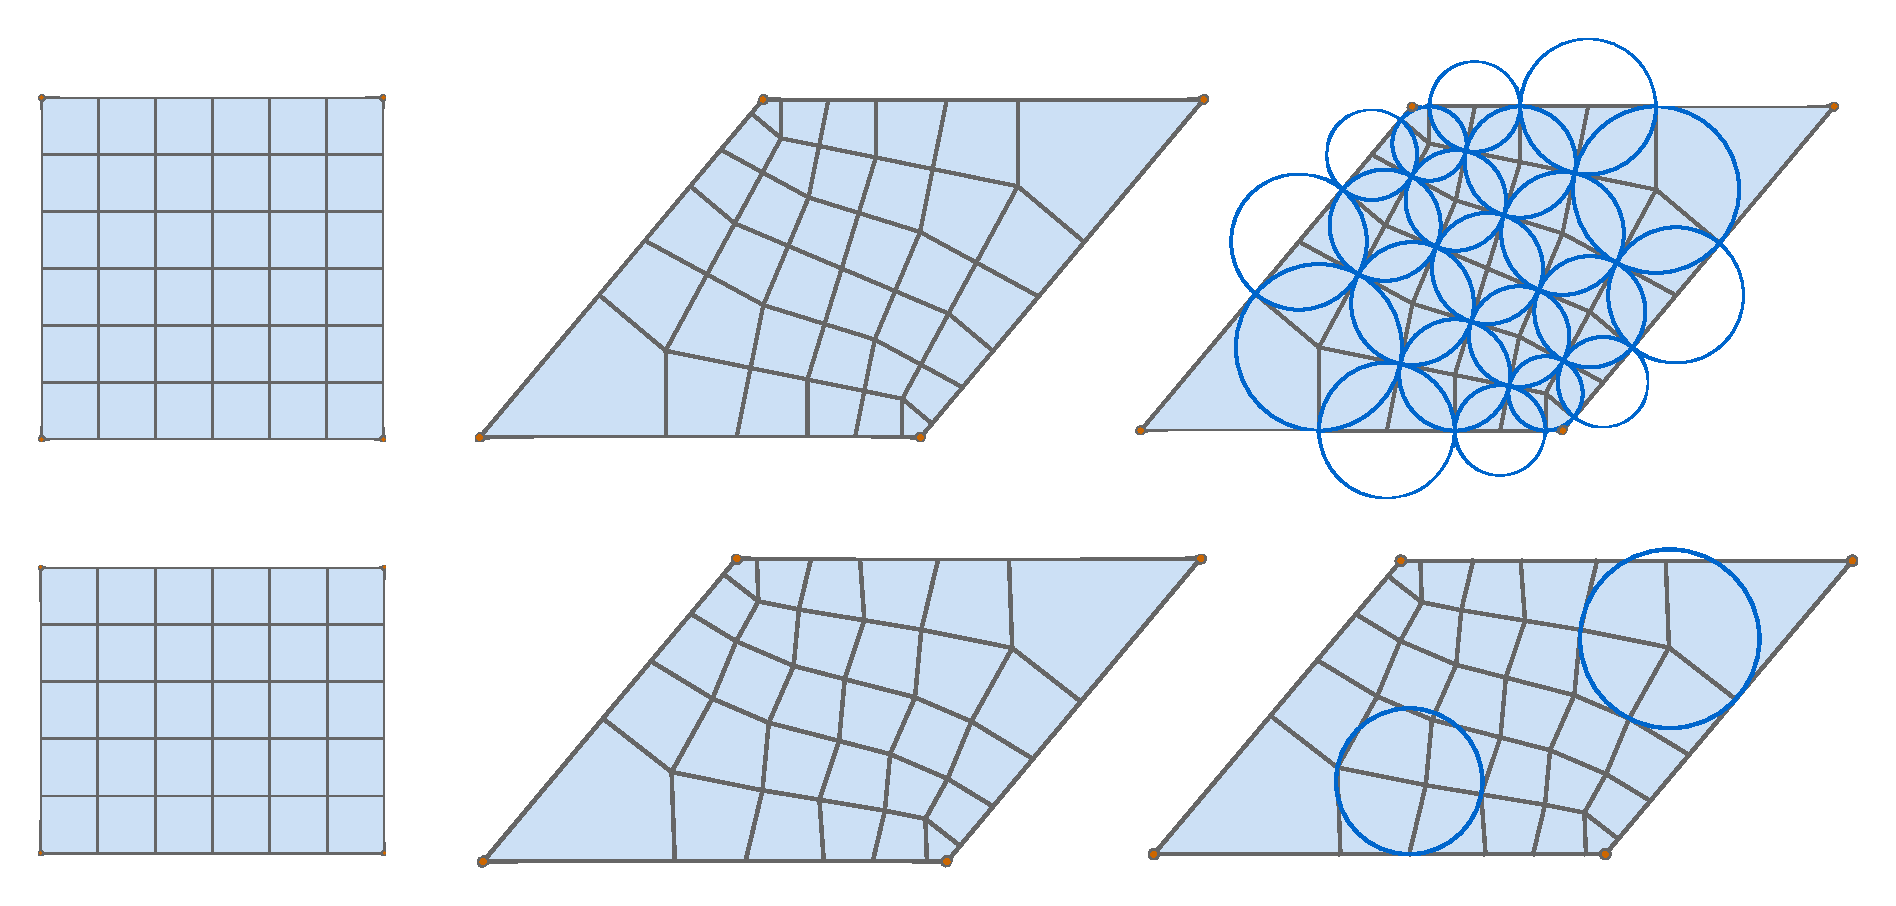
\includegraphics[width=\textwidth]{planar_circles/all.pdf}
\setstretch{0.0}{\scriptsize\tt data/planar\_circles/circular\_\{non\_\}schramm02.xml}\\
\caption{
Mapping a rectangle to a parallelogram.
All quadrilaterals in the image are cyclic quadrilaterals.
Note, in addition to the circle pattern generated by the quadrilaterals the upper example yields an S-isothermic circle pattern whereas the lower one does not.
}
\label{fig:cyclic_parallelogram}
\end{figure}

A simple example of a discrete conformal map between planar cyclic polyhedral surfaces if shown in Figure~\ref{fig:cyclic_parallelogram}. 
We start with a rectangle domain consisting of squares. 
This surface is in particular a cyclic polyhedral surface. 
We prescribe boundary angles such that we obtain a map to a parallelogram.
Corners of the domain are mapped to corners in the image. 
Technically we introduce auxiliary edge by triangulating the squares. $\lambda$s on these edges are treated as free variables. 
In a solution to the mapping problem we end up with cyclic polygons, see Equation~\ref{eq:lambda_deriv_euc}.

Note that if a Schramm-circle-pattern \cite{S97} exist for the given combinatorics and boundary data of the polyhedral surface than the minimizer realizes this pattern since its solution is the unique circle pattern with the given boundary conditions.
If it does not exist we get a cyclic solution and no circle pattern, see Figure~\ref{fig:cyclic_parallelogram} top-row versus bottom-row.

\begin{theorem}[Necessary conditions for the existence of a solution]
Let $\Sigma$ be bipartite. Let $V_w$ be the set of white boundary vertices and $V_b$ be the set of black boundary vertices.
Let $\alpha_i$ be the sum of angles at boundary vertex $i$ in the domain of the map and $\Theta_i$ be the corresponding angle sum in the conformally equivalent image.
A necessary condition for the solvability of the system is that the change of boundary curvature in both vertex sets cancel out:
\begin{eqnarray}
\sum_{i\in V_w}(\alpha_i - \Theta_i) &=& 0\label{eq:boundary_white}\\
\sum_{i\in V_b}(\alpha_i - \Theta_i) &=& 0\label{eq:boundary_black}.
\end{eqnarray}
\end{theorem}

\begin{proof}
Let $p:V\to \C$ the domain of the map consisting of squares. Each of the squares has a cross-ratio of $-1$. 
It forms a parallelogram realization of the corresponding cross-ratio system \cite[pp. 311--318]{BobenkoSuris2008}. 
Let $z:V\to \C$ be the conformally equivalent image of the discrete conformal map with given boundary conditions $\Theta_i:V\to \R_{>0}$. 
There is a function $w:V\to \C$ together with following system of equations (Hirota system):
\begin{equation*}
z_i-z_j=w_iw_j(p_i-p_j)
\end{equation*}
for each directed edge $\it ij \in \vect{E}$.
We express the sum of white and black boundary angles with the help of this system. 
Let $k_1,\ldots,k_n$ be the boundary vertices in cyclic order.
We use the indices $1,\ldots,n$ to refer to these vertices and obtain
\begin{eqnarray*}
\sum_{i=1}^{n/2}\Theta_{2i} &=&\sum_{i=1}^{n/2}\arg\left\{\frac{z_{i-1}-z_i}{z_{i+1}-z_i}\right\}\\
&=&\sum_{i=1}^{n/2}\arg\left\{\frac{w_{2i}w_{2i-1}(p_{2i-1}-p_{2i})}{w_{2i}w_{2i+1}(p_{2i+1}-p_{2i})}\right\}\\
&=&\arg\prod_{i=1}^{n/2}\frac{p_{2i-1}-p_{2i}}{p_{2i+1}-p_{2i}}\\
&=&\sum_{i=1}^{n/2}\alpha_{2i}
\end{eqnarray*}
If $k_1$ is a black vertex we get Equation~\ref{eq:boundary_white} and Equation~\ref{eq:boundary_black} for a white $k_1$.
\end{proof}

In the examples of Figure~\ref{fig:cyclic_parallelogram} this condition is met. 
In the top example all corners have the same color, thus all curvature changes add up and cancel.
In the second example the two bottom corners have a different color than the two top corners.
As the result is a parallelogram again the change of angles cancels out.
On the contrary, a square made from $7$ squares in each direction does not meet the condition with the given boundary angles.
Here opposite corners have the same color.
The change of curvature has the same sign for opposite corners, hence the conditions are not true.
Experiments show that we cannot solve the problem in such a case.

\subsection{Riemann map with cyclic quadrilaterals}
\label{sec:riemann_map}

\begin{figure}
\centering
\resizebox{\textwidth}{!}{
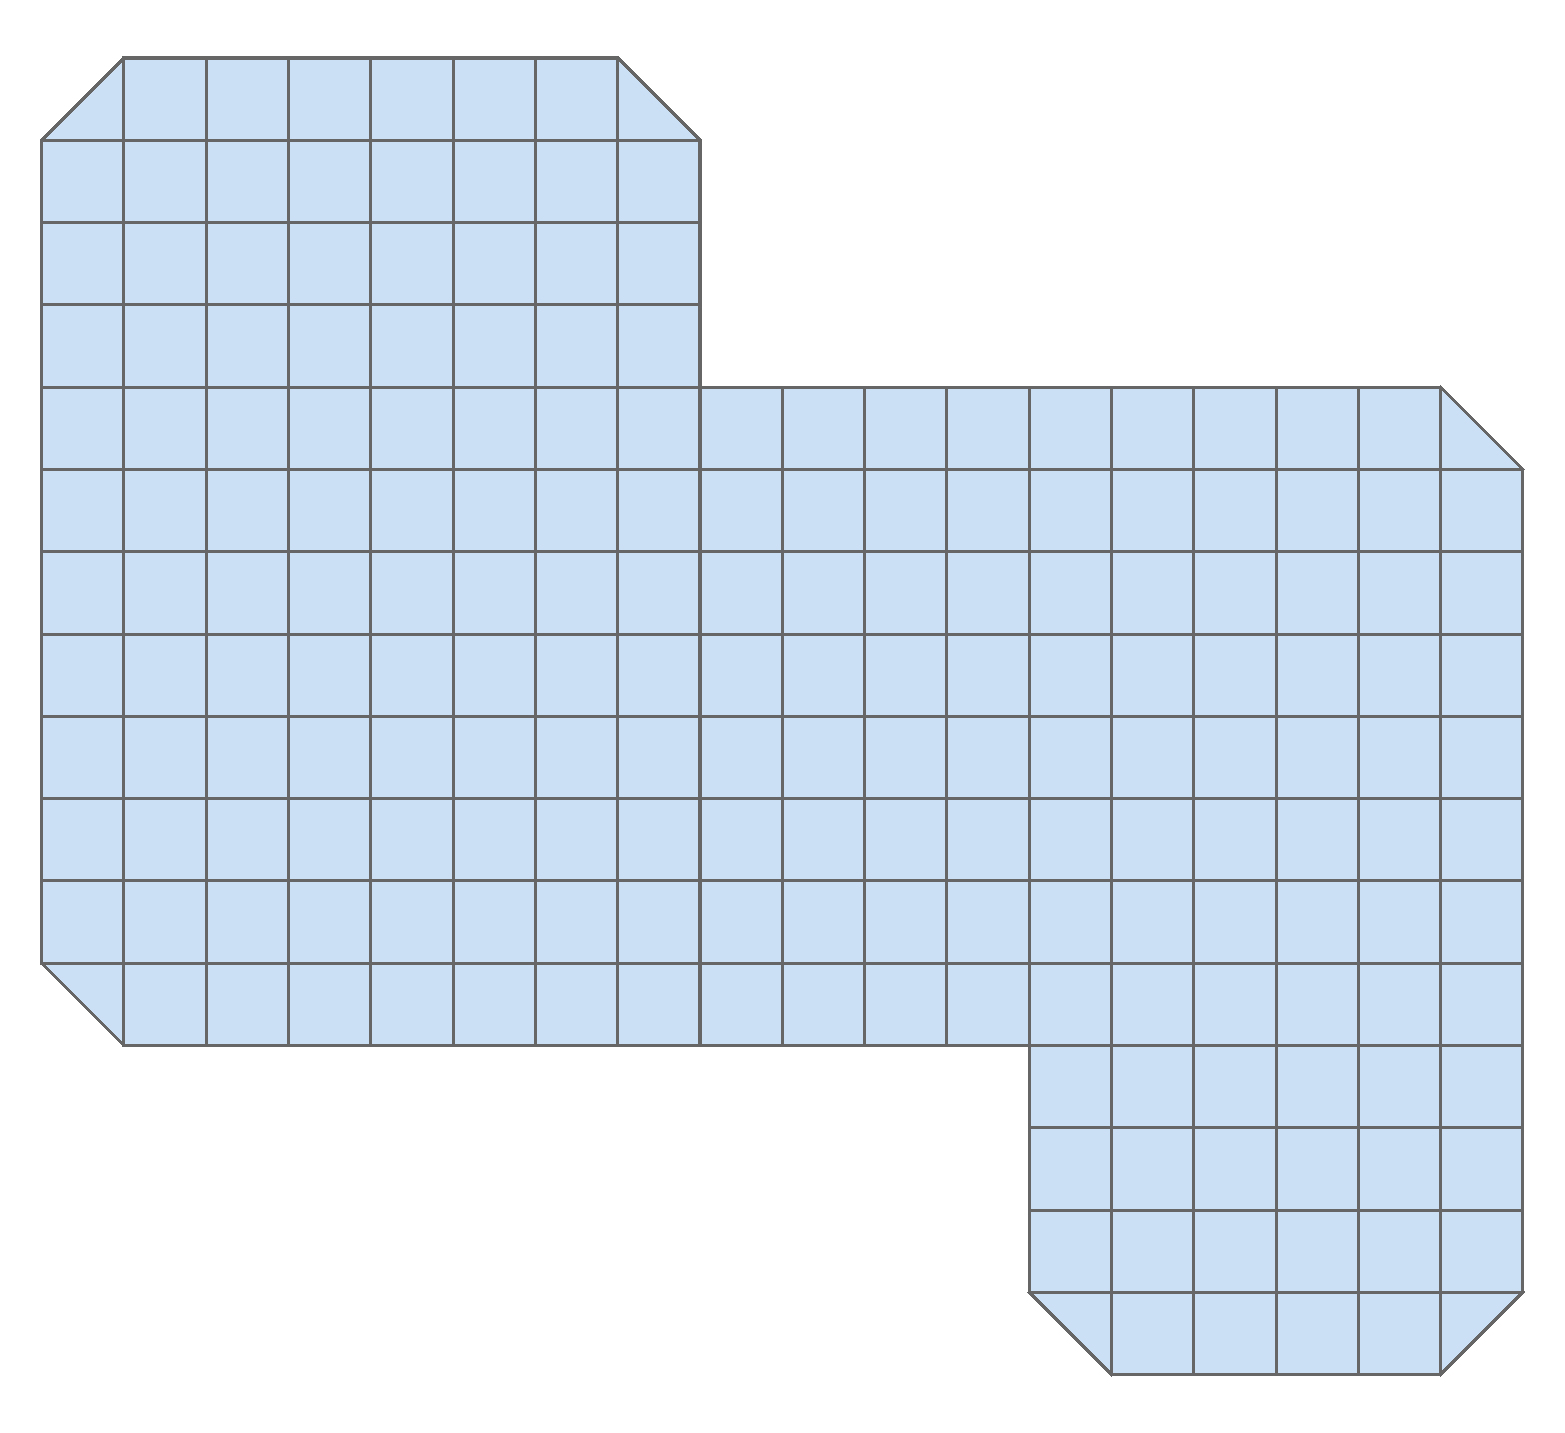
\includegraphics[height=5cm]{planar_circles/riemann_shape_image.pdf}
\quad
\raisebox{0.75cm}{
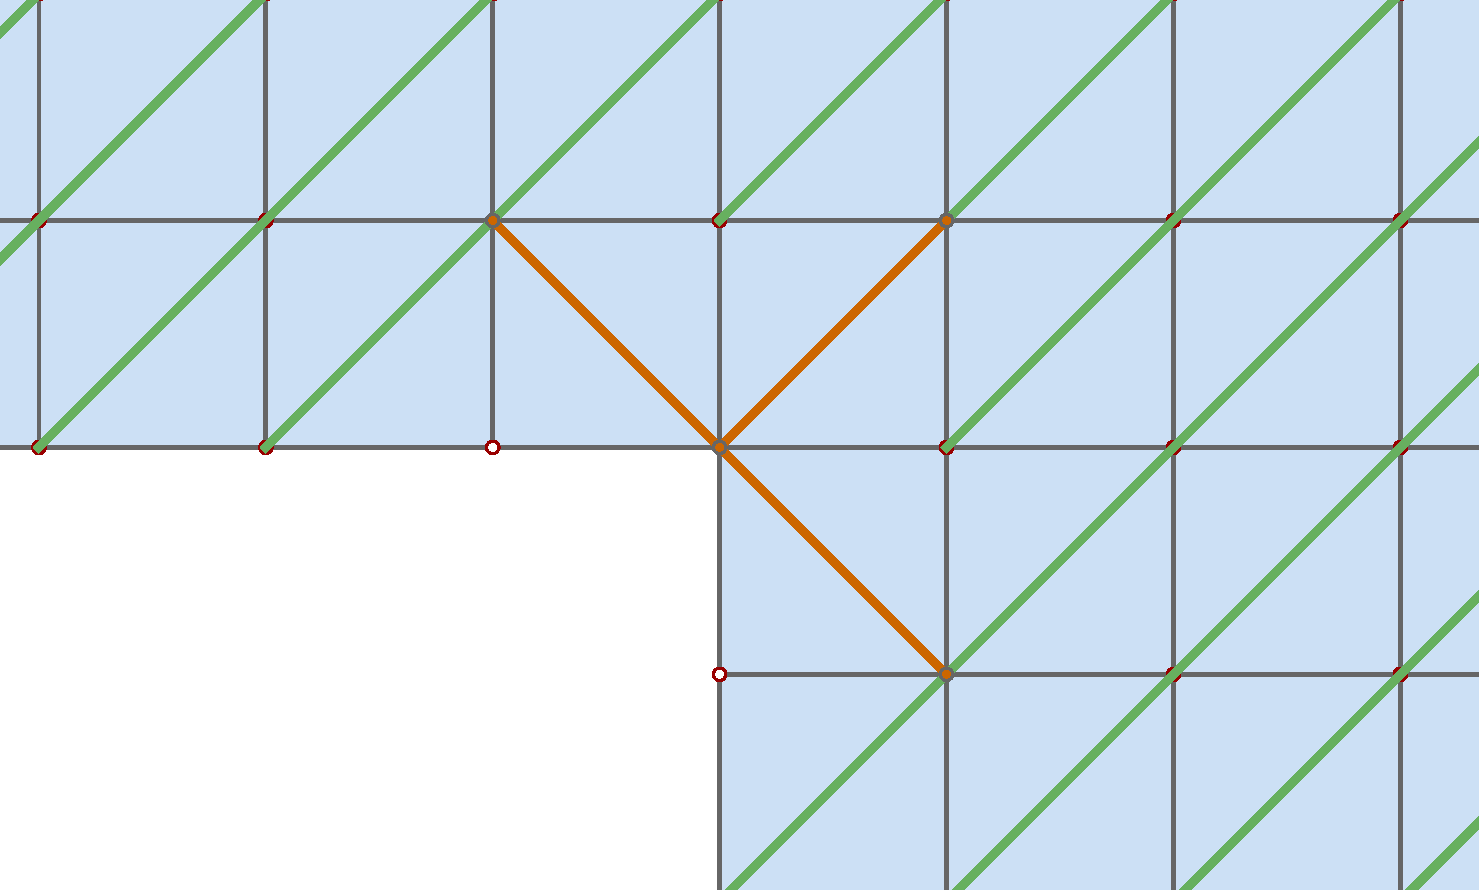
\includegraphics[height=3.5cm]{planar_circles/riemann_shape_closeup.pdf}
}
}
\resizebox{0.9\textwidth}{!}{
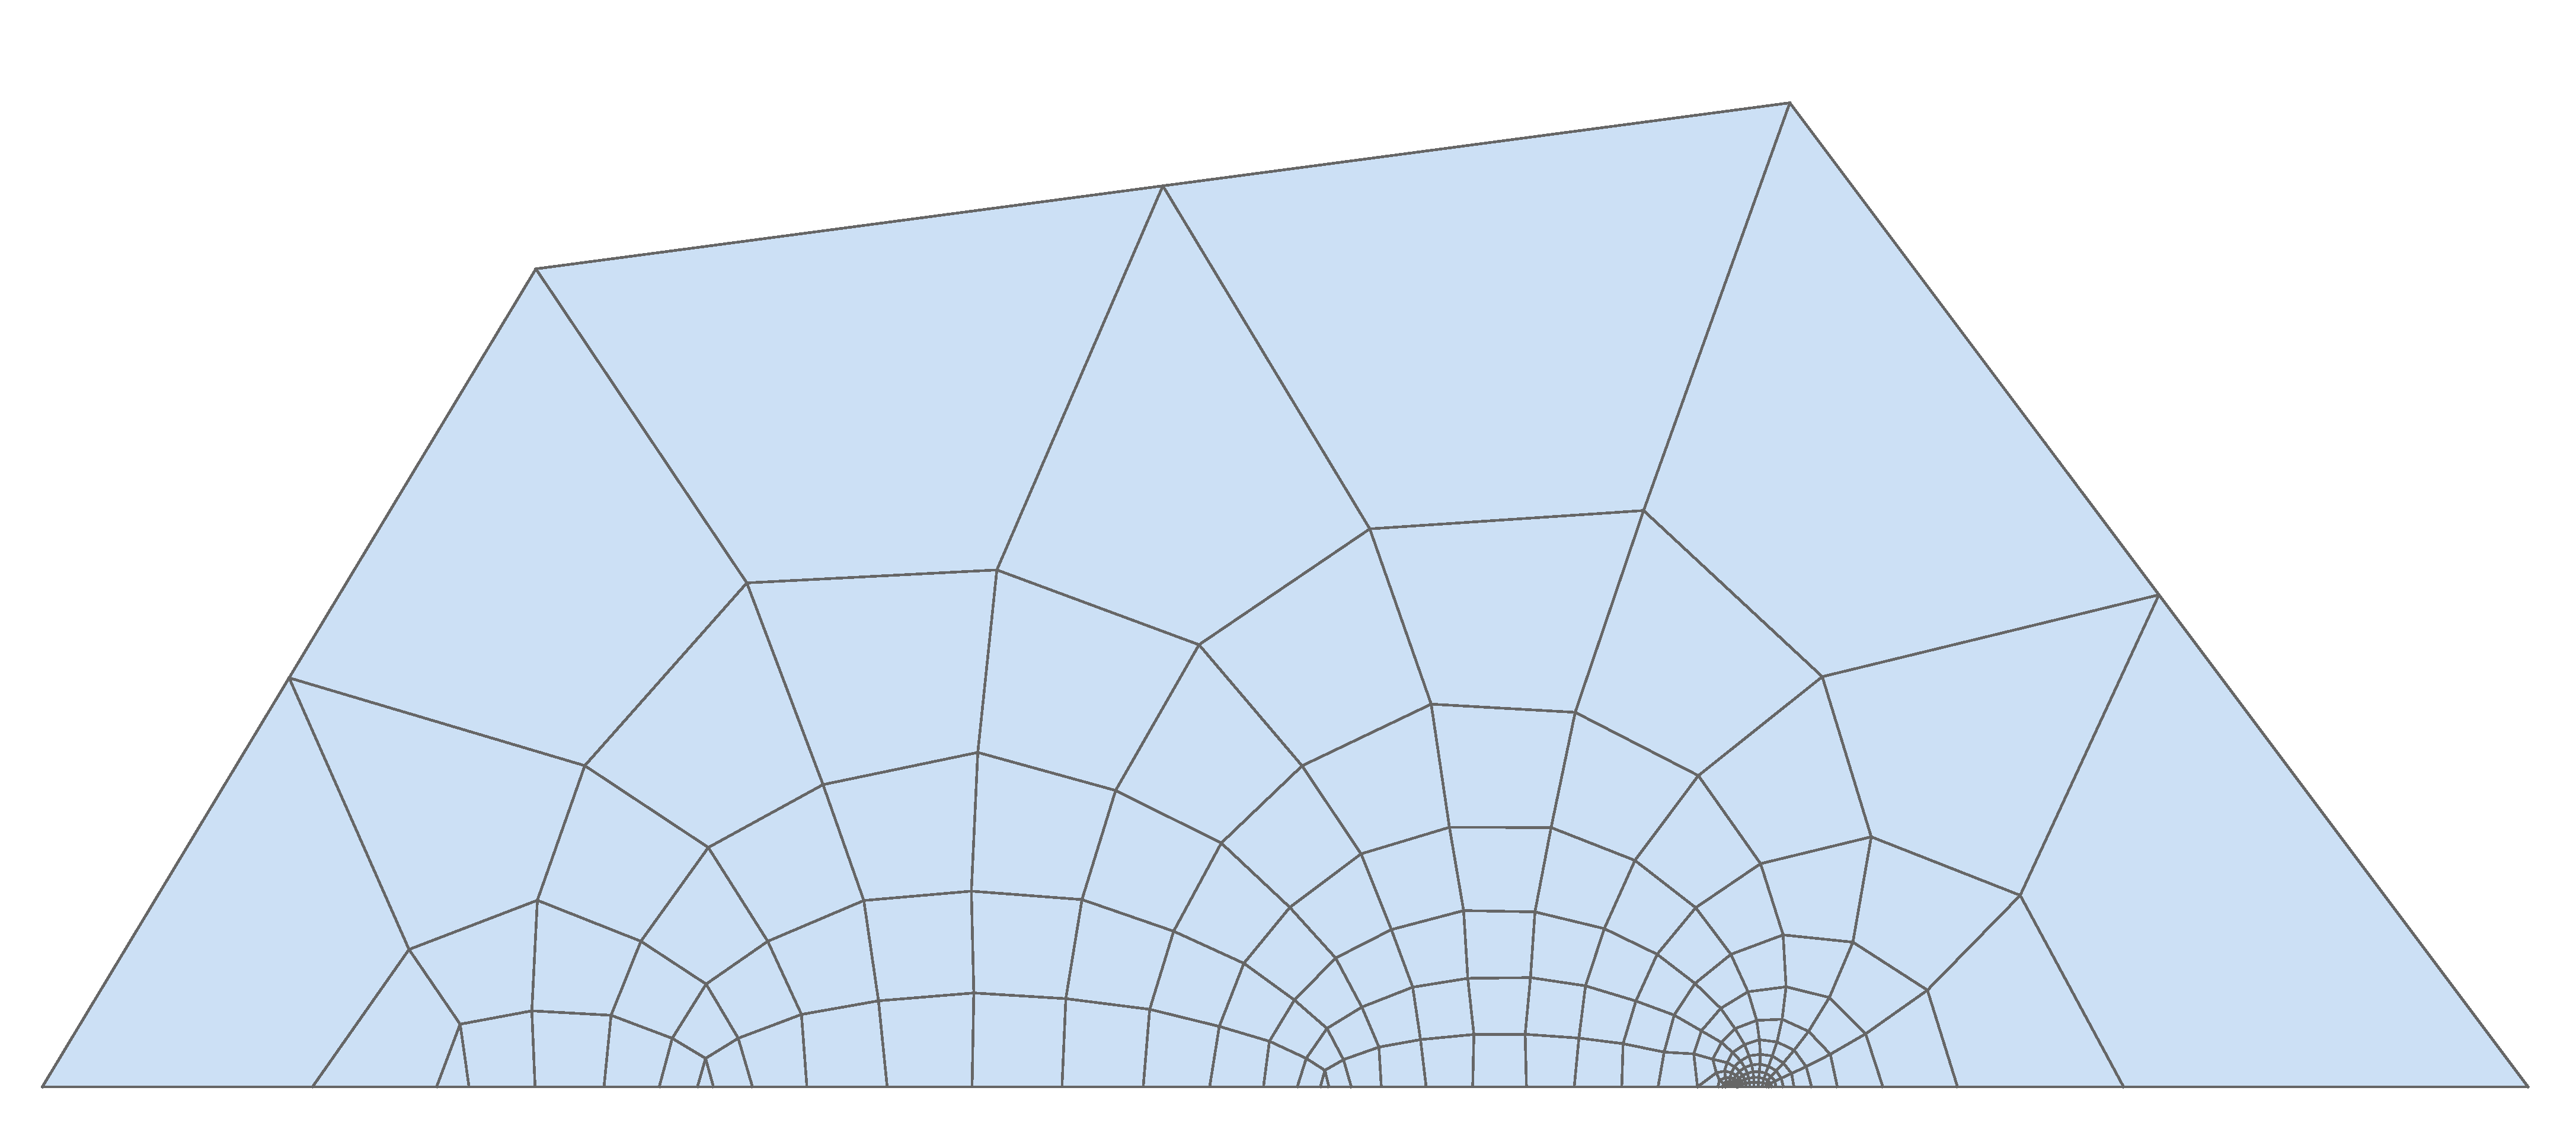
\includegraphics[height=5cm]{planar_circles/riemann_shape_halfplane.pdf}
}
\resizebox{\textwidth}{!}{
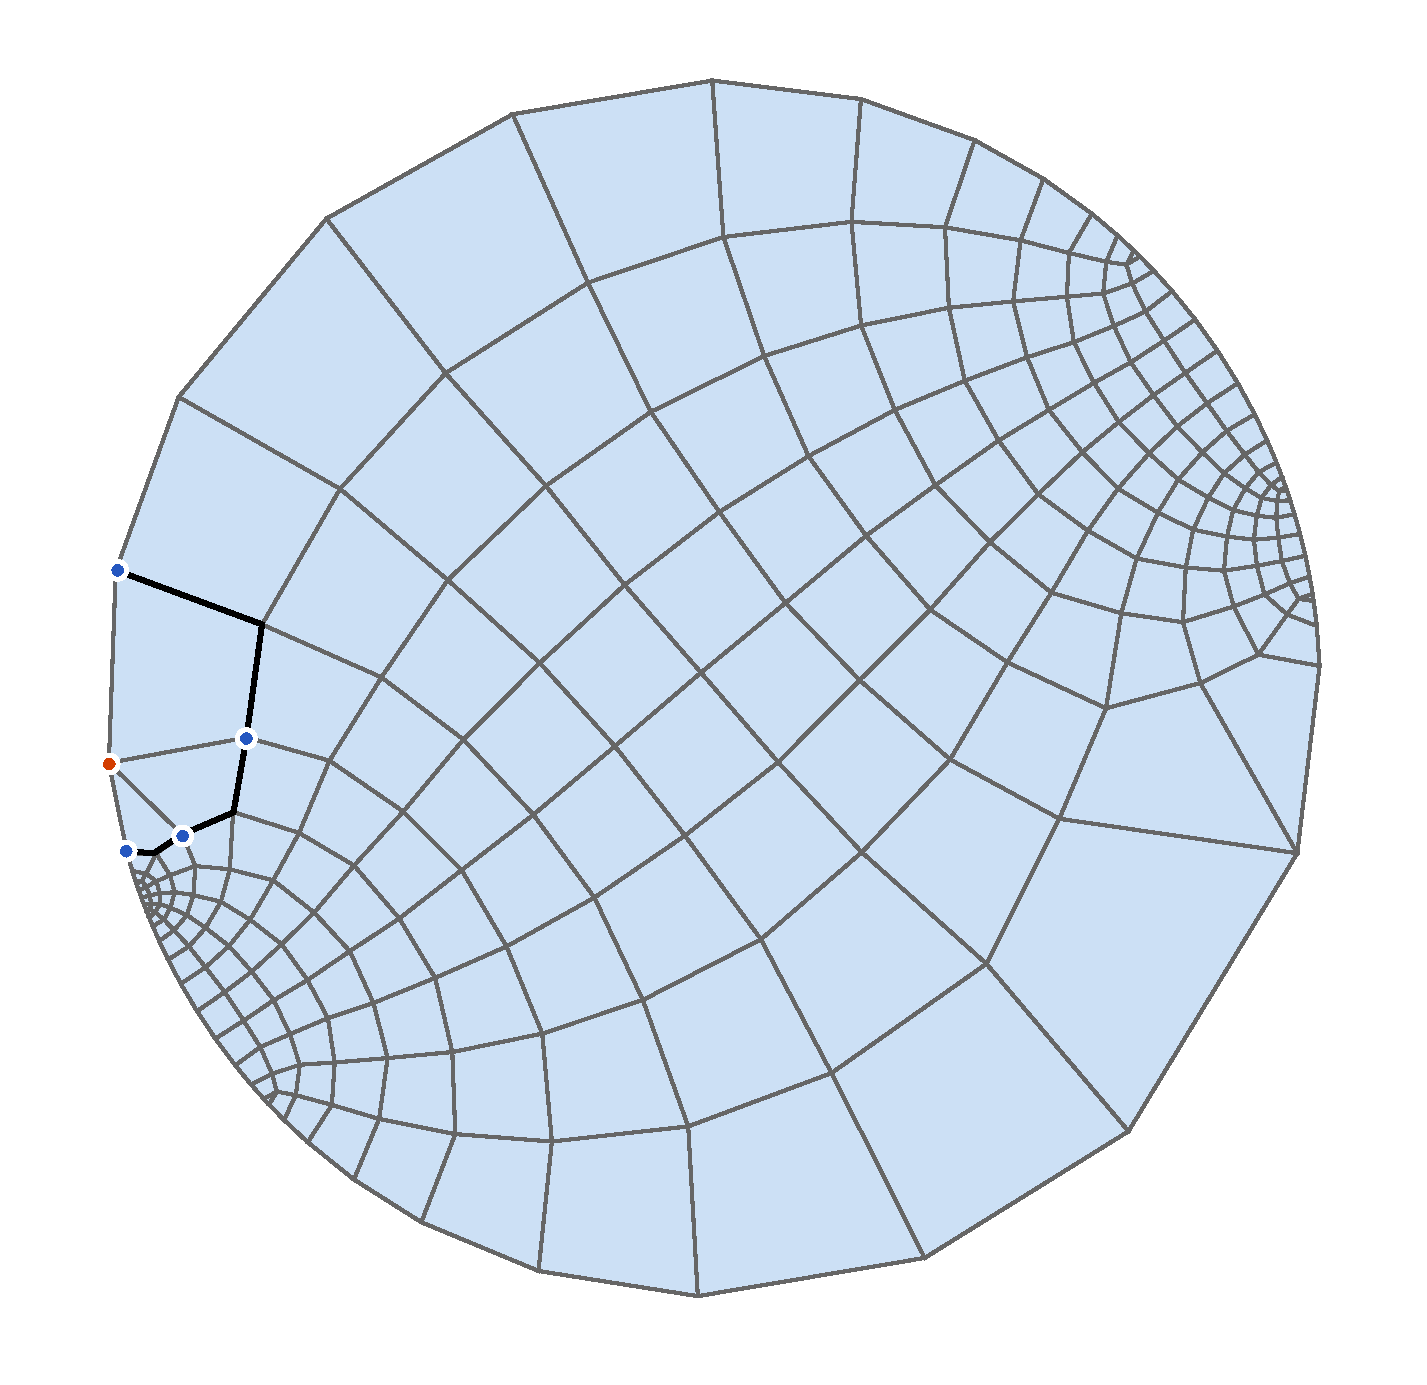
\includegraphics[height=5cm]{planar_circles/riemann_shape_domain.pdf}
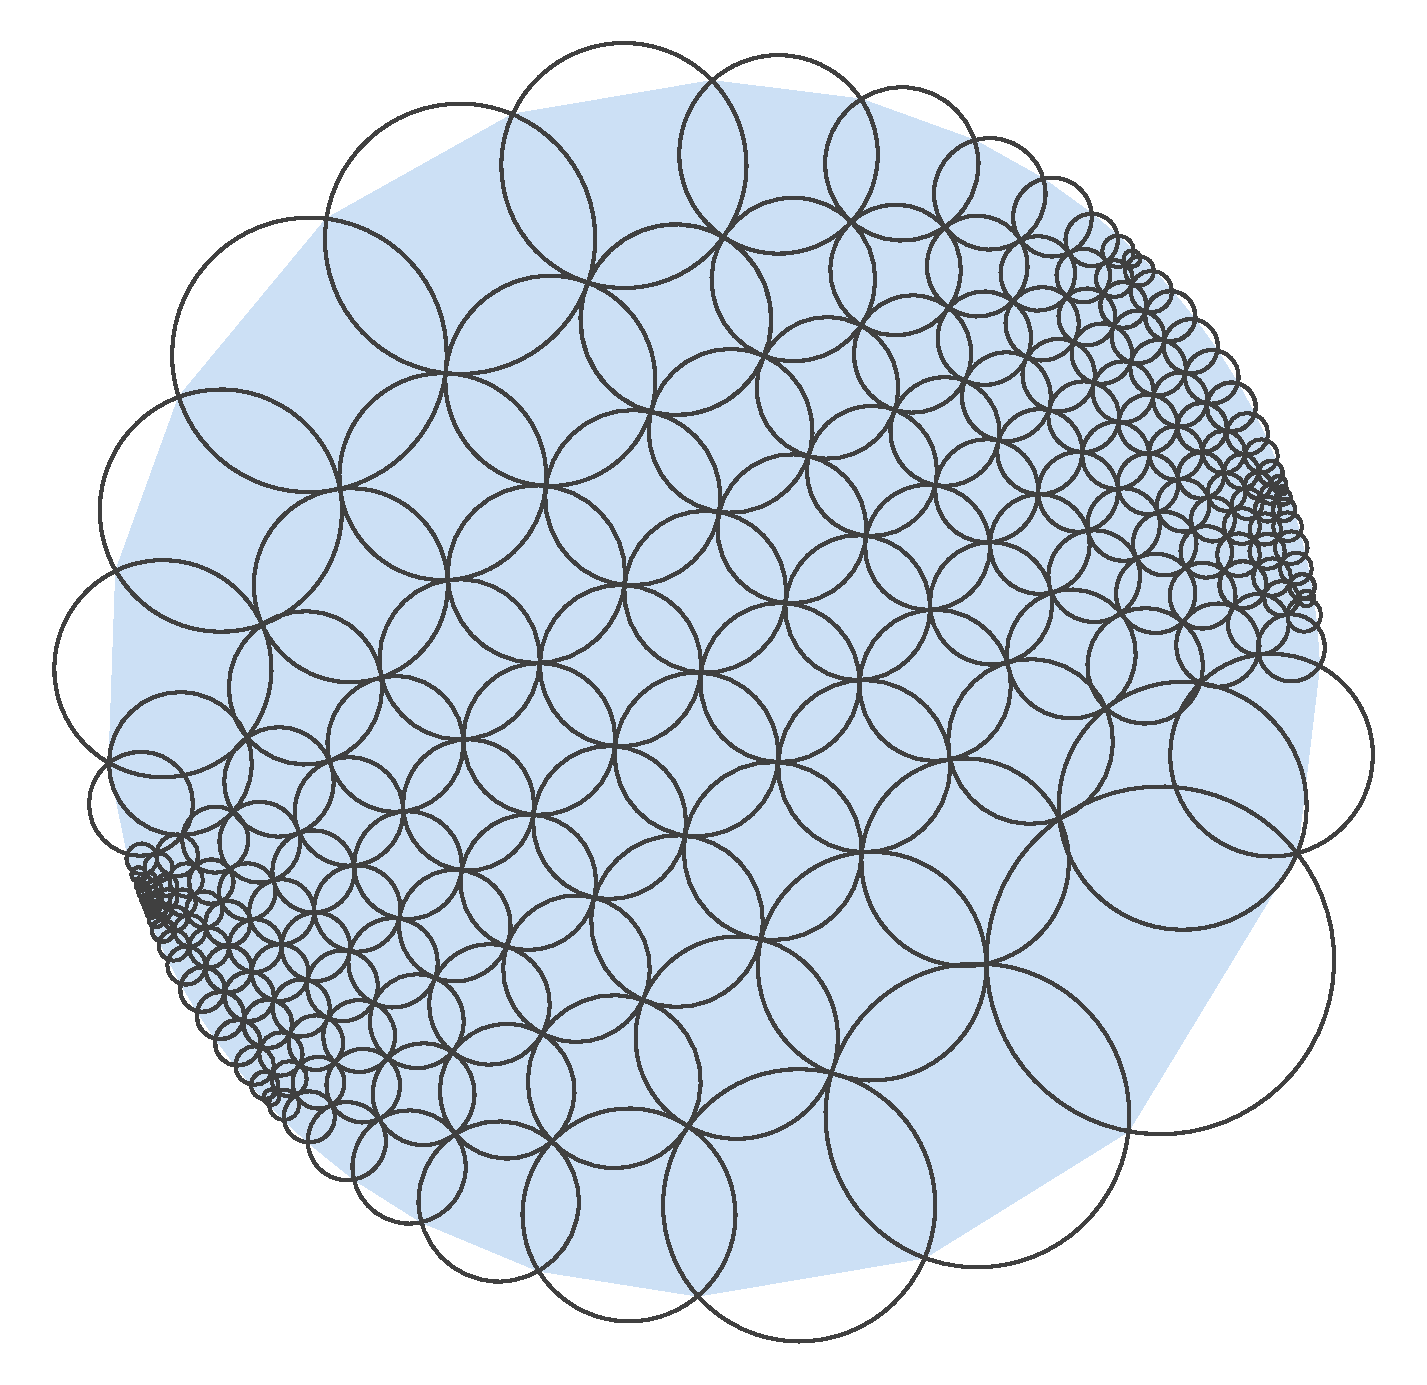
\includegraphics[height=5cm]{planar_circles/riemann_shape_circles.pdf}
}
\setstretch{0.0}{\scriptsize\tt data/planar\_circles/riemann\_shape.xml}
\caption{
Riemann-map with cyclic quadrilaterals.
Corners with valence two in the original domain are modeled as triangles, upper left.
We first map to the upper half-plane.
Quadrilaterals adjacent to the point at infinity are removed.
Points opposite to the point at infinity have a prescribed boundary angle of $\pi$.
The four vertices in between have a fixed $u=0$.
By that quadrilaterals adjacent to the point at infinity are cyclic after the Moebius transformation to the disk, bottom.
}
\label{fig:circular_riemann}
\end{figure}

We show how to calculate discrete Riemann maps for cyclic quadrilateral domains, i.e., a discrete analog of conformal maps from a simply connected planar region to the unit disk. 
In particular this yields a method for the generation of circle pattern Riemann maps, see Figure~\ref{fig:circular_riemann}.
The procedure is in many aspects analogous to the previously described method for triangulations \cite{Bobenko2010}.
Let $\Sigma$ be a cyclic planar domain that consists solely of quadrilaterals and $\ell$ be a discrete metric on $\Sigma$. 
Proceed as follows:
\begin{enumerate}
\item 
Choose a vertex $k$ on the boundary of $\Sigma$ and apply a discrete conformal change of metric such that all edges incident with $k$ have the same lengths.
\item
Let $\Sigma'$ be the complex with all quadrilaterals that are incident to vertex $k$ removed.
\item
Solve Problem~\ref{prob:factors_and_angles} for $\Sigma'$ with prescribed $\Theta_i=2\pi$ for interior vertices in $\Sigma'$, $\Theta_i=\pi$ for boundary vertices in $\Sigma'$ that are not neighbors of $k$ in $\Sigma$ and $u_i=0$ for neighbors of $k$. 
The result is a planar cyclic domain. 
The boundary edges that belong to faces at vertex $k$ in $\Sigma$ are contained in straight lines for each face.
All other boundary edges are contained in a common straight line. 
\item
Apply a M{\"o}bius transformation to the vertices that maps this straight line to a circle and the other vertices to the inside of this circle.
Reinsert $k$ at the image point of $\infty$ under this M{\"o}bius transformation.
Each face $\it ijmk \in \Sigma$ incident with $k$ is cyclic because the three vertices $i$, $j$, and $m$ are contained in a line before transformation.
\item
Optionally apply a planar version of the M{\"o}bius normalization as described in Section~\ref{sec:moebius_normalization}. 
\end{enumerate} 

The result is a planar cyclic domain that is conformally equivalent to $(\Sigma, \ell)$ and its boundary polygon is inscribed in a circle.
Note that as for triangulations we cannot have ears, i.e., a quadrilateral with two consecutive boundary edges, in the complex $\Sigma$ when solving Problem~\ref{prob:factors_and_angles}. To address this we replace ears by triangles, see Figure~\ref{fig:circular_riemann}.

\begin{proposition}
The result of this procedure is discretely conformally equivalent to $(\Sigma, \ell)$ and its boundary polygon inscribed in a circle.
\end{proposition}
\begin{proof}
We have to show that the cross-ratio of all quadrilaterals agree. 
Since the quadrilaterals are cyclic their cross-ratios are real and negative.
After step 1 the cross ratio of the quadrilaterals at vertex $k$ are given by the length ratio of the two edges that are not connected to $k$.
After step 3 each three vertices $i$, $j$, and $k$ belonging to a face at $k$ lie on a straight line. 
Thus the cross-ratio of the points $\infty$, $i$, $j$, and $k$ is the ratio of the two lengths $\it ij$ and $\it jk$.
This ratio is equal to the ratio after step 1 because there is only one scale factor involved. 
The others are fixed to zero.
The cross-ratio is invariant under M{\"o}bius transformation therefor the ratios agree.
\todo{link to cross-ratio generalization}
\end{proof}

\subsection{Discrete circle domains}
\label{sec:circle_domains}

\begin{figure}
\centering
\resizebox{\textwidth}{!}{
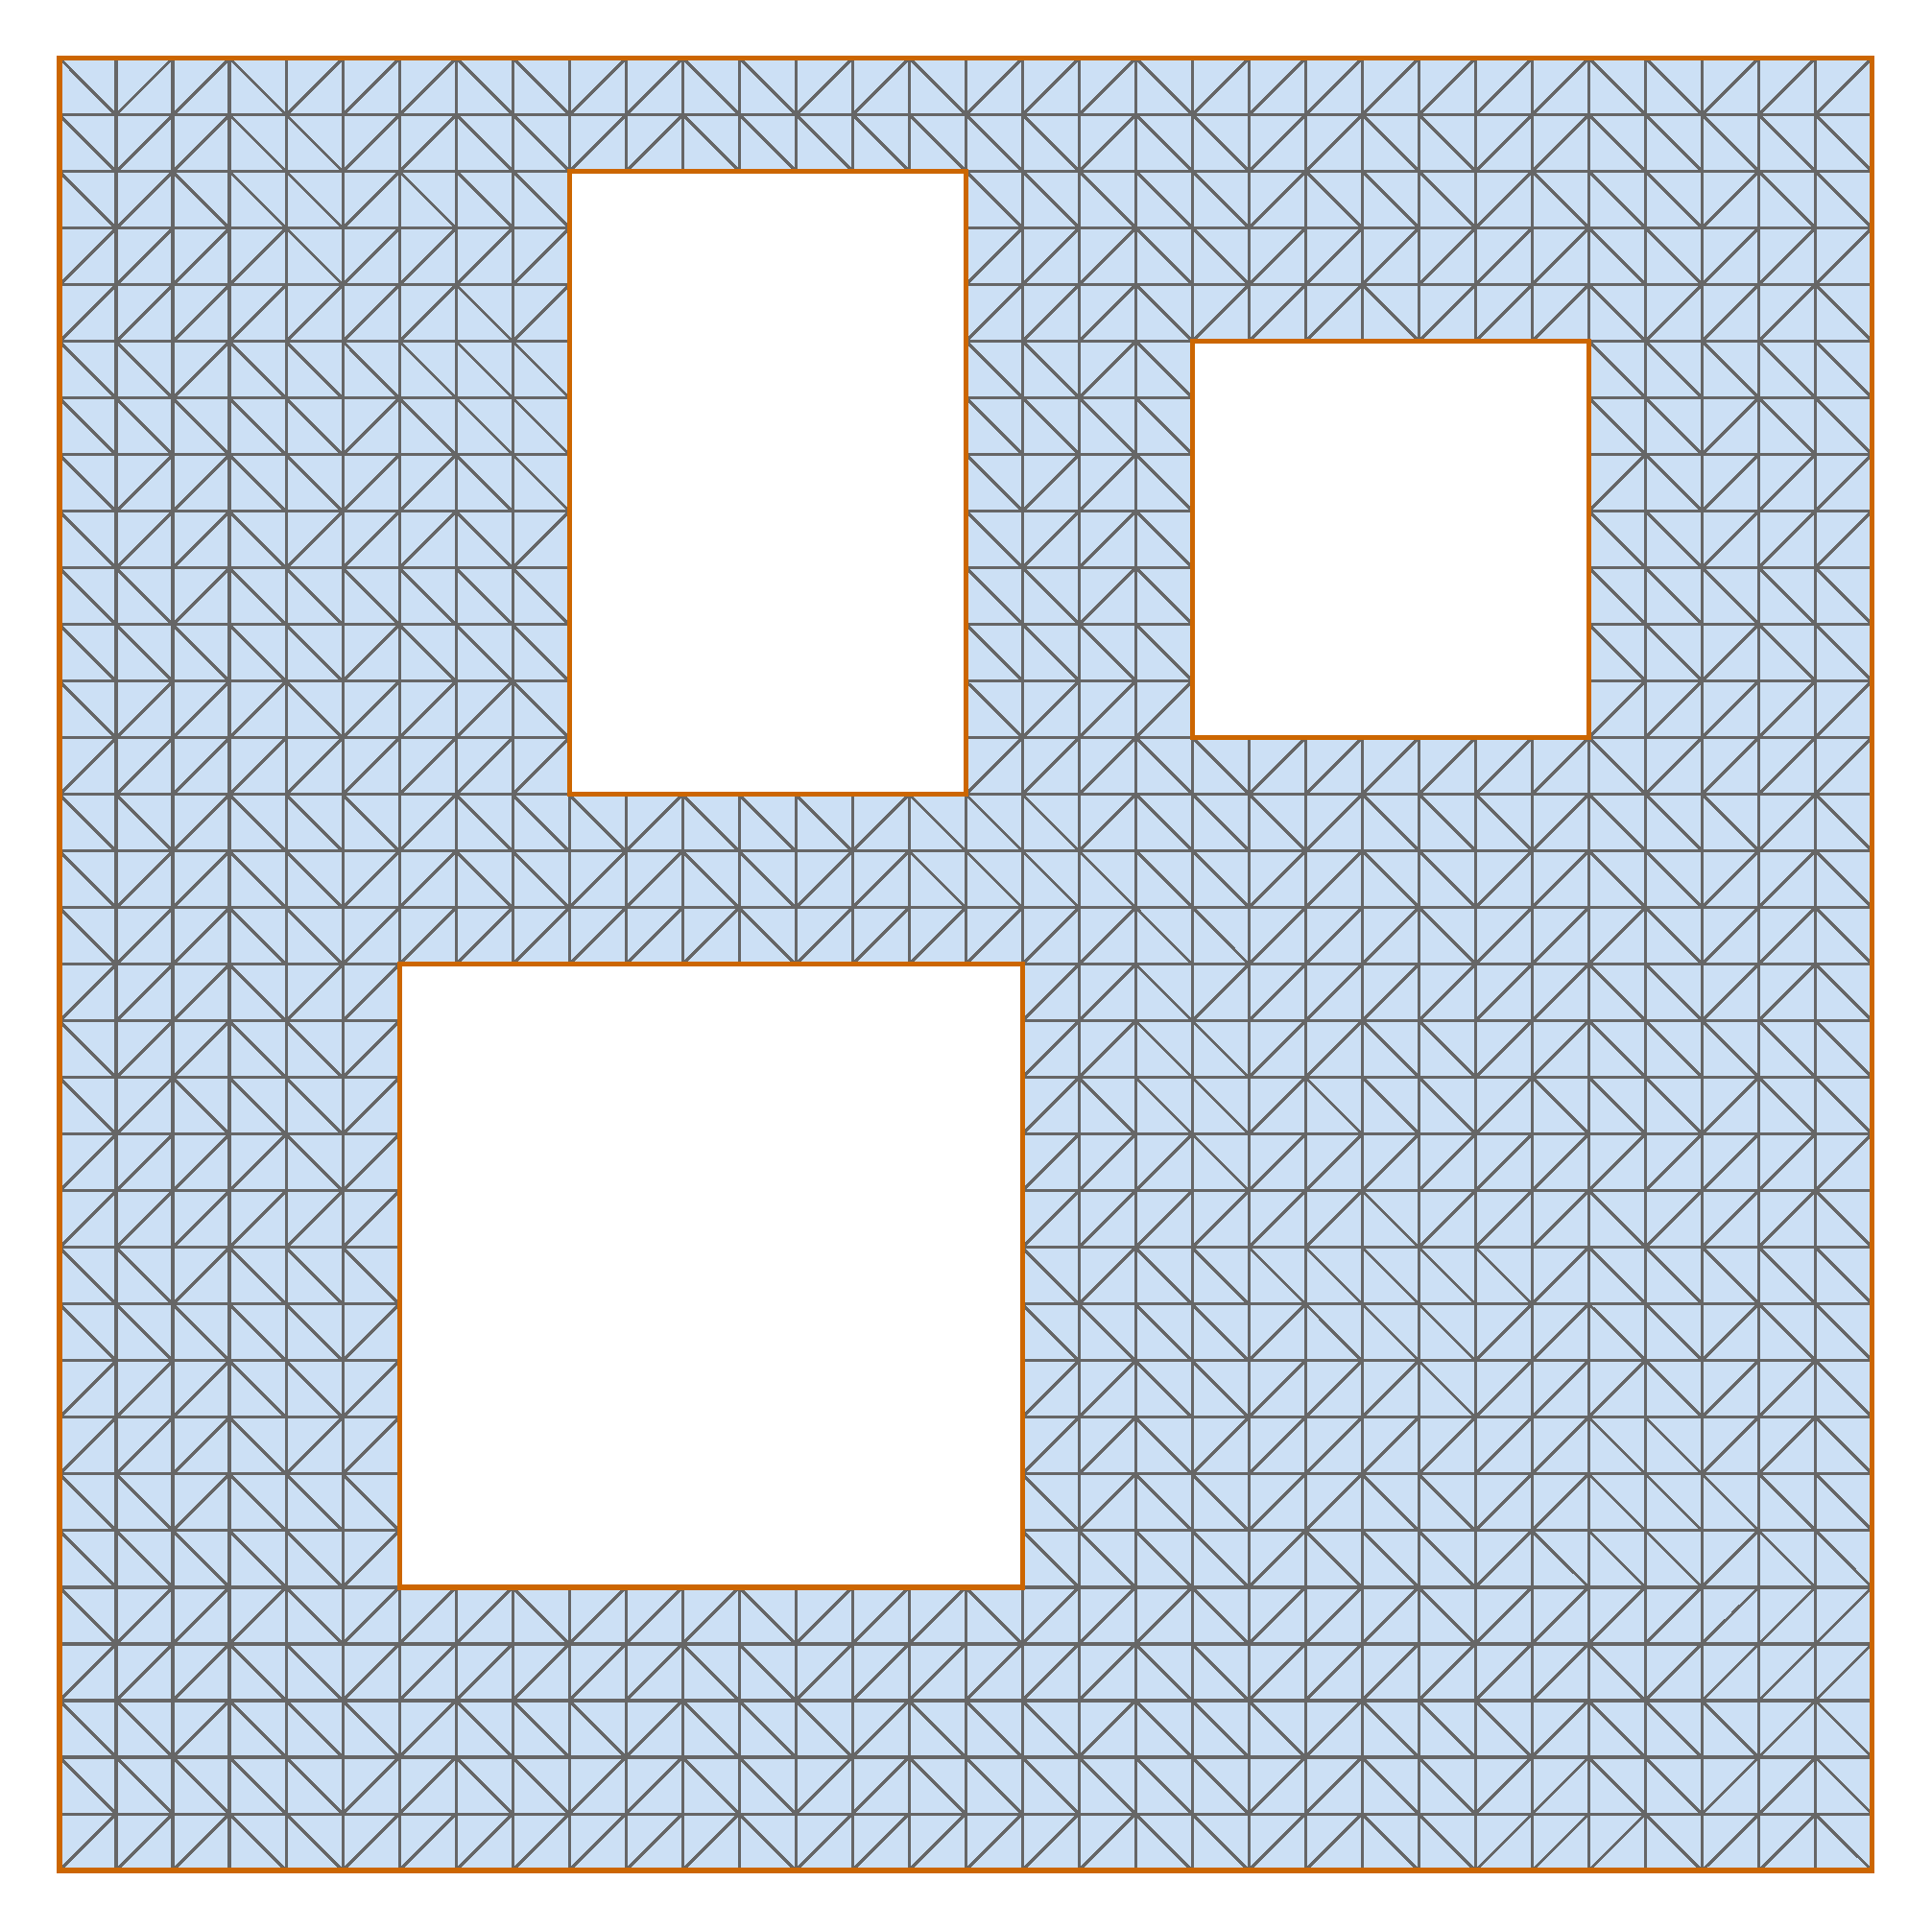
\includegraphics[width=0.5\textwidth]{circle_domain_euclidean/three_holes_image.pdf}
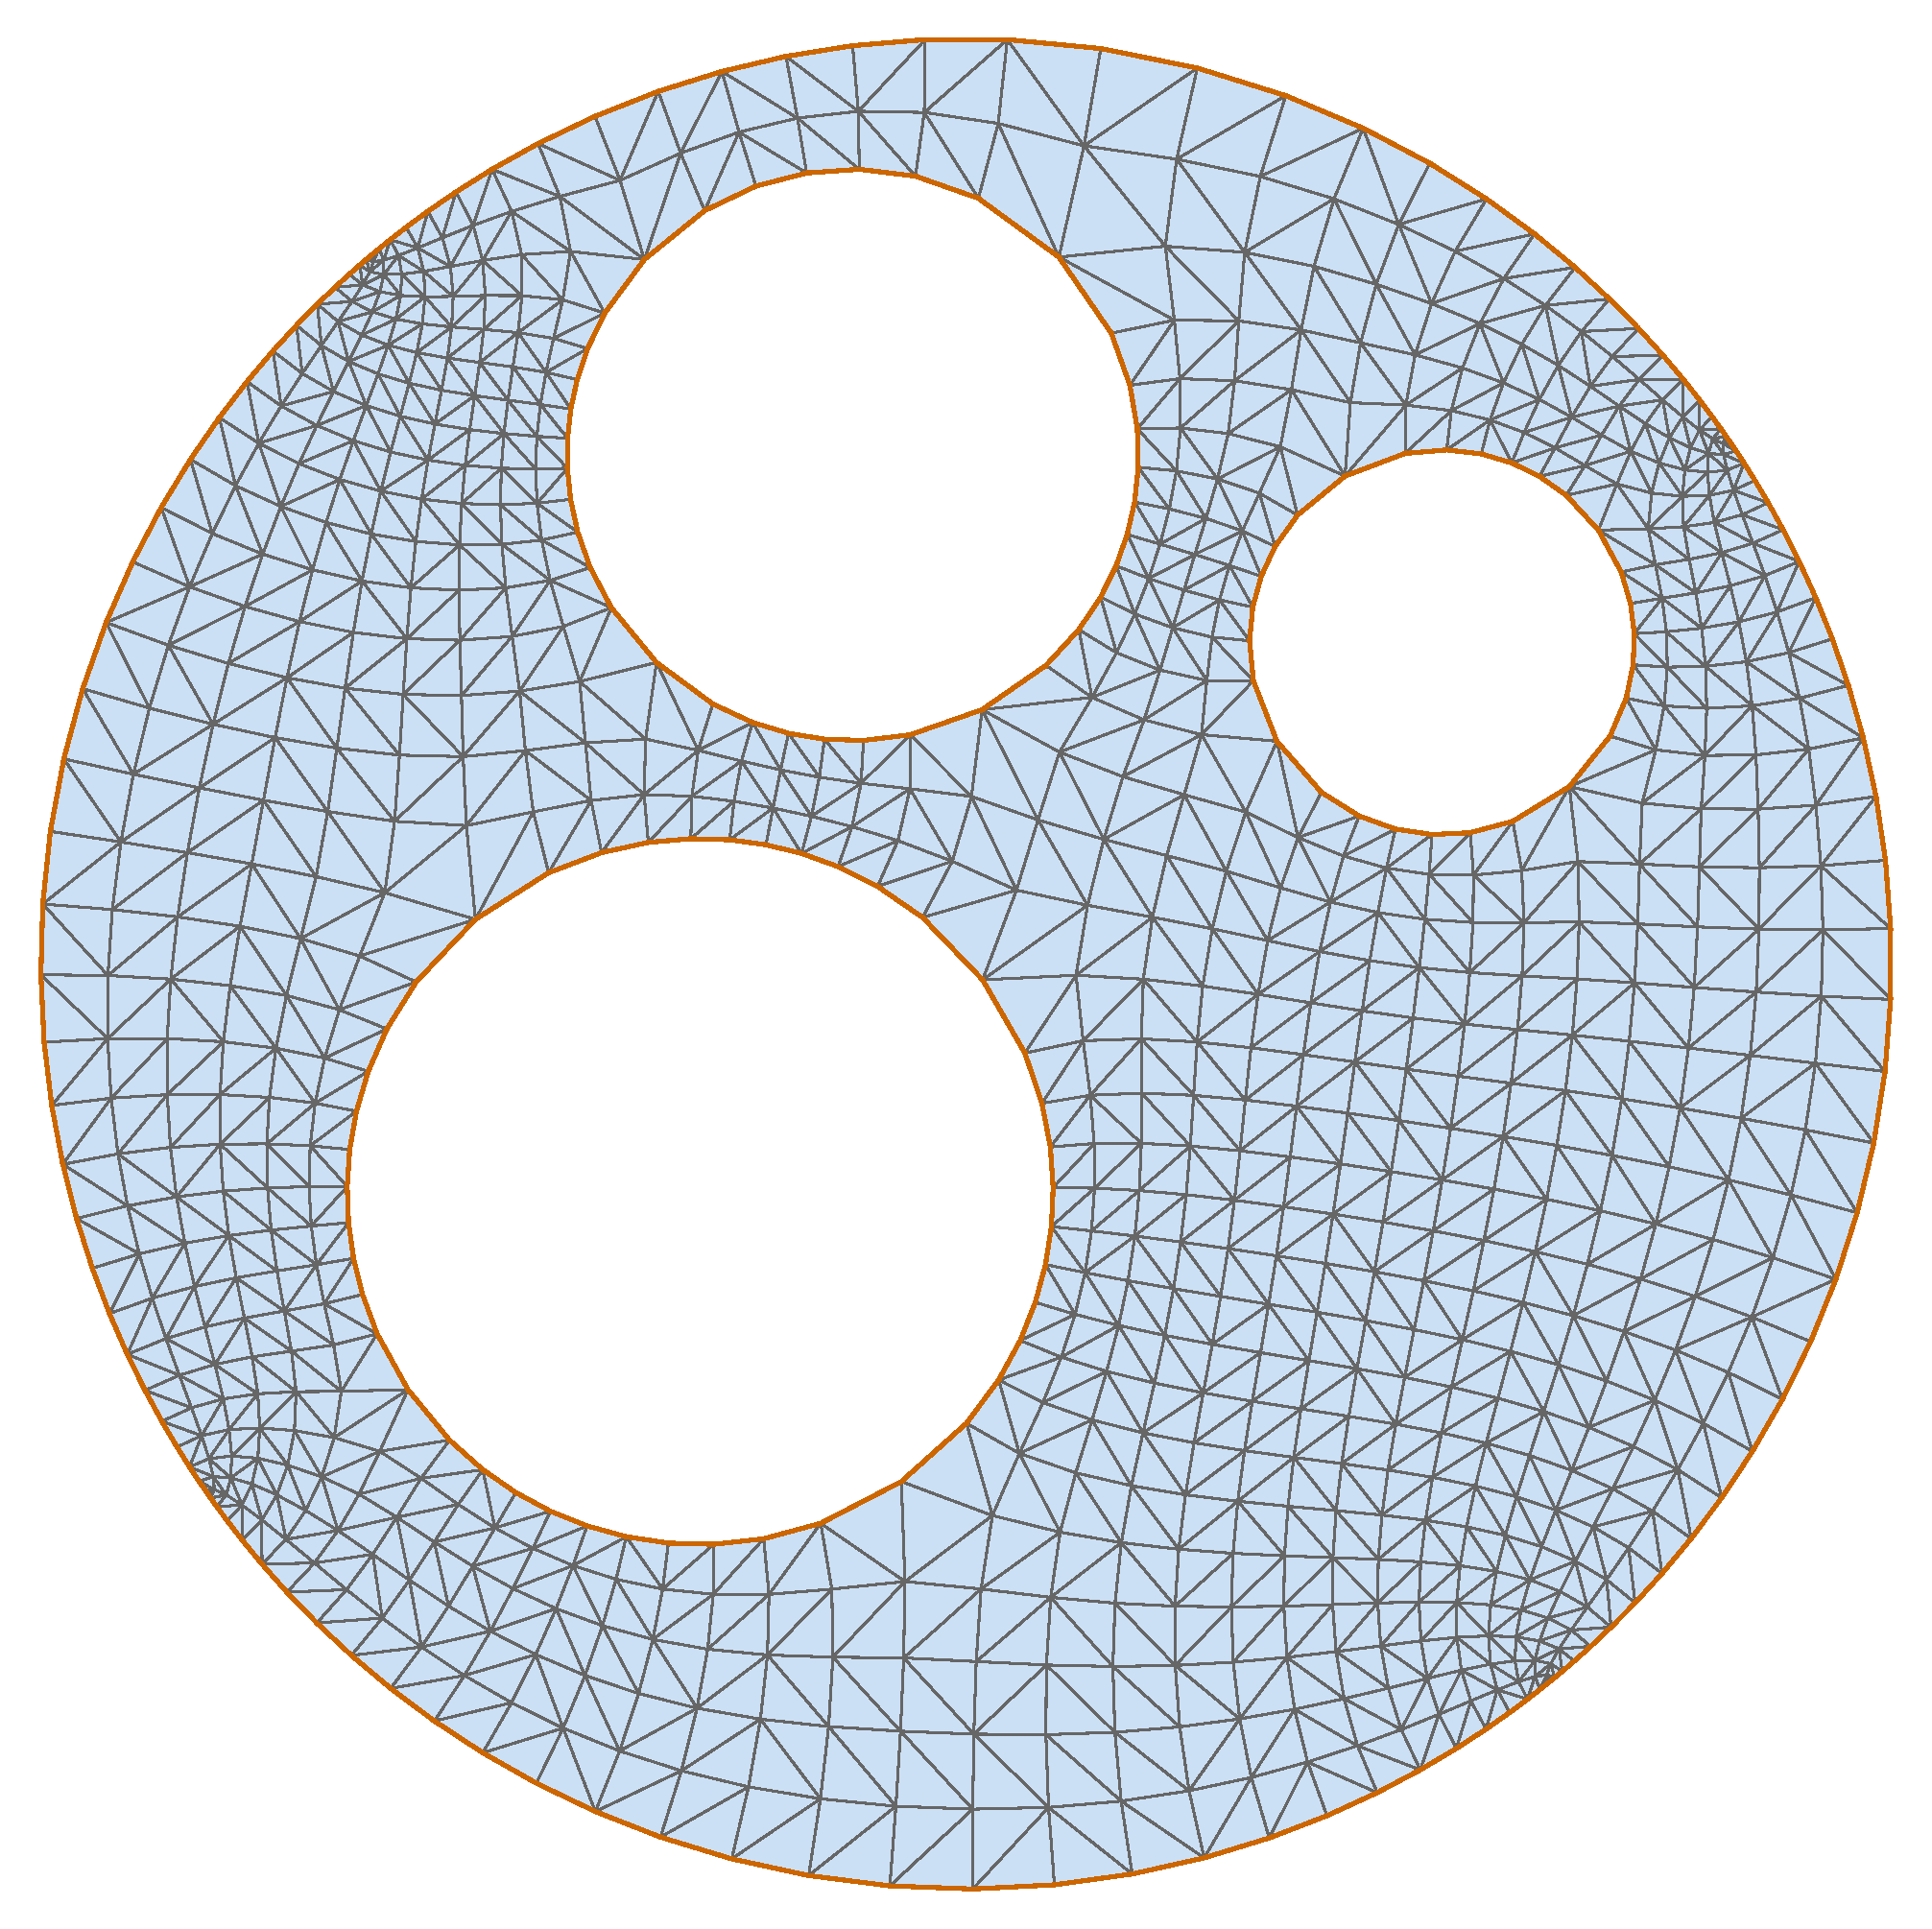
\includegraphics[width=0.5\textwidth]{circle_domain_euclidean/three_holes_domain.pdf}
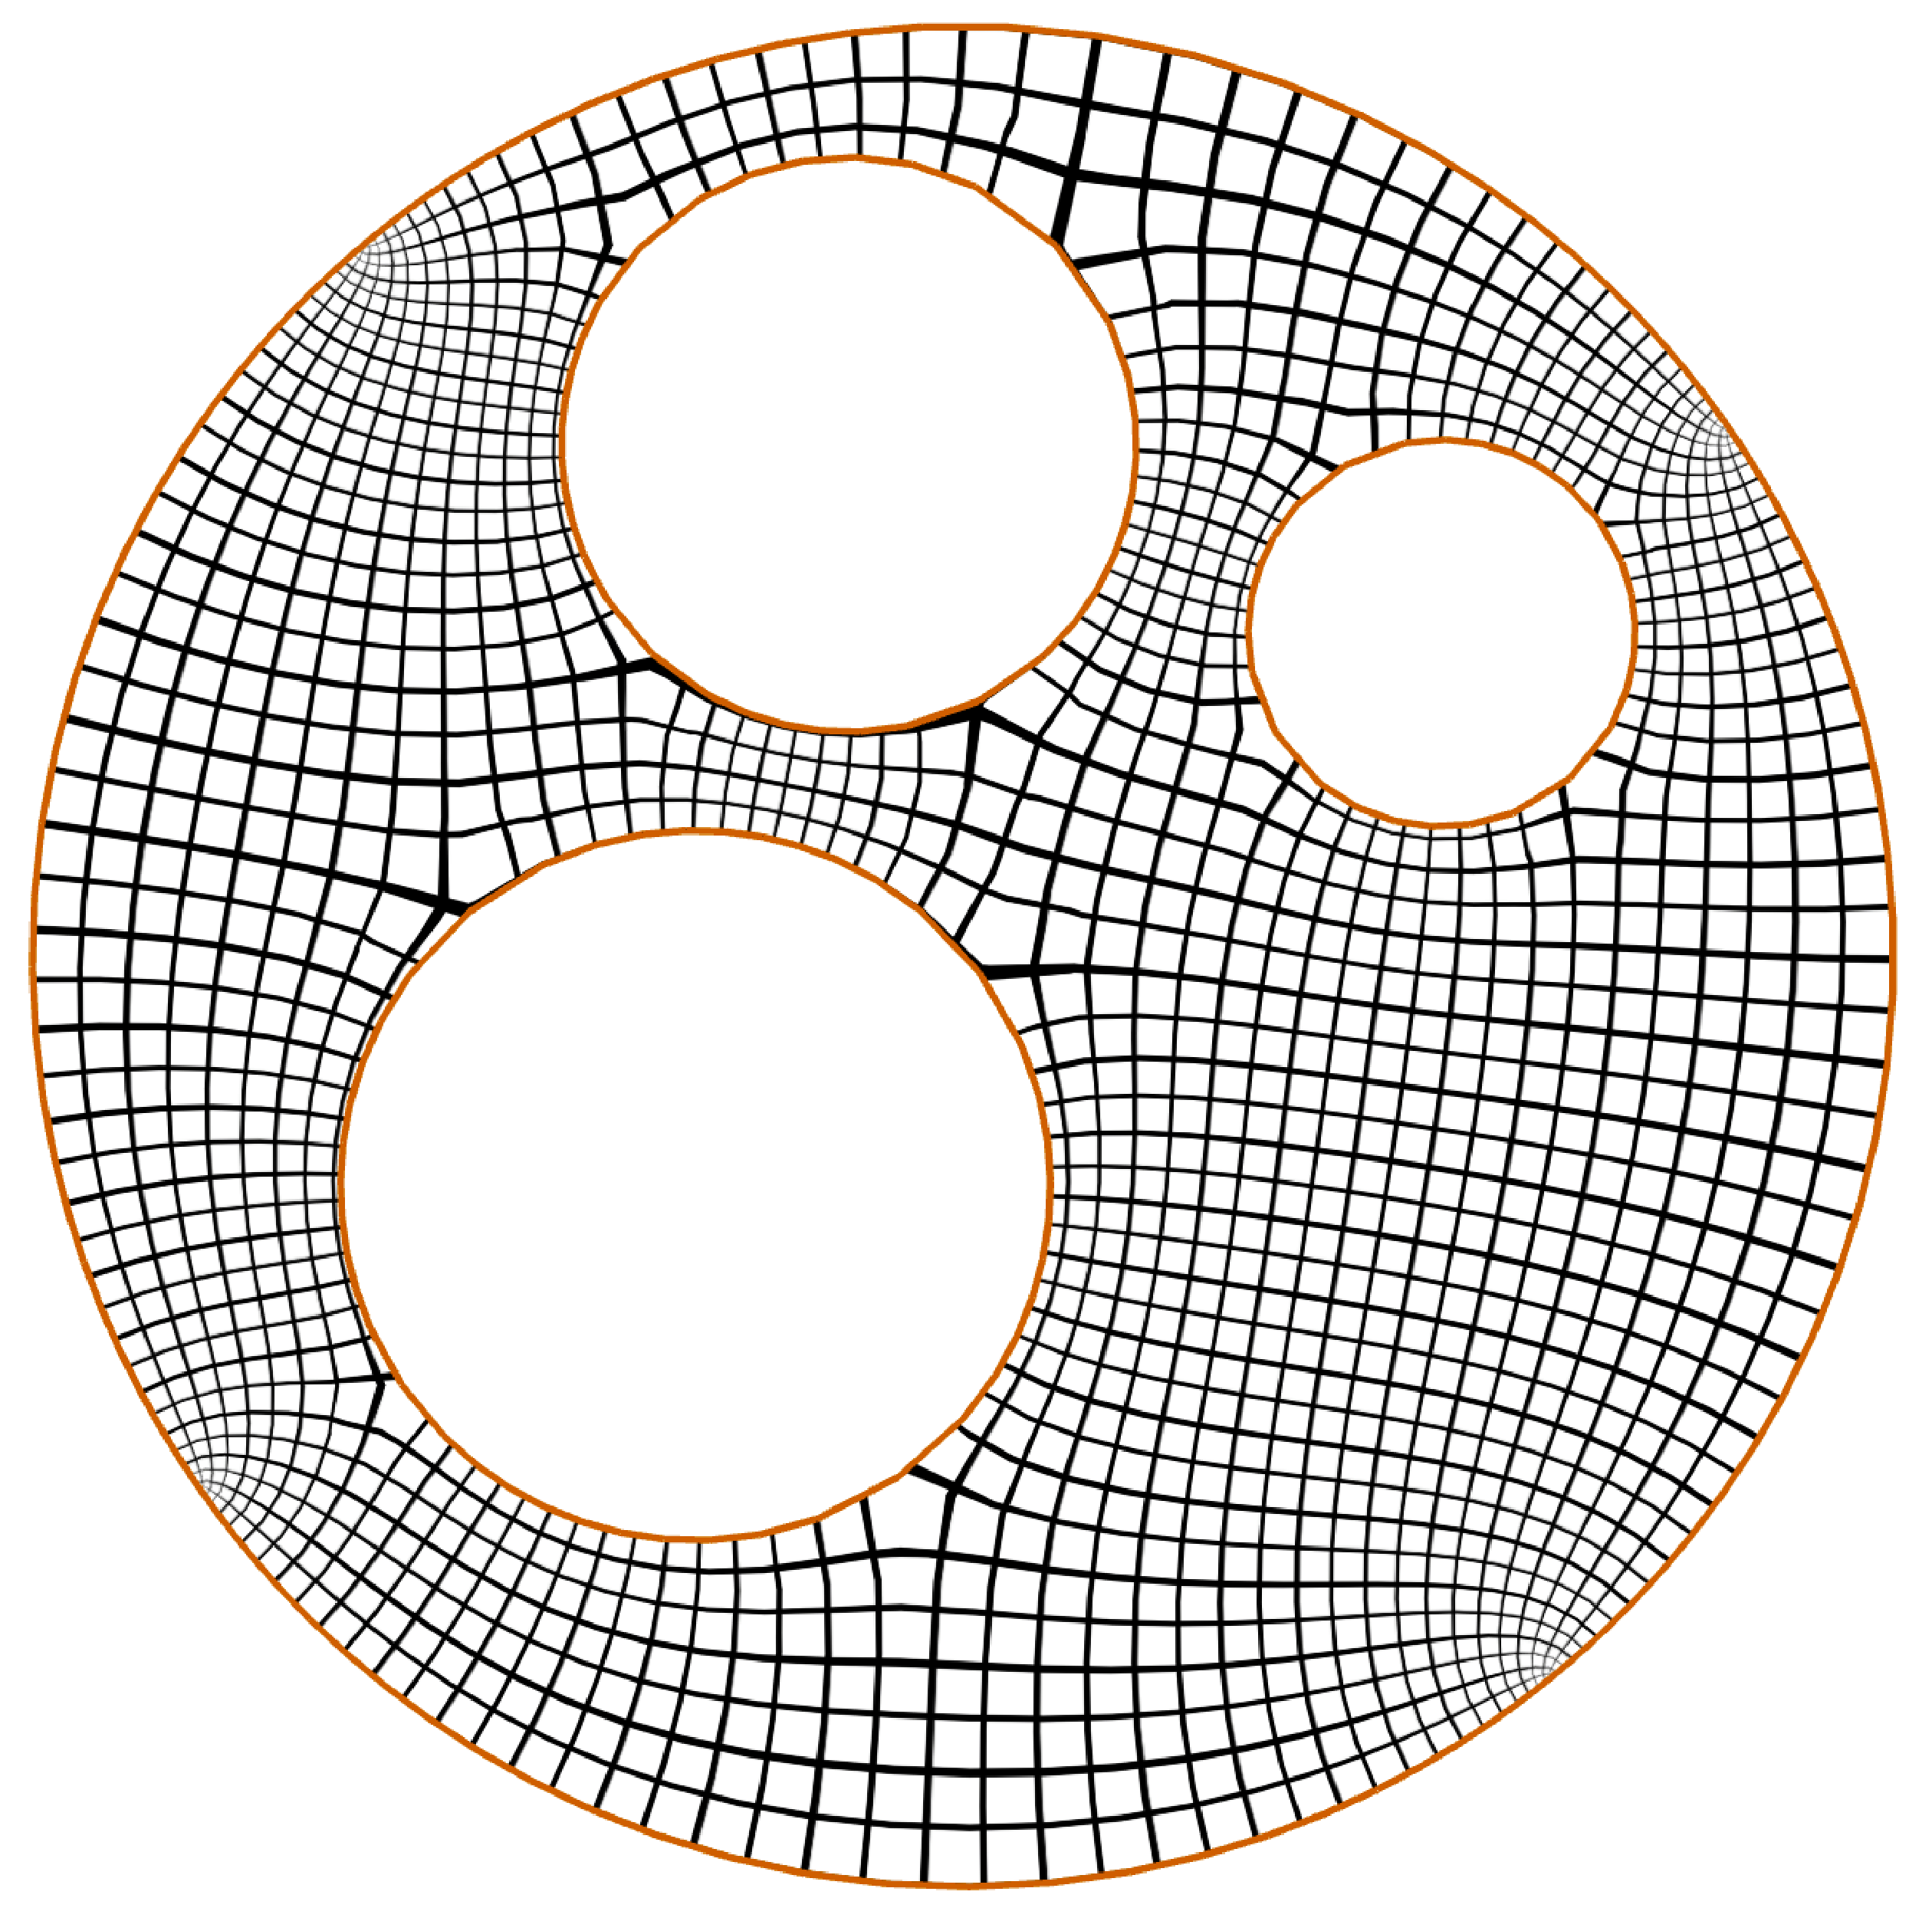
\includegraphics[width=0.5\textwidth]{circle_domain_euclidean/three_holes_map.pdf}
}
\setstretch{0.8}{\scriptsize\tt data/circle\_domain\_euclidean/three\_holes.xml}
\caption{
Discrete conformal map of a multiply-connected domain to a region bounded by circles.
}
\label{fig:euclidean_circle_domain}
\end{figure}

We call a cyclic planar domain a circle domain if the vertices of each boundary component are inscribed in a circle.
In this section we present discrete conformal maps from planar domains to circle domains, see Figure~\ref{fig:euclidean_circle_domain}.
There is an analogous theorem for surfaces with higher genus, see Section~\ref{sec:hyperbolic_circle_domain} and Figure~\ref{fig:hyperbolic_circle_domain}.
In the smooth setting the corresponding theorem has been conjectured by Koebe. 
Every domain in $\C$ is conformally equivalent to a domain bounded by circles.
The process to calculate a discrete map from a discrete planar cyclic domain to a discrete circle domain is as follows.
Suppose there is a unique exterior boundary component. Fill all interior boundary components by attaching faces. 
Triangulate the new faces to produce a set of new edges $E_2$. 
Let $\lambda_{\it ij}$ with $\it ij\in E_2$ be free variables of the mapping problem.
Map the domain to a circle as described in Section~\ref{sec:riemann_map} by solving Problem~\ref{prob:factors_and_angles} with these extra variables.
Remove extra edges $\it ij\in E_2$.
The boundary vertices of the result are inscribed in circles, see Figure~\ref{fig:euclidean_circle_domain}.


\subsection{Special multiply connected domains}

\begin{figure}
	\centering
	\resizebox{\textwidth}{!}{
	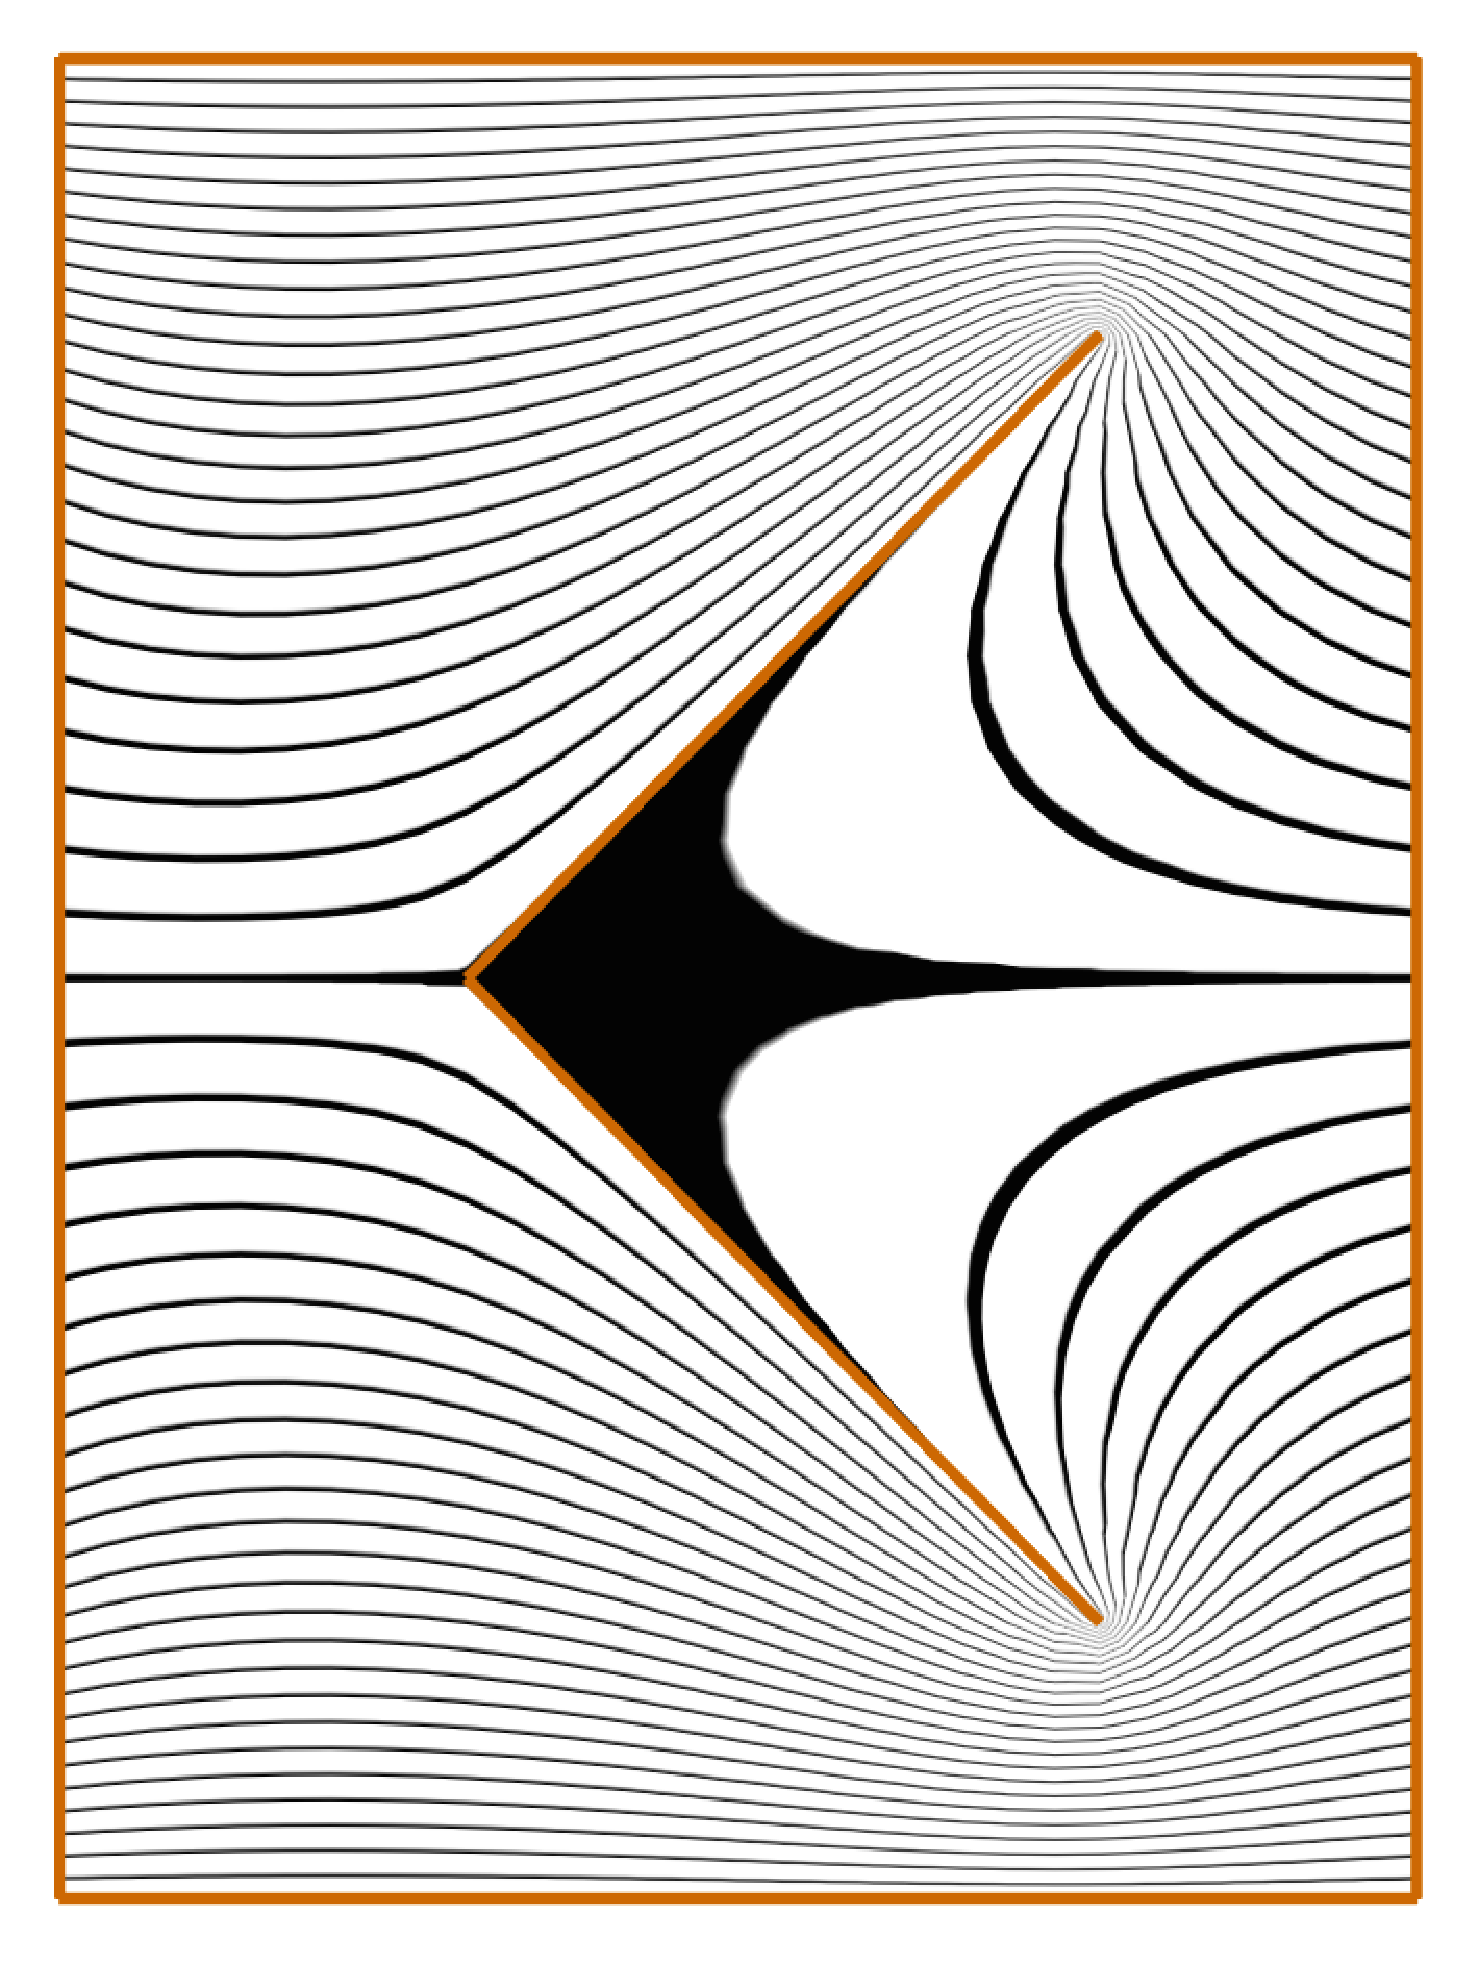
\includegraphics[height=5cm]{planar_streams/arrow_cylinder.pdf}
	\hskip 0.01\textwidth
	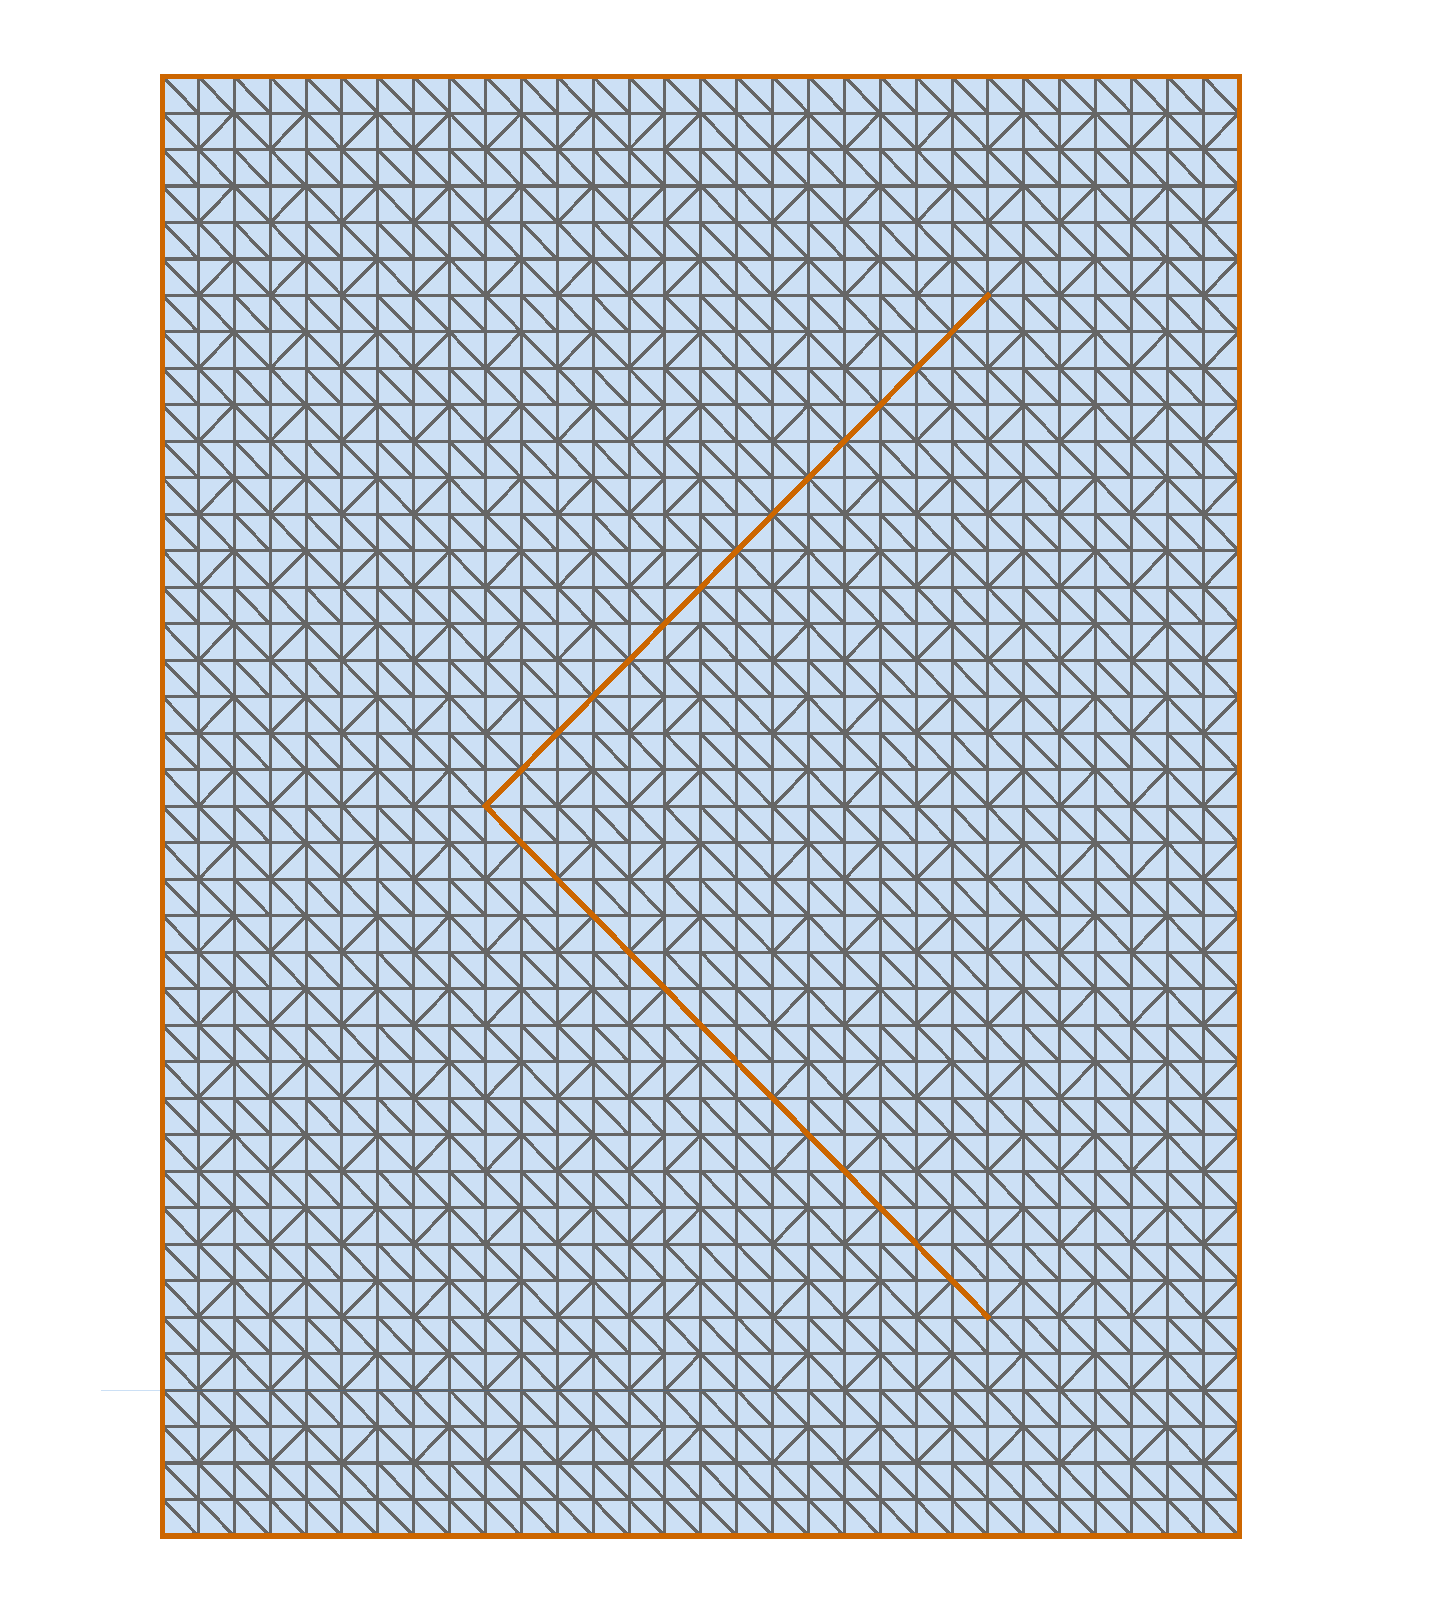
\includegraphics[height=5cm]{planar_streams/arrow_cylinder_image.pdf}\hfill
	\hskip 0.01\textwidth
	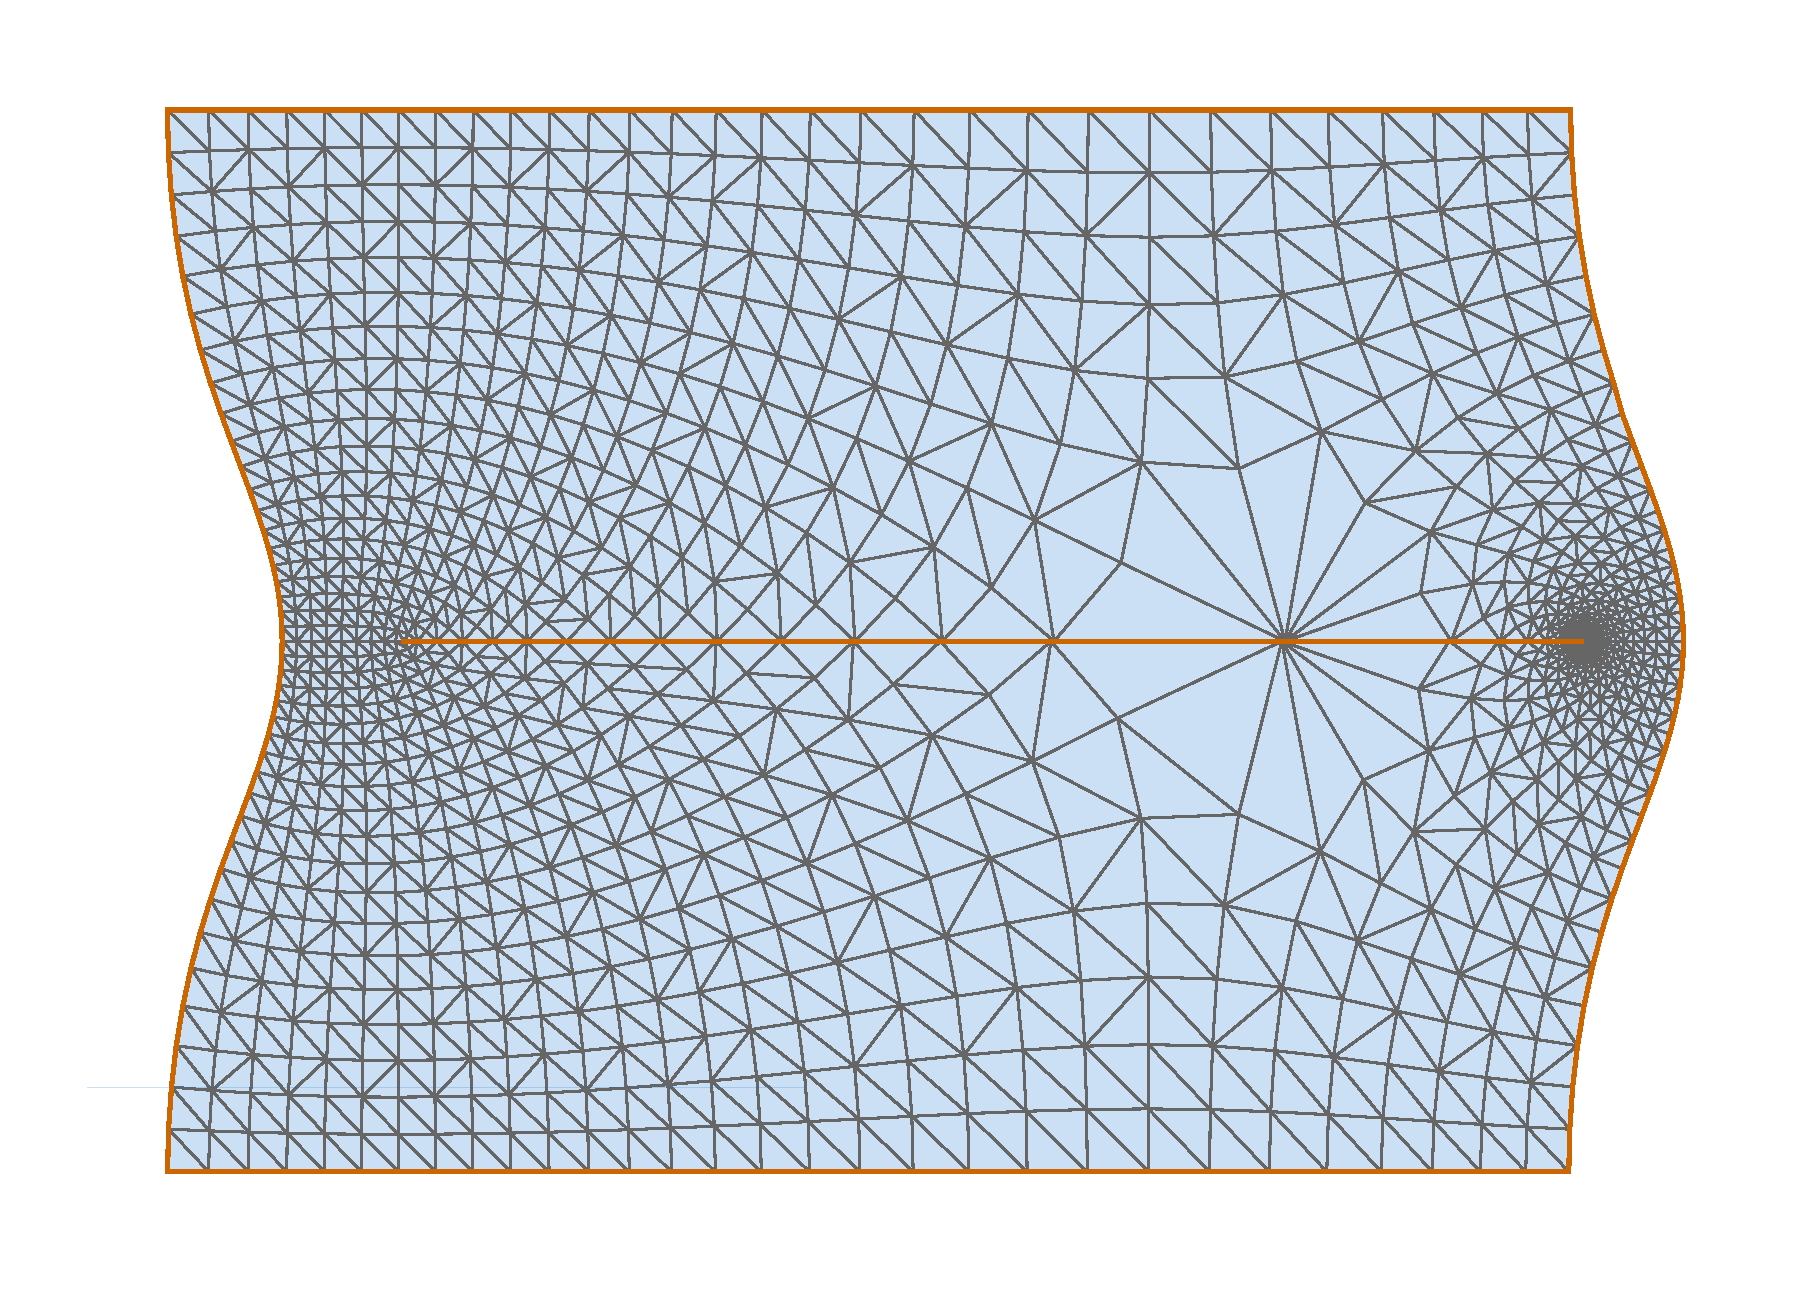
\includegraphics[height=5cm]{planar_streams/arrow_cylinder_domain.pdf}
	}
	\setstretch{0.0}{\scriptsize\tt data/planar\_streams/arrow\_cylinder\_planar.xml}
	\resizebox{\textwidth}{!}{
	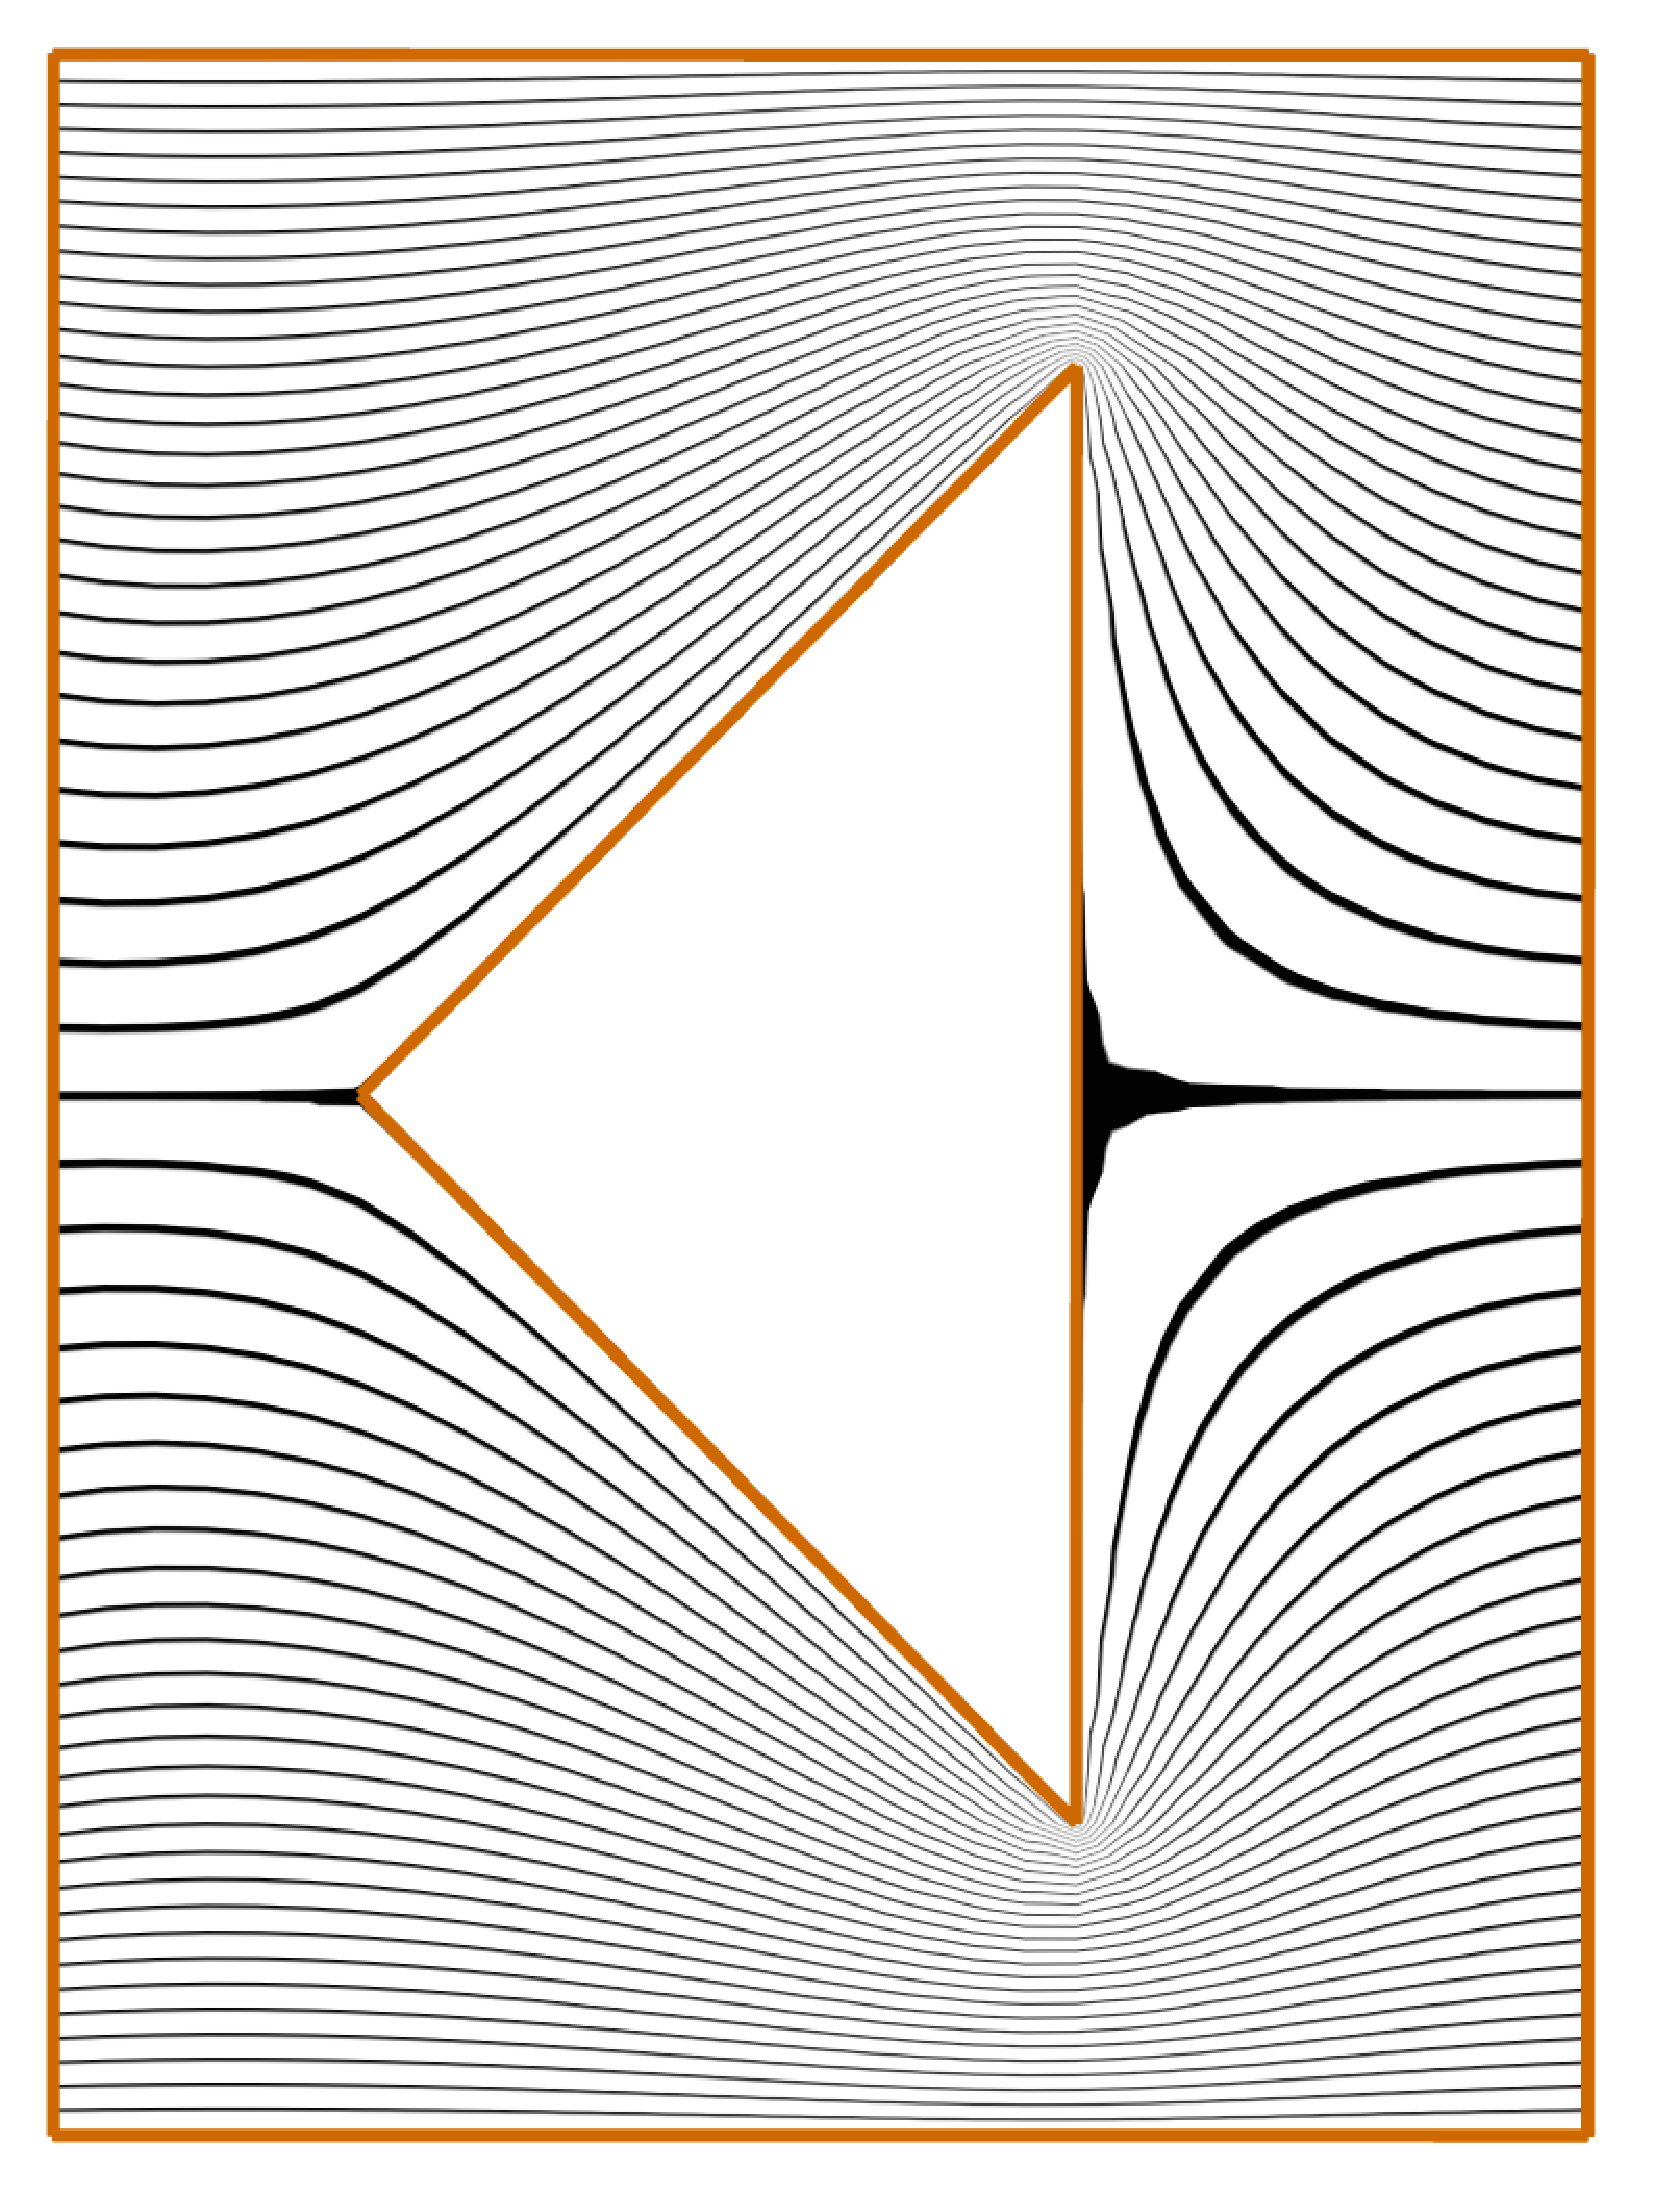
\includegraphics[height=5cm]{planar_streams/triangle_cylinder.pdf}
	\hskip 0.01\textwidth
	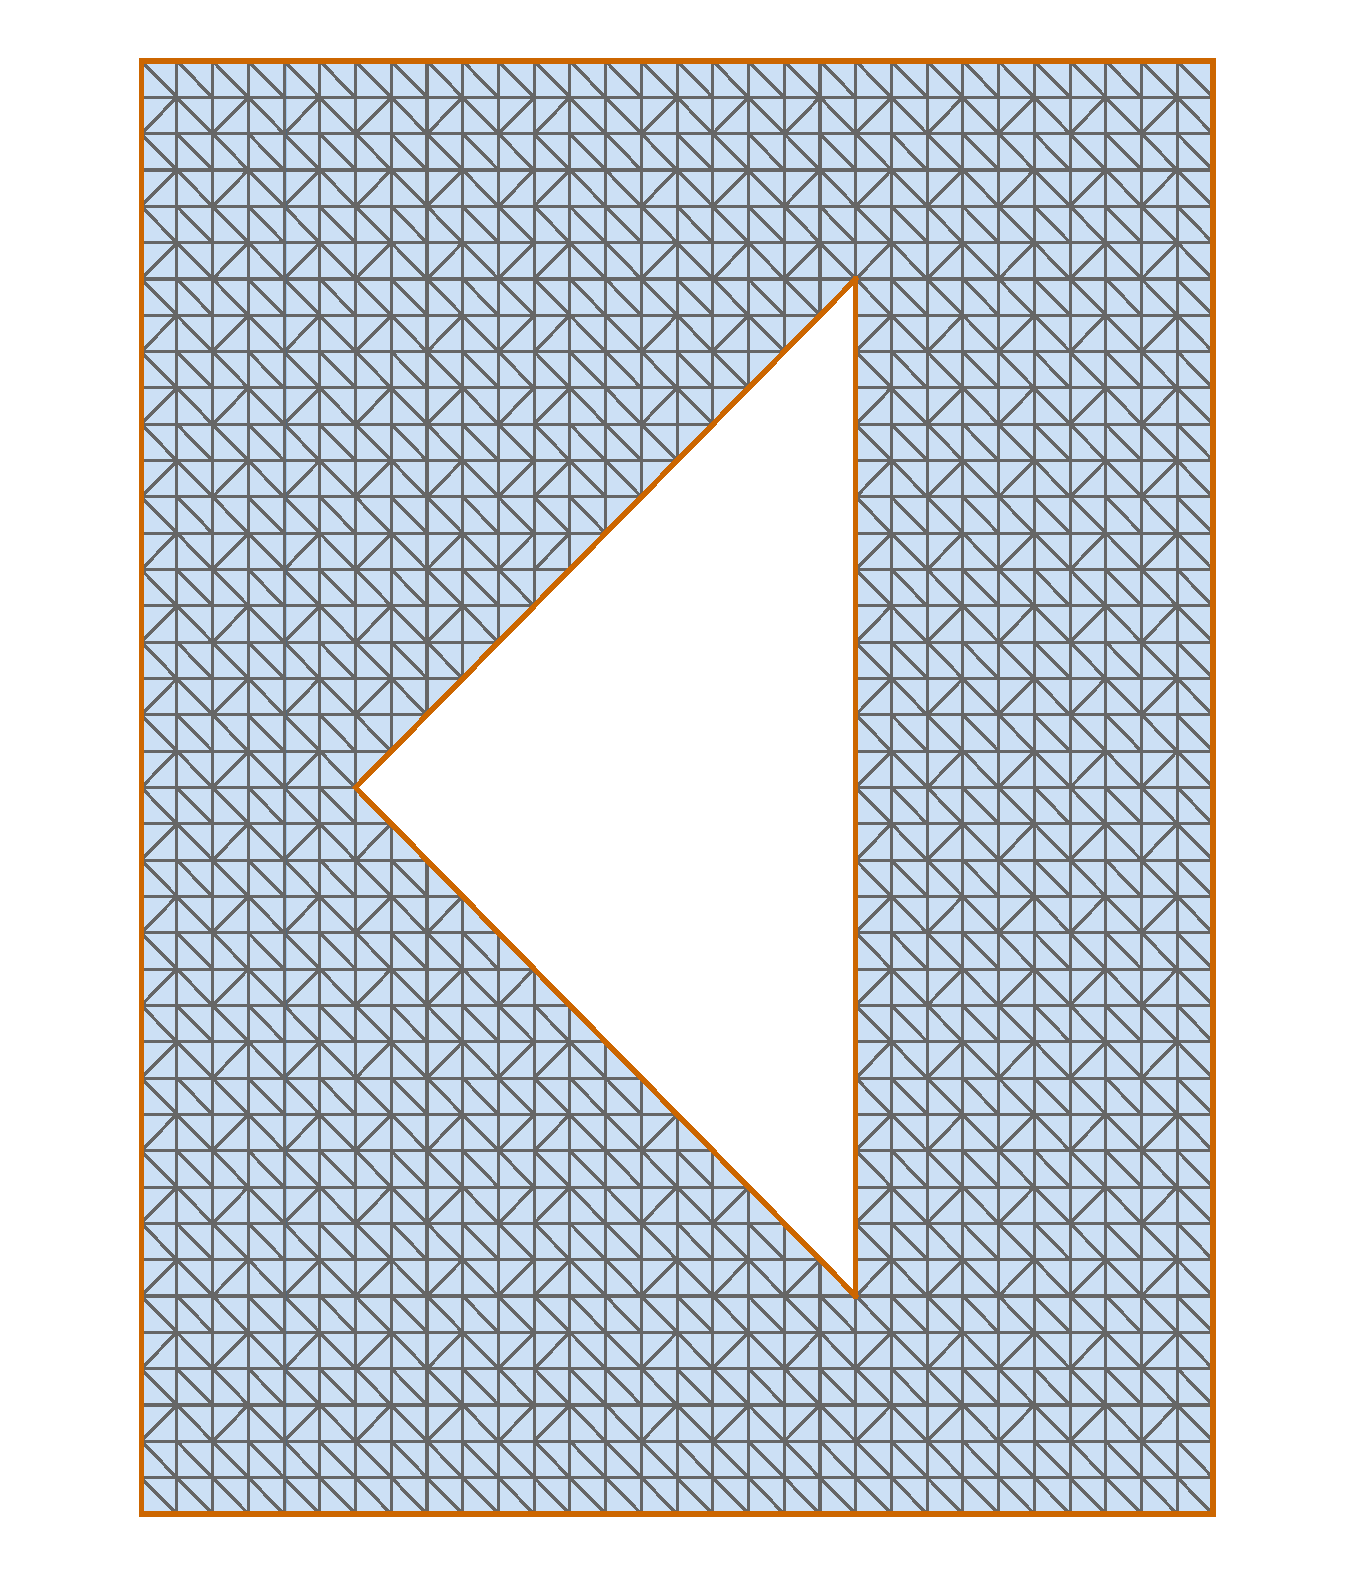
\includegraphics[height=5cm]{planar_streams/triangle_cylinder_image.pdf}\hfill
	\hskip 0.01\textwidth
	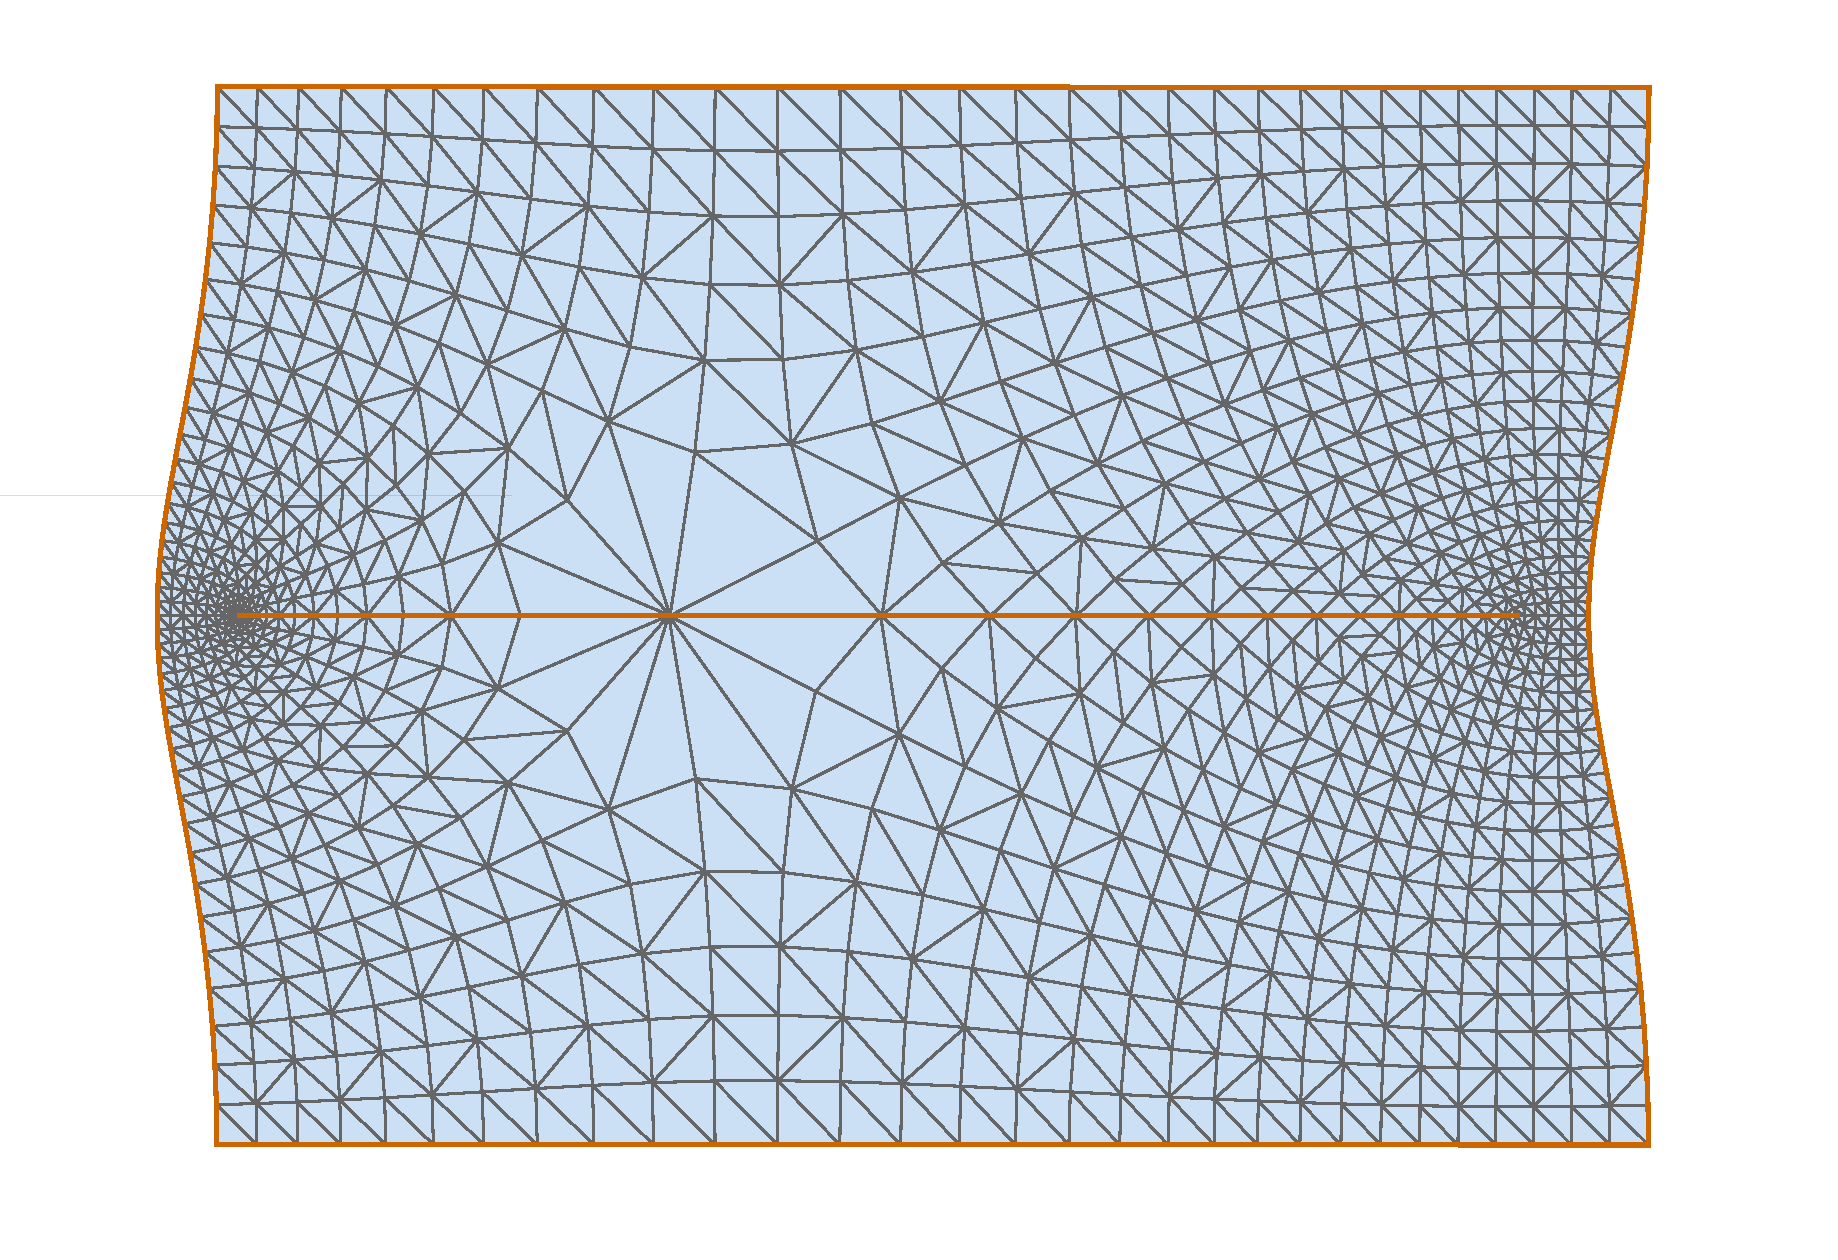
\includegraphics[height=5cm]{planar_streams/triangle_cylinder_domain.pdf}
	}
	\setstretch{0.0}{\scriptsize\tt data/planar\_streams/triangle\_cylinder\_planar.xml}
	\resizebox{\textwidth}{!}{
	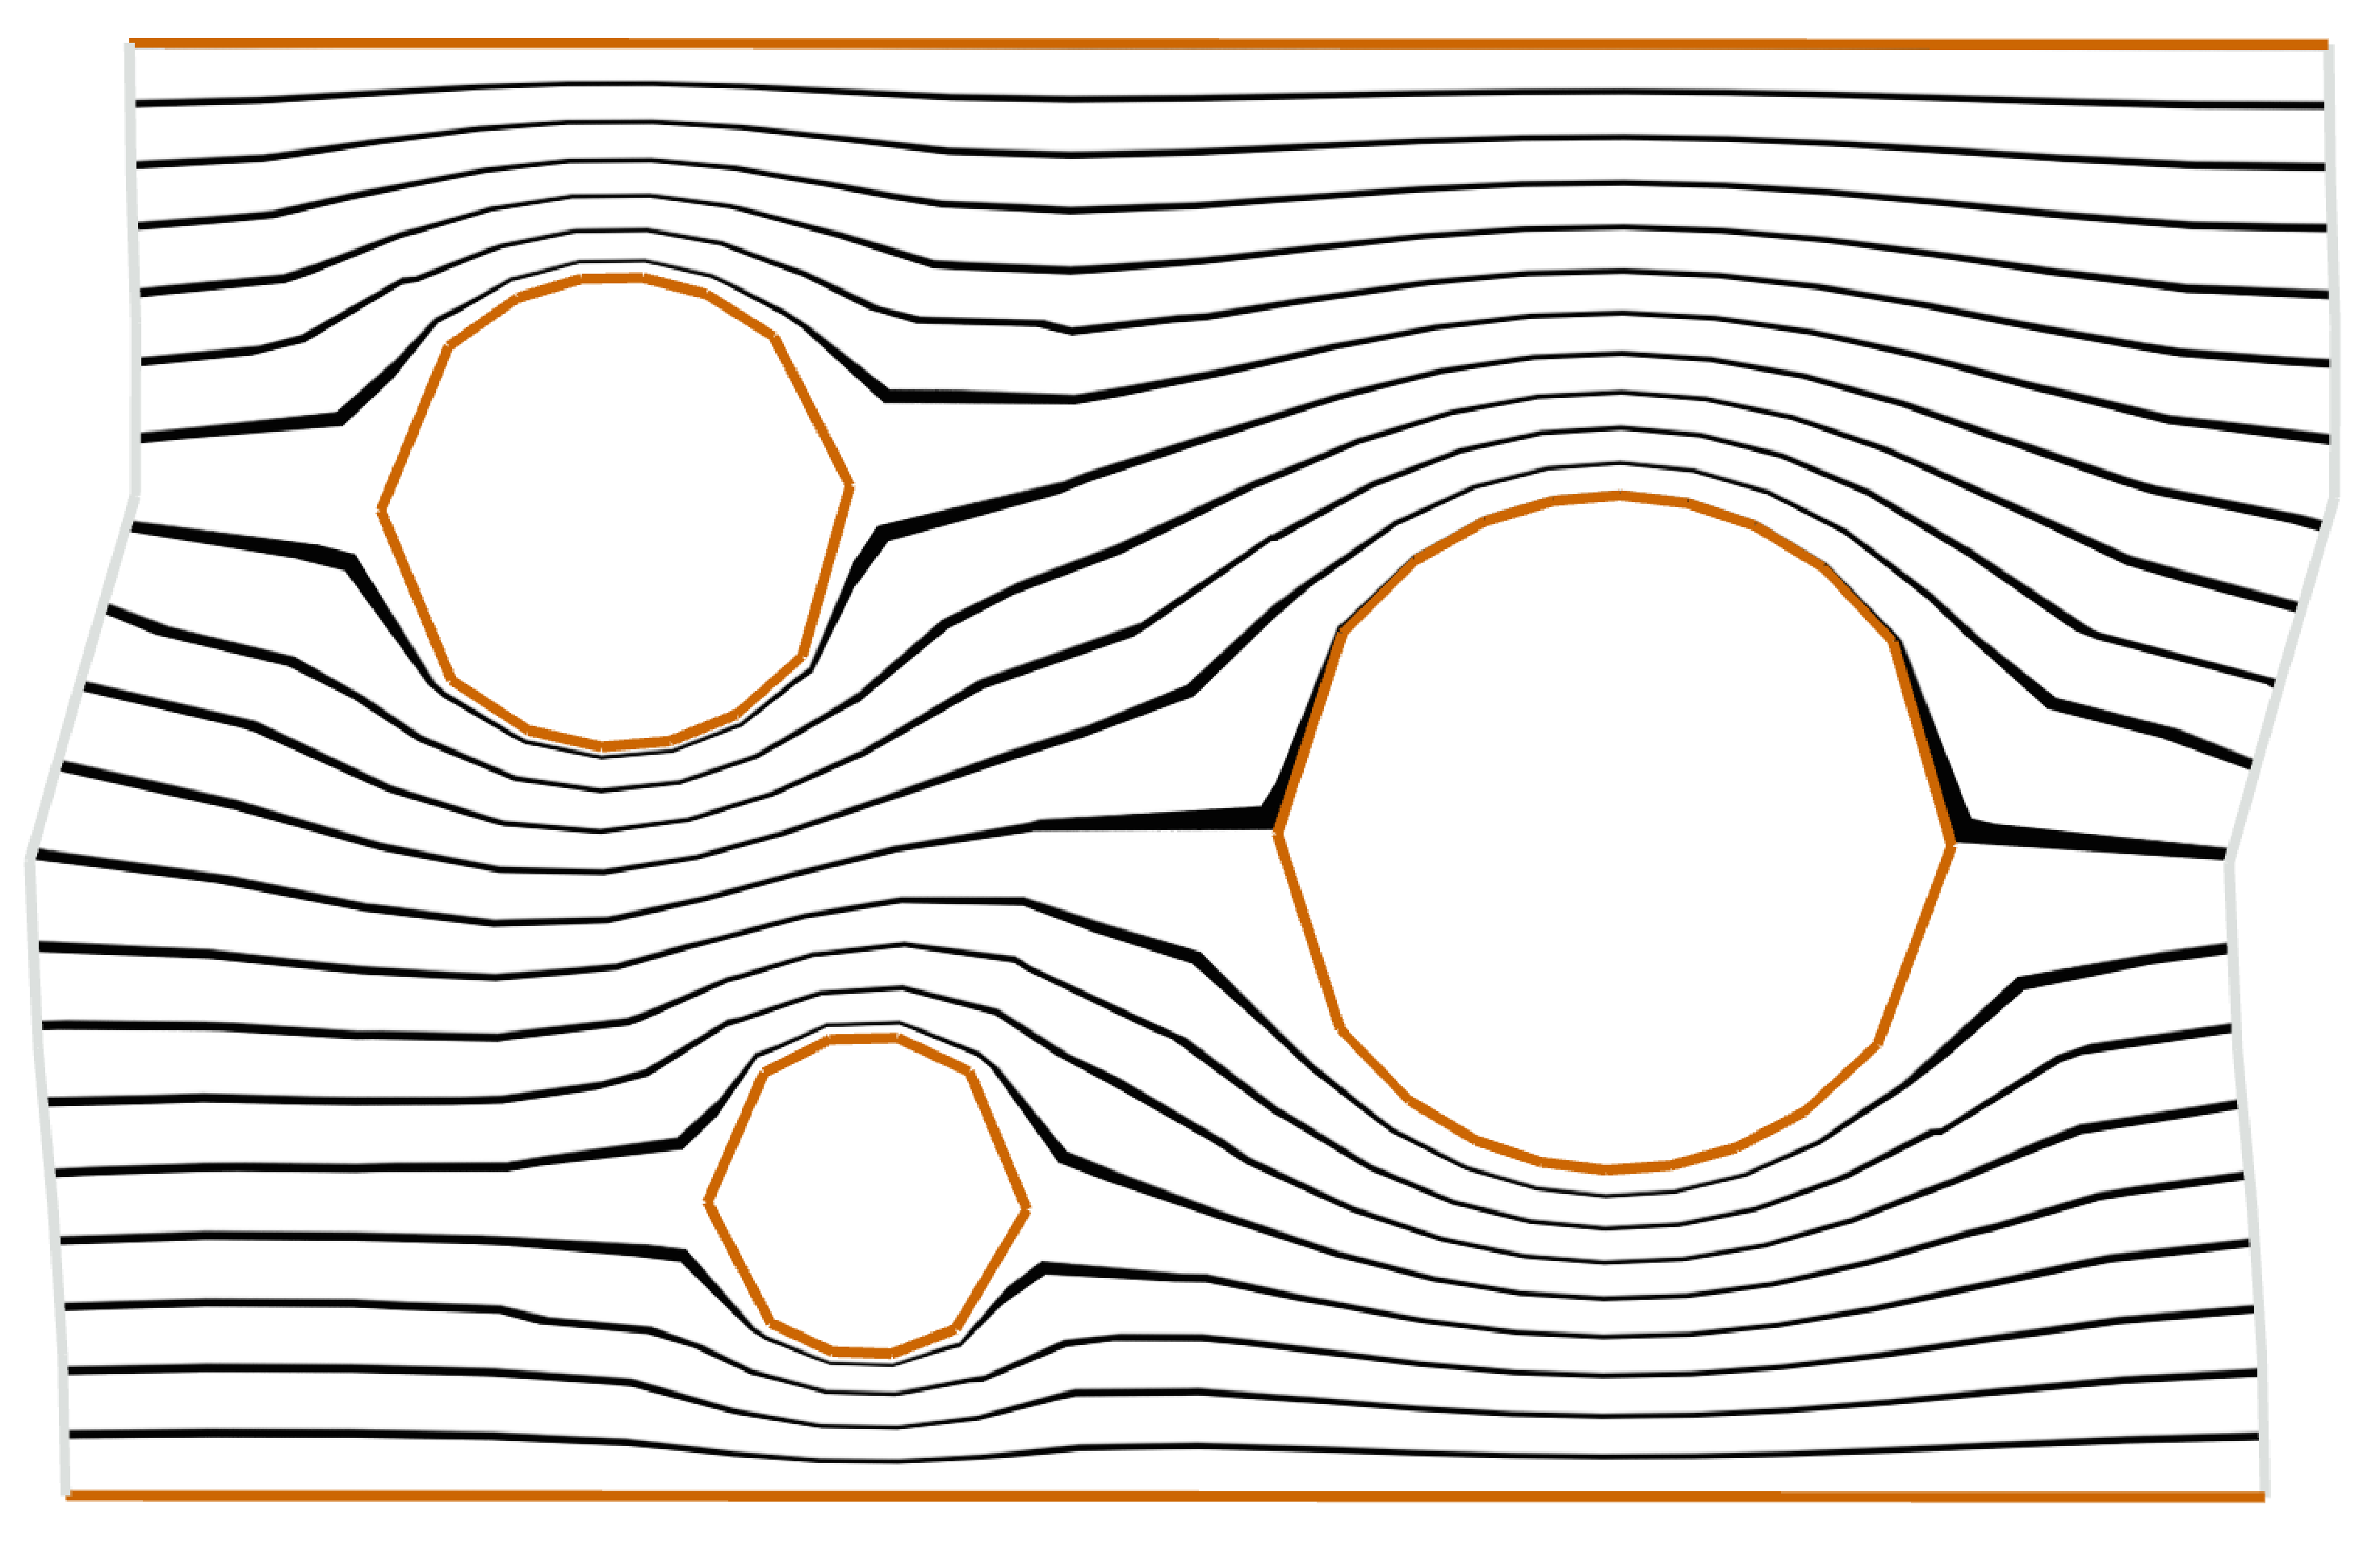
\includegraphics[height=5cm]{planar_streams/circular_stream_03_lines.pdf}
	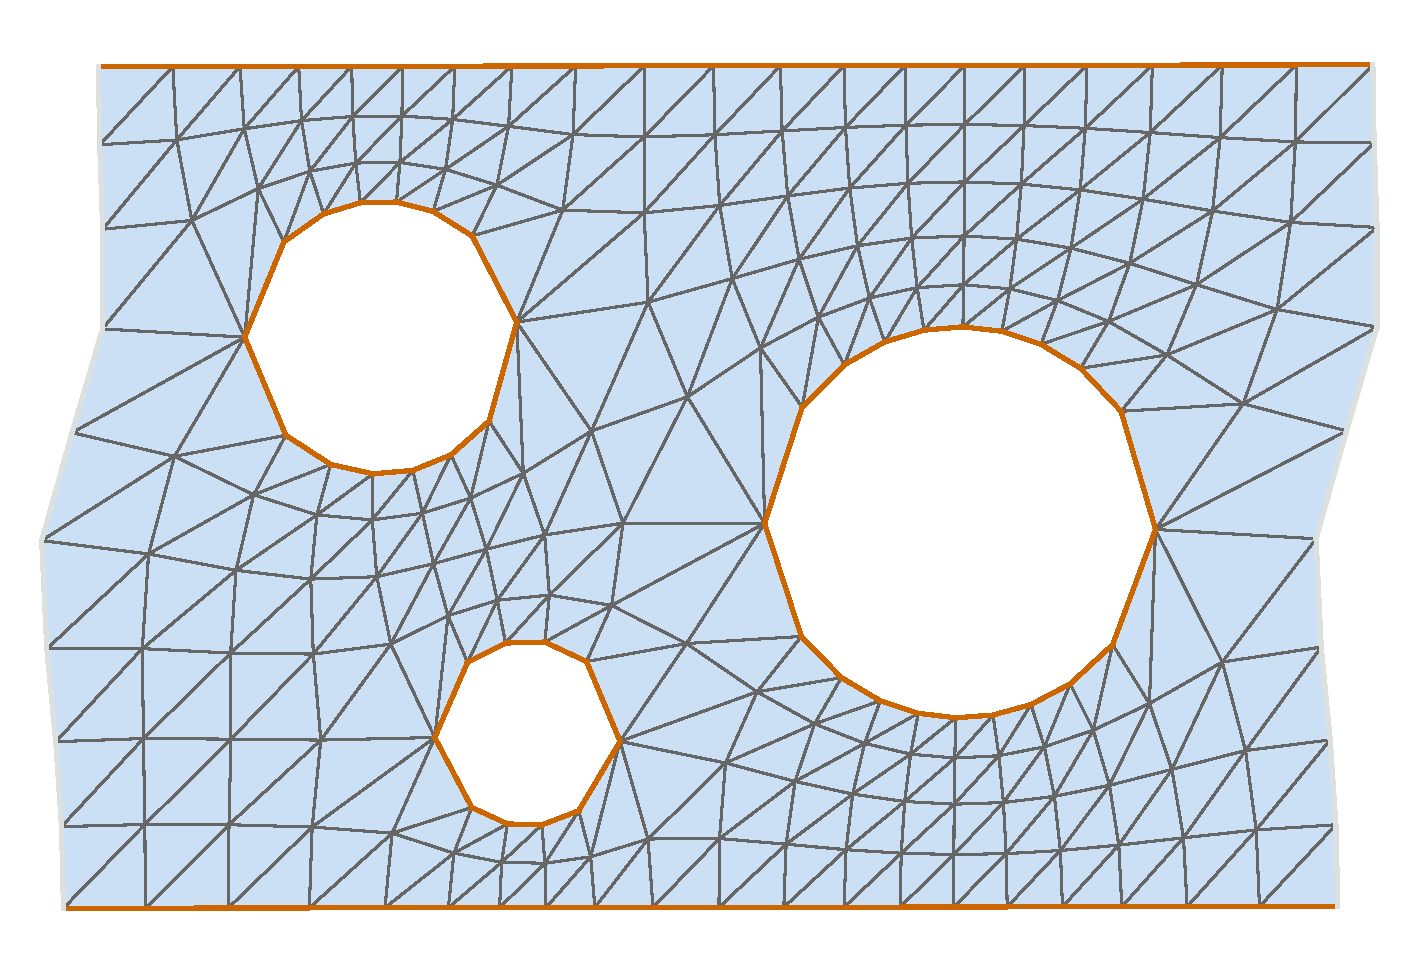
\includegraphics[height=5cm]{planar_streams/circular_stream_03_mesh.pdf}
	}
	\setstretch{0.0}{\scriptsize\tt data/planar\_streams/circular\_stream\_03.xml}
\caption{
Mapping of multiply connected regions.
Conformal map of a topological cylinder with boundary components.
In all images the vertical boundaries are identified.
The boundary of the domain consists of the upper and lower boundary loops and a slit in the interior of the domain.
This can be interpreted as modeling a stream of incompressible fluid flowing around an obstacle with periodic boundary conditions.
\\
Top: Map from an arrow shaped slit to a horizontal slit with straight boundary conditions on the upper and lower boundary loops.
The point on the left of the arrow tip is mapped to the left end of the horizontal slit.
The point on the right side is mapped to the right end.
\\
Middle: Same setup as above using a triangle as third boundary component.
Note that by symmetry the upper and lower corner of the triangle are mapped to the same point in the image of the map.
\\
Bottom: Three circular boundary components are mapped to horizontal slits.
}
\label{fig:fluid_flows}
\end{figure}

In this section we show how to conformally map multiply connected planar domains.
Our examples are inspired by planar potential flows with periodic boundary conditions, see Figure~\ref{fig:fluid_flows}.
The basic idea is to map a given domain with boundary components to periodic region with parallel slits.
We do not solve the general problem of discretely mapping an arbitrary region to a domain with parallel slits here but provide a few examples where we could obtain nice results using discrete conformal mappings as defined above.

In general the main challenge for the computation of such a map is to find the points on the boundary components that map to the ends of the slits. As these points may even not be located at vertices of the underlying mesh in general this involves a mesh refinement procedure. To solve the problem for the general case one would also have to solve an optimization problem to find the location of the points such that the slits become parallel and are oriented in a prescribed direction.

In the first two examples we can derive the pre-images of the slit ends by symmetry. 
We take a rectangle with two identified sides, i.e. a part of a topological cylinder and place a symmetric cut in the shape of an arrow, see Figure~\ref{fig:fluid_flows} upper-left. 
By symmetry the vertices to the left and to the right of the arrow tip get mapped to the ends of the slits. 
This implies that we want to calculate a symmetric flow with respect to the configuration.
The boundary conditions are trivial. 
All $\theta_i$ at the boundary are equal to $\pi$ except for the vertices at the tip of the arrow where $\theta$ is equal to $2\pi$.
In the second example we cut a symmetric triangle to form a boundary component. The pre-images of the slit ends are the left corner of the triangle and the mid-point of the right side, see Figure~\ref{fig:fluid_flows} middle row.

The third example is different from the other two as we inverse the direction of calculation. 
The goal is to create a map from a domain with round holes to a region with parallel slits, see Figure~\ref{fig:fluid_flows} bottom row. 
As we do not want to solve the global optimization problem for the location of the pre-images of slit ends we use a simple trick.
We start with a cylinder with parallel slits.
We add additional edges to triangulate the slits with the condition that none of the edges has zero length.
Remember that the functional is linearly extended to triangulations with angles greater or equal than $\pi$.
We treat the additional edges as auxiliary edges in a circular polygon, i.e., the corresponding $\lambda$s in the functional are variables of the optimization. 
Thus adjacent triangles form a circular polygon in the resulting image.

\section{Uniformization of spheres}
\label{sec:spheres}

In this section we describe how to calculate discrete conformal maps to the sphere.
In Section~\ref{sec:spheres_euclidean} we use a similar construction as for the Riemann map to treat meshes without boundary using the euclidean functional.
As the corresponding spherical version of the variational principle is non-convex it is numerically difficult to find direct solutions.
If we want to state boundary conditions we however cannot avoid using the spherical version.
We describe how we proceed with the spherical functional in Section~\ref{sec:spherical_computation}.

\subsection{Uniformization with euclidean functional}
\label{sec:spheres_euclidean}

\begin{figure}
\centering
\resizebox{0.7\textwidth}{!}{
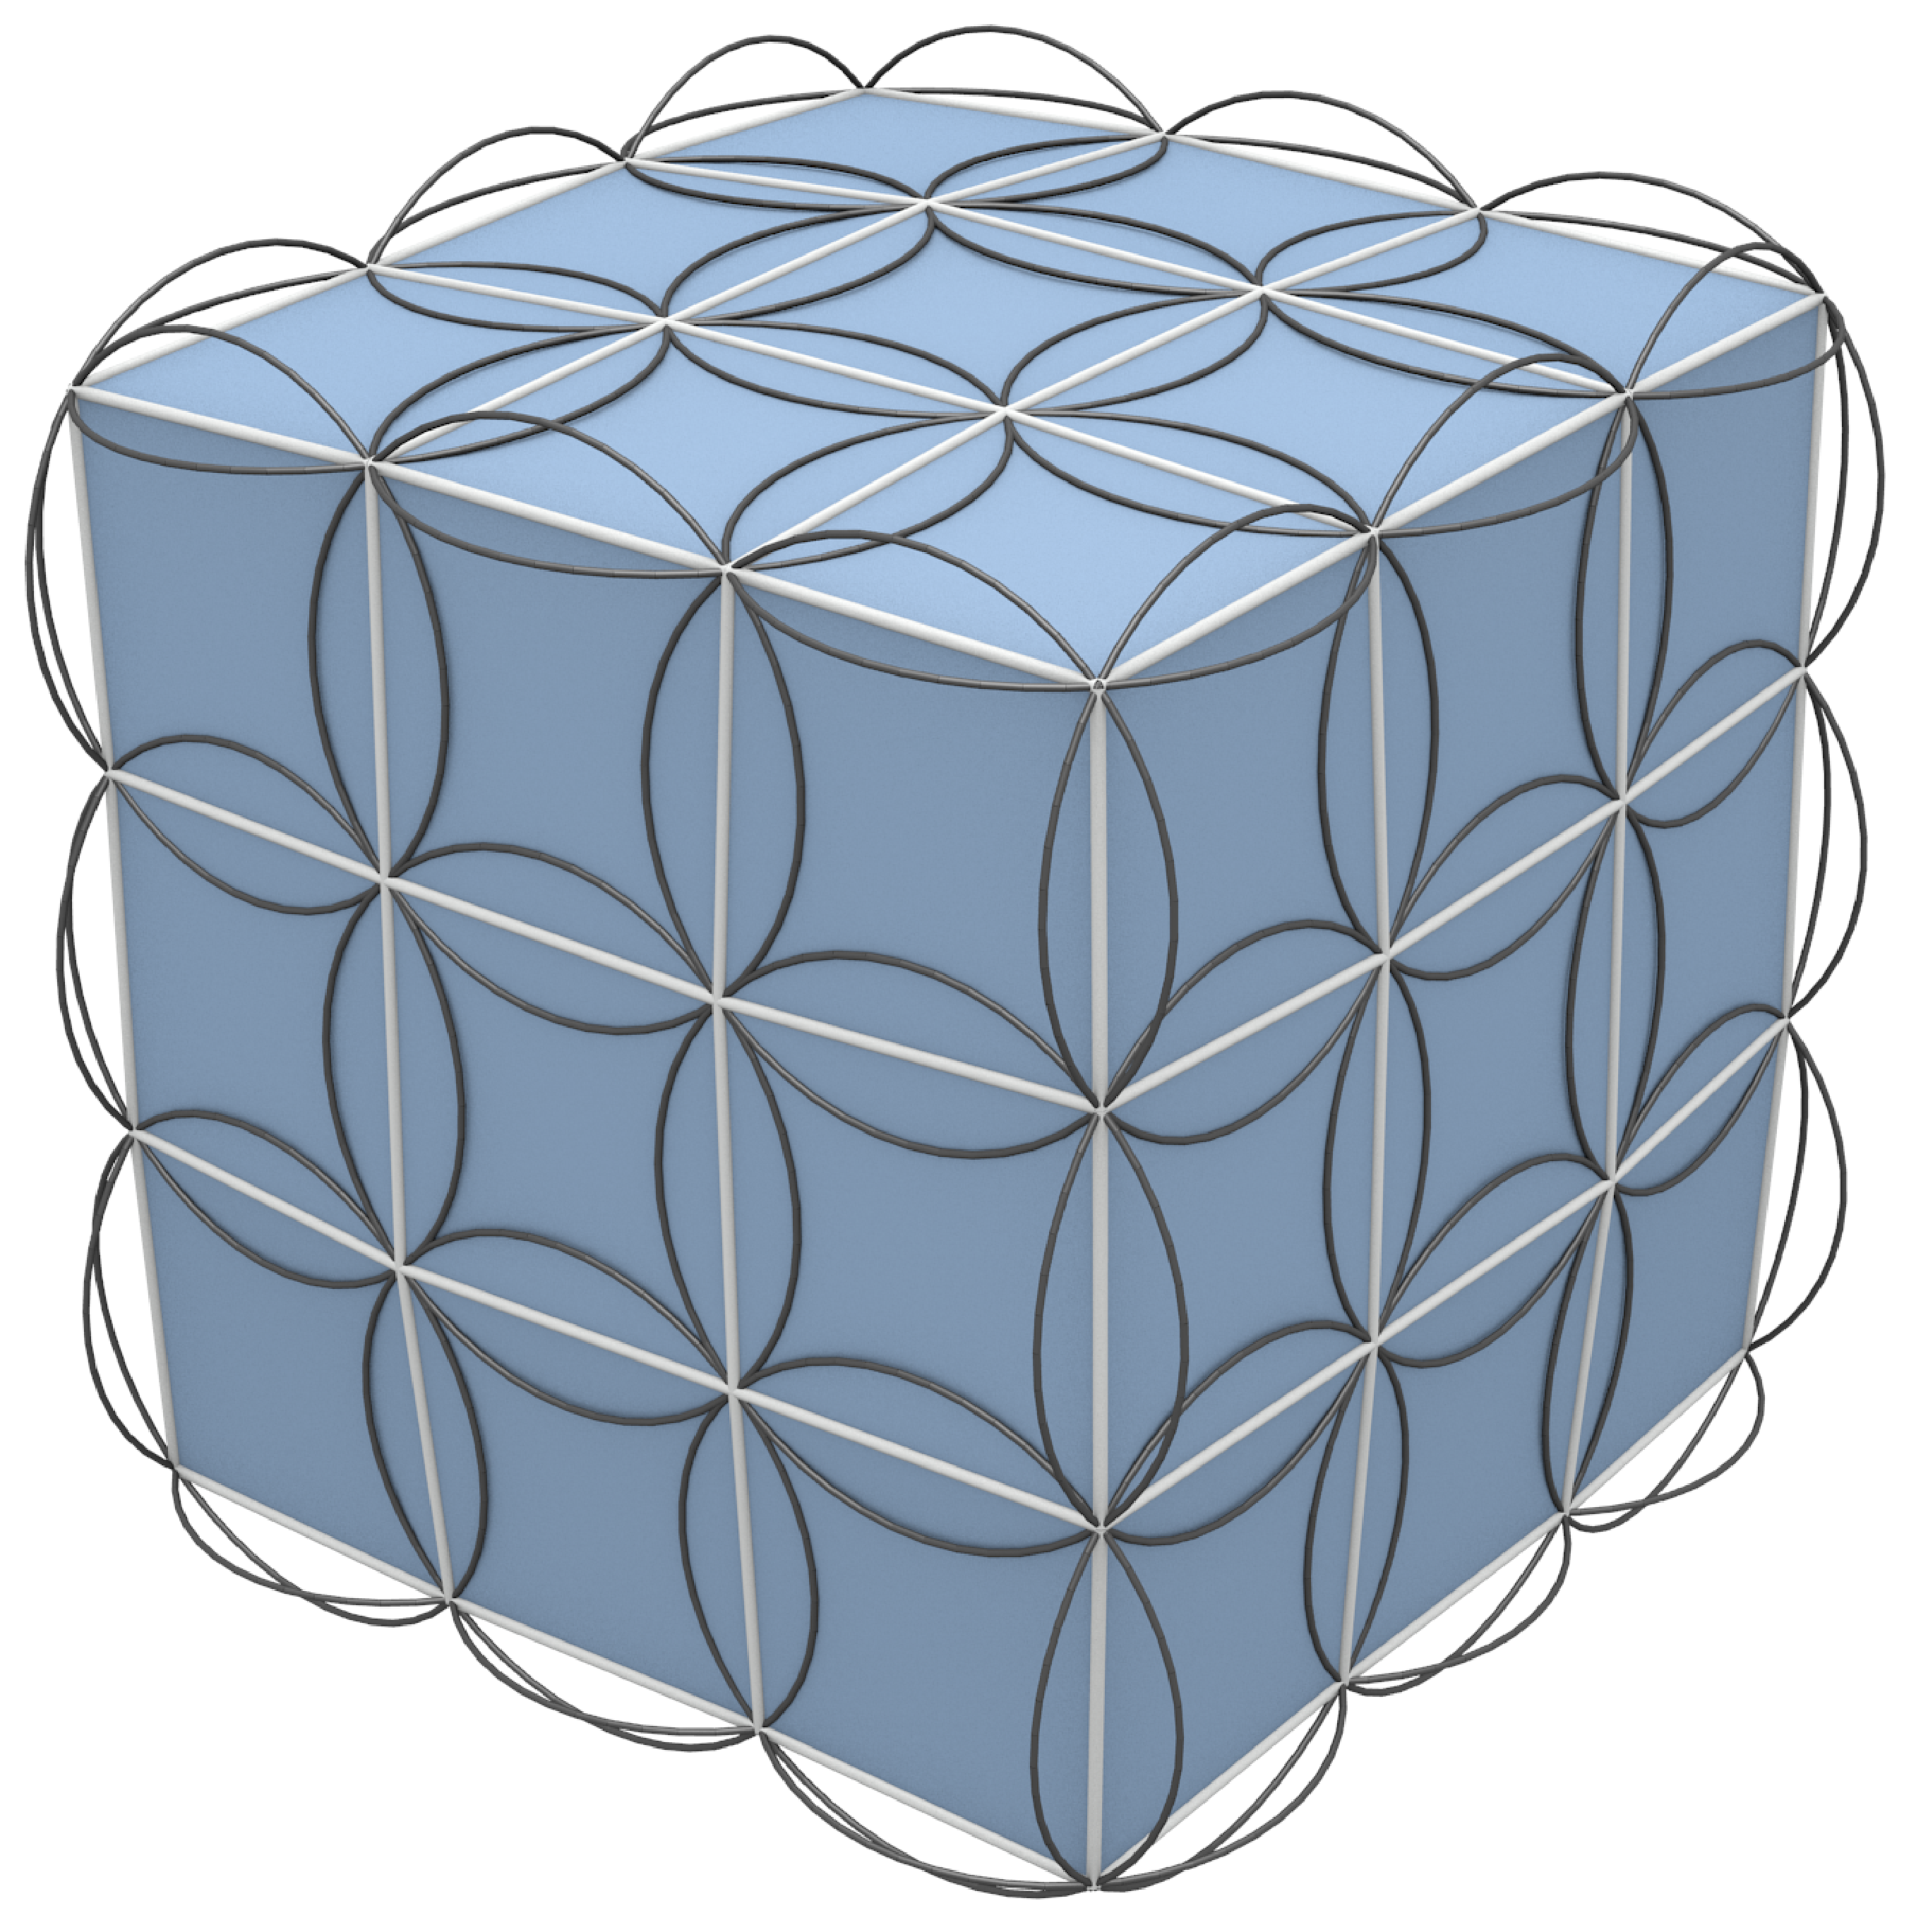
\includegraphics[height=5cm]{spherical_cyclic/cube_cyclic_domain.pdf}
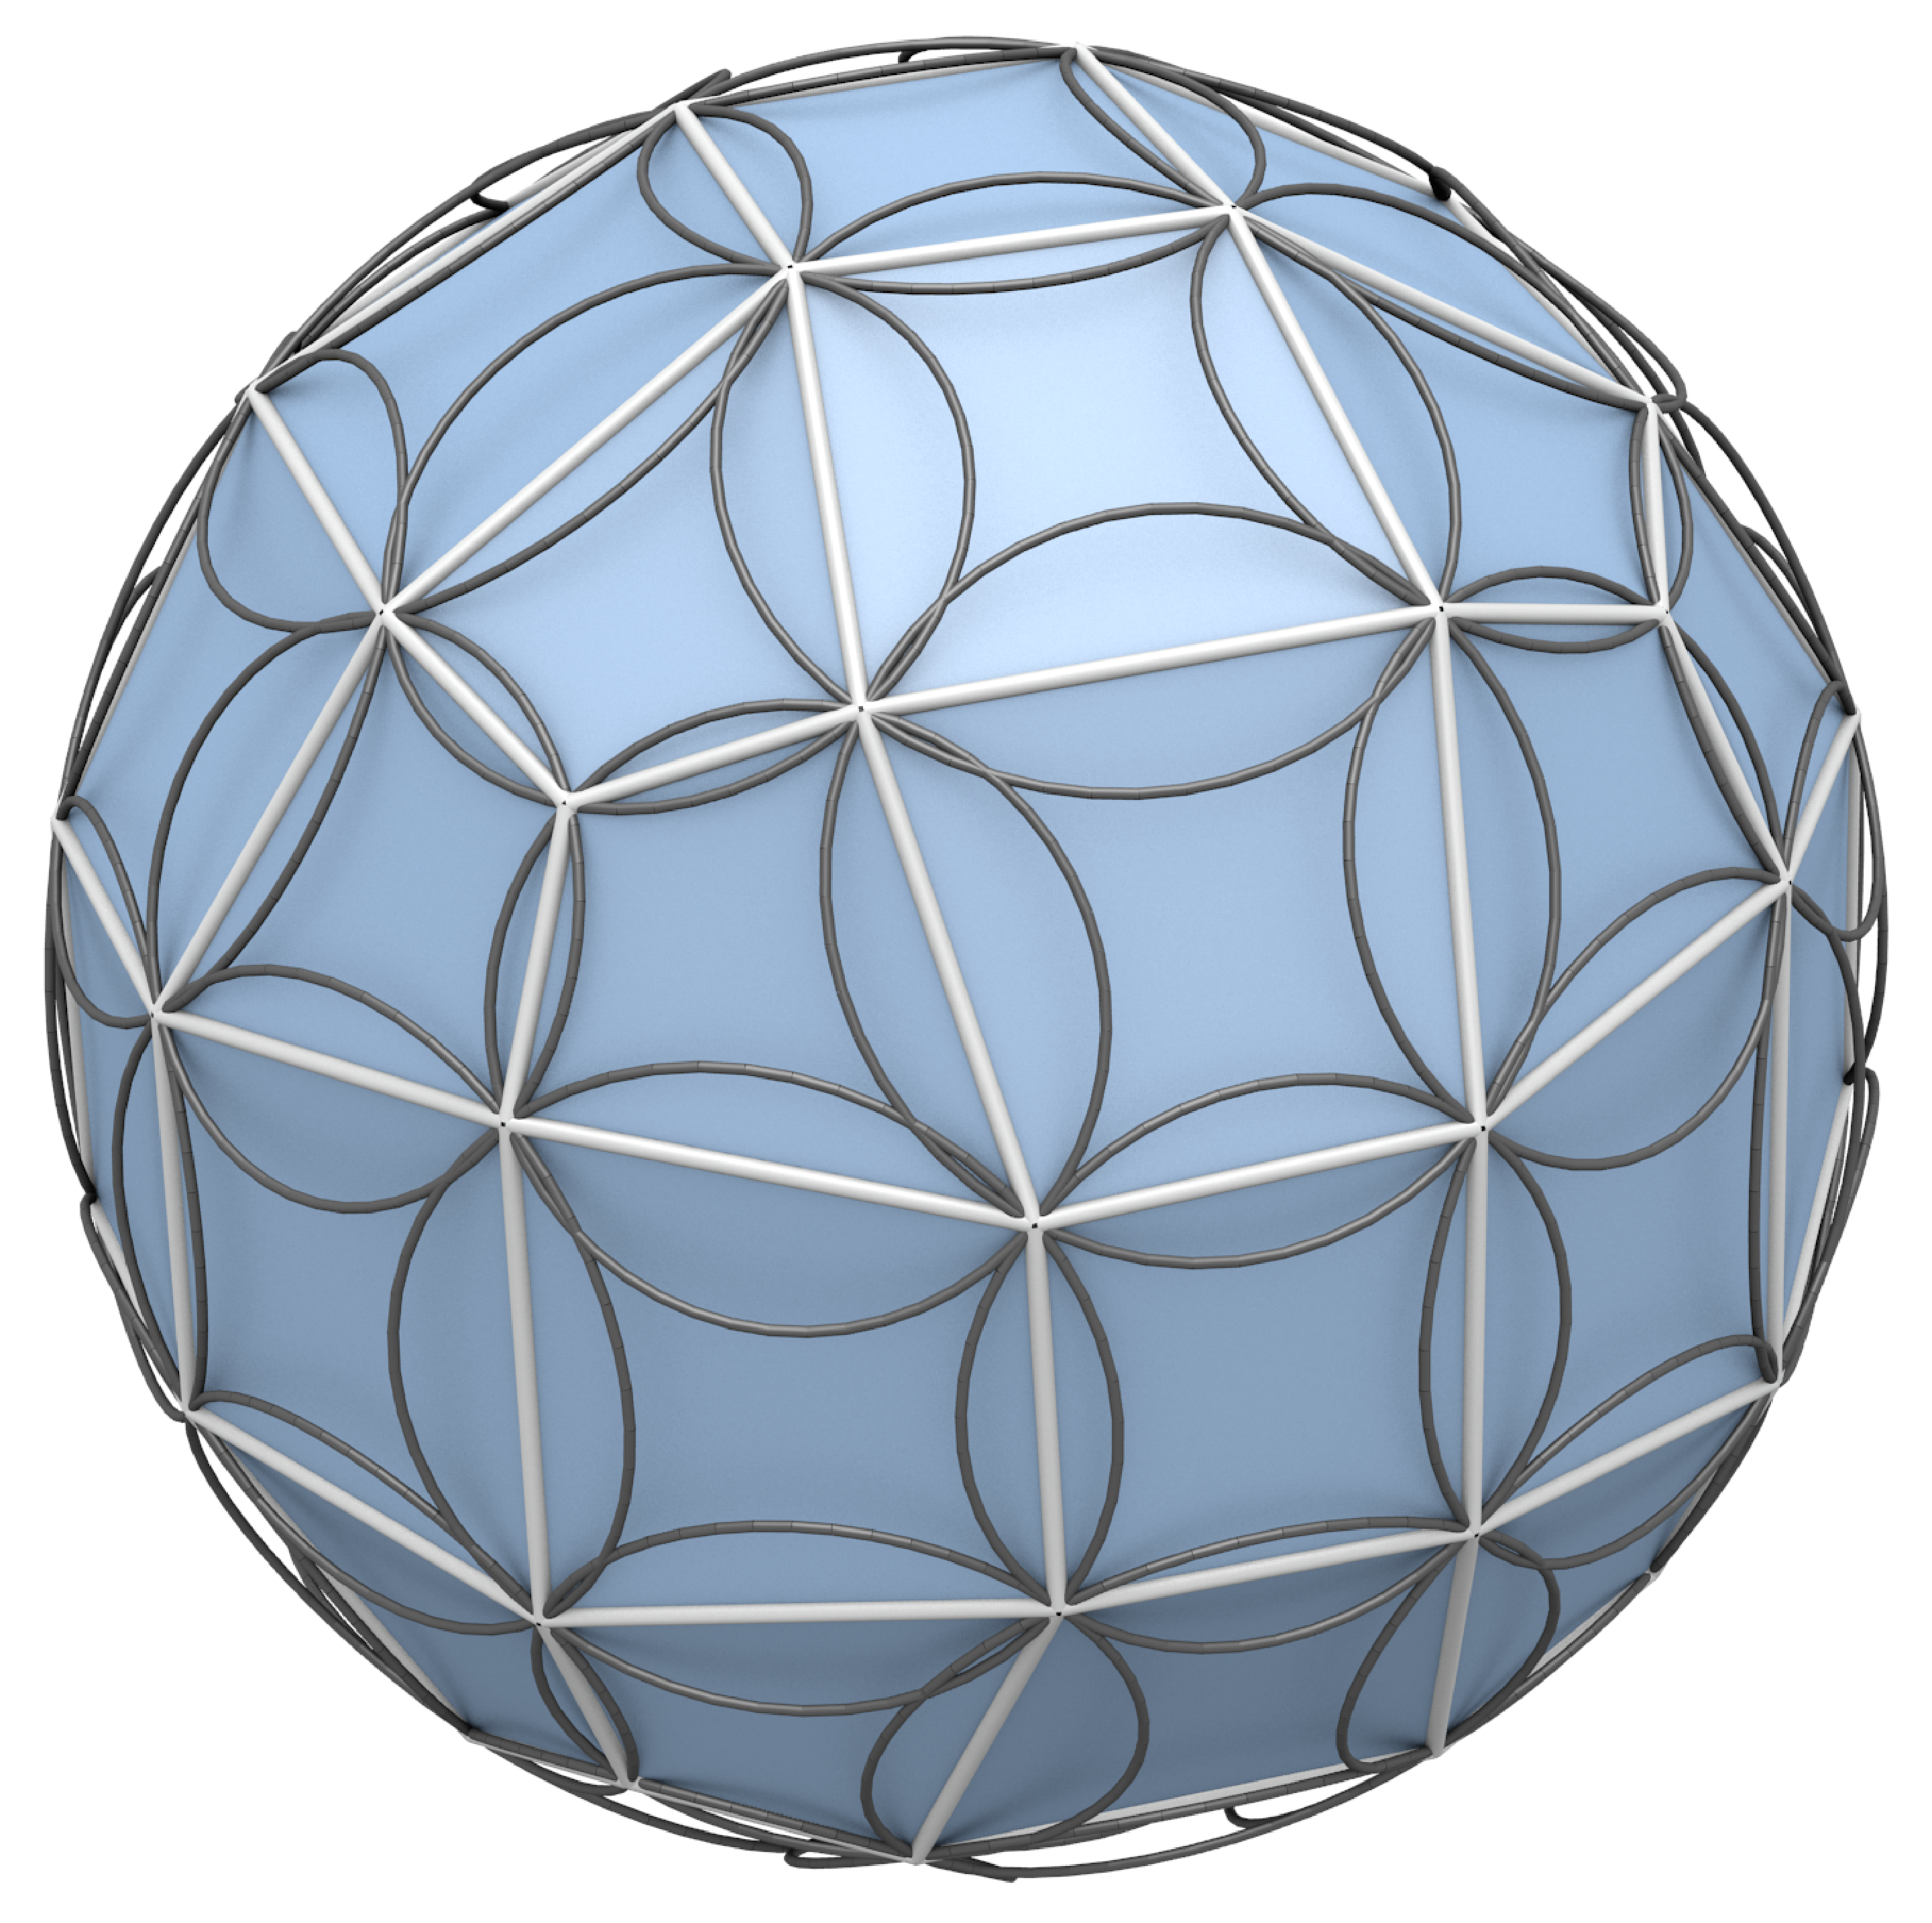
\includegraphics[height=4.8cm]{spherical_cyclic/cube_cyclic_image.pdf}
}
\setstretch{0.0}{\scriptsize\tt data/spherical\_cyclic/spherical\_circular.xml}
\caption{
Discrete cyclic conformal map to the sphere. 
The map was calculated with the euclidean functional and stereographic projection.
We apply M{\"o}bius normalization to the spherical surface to achieve the symmetry
}
\label{fig:spherical_circular}
\end{figure}

Mapping a discrete cyclic surface with spherical topology to discretely conformally the round sphere can be achieved with a similar procedure as described in Section~\ref{sec:riemann_map}. 
We treat the special case of a quad surface.\todo{some combinatorics seem not to work, why?}
We first remove a vertex and map the remaining part of the surface to the plane.
Then apply stereographic projection to map the surface to the sphere.
Again we can apply M{\"o}bius normalization to find a unique map up to rigid motion.
The process works step by step as follows: Let $\Sigma$ be a discrete cyclic surface with spherical topology and $\ell_{\it ij}$ be a metric on $\Sigma$.
\begin{enumerate}
\item 
Choose a vertex $k$ and apply a discrete conformal change of metric to $\ell_{\it ij}$ such that all edges incident with $k$ have the same lengths.
\item
Let $\Sigma'$ be the complex with all faces that are incident to vertex $k$ removed.
\item
Solve Problem~\ref{prob:factors_and_angles} for $\Sigma'$ with prescribed $\Theta_i=2\pi$ for interior vertices in $\Sigma'$, $\Theta_i=\pi$ for boundary vertices in $\Sigma'$ that are not neighbors of $k$ in $\Sigma$ and $u_i=0$ for neighbors of $k$ in $\Sigma$ . 
The result is a planar cyclic domain. 
The boundary edges that belong to faces at vertex $k$ in $\Sigma$ are contained in straight lines for each face.
\item
Apply stereographic projection to the vertices to map the result to the unit sphere.
Reinsert $k$ at the image point of $\infty$.
Each face incident with $k$ is still cyclic because the three vertices are contained in a line before projection.
\item
Optionally apply M{\"o}bius normalization, see Section~\ref{sec:moebius_normalization}. 
\end{enumerate} 

The result is discretely conformally equivalent to $(\Sigma, \ell)$. The proof is analogous to Section~\ref{sec:riemann_map}.
We use this procedure to calculate spherical maps of triangulations, see Figure~\ref{fig:intro_uniformization}, as well as cyclic surfaces, see Figure~\ref{fig:spherical_circular}.


\subsection{Computation with spherical functional}
\label{sec:spherical_computation}

\begin{figure}
\centering
\resizebox{\textwidth}{!}{
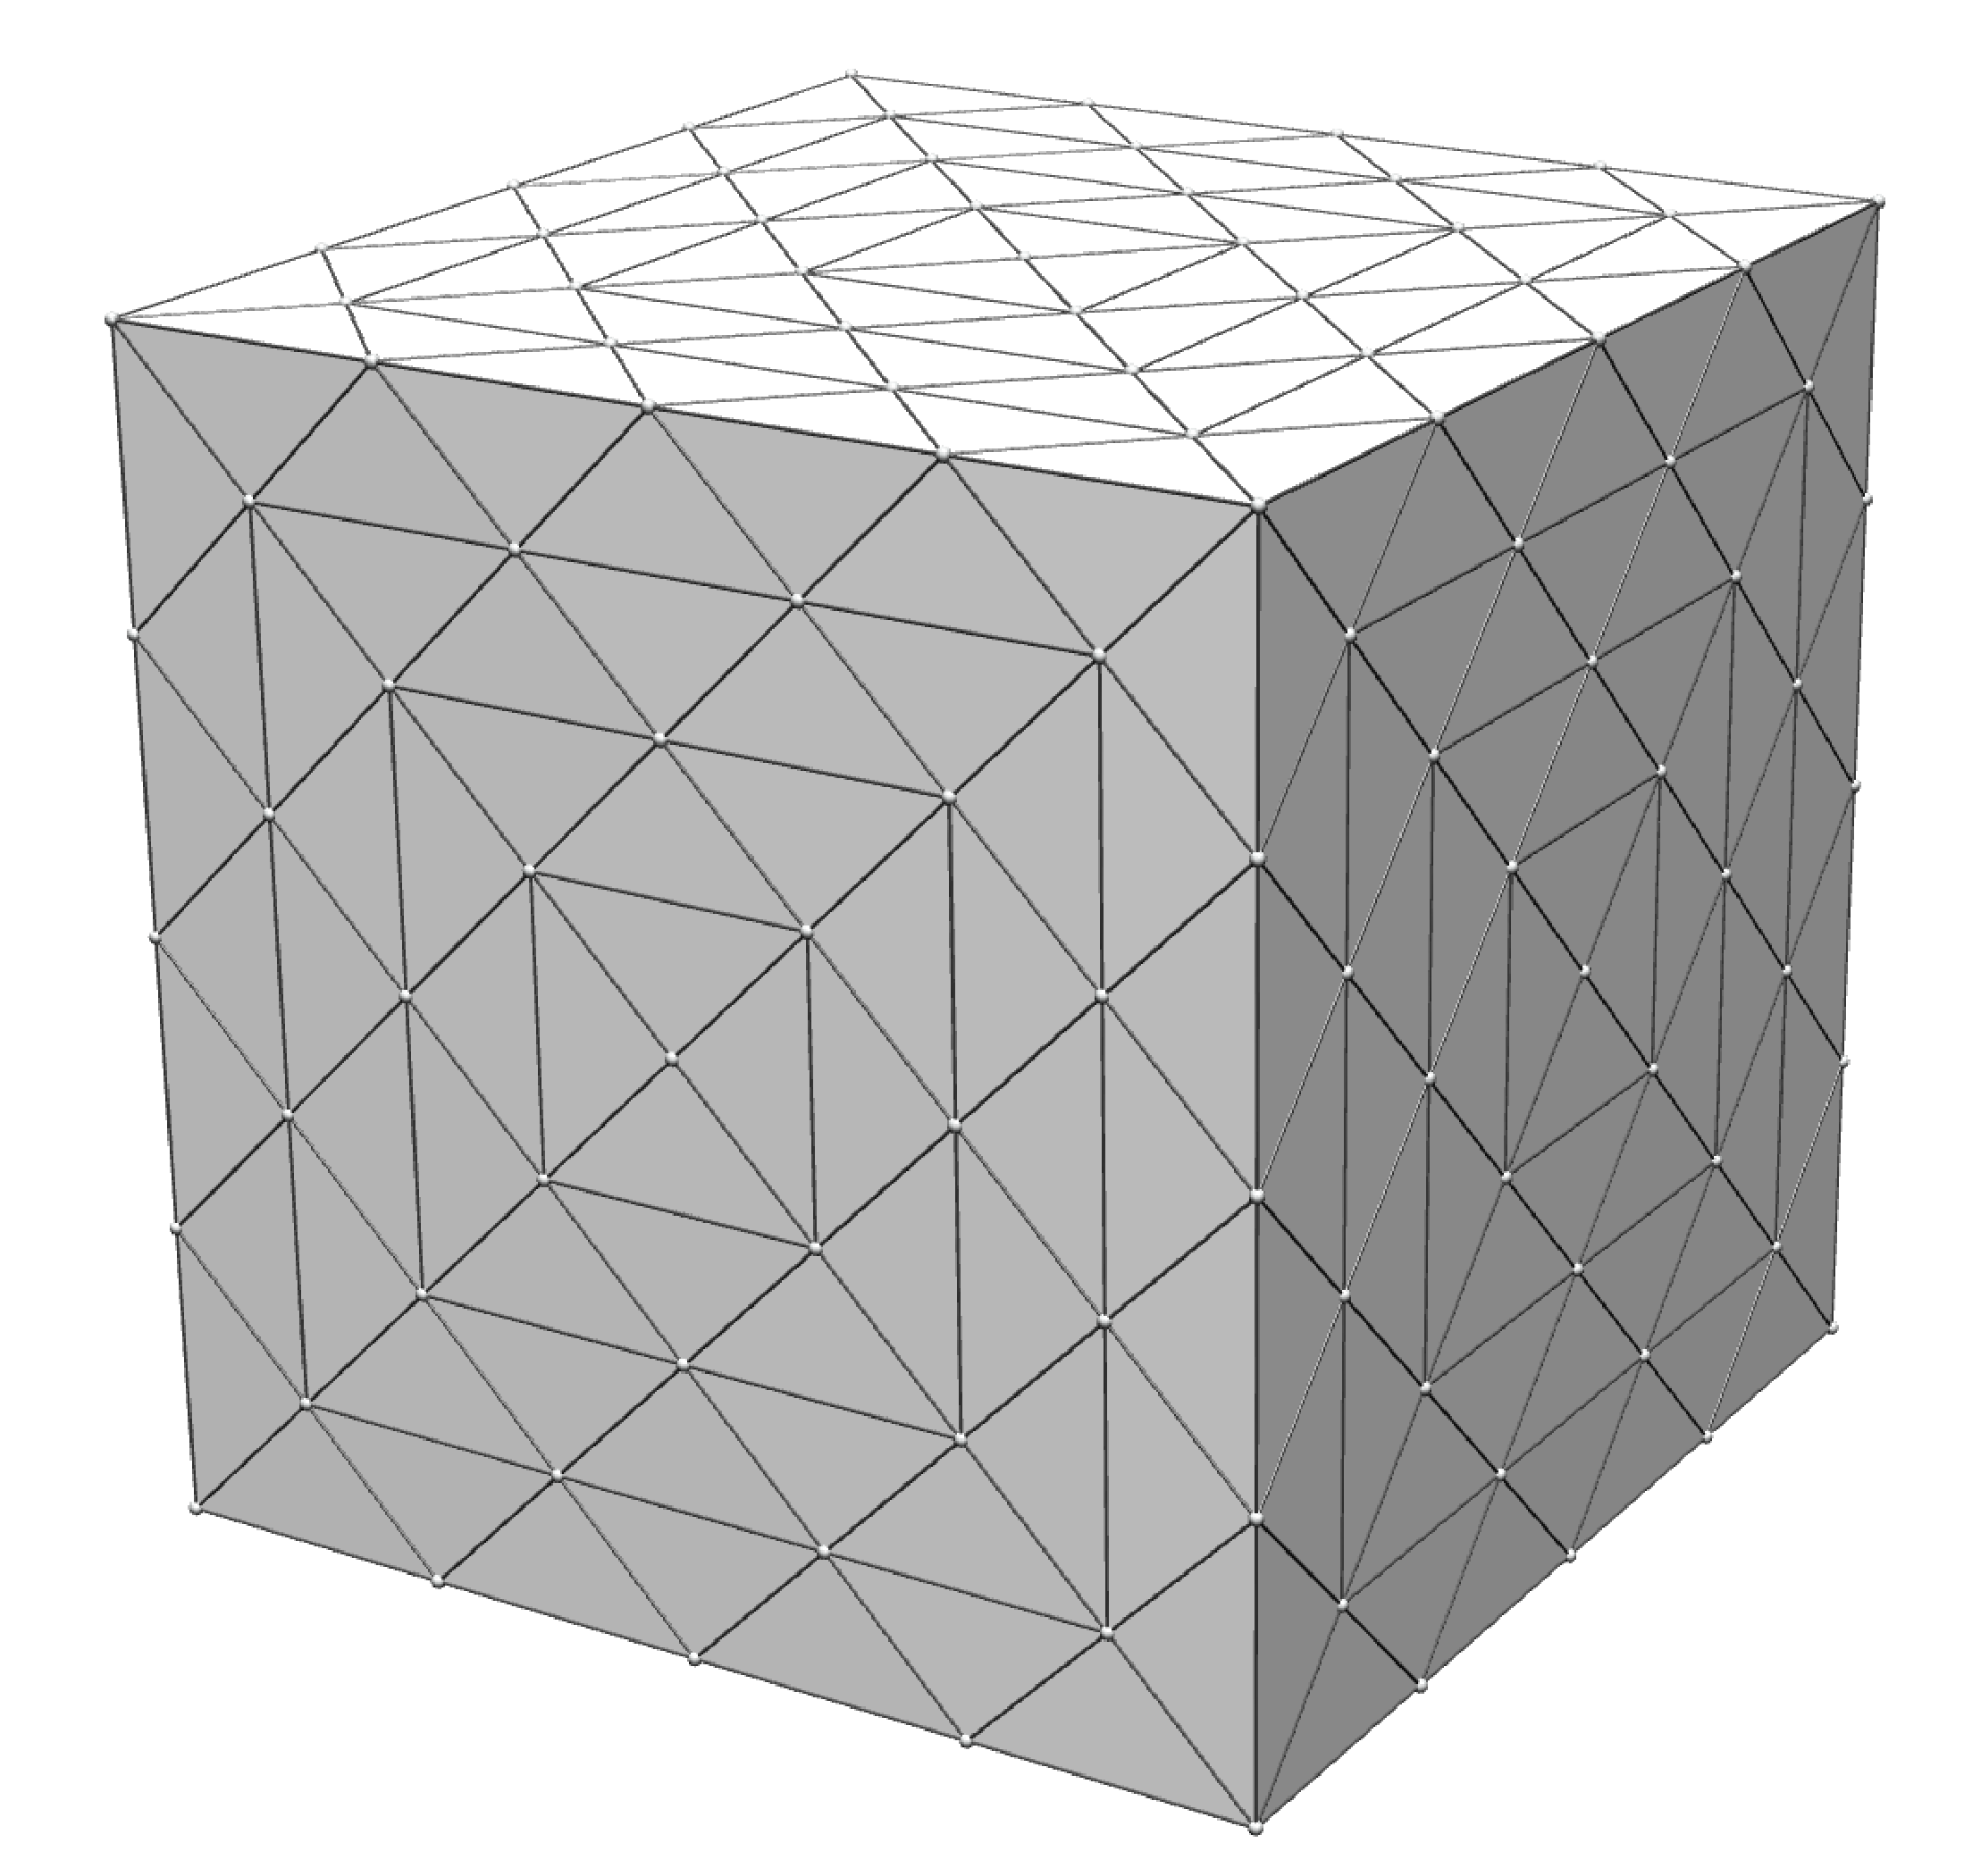
\includegraphics[height=5cm]{spherical/cube_image.pdf}
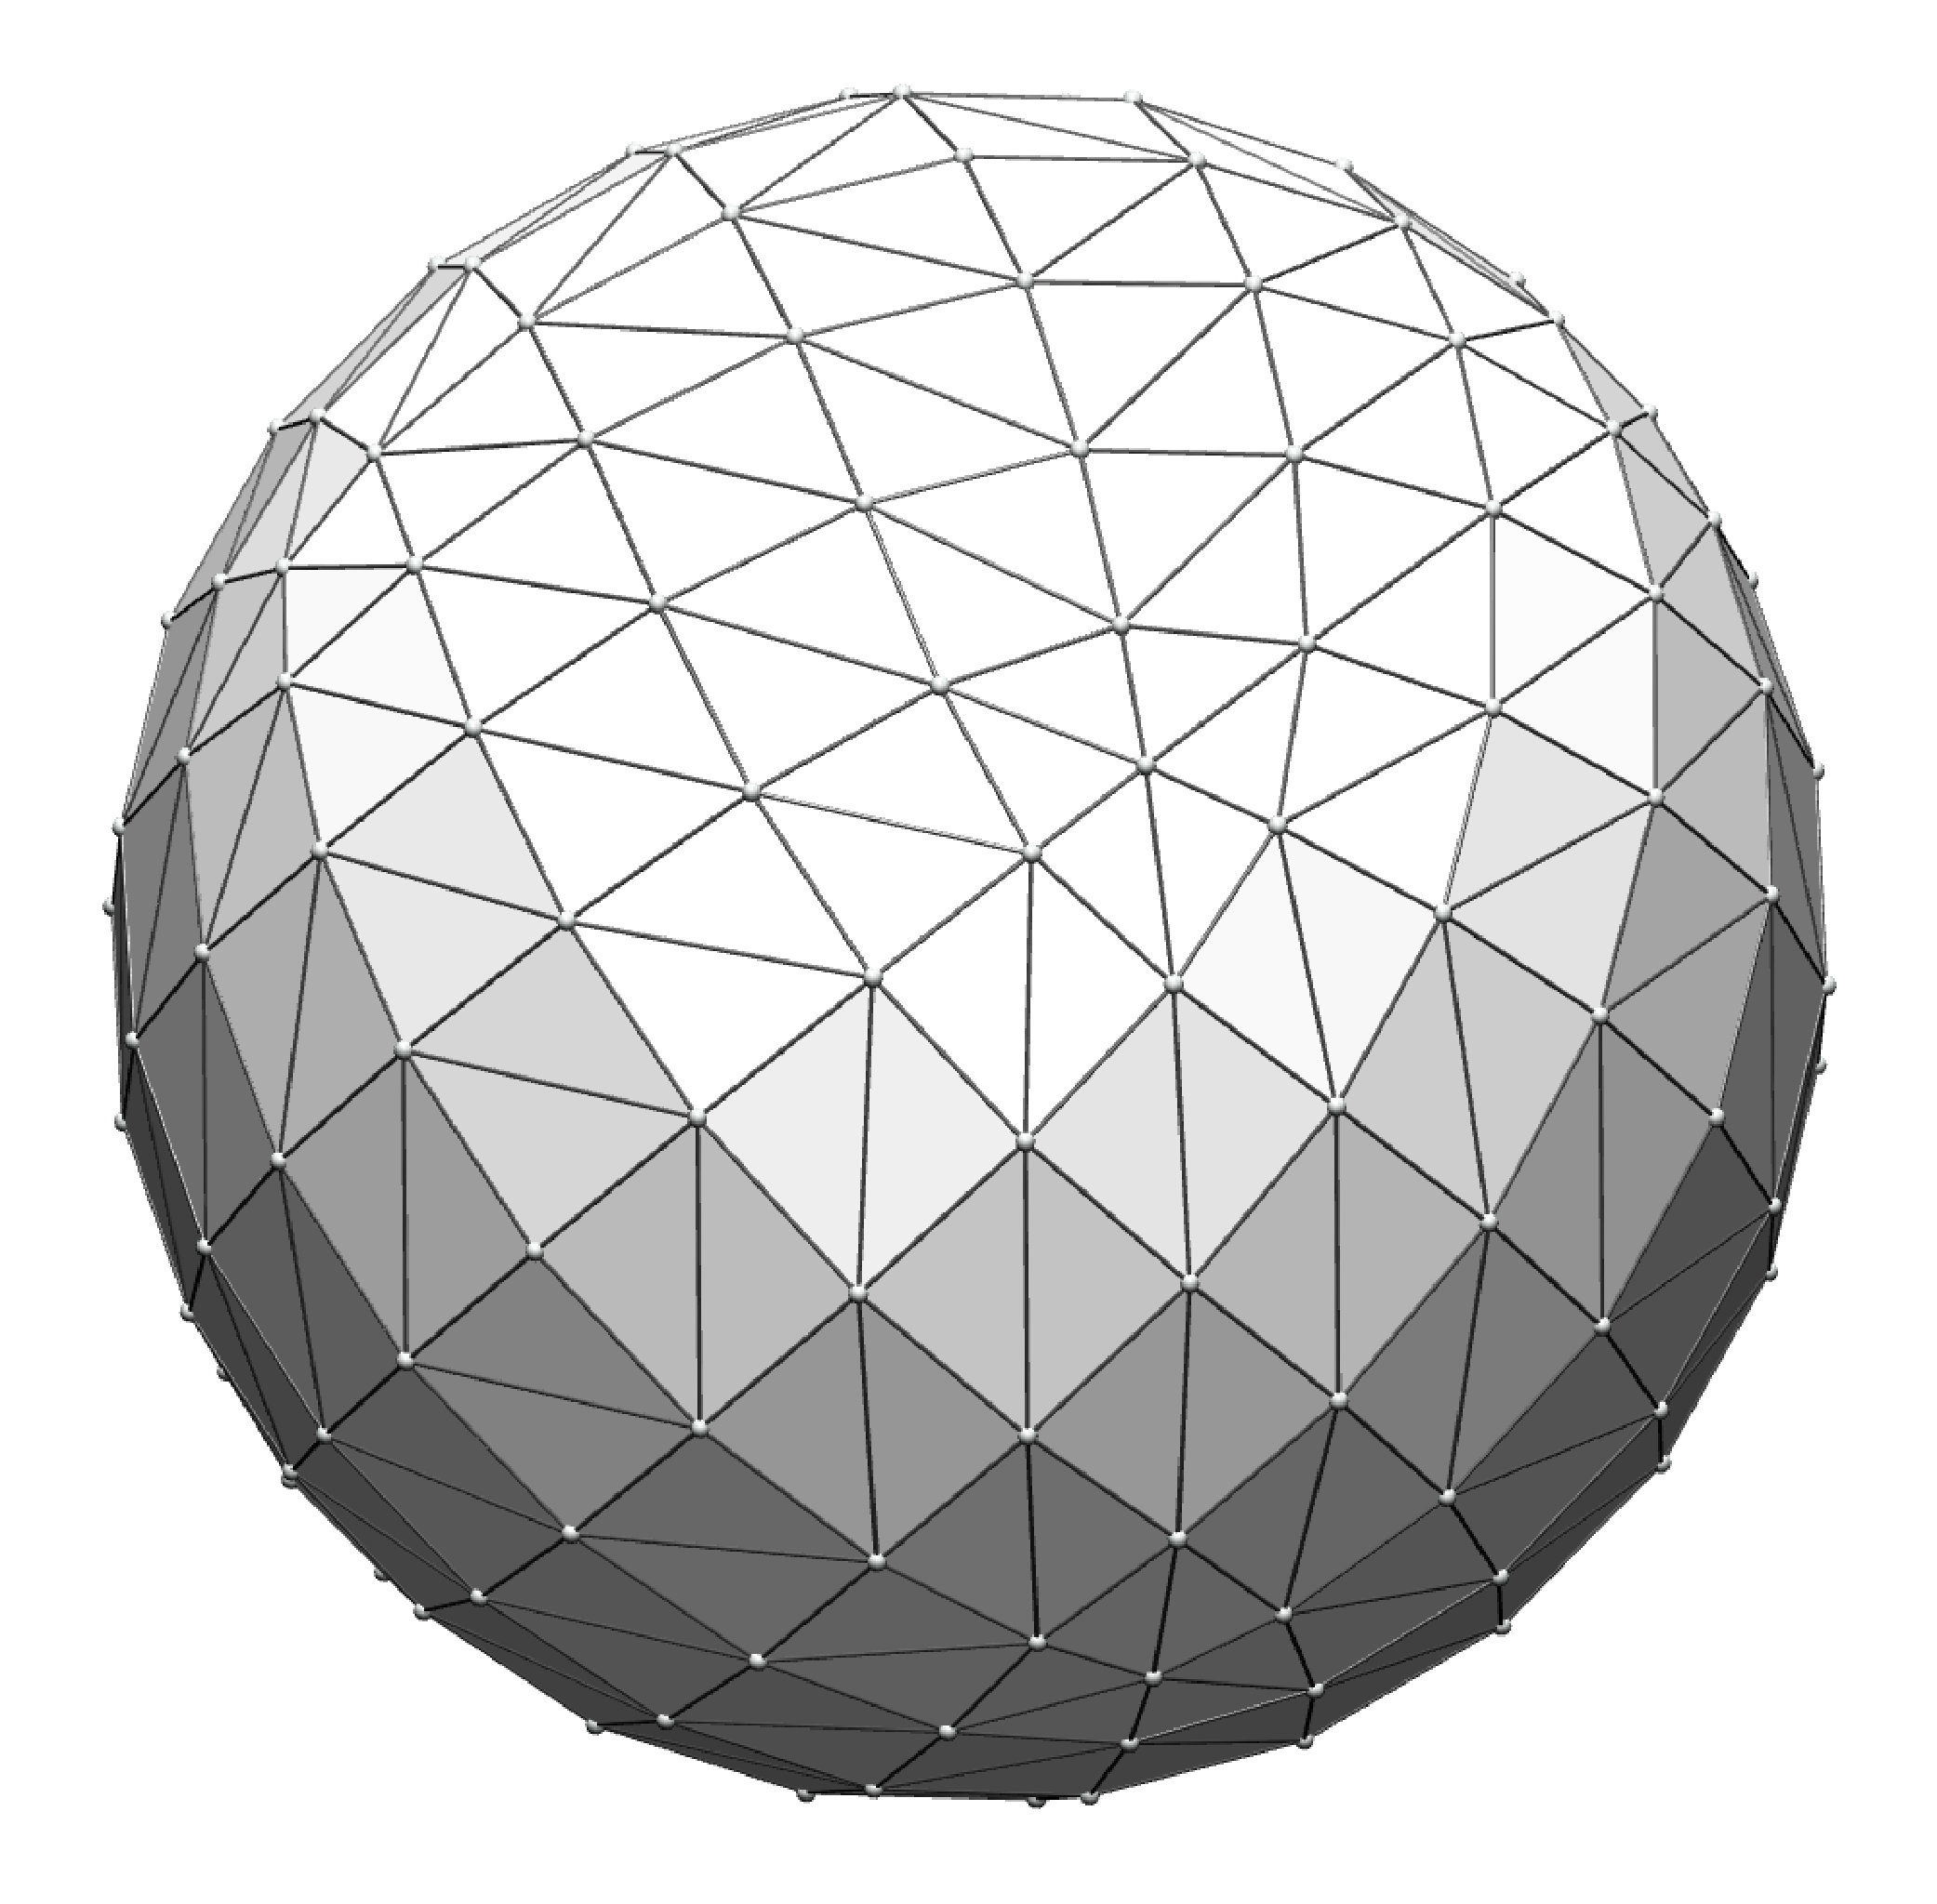
\includegraphics[height=5cm]{spherical/cube_domain.pdf}
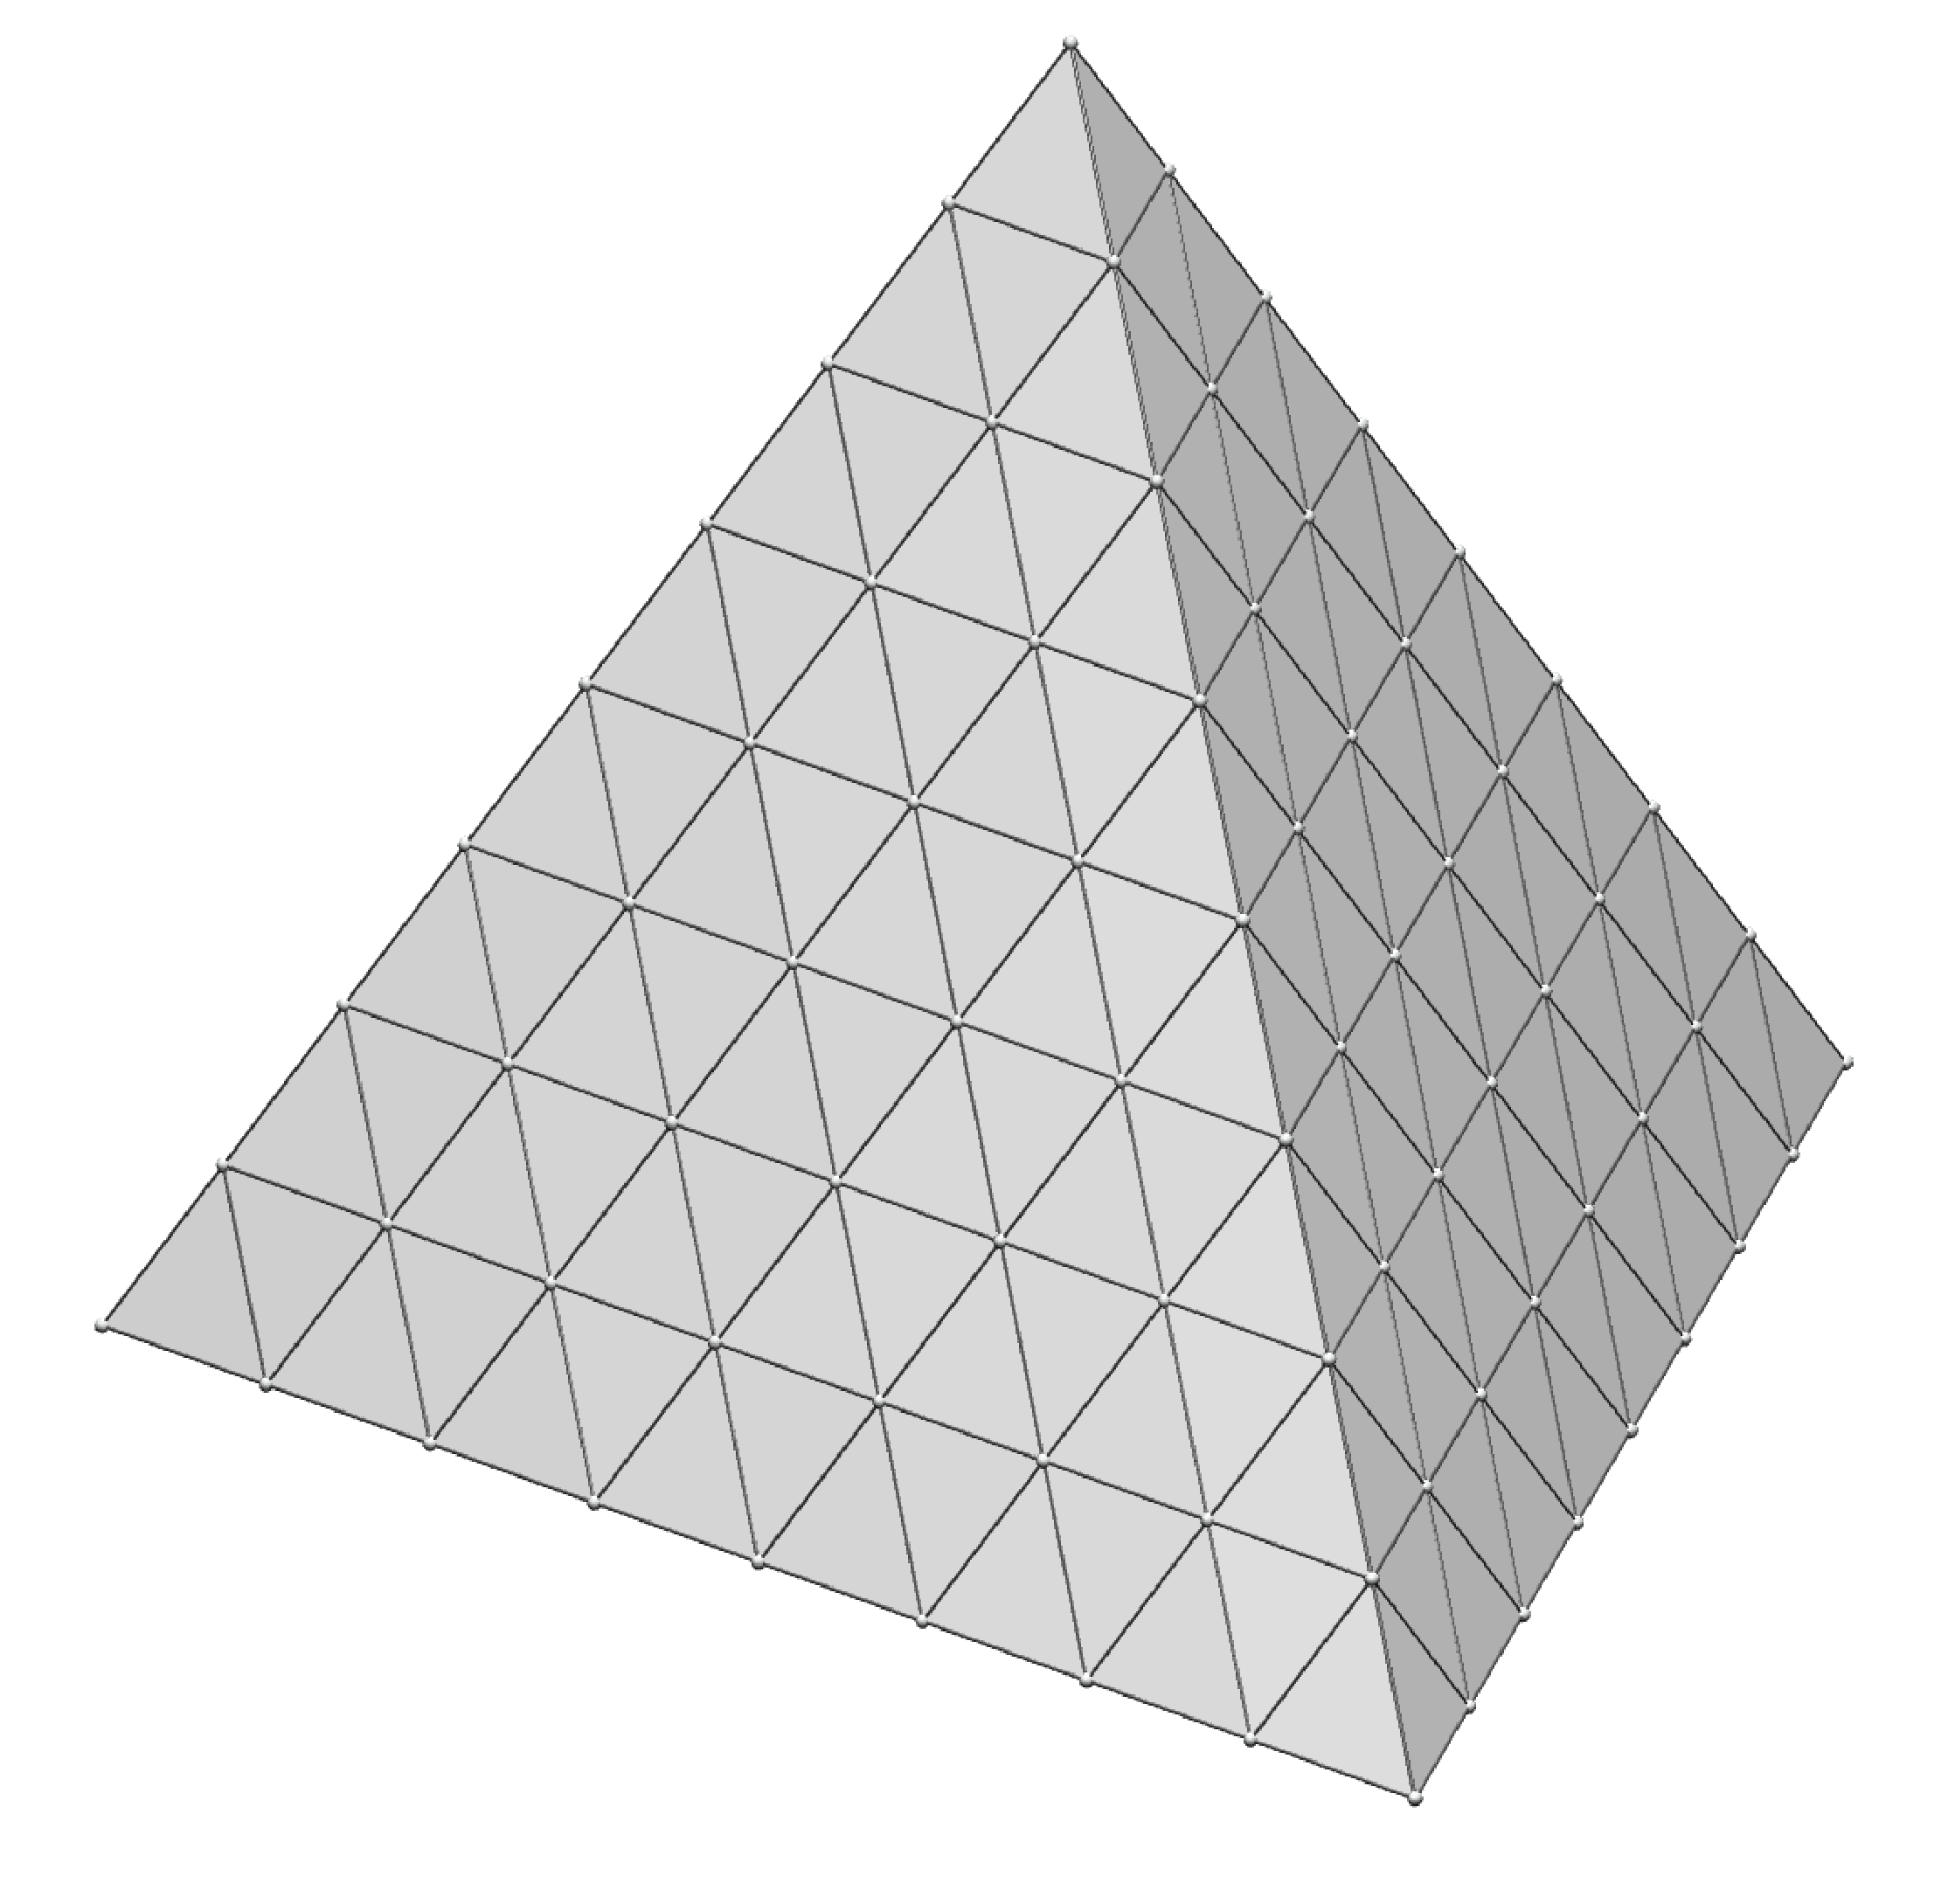
\includegraphics[height=5cm]{spherical/tetrahedron_image.pdf}
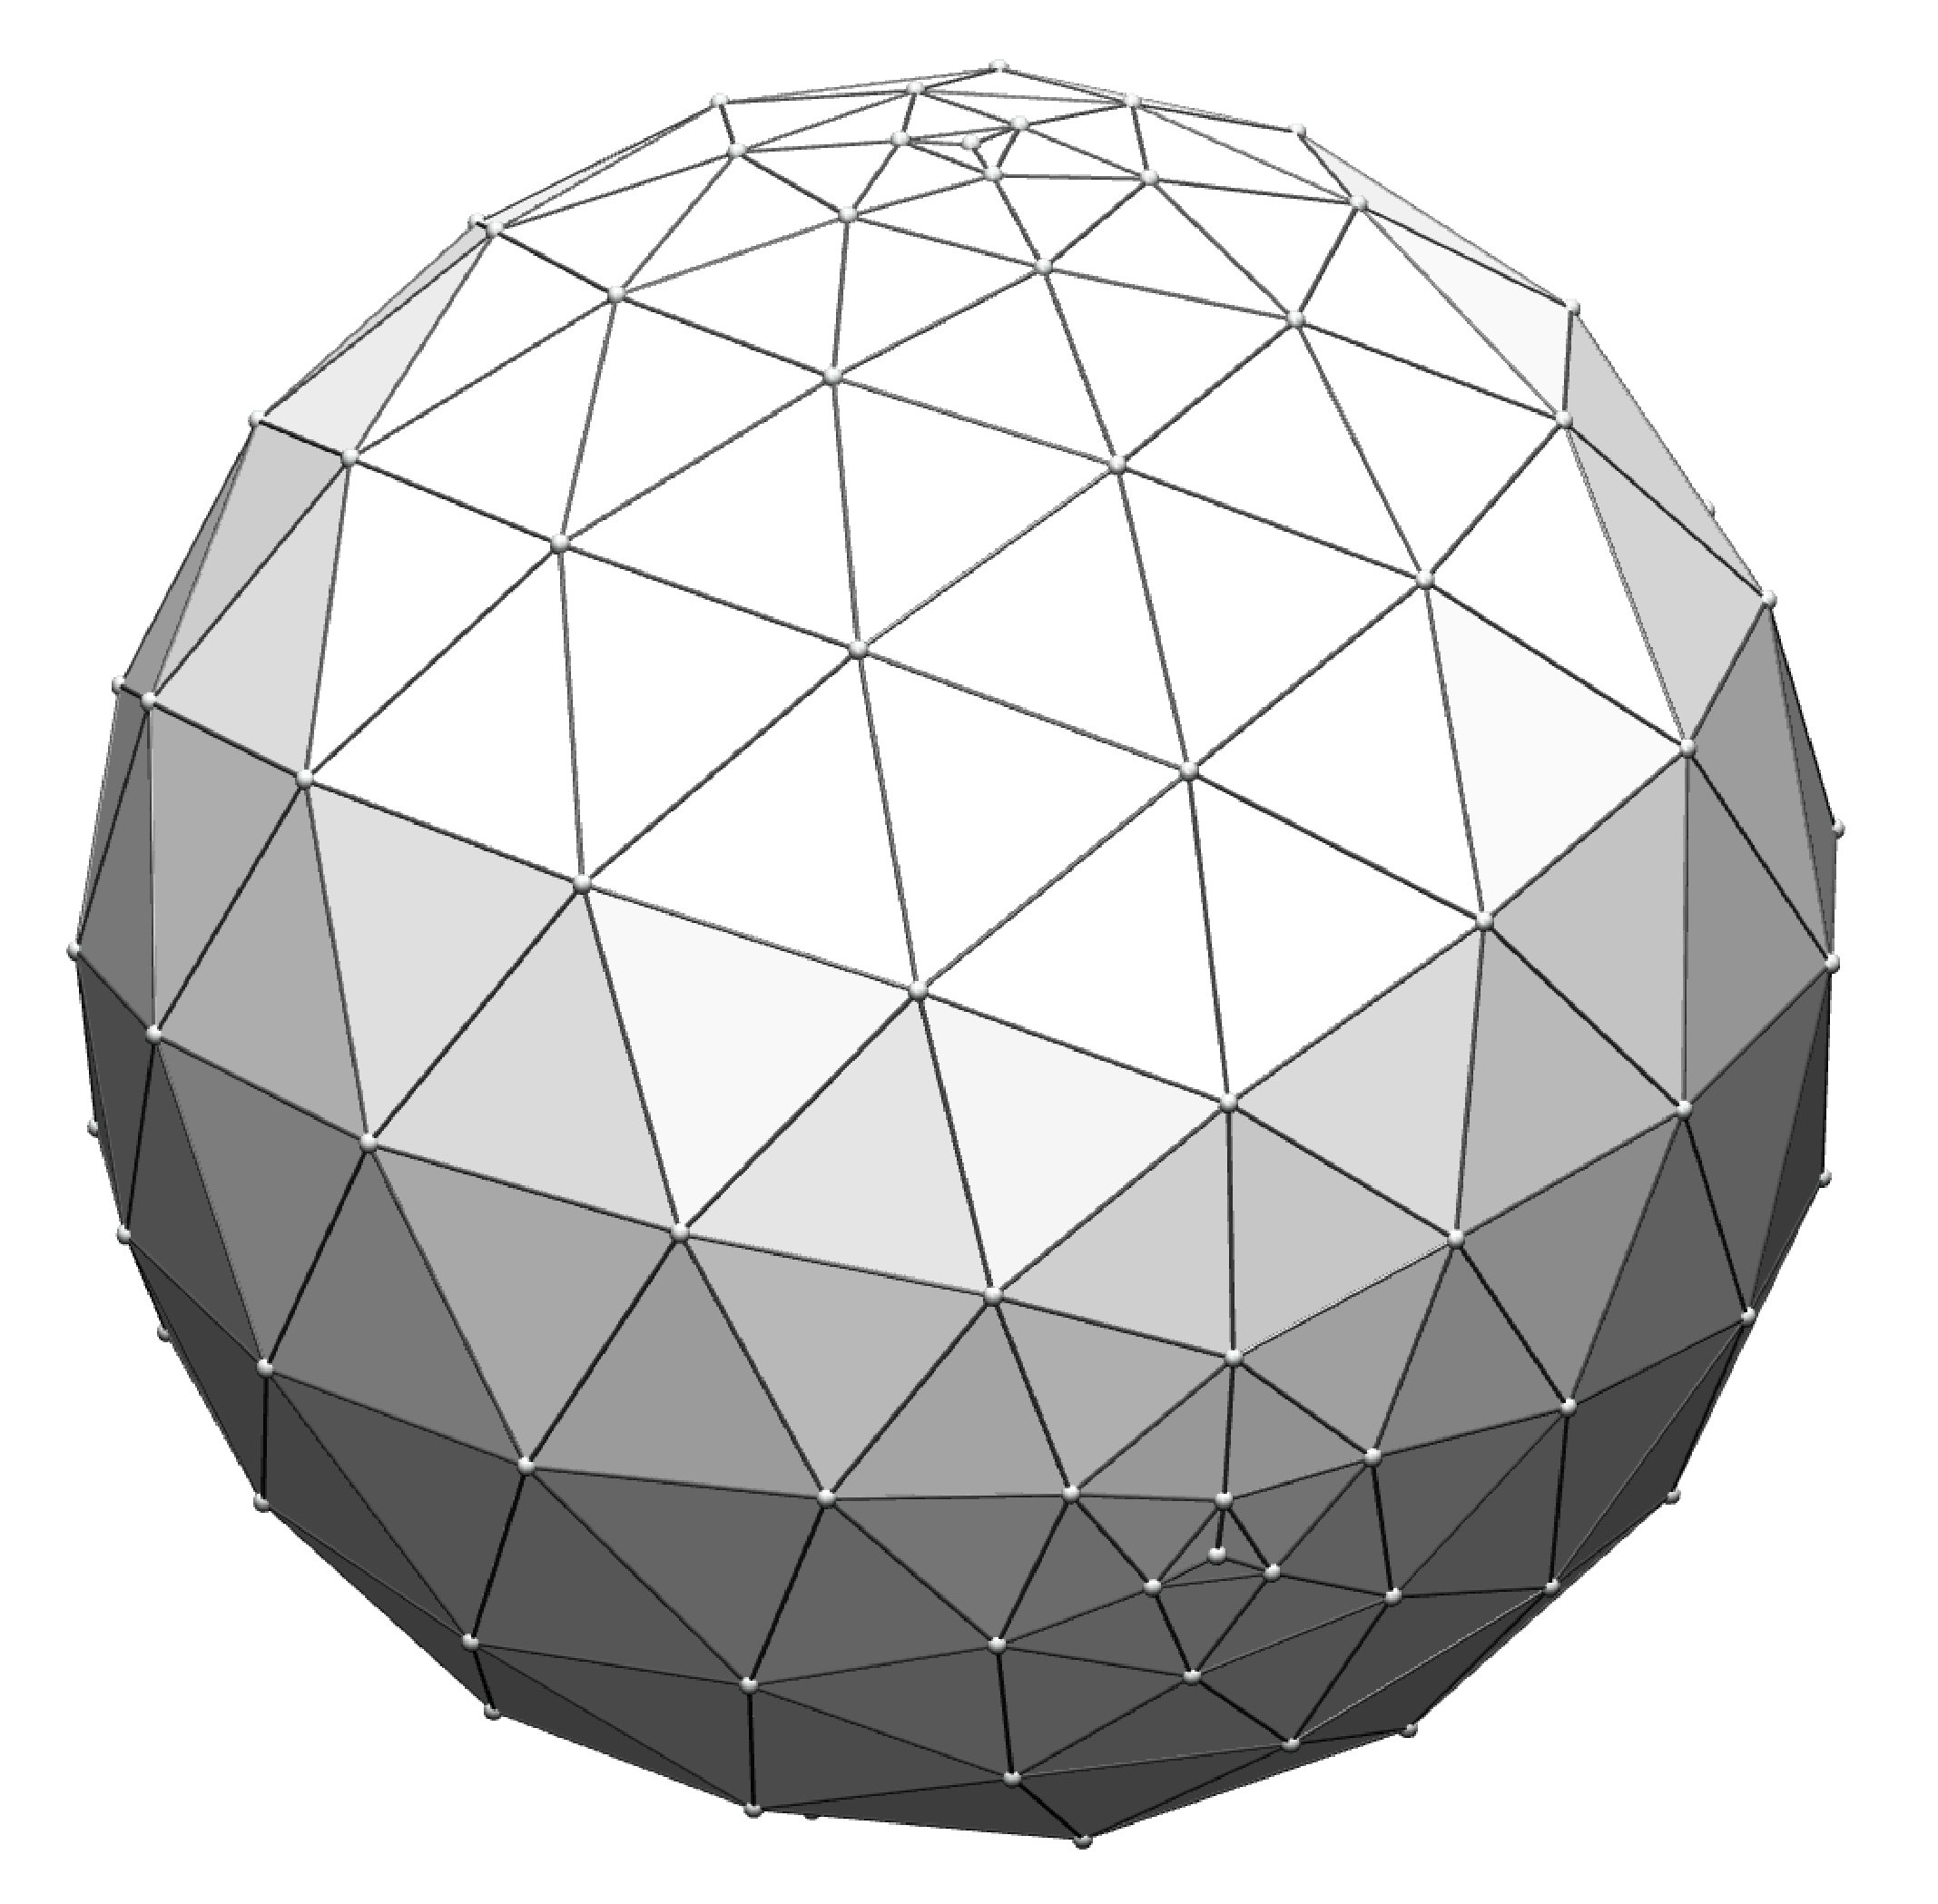
\includegraphics[height=5cm]{spherical/tetrahedron_domain.pdf}
}
\setstretch{0.0}{\scriptsize\tt data/spherical/cube\_data.xml}\quad\quad\quad\quad{\scriptsize\tt data/spherical/tetrahedron\_data.xml}
\caption{Mapping conformally to the sphere using the spherical functional and a direct spherical layout process. The image is normalized such that the center of mass of vertices is the center of the sphere.}
\label{fig:spherical_examples}
\end{figure}

It is possible to use the spherical functional to calculate spherical uniformizations even if it is non-convex. In this case a numerical optimization has to find a saddle point in the energy landscape. This is due to the fact that the direction $v=(1,\ldots,1)$ is a negative direction of the Hessian. That means shrinking or enlarging all scale factors at once decreases the value of the energy. We use a simple yet effective trick that enables us to find a critical point for certain examples. Define the reduced functional
\begin{equation}
\label{eq:reduced_spherical}
\tilde E^{\rm sph}(u)=\max_t \left\{E^{\rm sph}(u + tv)\right\}
\end{equation}
Now minimize the reduced functional $\tilde  E^{\rm sph}$. 
Following this scheme we create examples that would not be possible using simple minimization with arbitrary initialization, see Figure~\ref{fig:spherical_examples}.

\subsection{M{\"o}bius normalization}
\label{sec:moebius_normalization}
The description of conformal equivalence is M{\"o}bus invariant.  
To select a unique representative on the sphere we find the M{\"o}bius transformation $T$ such that
\[\sum_{i=1}^{n}T\cdot v_i = 0,\]
i.e., the center of mass of the points is the origin, see~\cite{Springborn05}.
To find the point of minimum hyperbolic distance sum as stated by Springborn we minimize the following functional. 
\begin{eqnarray*} 
	E(x) &=& \sum_{v\in V}\log\left(\frac{-\left<x,v\right>}{\sqrt{-\left<x,x\right>}}\right)\\
	\frac{\mathrm d E}{\mathrm dx} &=& \sum_{v\in V}\left(\frac{v}{\left<x,v\right>} - \frac{x}{\left<x,x\right>}\right)\\
	\frac{\mathrm d^2 E}{\mathrm dx^2} &=& \sum_{v\in V}\left(2\frac{x^Tx}{\left<x,x\right>^2}-\frac{v^Tv}{\left<x,v\right>^2} - \mathrm{diag}\left(\frac{1}{\left<x,x\right>}\right)\right)
\end{eqnarray*}
Here $\left<.,.\right>$ is the Minkowski scalar product. Note that the problem is
 $3$-dimensional and as such we define $\left<x,y\right>\vcentcolon=x_1y_1+x_2y_2+x_3y_3-1$ in
the implementation.

\subsection{Euclidean uniformization of spheres}

\begin{figure}
\centering
\resizebox{\textwidth}{!}{
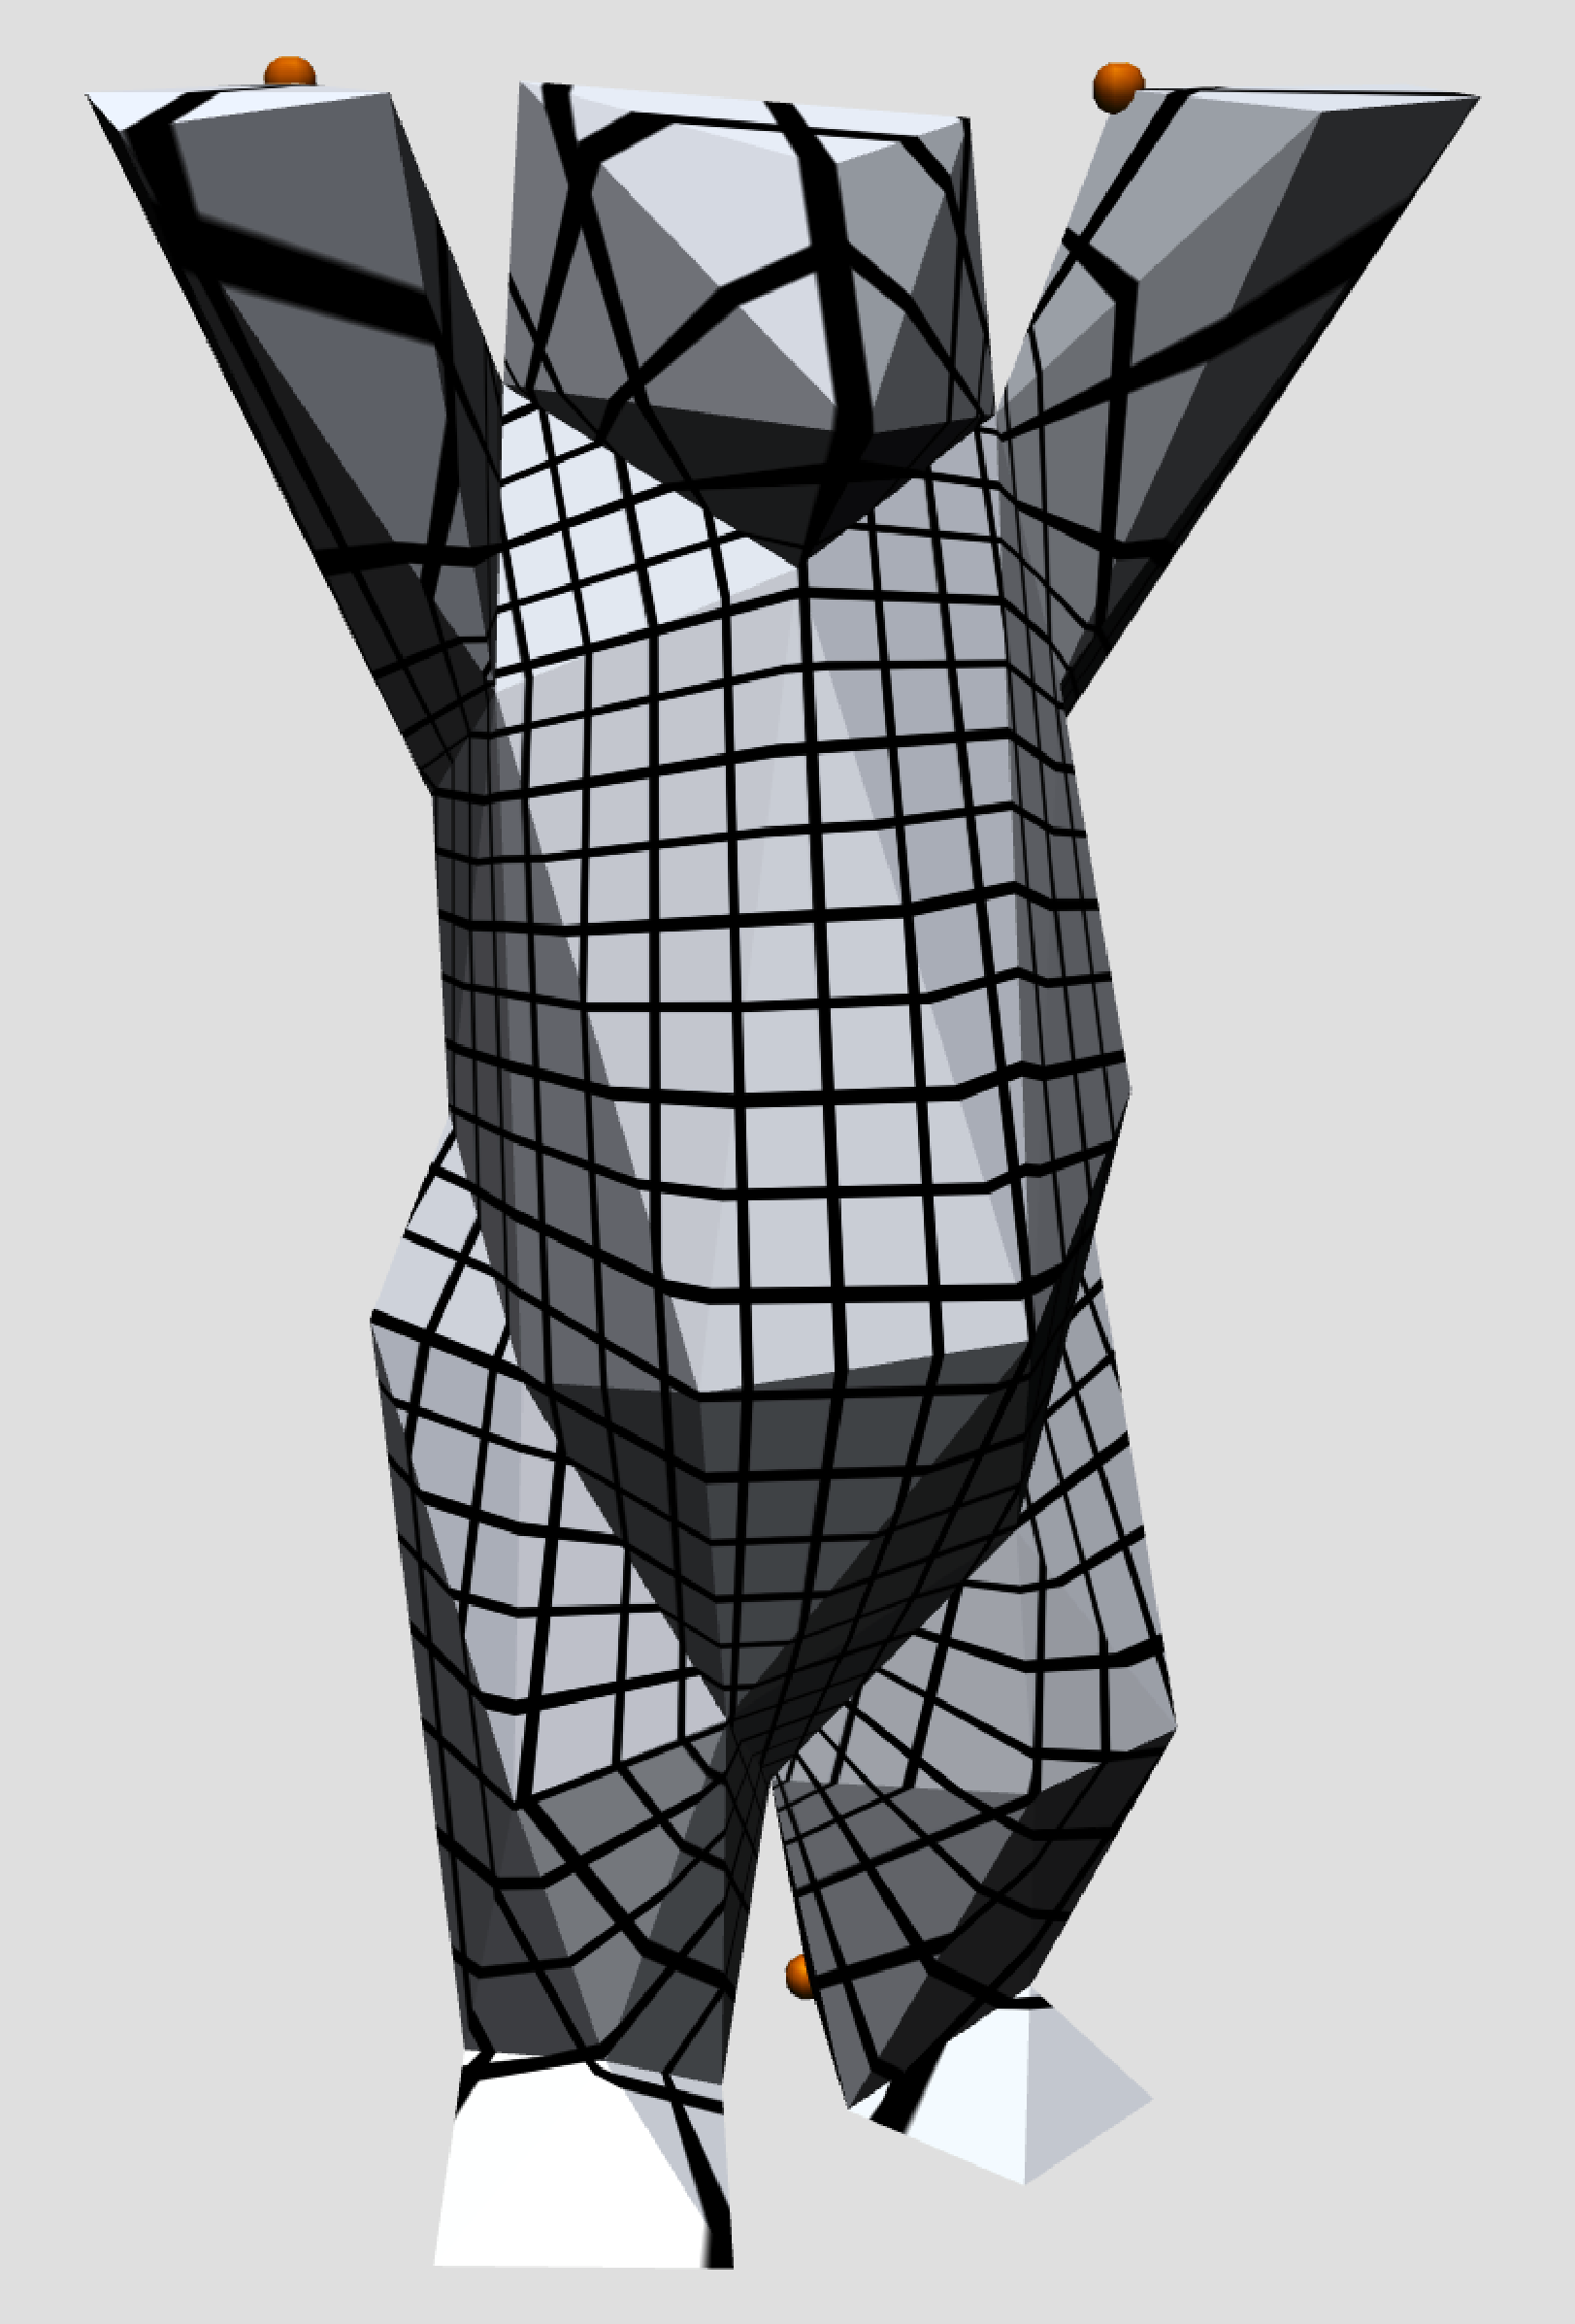
\includegraphics[height=10cm]{bear_torus/baer_quads.pdf}
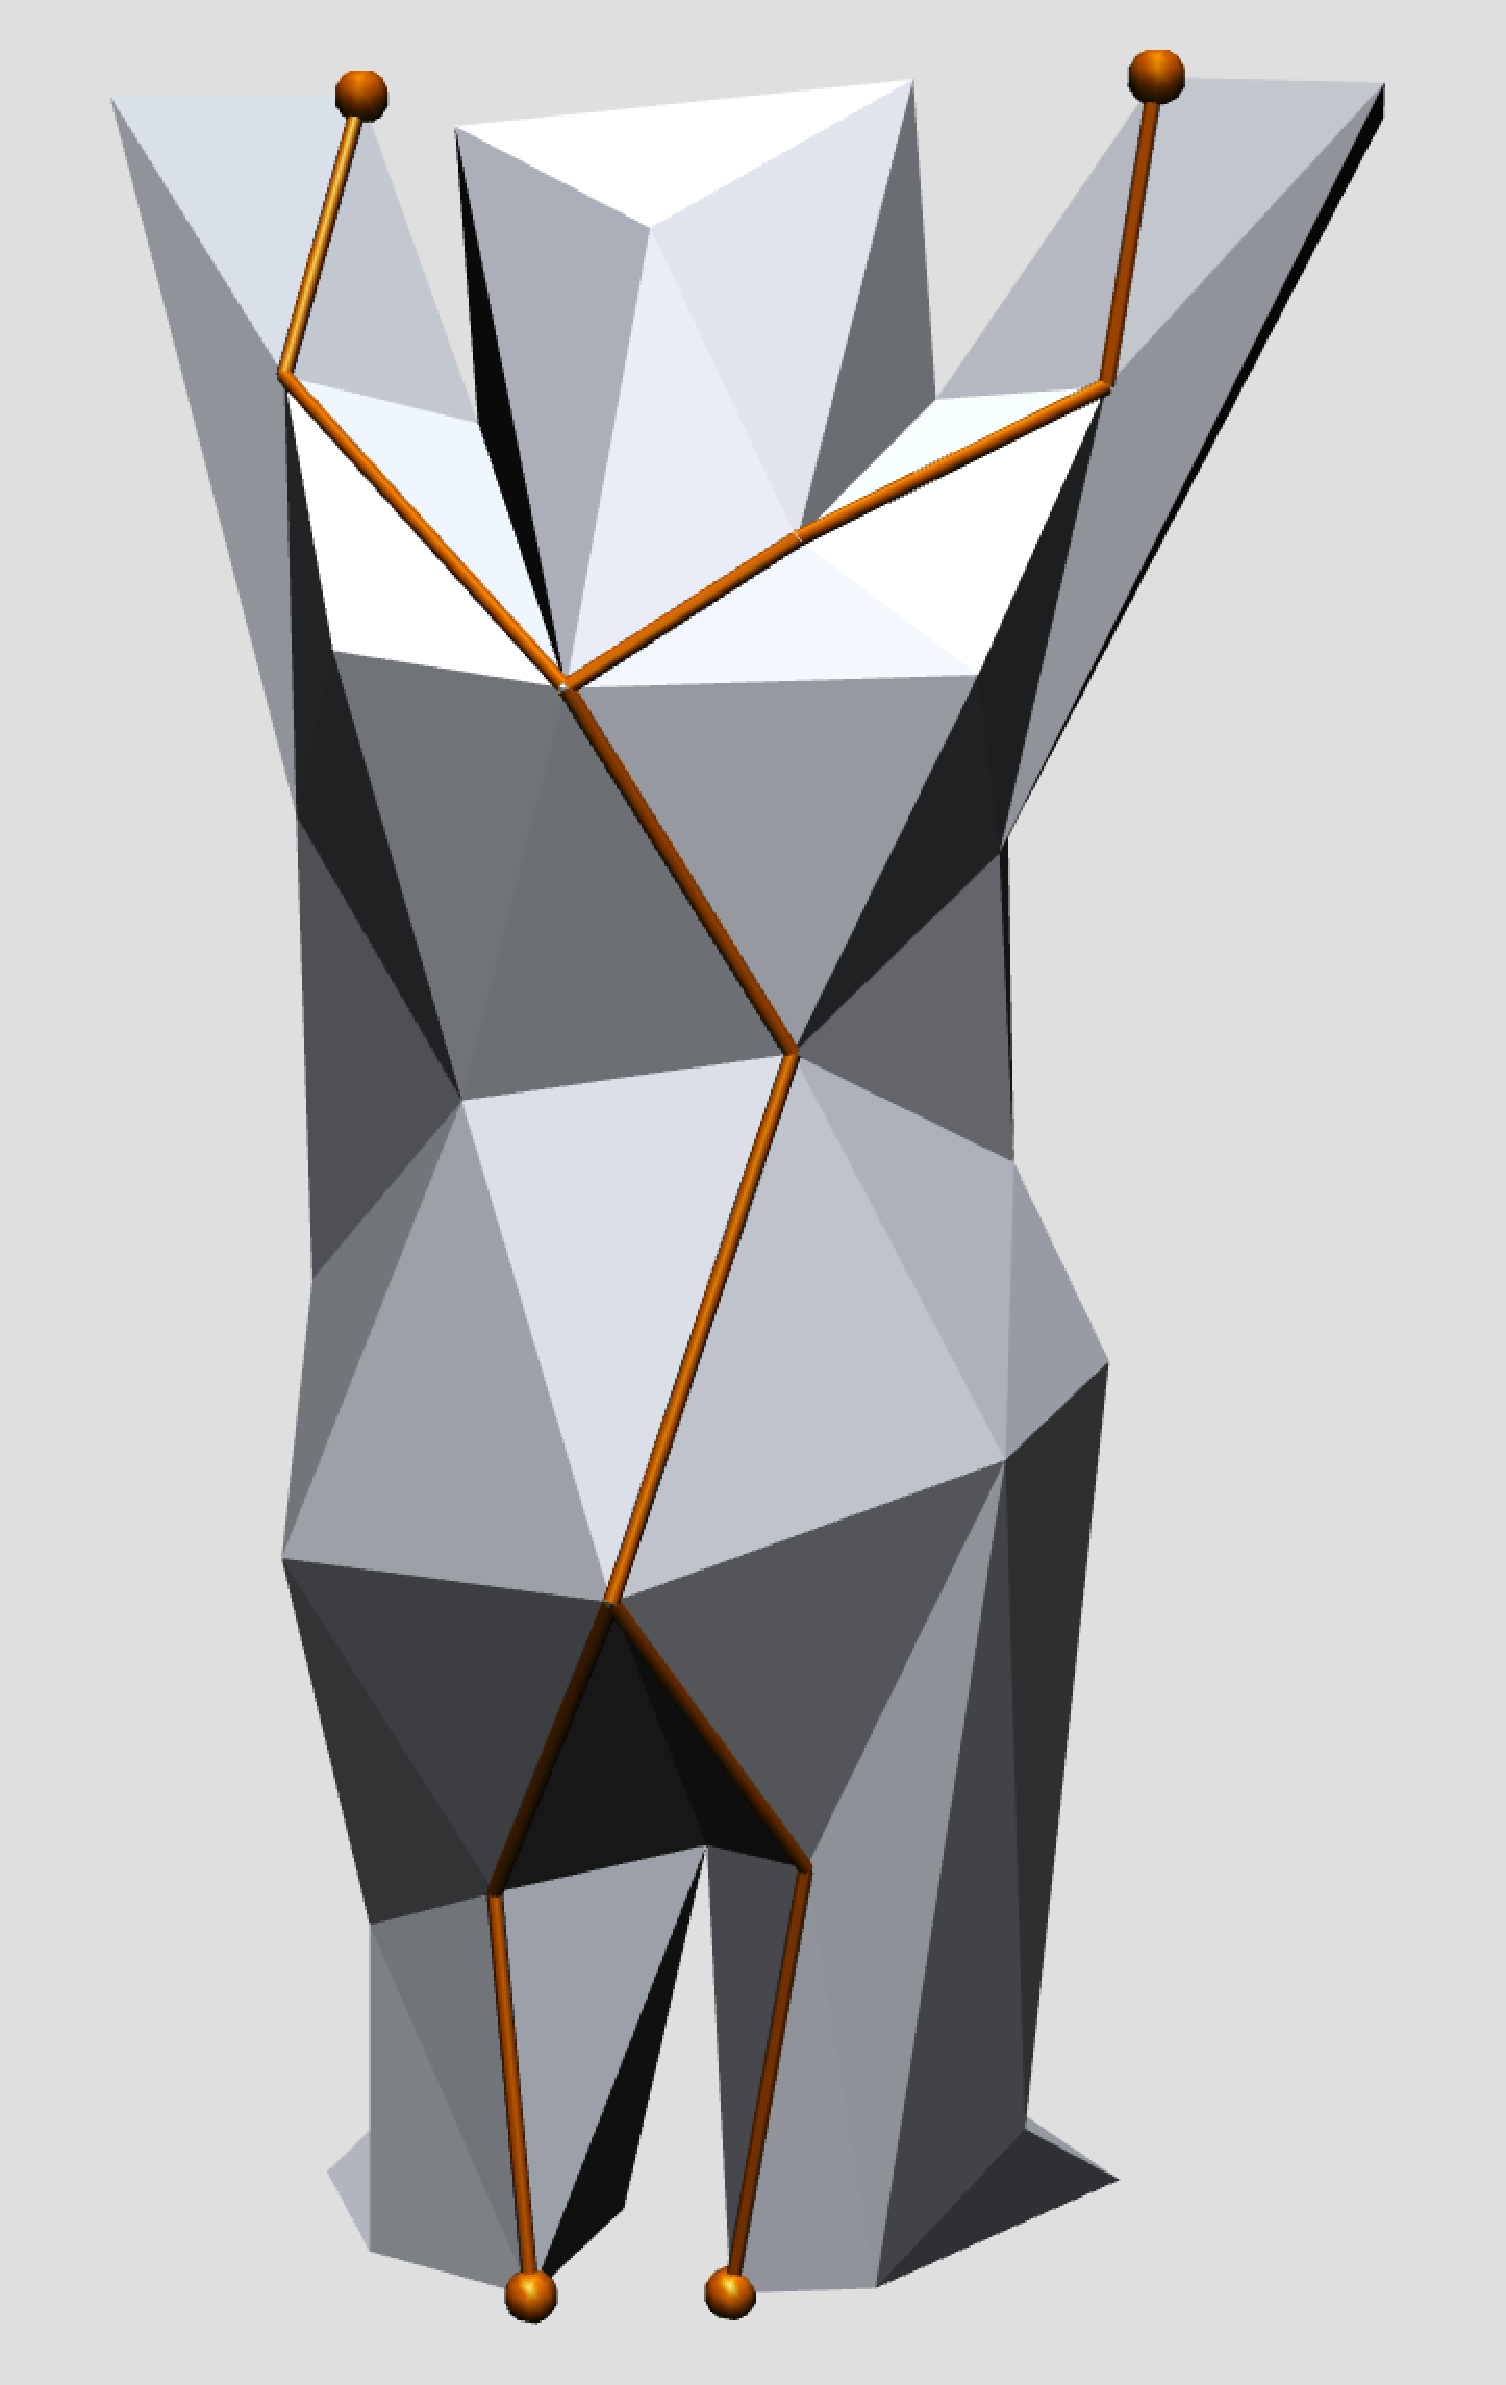
\includegraphics[height=10cm]{bear_torus/baer_cuts.pdf}
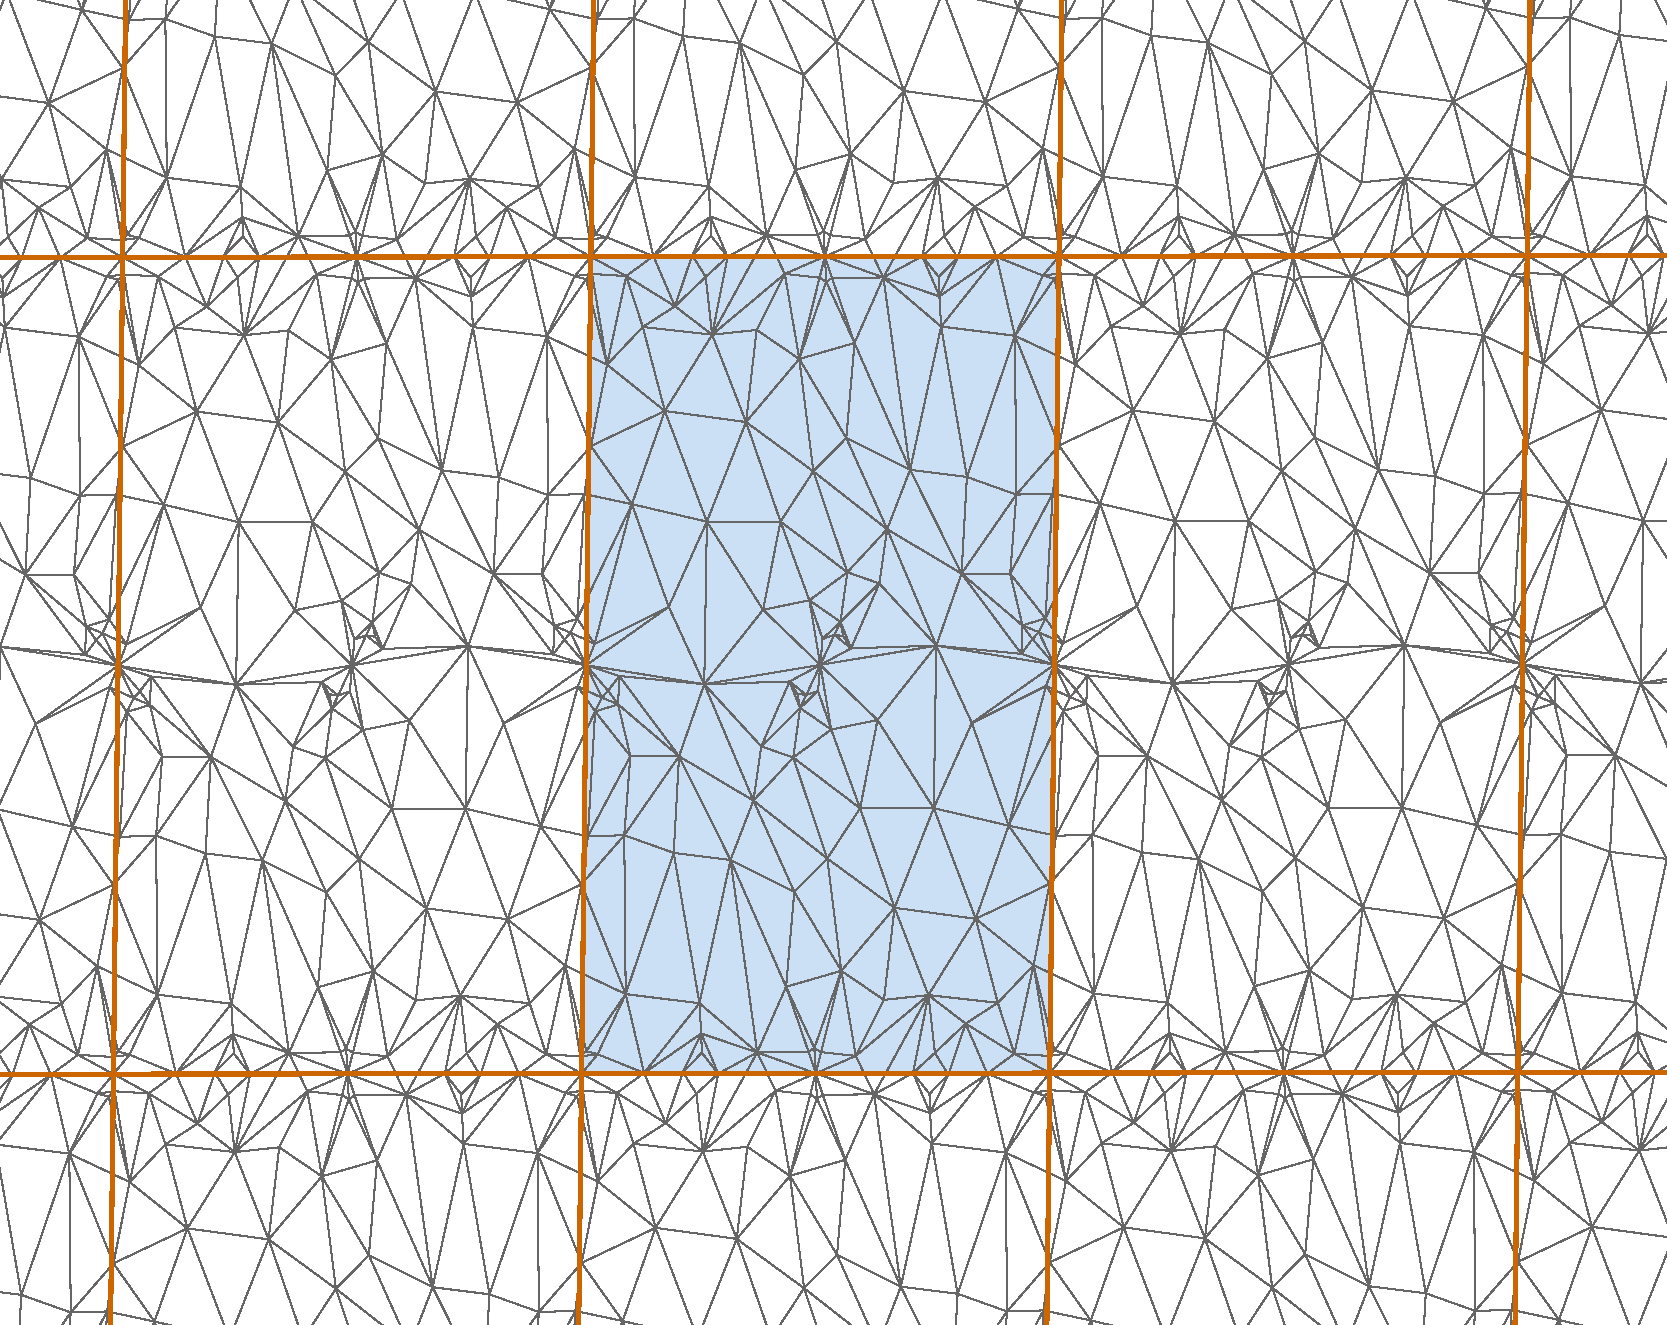
\includegraphics[height=10cm]{bear_torus/cover_triangulation_rectangle.pdf}
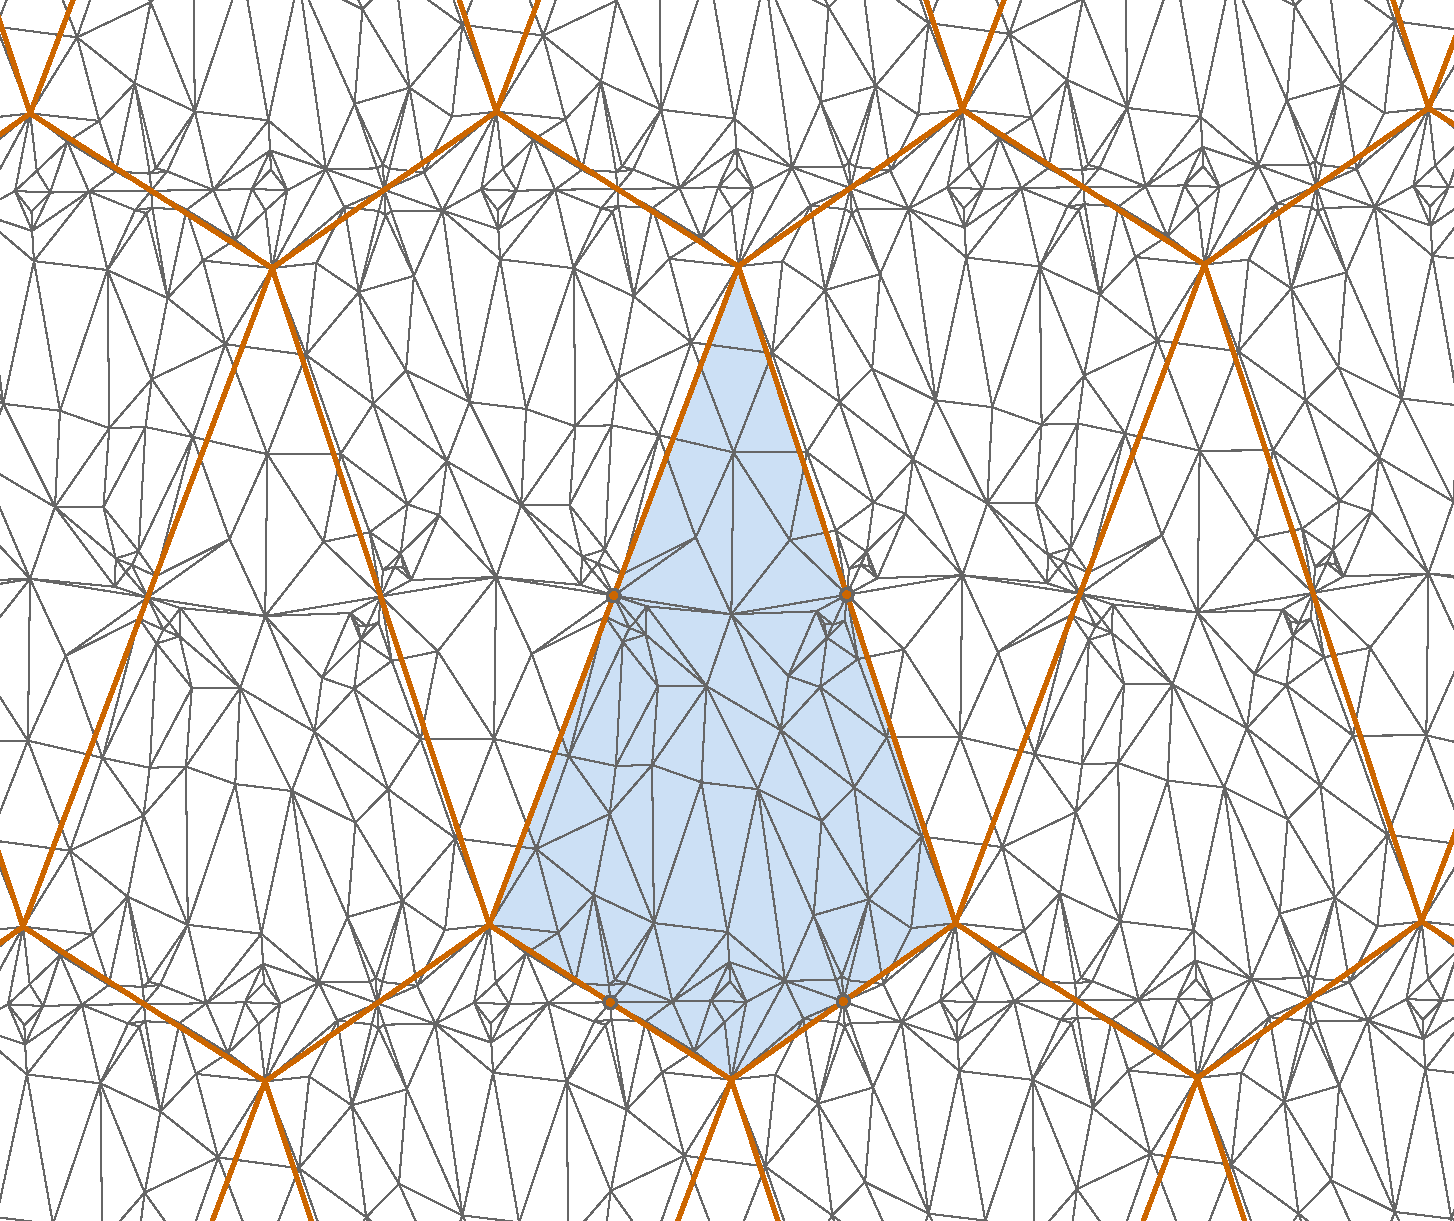
\includegraphics[height=10cm]{bear_torus/cover_triangulation.pdf}
}\\
\setstretch{0.8}{\scriptsize\tt data/bear\_torus/bear60.xml}
\caption{
A discrete bear model is mapped to the plane.
Four cone-like singularities of angle $\pi$ are chosen at the arms and legs to reduce the conformal distortion.
The singularities can be interpreted as branch points of a two-sheeted cover of the bear forming a topological torus.
The corresponding universal cover is generated by euclidean translations, the fundamental domain can be chosen to be an approximate rectangle, middle.
The group of translations is a subgroup of the group generated by the rotations around the singularities about and angle of $\pi$. In a fundamental domain the branch vertices lie in the middle of edges, right.
}
\label{fig:bear}
\end{figure}

A branched cover of a topological sphere with four branch points is a topological torus.
We exploit this fact to calculate parameterizations of triangulations with spherical topology.
There are two ways to realize this.

We pick four vertices of the spherical triangulation. We create a two-sheeted branched cover of the triangulation by glueing two copies along paths connecting the selected vertices.
This procedure is parallel to the creation of discrete elliptic curves described in Section~\ref{sec:discrete_algebraic_curves}.
The resulting surface is a topological torus and can be uniformized using the euclidean functional and a layout in the plane.
The uniformizing group is generated by two translations.
This group is a subgroup of the group generated by rotations around the branch vertices.
Hence we can as well prescribe cone angles of $\pi$ at the selected vertices and calculate a direct map to the plane.
The universal cover is then generated by rotations.

We apply this procedure to a model of a bear, see Figure~\ref{fig:bear}. To create the triangle layout we cut the model open along an edge tree including the branch vertices, see the second picture in the Figure.

\section{Uniformization of tori}
\label{sec:tori}

Every torus is conformally equivalent to a flat torus.
The conformal classes of flat tori can be parameterized by parallelogram lattices. 
Two lattices are equivalent if their complex edge ratios $\tau = \frac{\omega_1}{\omega_2}$ agree.
In this section we describe how to use discrete conformal maps to find analog constructions for discrete cyclic tori, see, e.g., Figure~\ref{fig:intro_uniformization}, middle. 
We show how to find conformally equivalent flat tori and their corresponding lattices for given polyhedral cyclic tori.

Section~\ref{sec:tori_schottky} introduces the discrete uniformization of tori given by Schottky data, i.e., a group of loxodromic transformations together with a set of circles in $\Chat$. 
In Section~\ref{sec:discrete_algebraic_curves} we treat tori given as algebraic curves, i.e., elliptic curves. 
We use elliptic curves to gain insight into the convergence behavior of discrete conformal maps in Section~\ref{sec:numerical_convergence}.

\begin{figure}
\centering
\resizebox{0.9\textwidth}{!}{
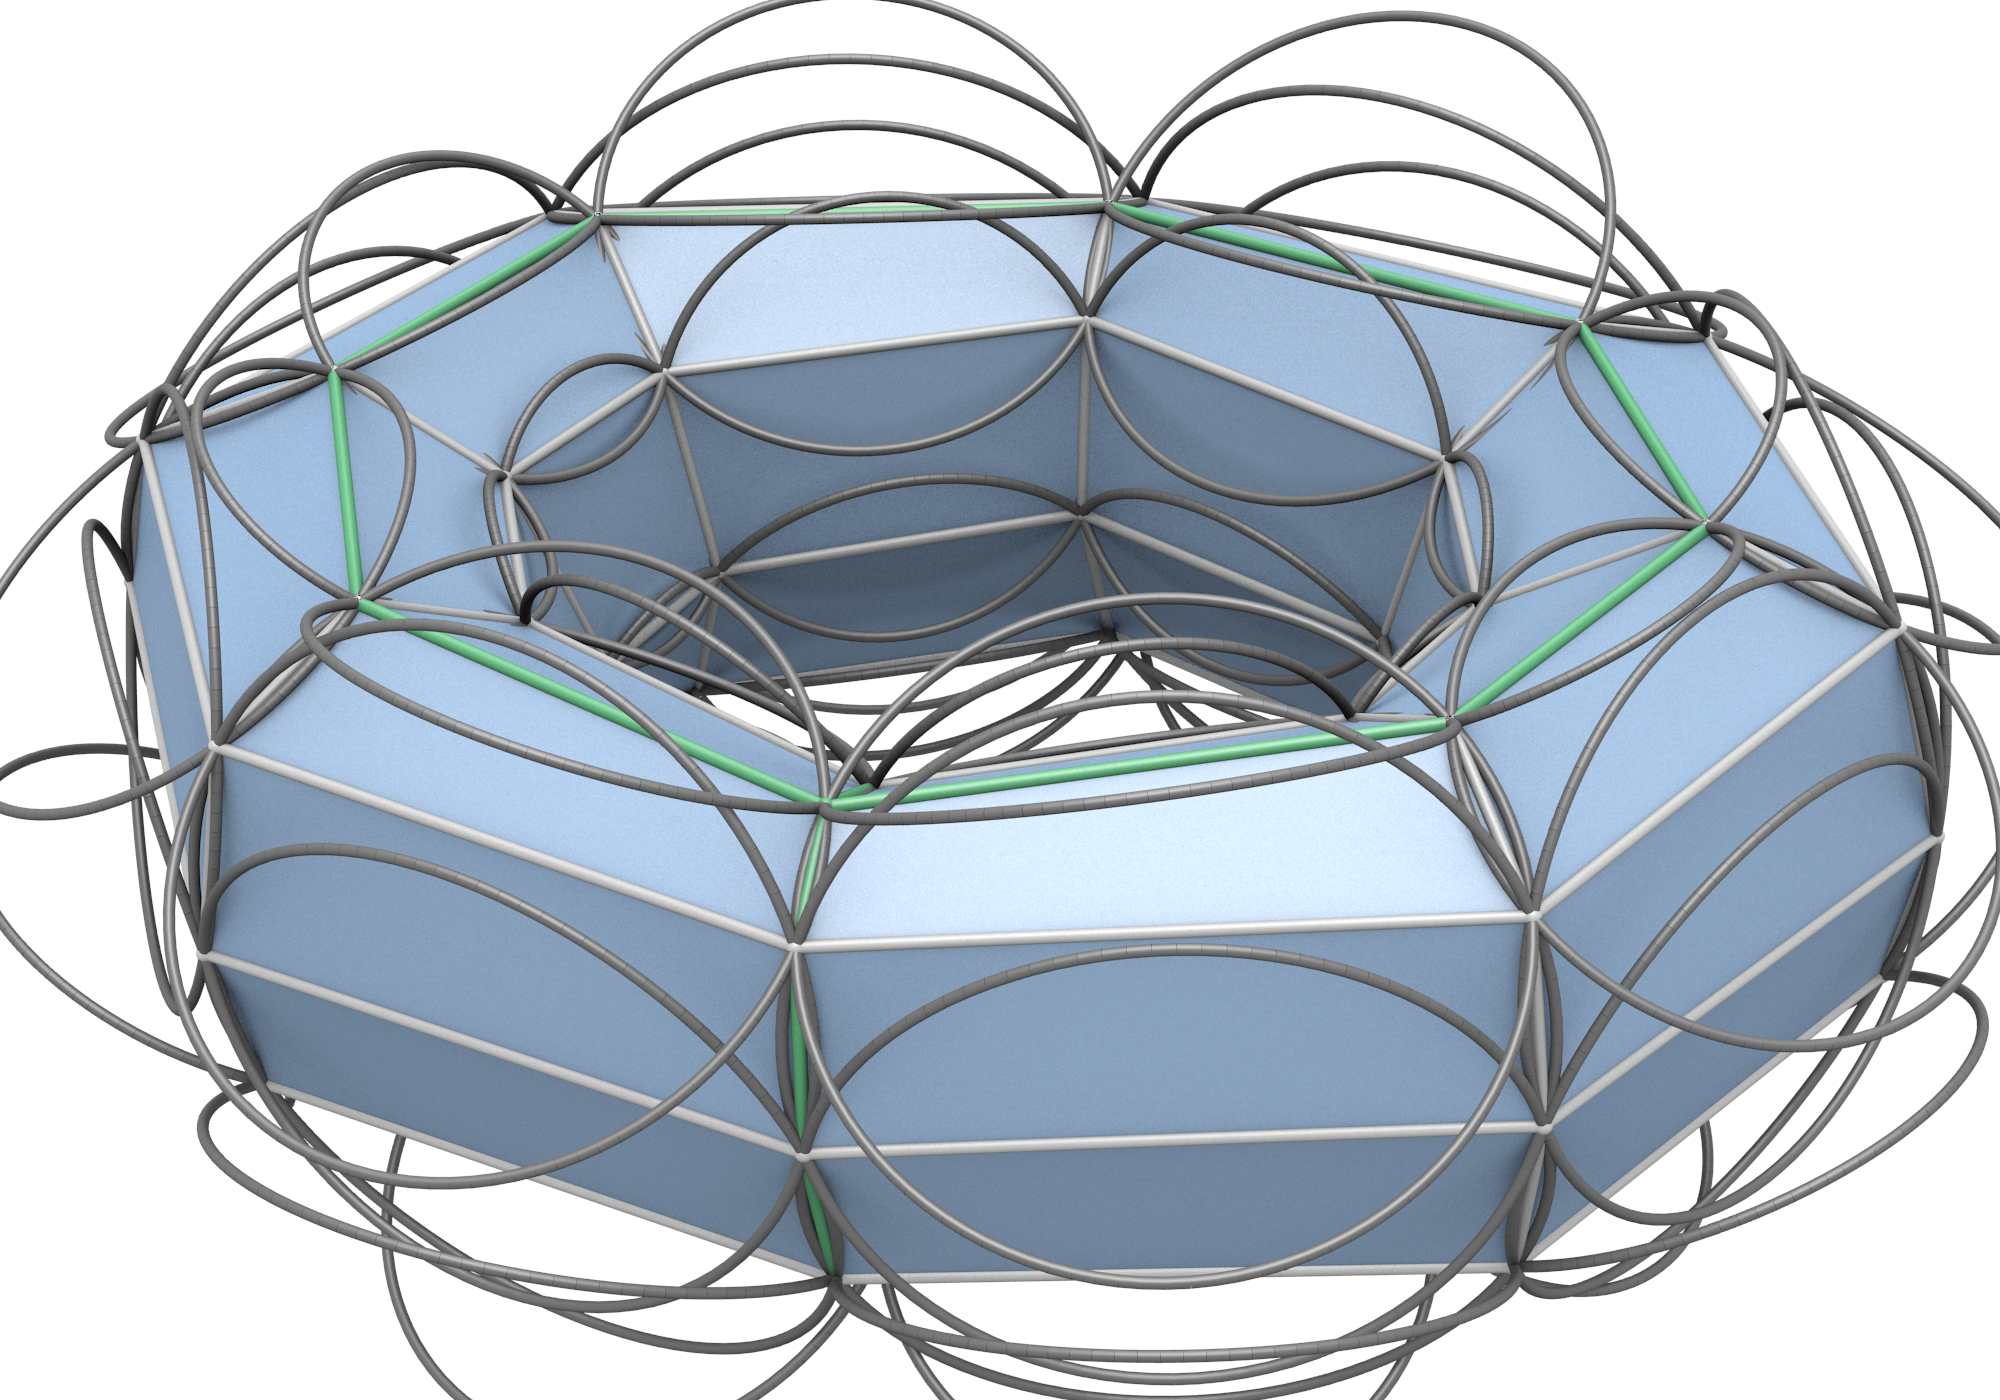
\includegraphics[height=5cm]{torus_cyclic/torus_cyclic_image.pdf}\quad
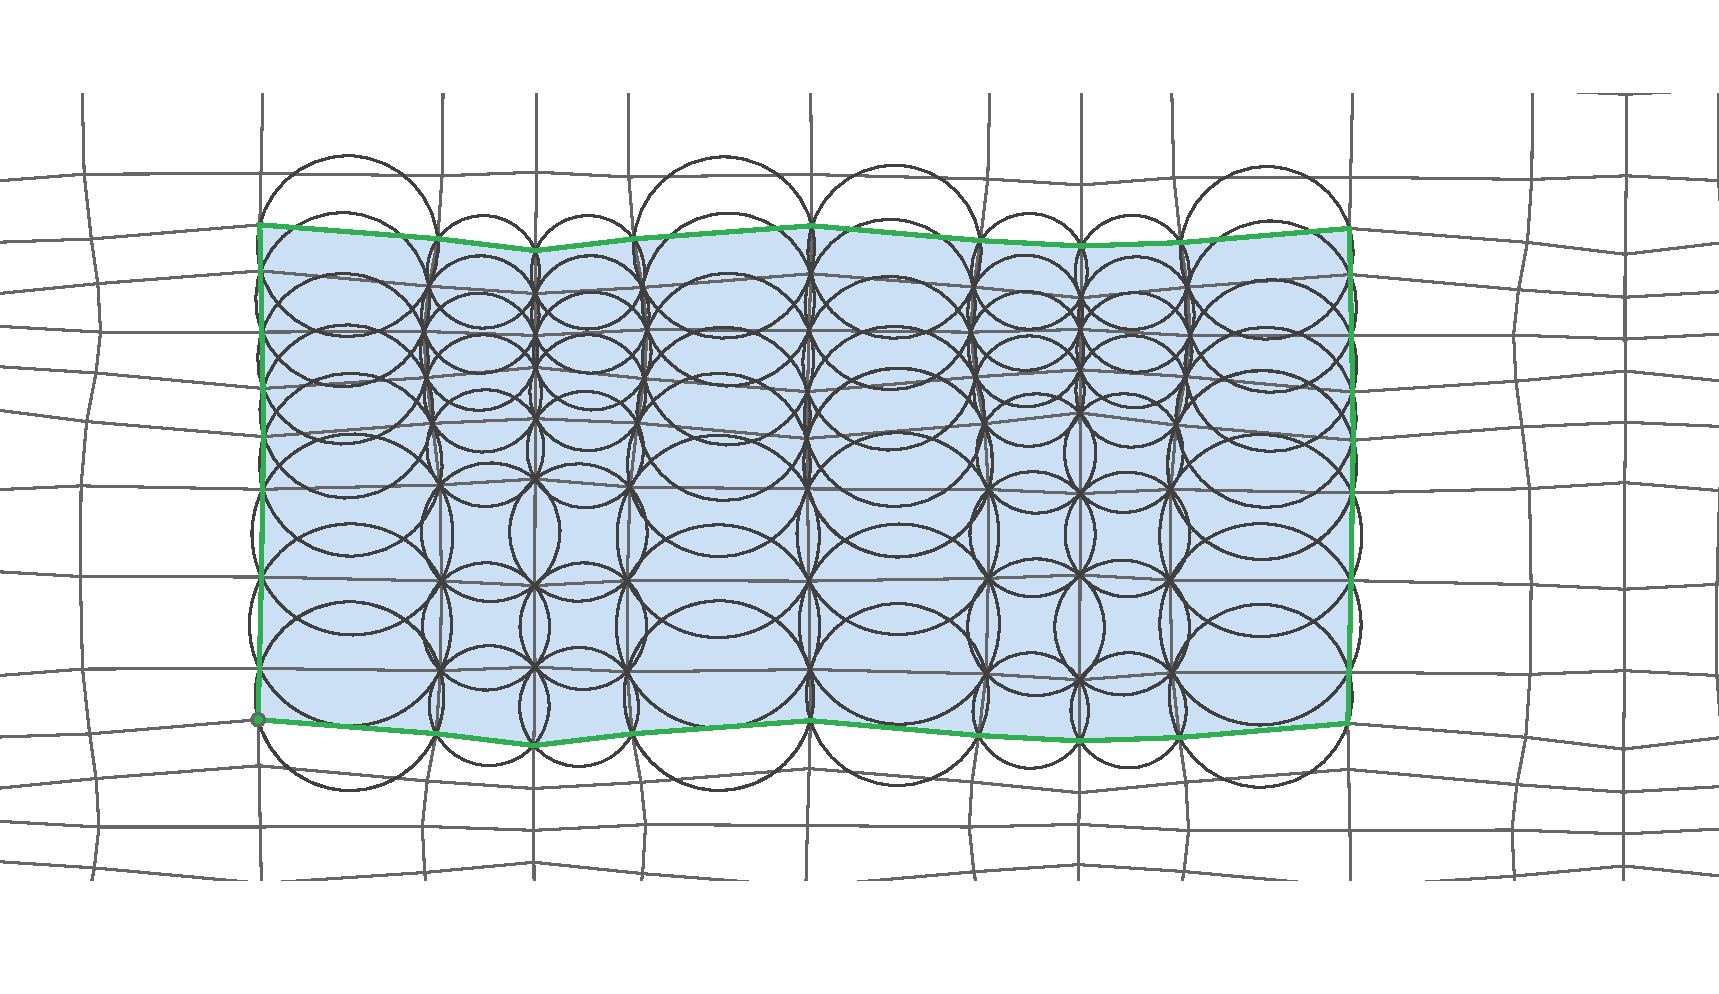
\includegraphics[height=5cm]{torus_cyclic/torus_cyclic_domain.pdf}
}
\setstretch{0.0}{\scriptsize\tt data/torus\_cyclic/torus\_cyclic.xml} 
\caption{
Cyclic discrete conformal map from an embedded torus to the corresponding flat cyclic torus.
Left: Embedding with cuts (green) and circles. 
Right: Flat representation and universal cover with corresponding cuts and circles.
}
\label{fig:torus_cyclic}
\end{figure}

Let $(\Sigma, \ell)$ be a cyclic polyhedral surface with genus $1$ without boundary. 
We solve Problem~\ref{prob:total_angles} to find a euclidean flat metric $\tilde \ell$ with $\Theta_1=2\pi$ for all $i\in V$.
Once we have a solution we can construct the universal cover of $\Sigma$ by laying out the faces into the plane, see Figure~\ref{fig:torus_cyclic}. We construct the uniformizing group, i.e., the group of translations, using an analogous euclidean procedure as described for surfaces of higher genus in Section~\ref{sec:higher_genus}.

\begin{figure}
\centering
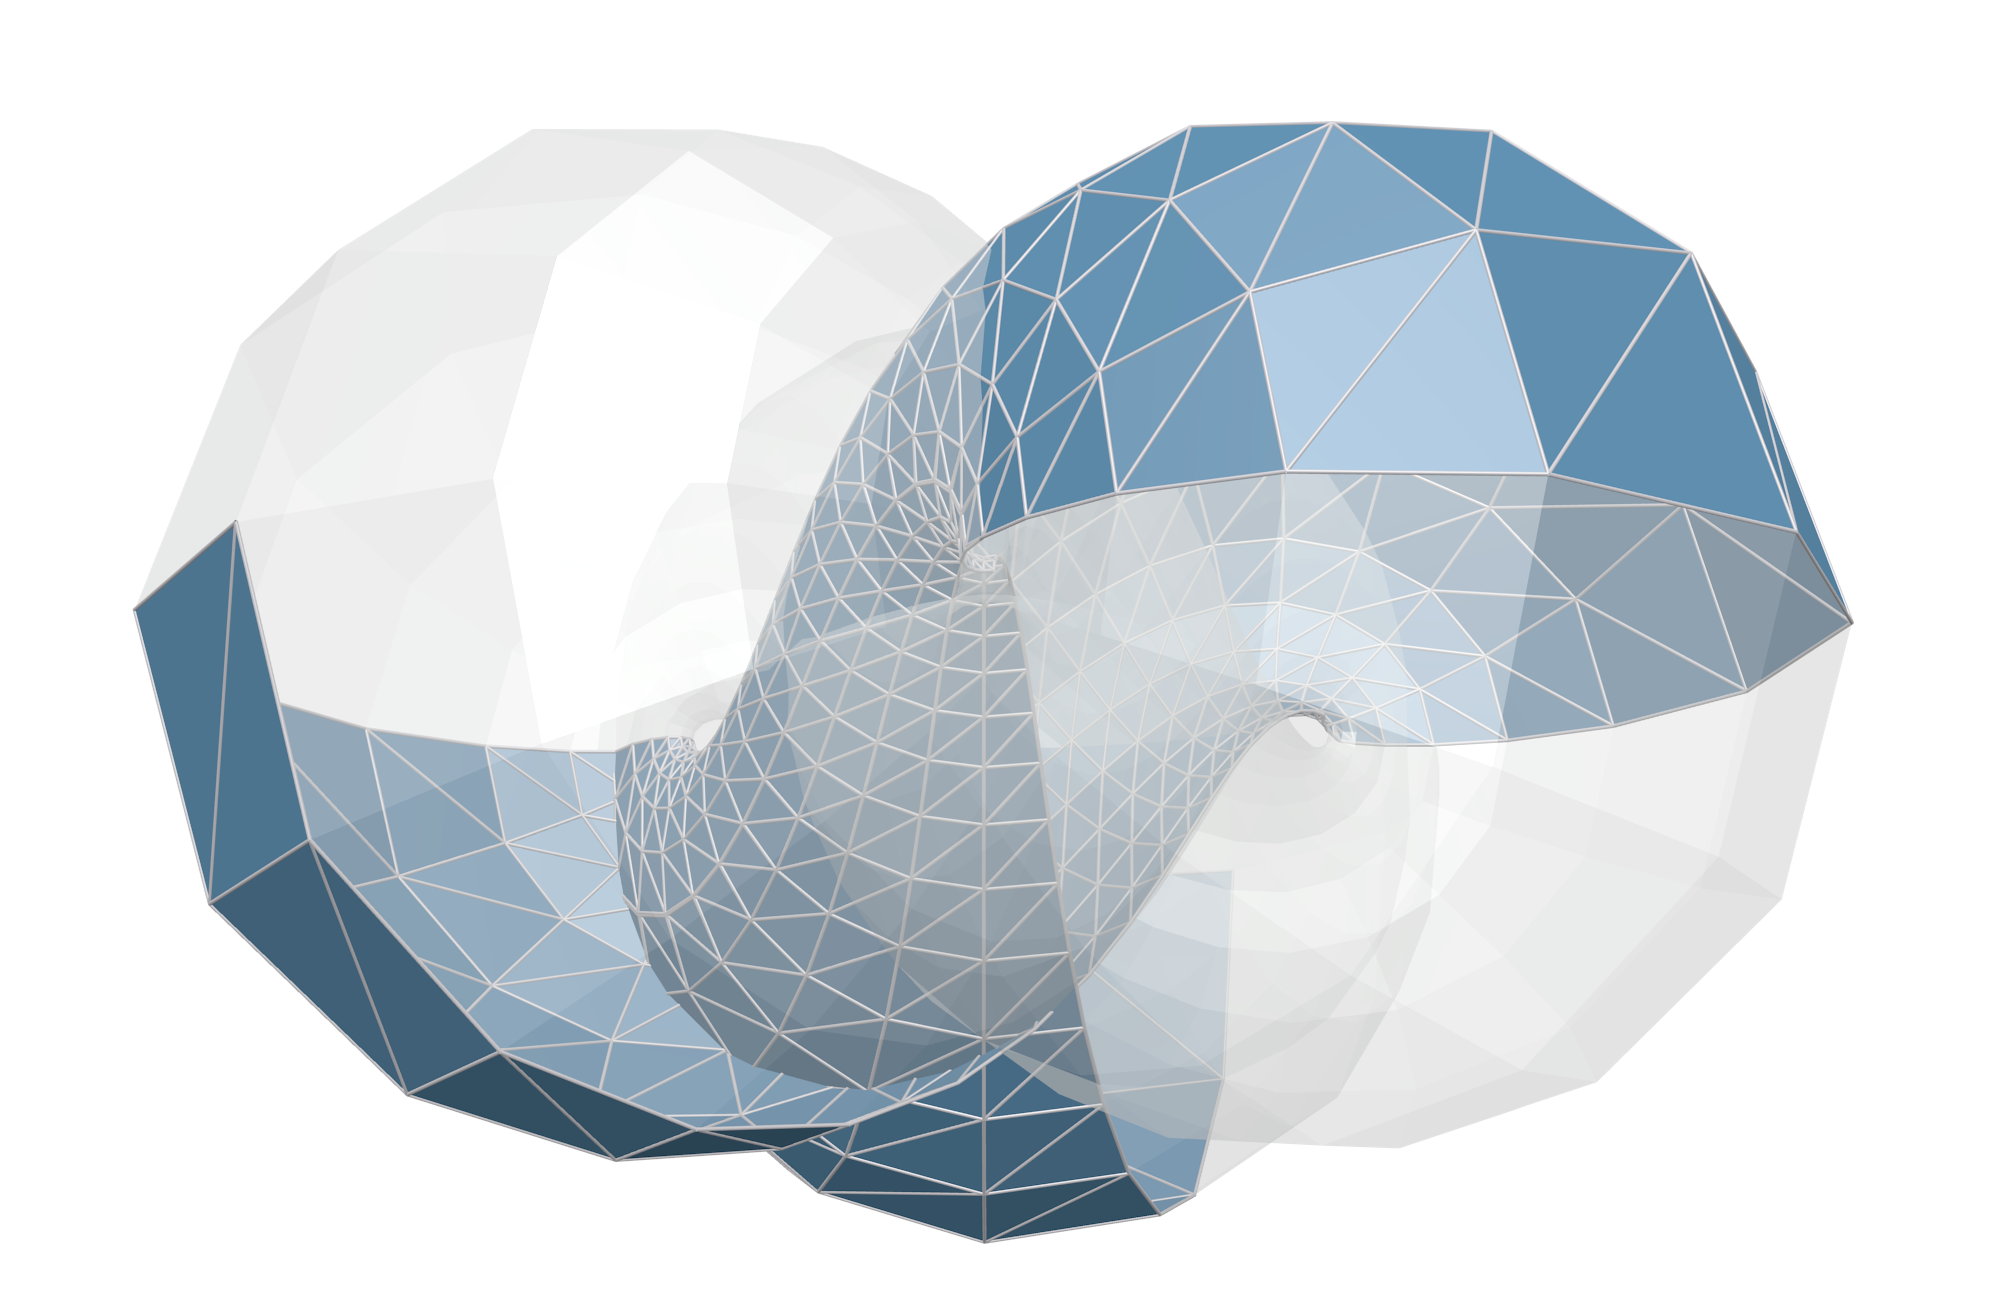
\includegraphics[width=0.48\textwidth,valign=c]{wente_embedding/wente_1240_fundamental.pdf}\hfill
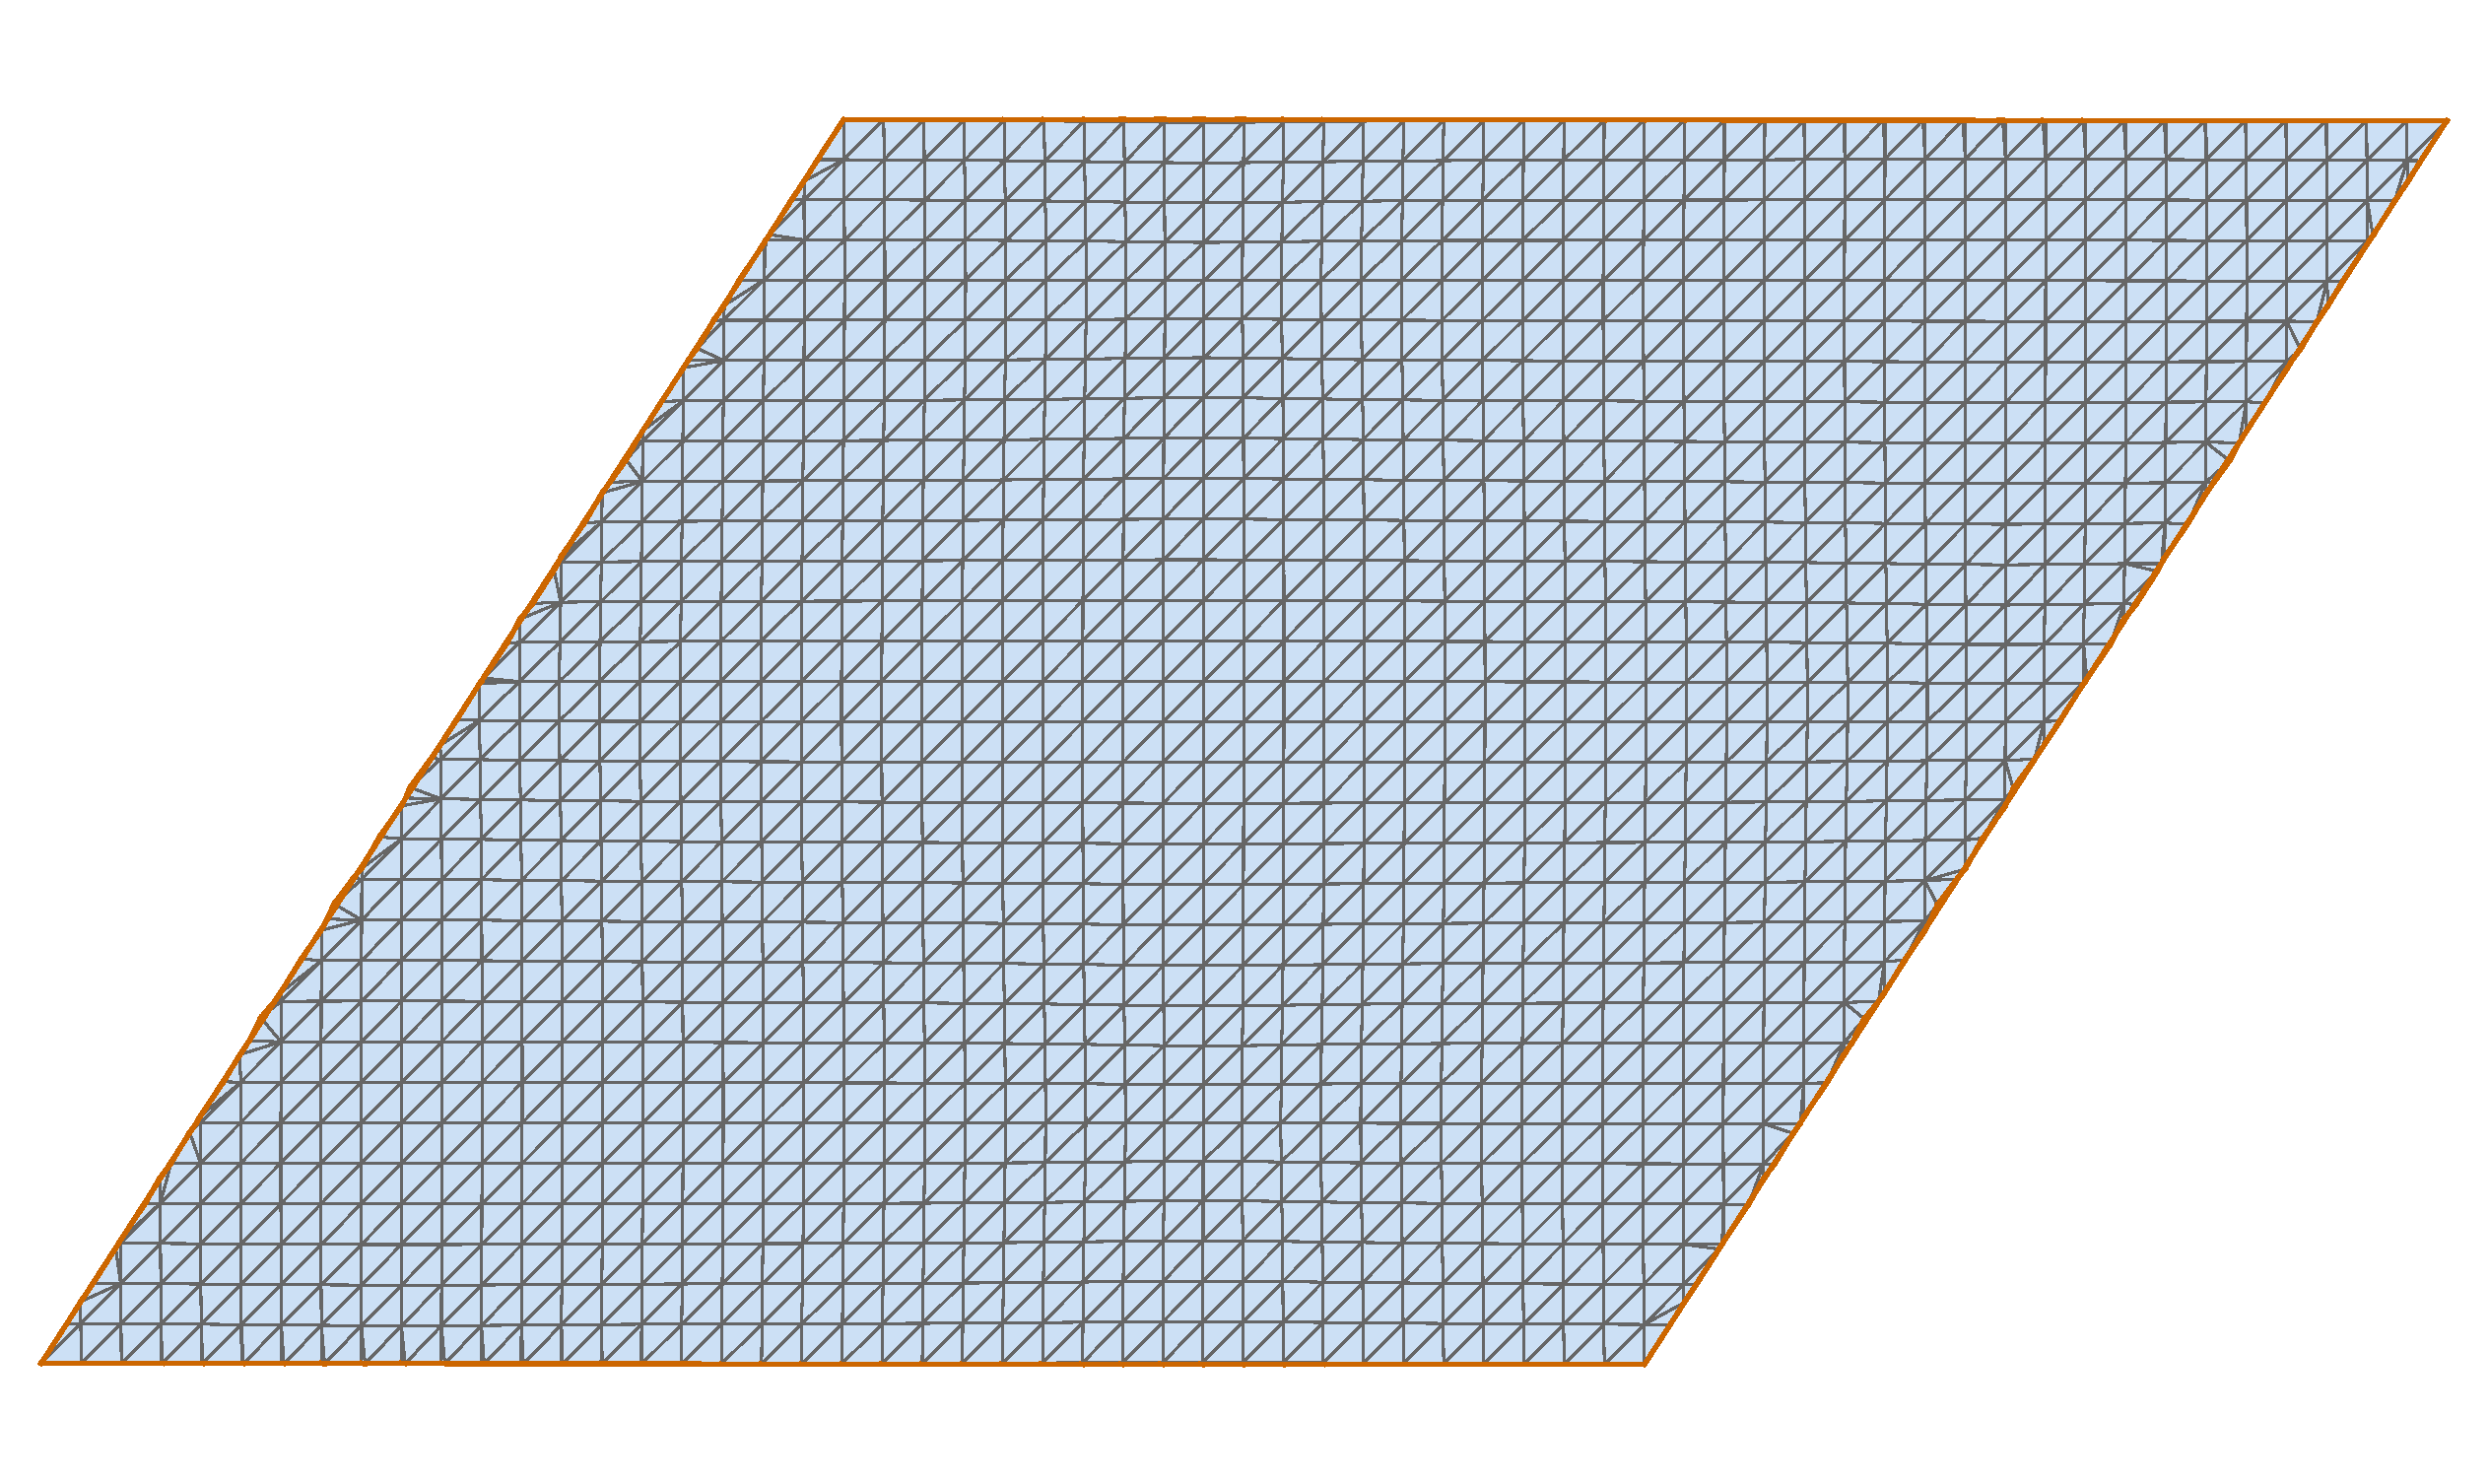
\includegraphics[width=0.48\textwidth,valign=c]{wente_embedding/wente_1240_domain.pdf}
\setstretch{0.5}{\scriptsize\tt data/wente\_embedding/wente\_1240.xml}
\caption{Uniformization of the Wente torus. Discretely sampled conformal immersion (left), domain of uniformization (right). Orange curves indicates the lattice of the flat torus in the domain. The faces of the polyhedral surface are approximate conformal squares. In the discrete uniformization their images are approximately squares, as it should be.}
\label{fig:wente_torus_embedded}
\end{figure}

As a first test we investigate the behavior of discrete conformal maps on the discretization of a conformal immersion of the Wente torus \cite{wente1986}, Figure~\ref{fig:wente_torus_embedded}. 
The modulus of the Wente torus has been calculated reliably before \cite{Heil95} as $\tau \approx 0.41300+0.91073i$.
We calculate a the modulus of the discretized surface as $\tilde \tau \approx 0.41341+0.91061i$, see Figure~\ref{fig:wente_torus_embedded}.


\subsection{Tori given by Schottky data}
\label{sec:tori_schottky}
\begin{figure}
\centering
\resizebox{\textwidth}{!}{
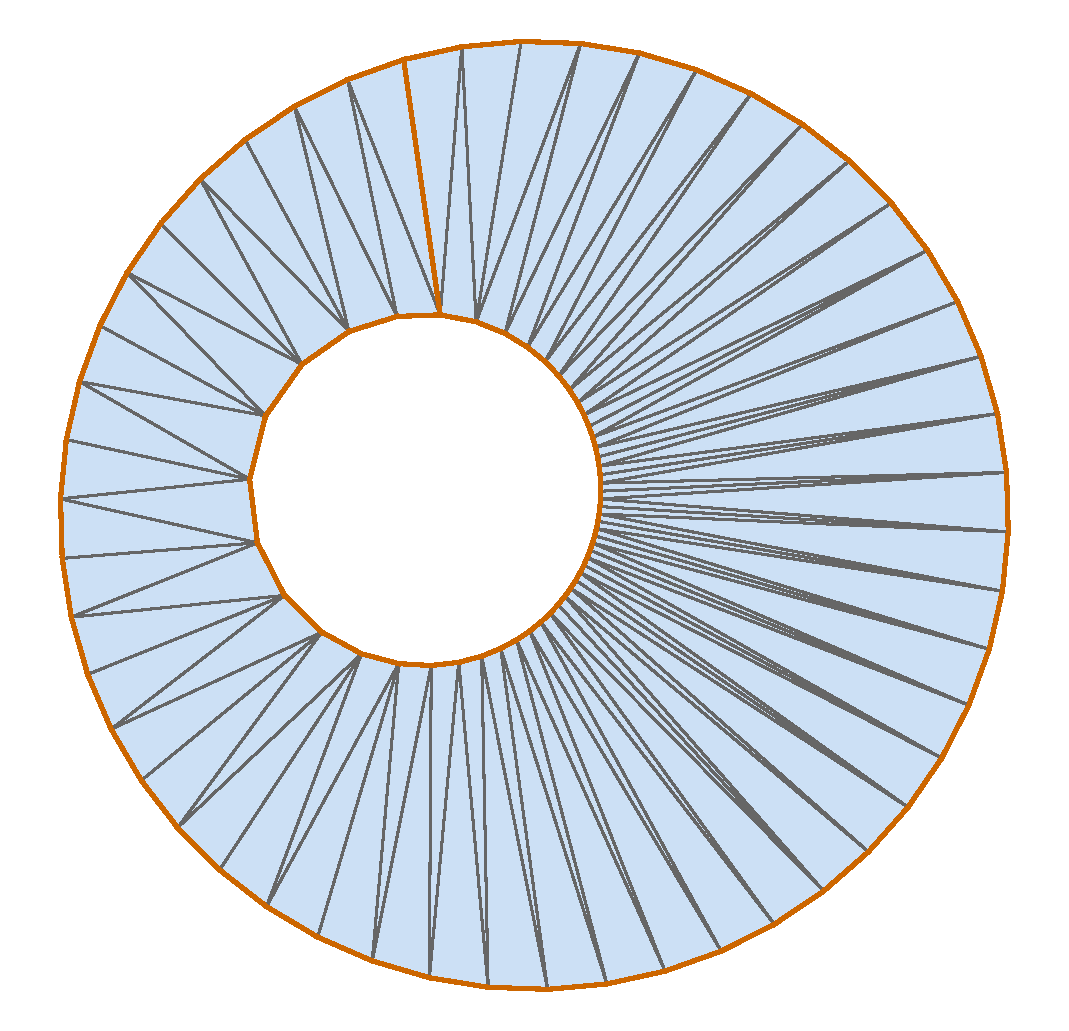
\includegraphics[height=4cm]{data/schottky_g1/res50_image}
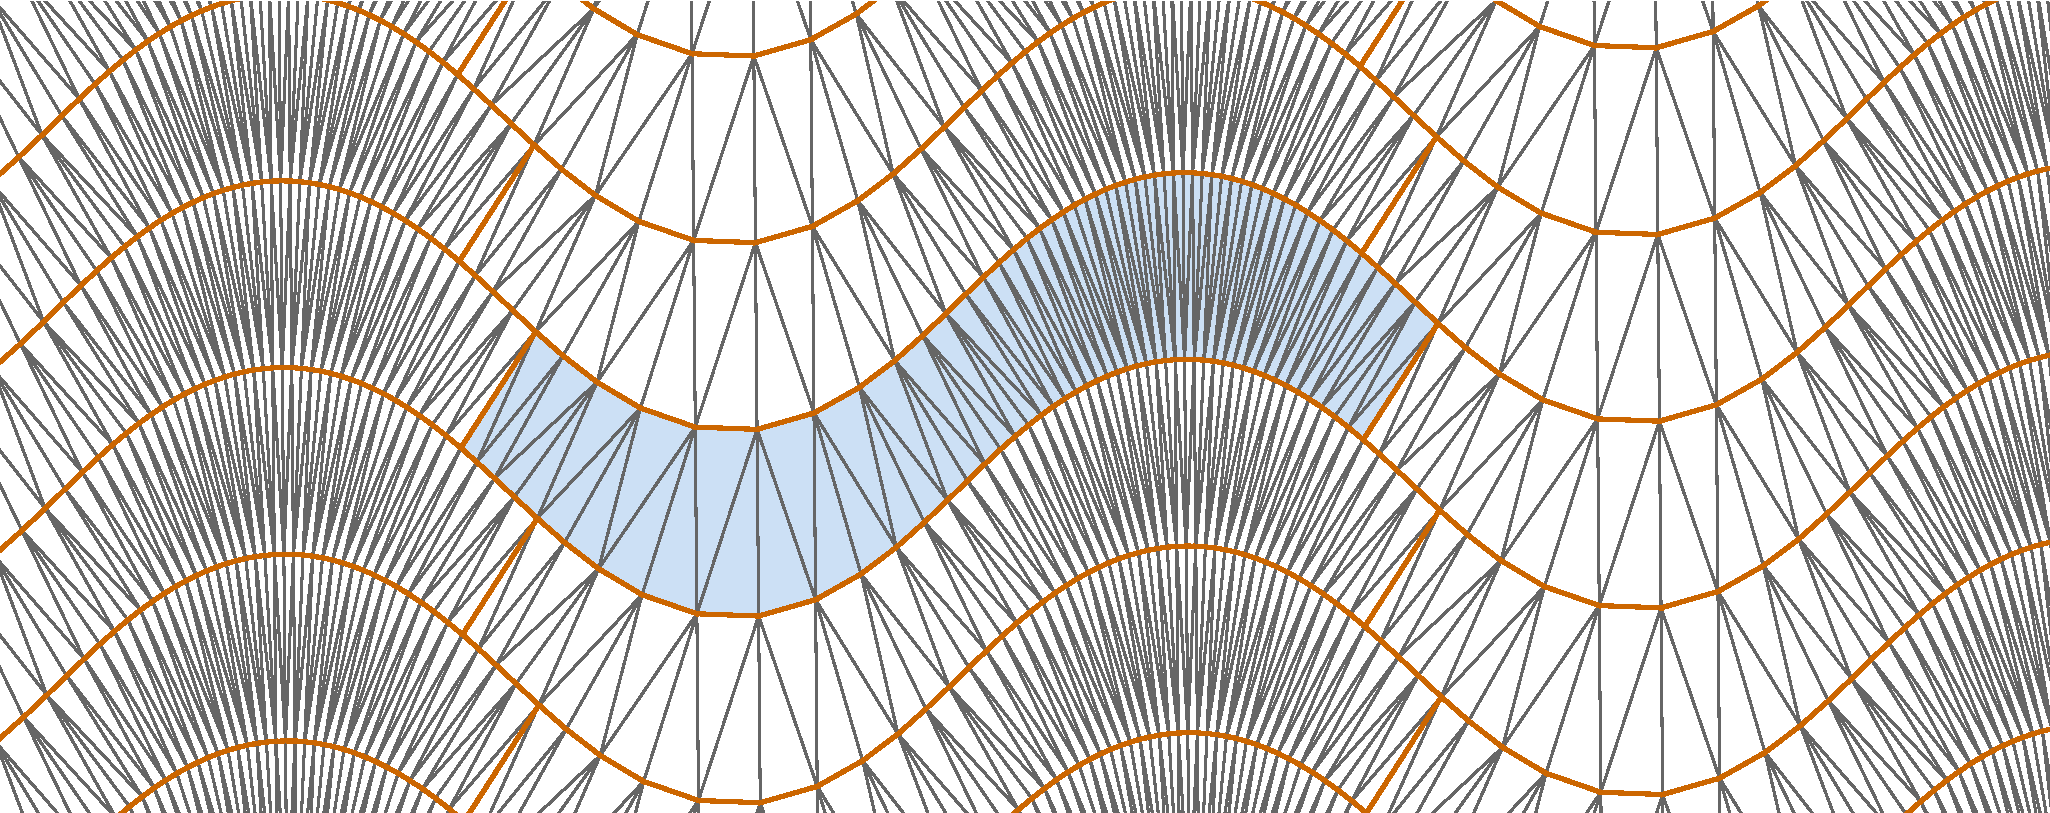
\includegraphics[height=3.9cm]{data/schottky_g1/res50_cover}
}
\setstretch{0.8}{\scriptsize\tt data/schottky\_g1/res50.xml} 
\resizebox{\textwidth}{!}{
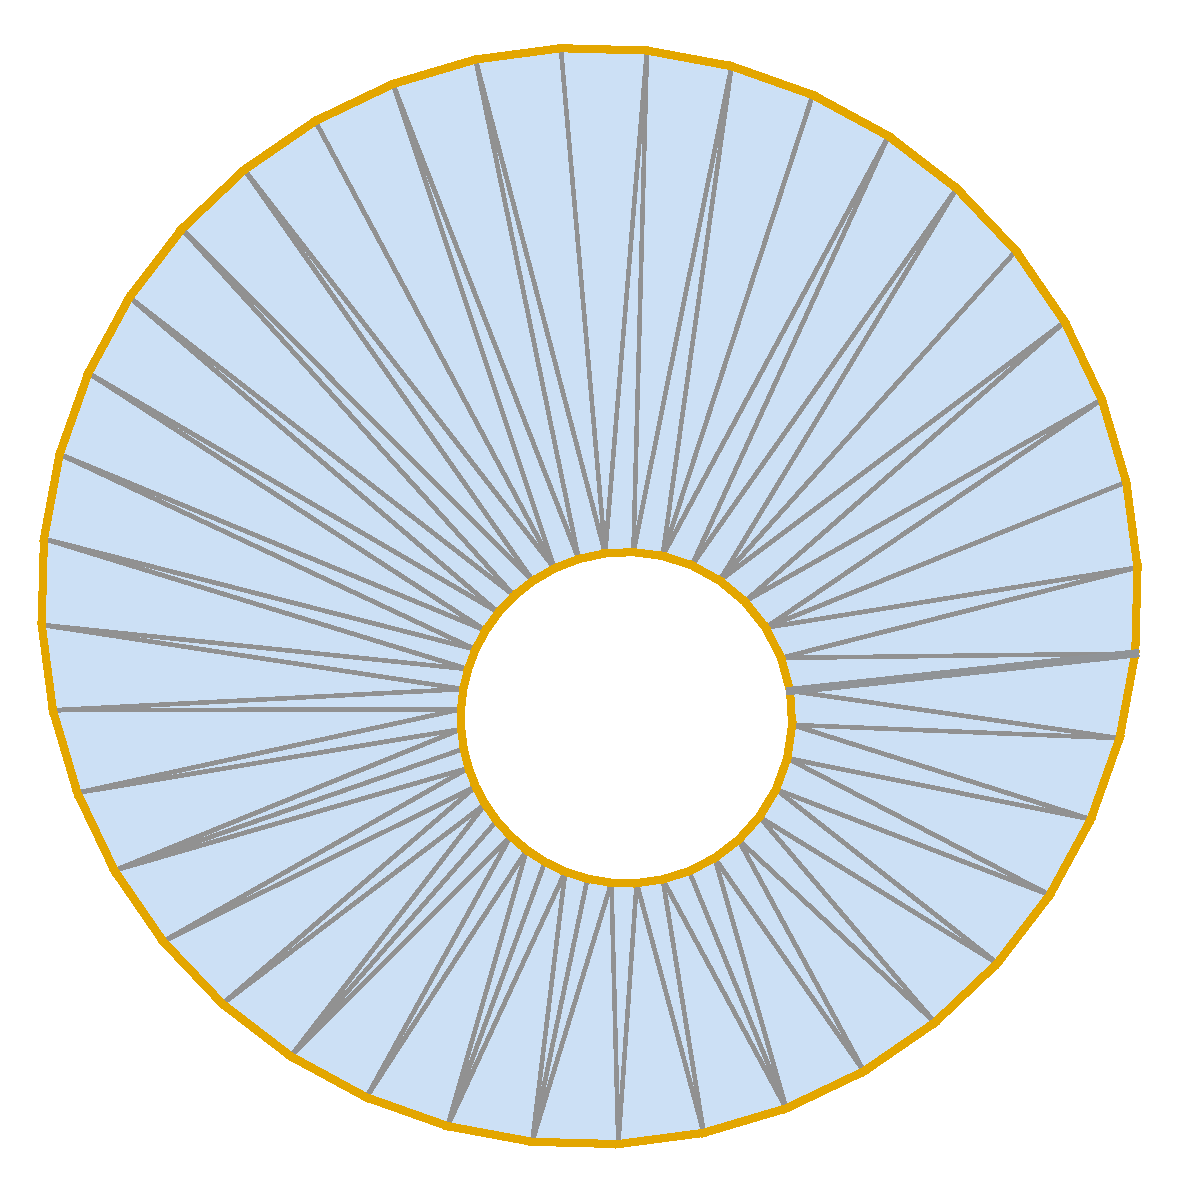
\includegraphics[height=4cm]{schottky_g1/res50_ni_image.pdf}
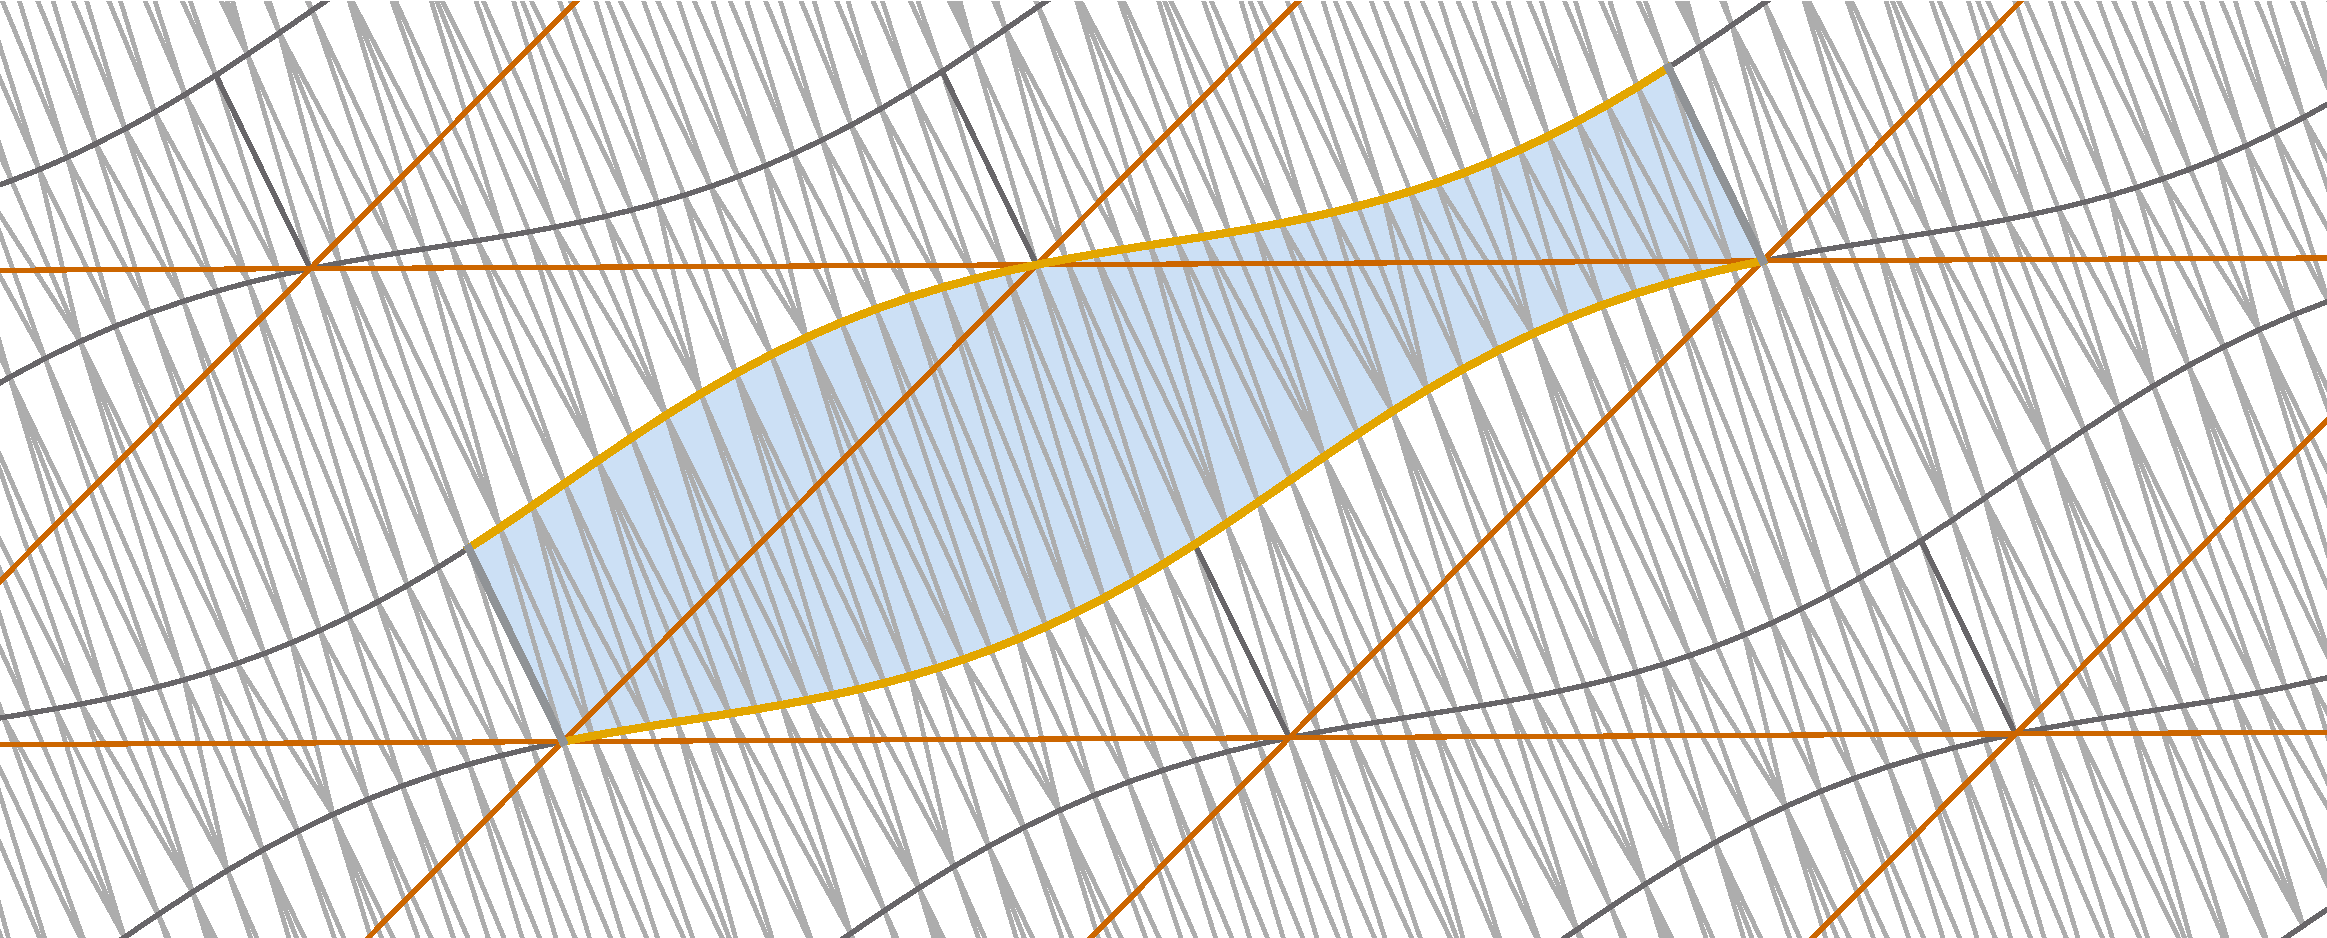
\includegraphics[height=3.9cm]{schottky_g1/res50_ni_cover.pdf}
}
\setstretch{0.8}{\scriptsize\tt data/schottky\_g1/res40\_nonrect.xml}
\caption{
Fundamental domains of triangulated Riemann surfaces of genus $1$ given by Schottky data (left). 
Universal cover and fundamental regions (right). 
Top: For real $\mu=0.3$ we get a rectangle fundamental lattice. 
Bottom: $\mu=0.08+0.01i$ yields a parallelogram.
}
\label{fig:schottky_g1}
\end{figure}

\begin{figure} 
\centering 
\scalebox{1.0}{\input{figures/schottky2.pdf_t}}
\caption{
Schottky group generating a Riemann surface of genus $2$. 
The point at infinity is not contained in any of the circles. 
The fixed points to the transformations $A$ and $B$ lie inside of the circles.
} 
\label{fig:schottky_group}
\end{figure}

Let $C_1,C'_1\ldots,C_g,C'_g$ be disjoint circles in $\hat{\C}$.
\begin{definition} A classical Schottky group $G$ is a Kleinian group with generators $\sigma_1,\ldots,\sigma_g$ satisfying
\begin{equation}
\frac{\sigma_i z - B_i}{\sigma_i z - A_i} = \mu_i \frac{z - B_i}{z - A_i},
\quad\quad\quad 0 < \left|\mu_i\right|<1,
\end{equation}
where $\sigma_i$ maps the exterior of $C_i$ onto the interior of $C'_i$. The points $A_i$ and $B_i$ lie inside the circles $C_i$ and $C'_i$ respectively, see Figure~\ref{fig:schottky_group}.
\end{definition}
Let $G$ be a classical Schottky group. $G$ acts discontinuous on the $\Omega\vcentcolon=\Chat\setminus A$. 
Where $A$ is the limiting set of $G$, i.e., the orbits of $A_i, B_i$ under $G$.
Then $R\vcentcolon=\Omega/G$ is a Riemann surface of genus~$g$.

We discretize the notion of Riemann surface given by Schottky data as follows.
For each pair of circles $(C, C')$ with $\sigma(C) =C'$ we construct two polygons $p_1,\ldots,p_n$ inscribed in $C$ and $p'_1,\ldots,p'_n$ inscribed in $C'$ such that $\sigma(p_i)=p'_i$. E.g., build a regular $n$-gon $C$ and map the points by $\sigma$ onto $C'$.
Triangulate the outside of the circles.
Corresponding edges on $C$ and $C'$ are identified on $R$ but do not have the same length in $\Chat$.
Corresponding edges in $\Chat$ have the same length cross-ratio as this characterization is invariant under M\"{o}bius transformations.
That means we have a unique function $\lcr$ defined on $E$.
We pick a representative metric $\ell$ to feed into the variational principle and calculate the uniformization, see Section~\ref{sec:cross-ratios} and Figure~\ref{fig:schottky_g1}.
Note that the lengths $\ell$ that are a representative for $\lcr$ is not a metric in general, i.e., the polygon inequalities might be violated. 
We will however find the correct minimizer as the functional is defined even for invalid metrics, see Section~\ref{sec:convexity_extension}.

For tori we have only one generator and one pair of circles. 
The general case of arbitrary genus leads to hyperbolic uniformization groups, i.e. Fuchsian groups, and is treated in Section~\ref{sec:schottky}.

\subsection{Tori given as algebraic curves}
\label{sec:discrete_algebraic_curves}

\begin{figure}
\centering
\resizebox{\textwidth}{!}{
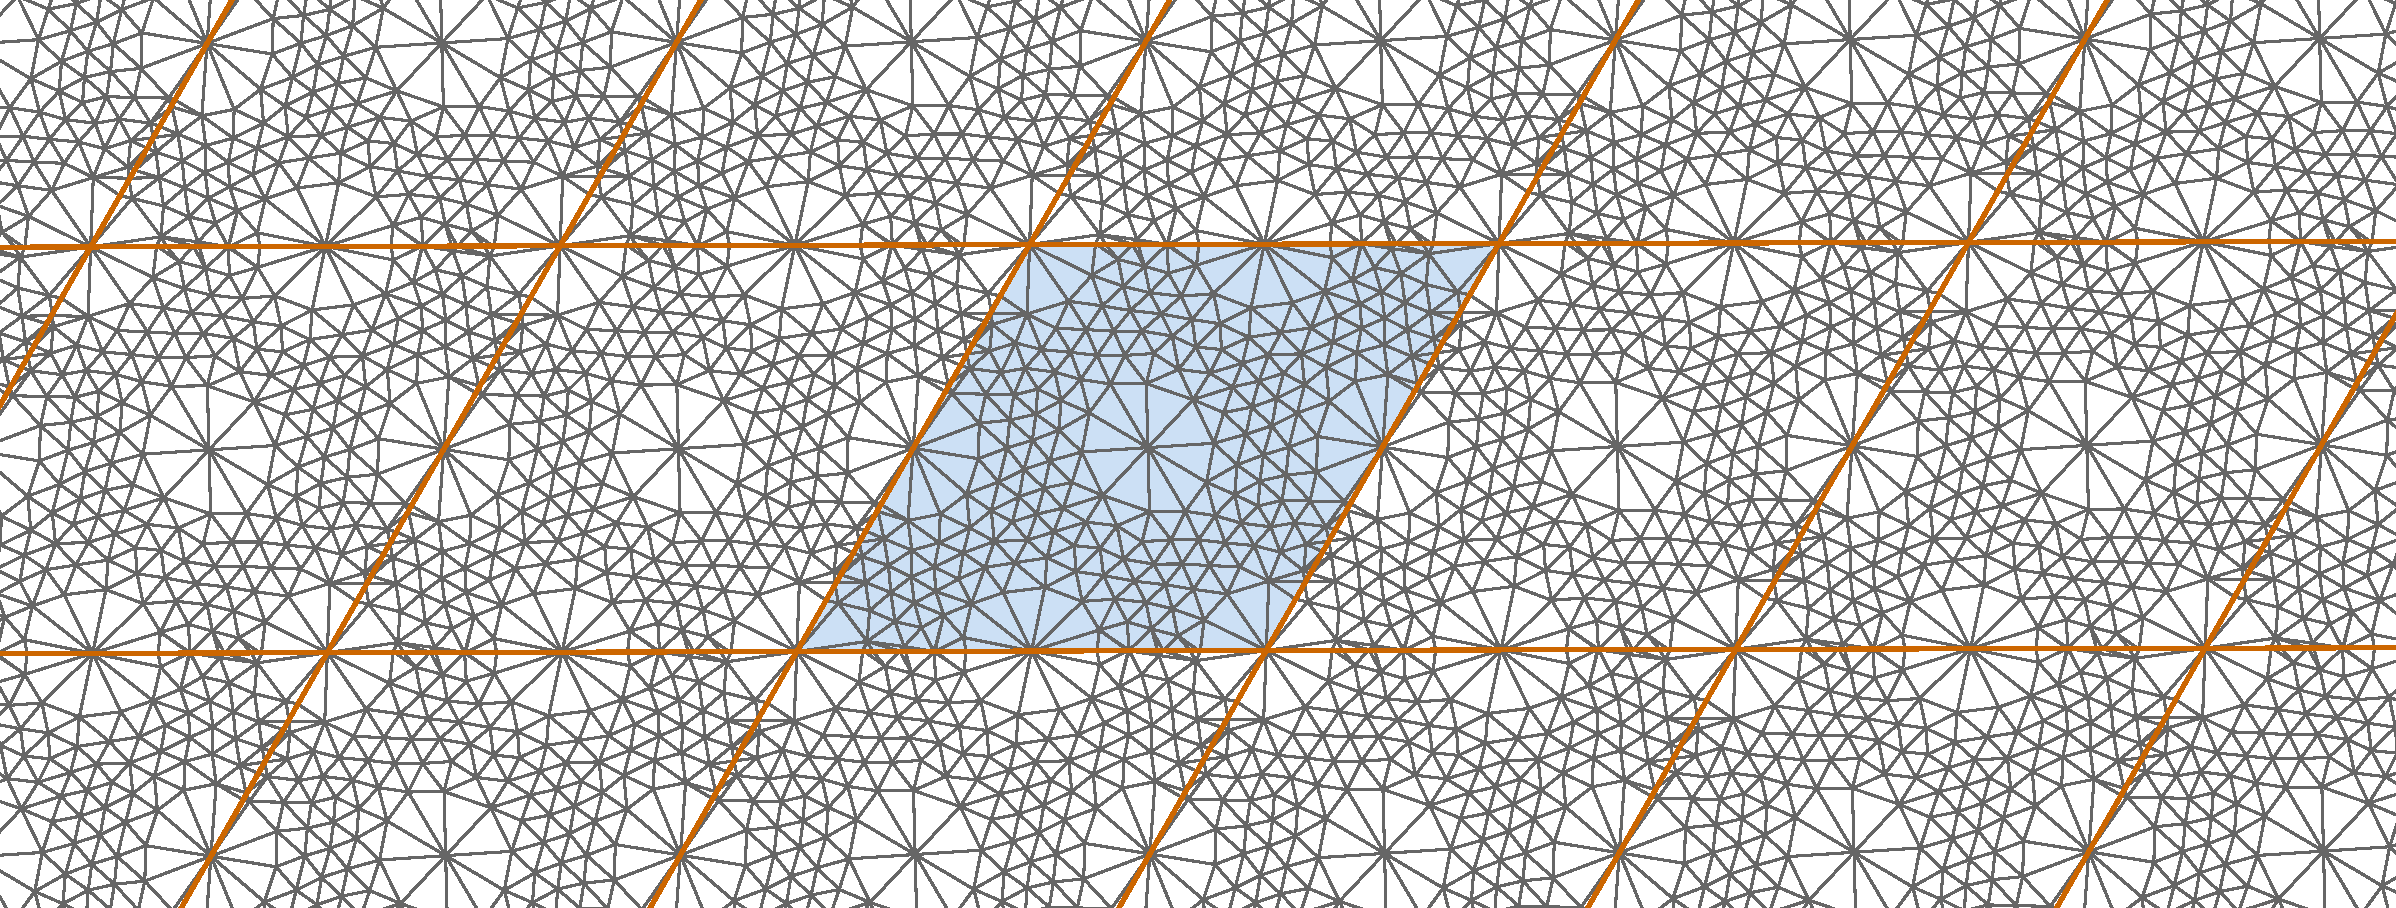
\includegraphics[width=0.5\textwidth]{elliptic_curves/tetrahedron.pdf}
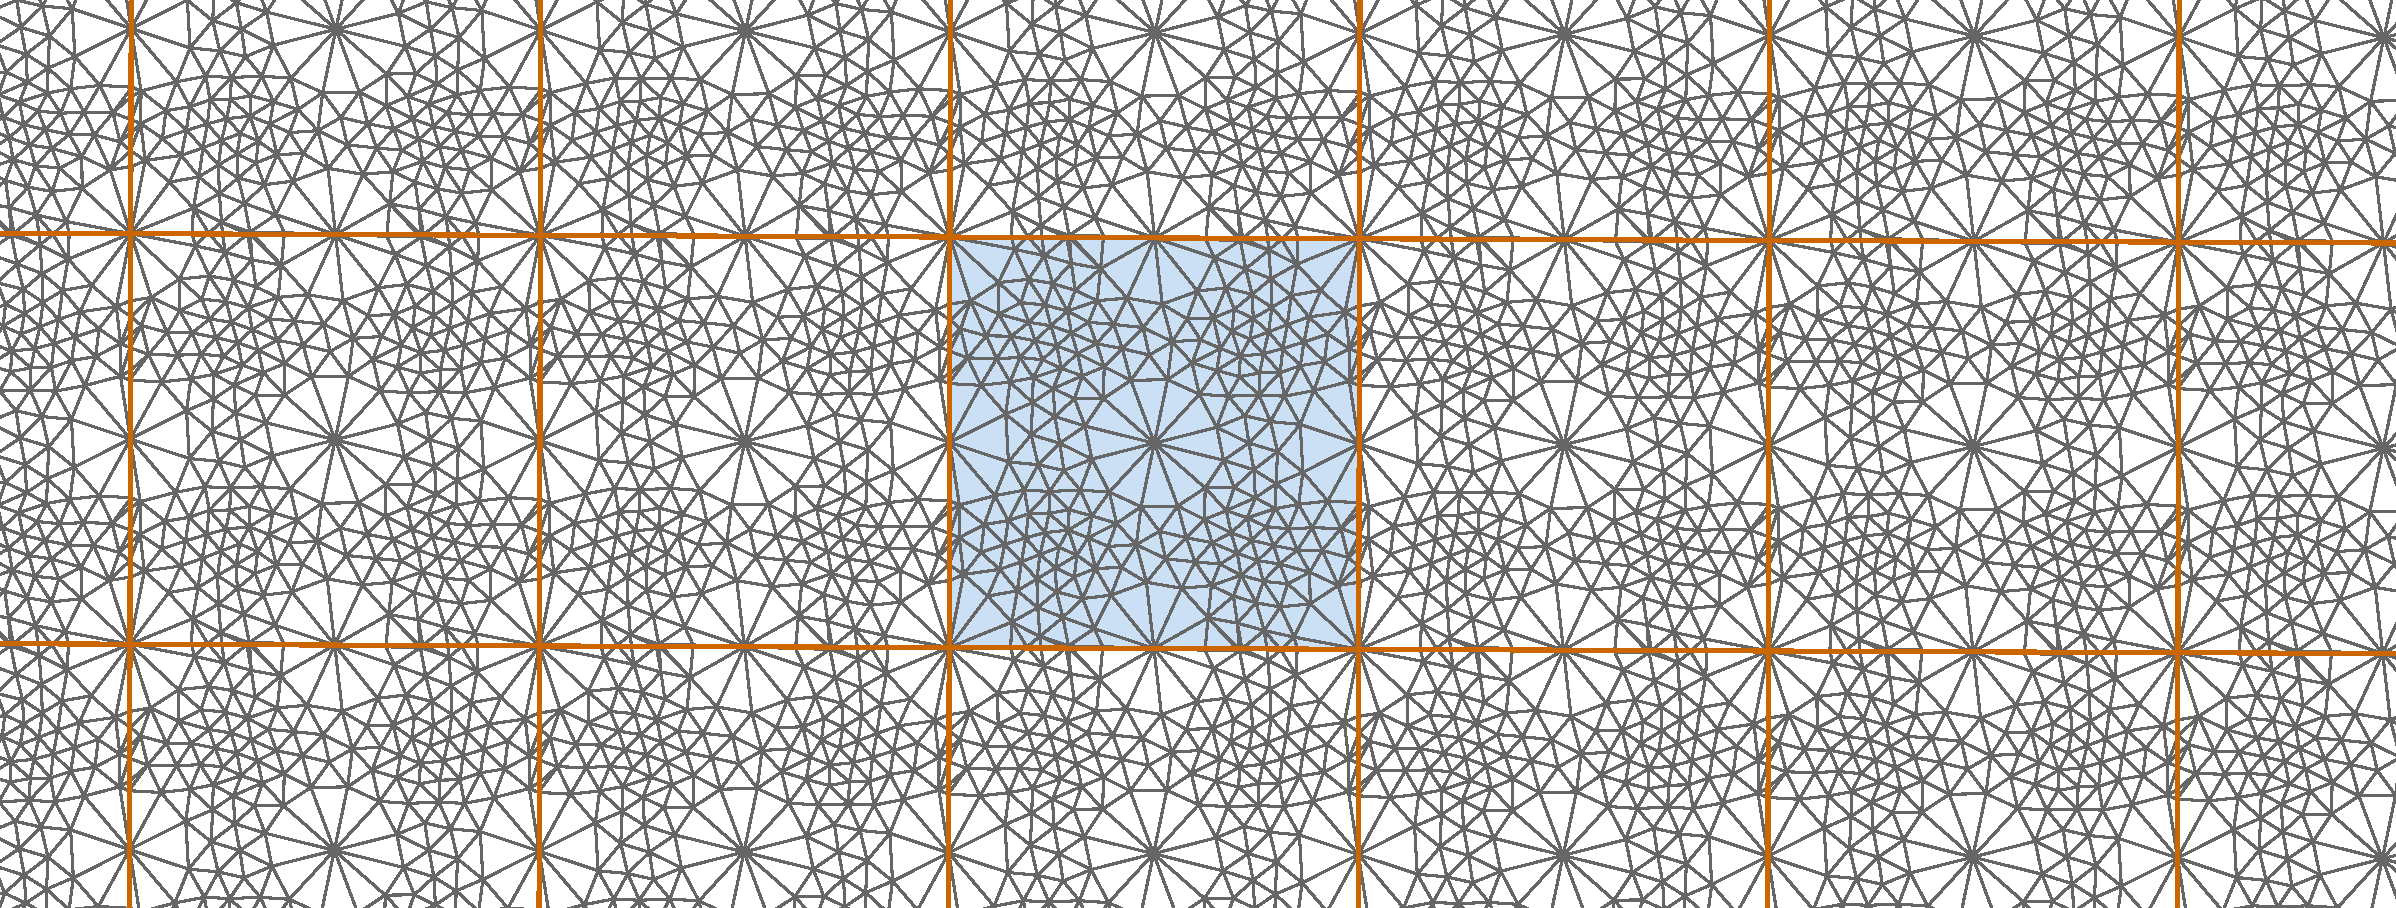
\includegraphics[width=0.5\textwidth]{elliptic_curves/square.pdf}
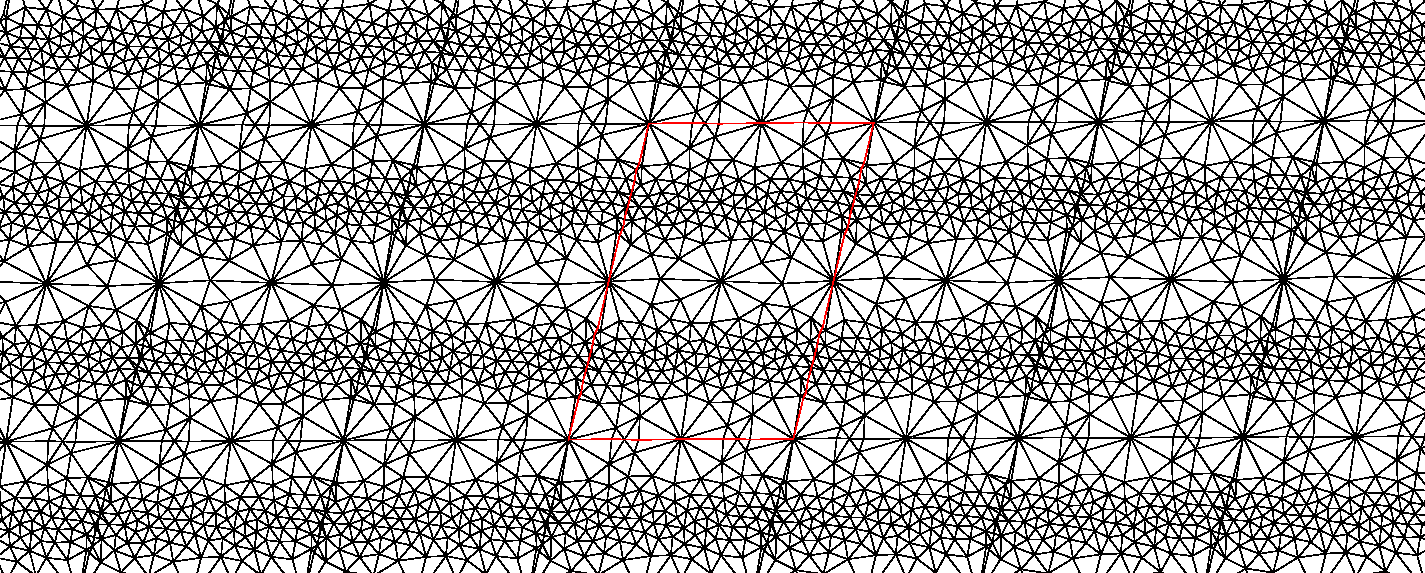
\includegraphics[width=0.5\textwidth]{elliptic_curves/generic.pdf}
}
\setstretch{0.8}{\scriptsize\tt data/elliptic\_curves/\{tetrahedron|square|generic\}.xml}
\caption{Discrete versions of elliptic functions. Left: The lattice $\tau=\frac{1}{2}+\frac{\sqrt 3}{2}i$. On the sphere the branch points form a regular tetrahedron. Middle: $\tau=i$, branch points on $\hat \C$ are located in a square on the equator. Right: Branch points in general position.}
\label{fig:p_functions}
\end{figure}

Every Riemann surface is conformally equivalent to an algebraic curve
\[C=\left\{(\lambda,\mu)\in \C^2 \mid \mathcal P(\lambda,\mu)=0\right\}\]
where $\mathcal P$ is an irreducible polynomial.
This curve in turn can be represented as branched covering of the Riemann sphere $\hat{\C}$ with branch points at locations $\lambda_i$ with \[\frac{\partial\mathcal P}{\partial \mu}\Bigr|_{\lambda=\lambda_i} = 0.\]
In the discrete setting we represent discrete algebraic curves as triangulations of the respective branched covering of $\S^2$.
We only cover 2-sheeted coverings here as this includes our main examples, i.e., elliptic curves and hyperelliptic curves, see also Section~\ref{sec:hyperelliptic}.

We construct a triangulation of such a 2-sheeted covering as follows.
Let $S$ be a Riemann surface with genus $g\geq 1$.
Let $\lambda_1,\ldots,\lambda_{2g+2}\in \hat\C$ be the branch points of the corresponding algebraic curve.
Let $\sigma :\hat\C\to\S^2$ be the stereographic projection mapping $\infty$ to the north pole of the sphere, $0$ is mapped to the south pole, and the unit circle is mapped to the equator.
Choose points $p_1,\ldots,p_n\in\S^2$ such that the convex hull $P$ of $\{\sigma\lambda_1,\ldots,\sigma\lambda_{2g+2},p_1,\ldots,p_n\}$ forms a convex polyhedron.
In particular $P$ forms a cyclic polyhedron.

Take a second copy $\hat P$ of $P$. $P$ and $\hat P$ will serve as the first and second sheet of the 2-sheeted covering.
Find non-intersecting edge paths $\gamma_1,\ldots,\gamma_{g+1}$ each connecting a pair of branch points on $P$ and simultaneously on $\hat P$.
Note that the resulting surface does not depend on the choice of $\gamma$.
We cut the two sheets along $\gamma_1,\ldots,\gamma_{g+1}$ and identify the sides of the cuts transversely across $P$ and $\hat P$.
By this procedure the end points $\lambda$ are identified between the two sheets $P$ and $\hat P$.

We use this construction to calculate discrete versions of elliptic functions.
We start with the branch data $\lambda_1,\ldots,\lambda_{4}$ and create a triangulated two-sheeted cover branched at the given $\lambda$s, see Figure~\ref{fig:p_functions}.


\begin{figure}
\centering
\resizebox{\textwidth}{!}{
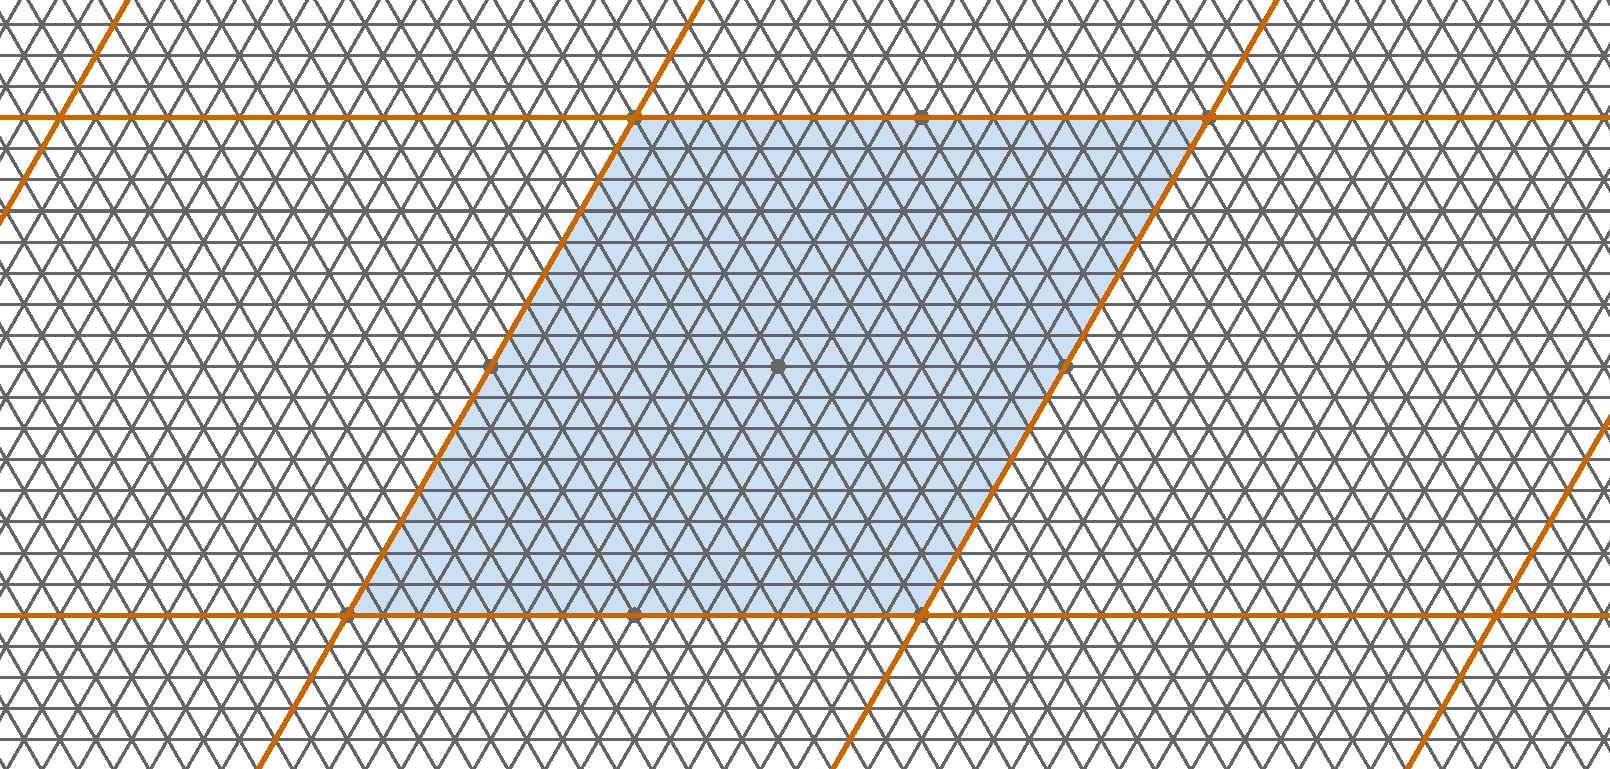
\includegraphics[height=4.5cm]{elliptic_tetrahedron_uniform/tetrahedron_uniform_domain.pdf}
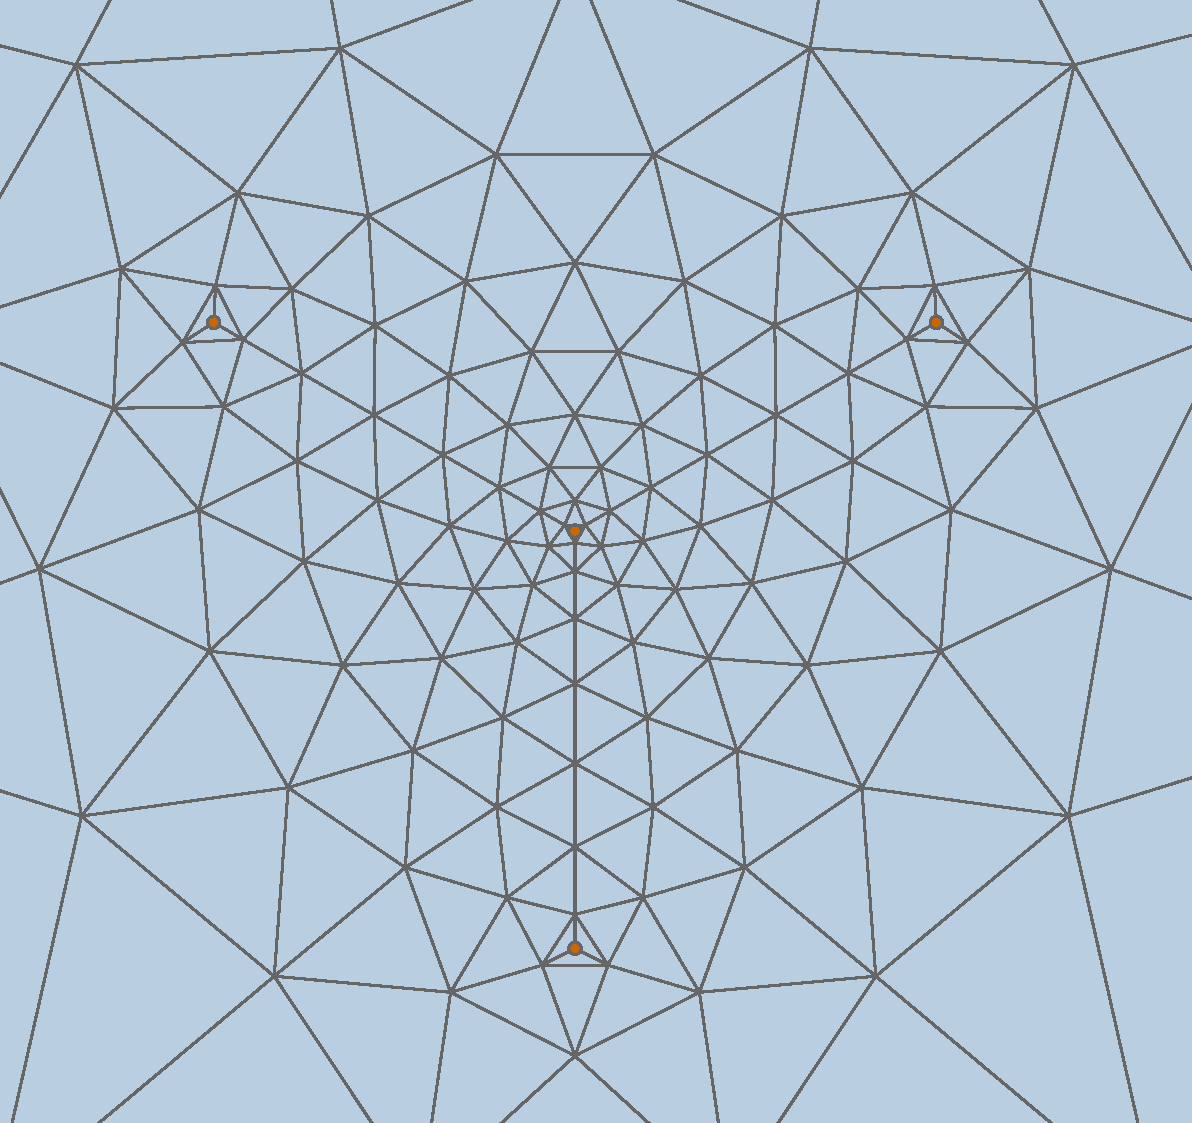
\includegraphics[height=4.5cm]{elliptic_tetrahedron_uniform/tetrahedron_uniform_image.pdf}
}
\setstretch{0.8}{\scriptsize\tt data/elliptic\_tetrahedron\_uniform/tetrahedron\_uniform\_branched.xml}
\caption{
Map from the torus $\tau=\frac{1}{2}+\frac{\sqrt 3}{2}i$ to $\Chat$. 
Left: Regular subdivision of the elliptic lattice. 
Right: Two-sheeted image of the map, both sheets coincide due to the regular subdivision. 
Red point correspond to the four branch points under stereographic projection.
On $\Chat$ the branch points have the symmetry of a tetrahedron.
} 
\label{fig:wente_elliptic}
\end{figure}

\begin{figure}
\centering
\resizebox{\textwidth}{!}{
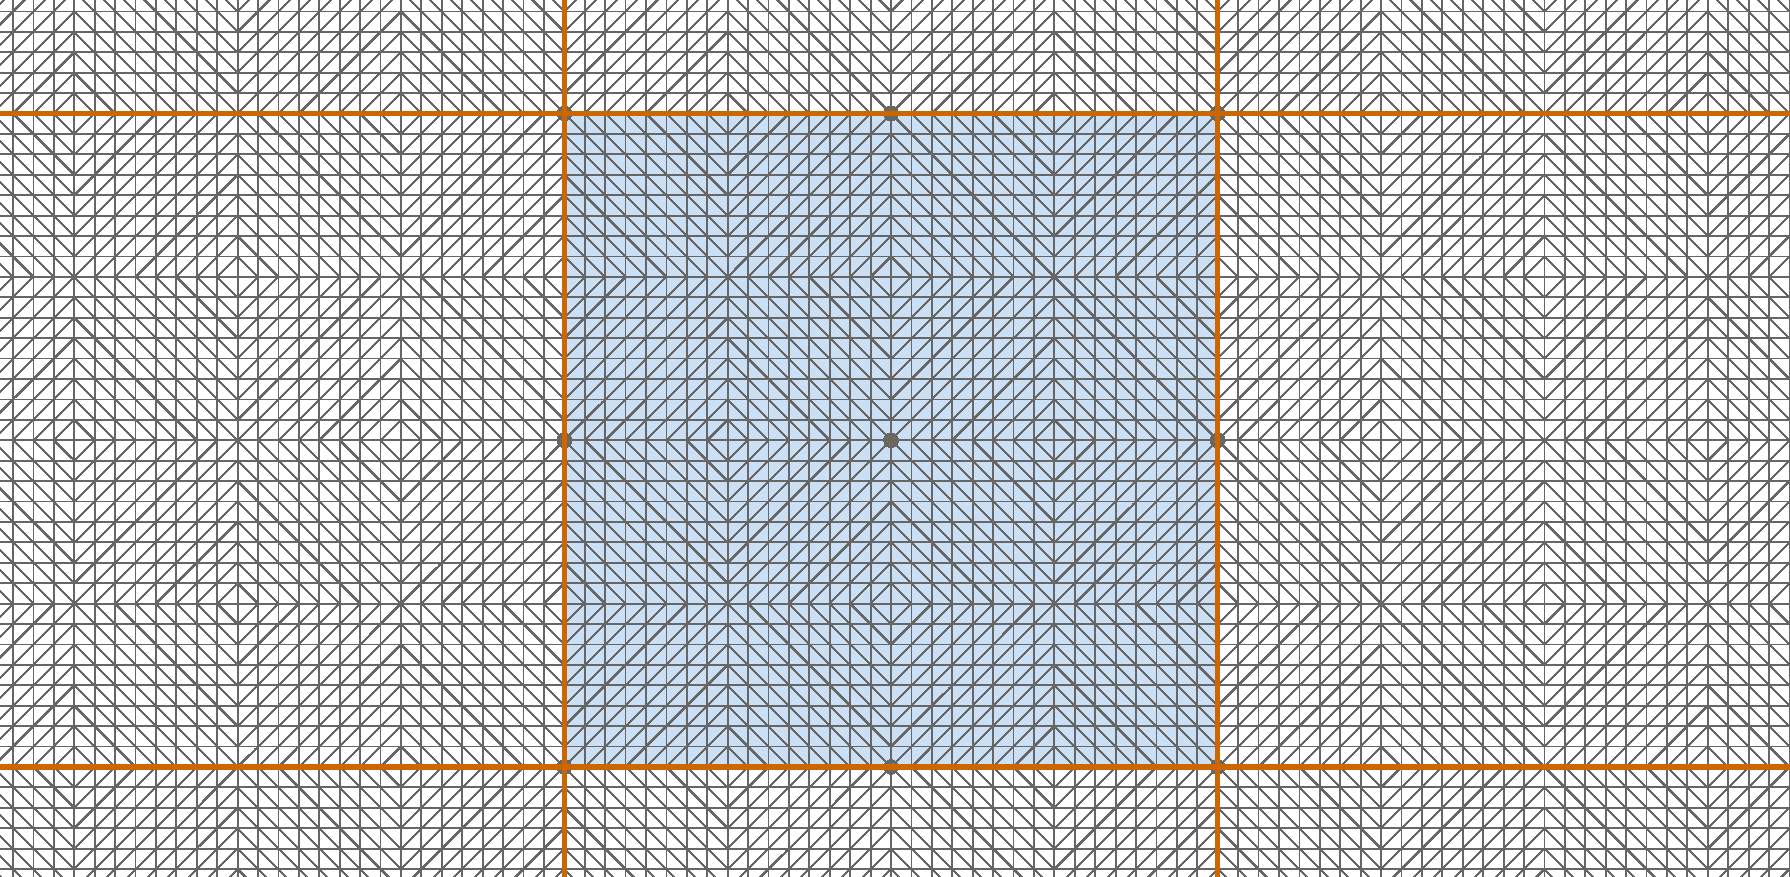
\includegraphics[height=4.7cm]{elliptic_square_uniform/square_uniform_fine_domain.pdf}
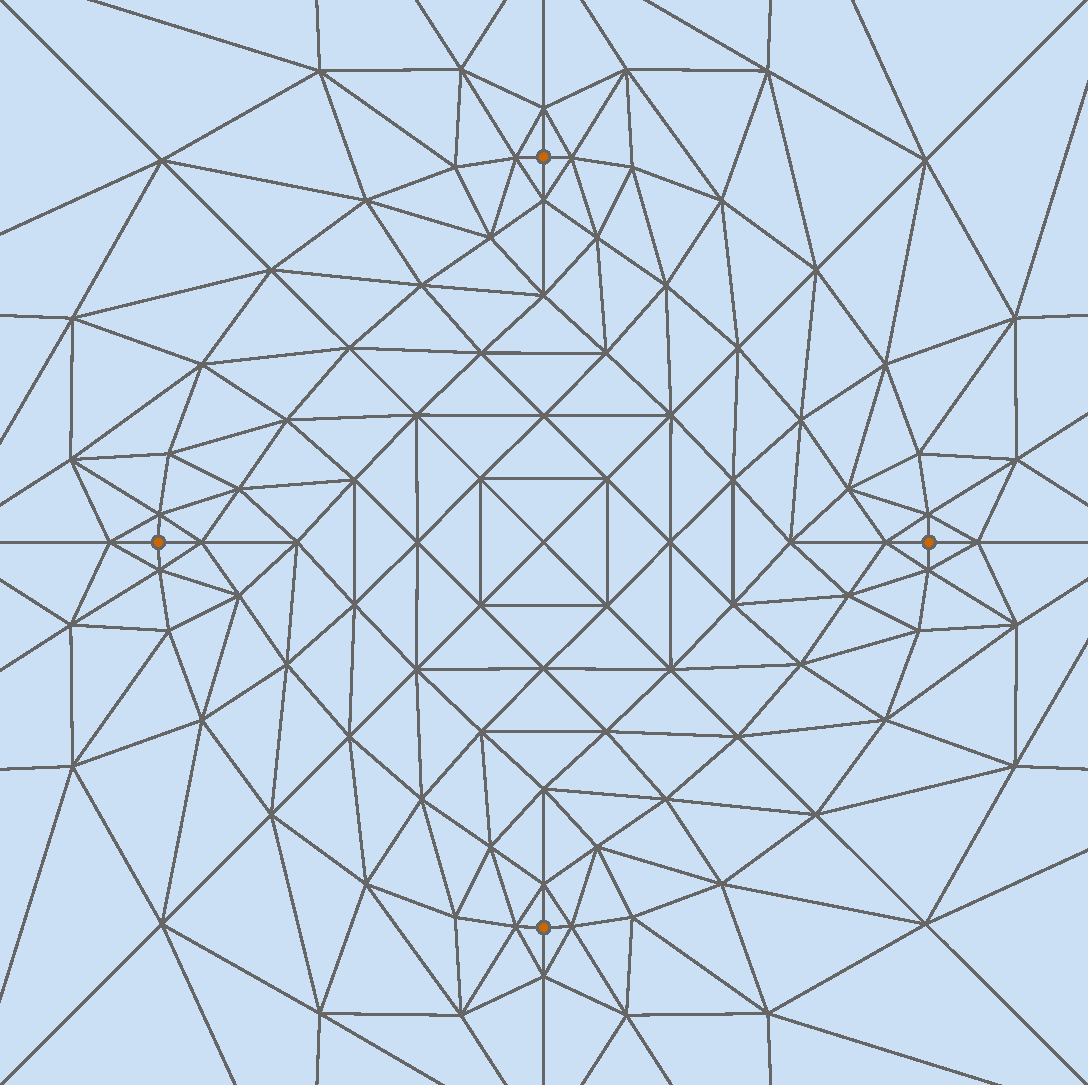
\includegraphics[height=4.7cm]{elliptic_square_uniform/square_uniform_fine_image.pdf}
}
\setstretch{0.8}{\scriptsize\tt data/elliptic\_square\_uniform/square\_branched.xml}
\caption{
Map from the flat torus $\tau=i$ to $\Chat$. 
Left: Subdivided lattice of the torus. 
Right: Two-sheeted image of the conformal map to $\Chat$, both sheets coincide due to the regular subdivision. 
Red point correspond to the four branch points under stereographic projection.
}
\label{fig:square_elliptic} 
\end{figure}

We can also create the inverse construction. 
Instead of starting at a branched configuration in $\hat \C$ we take the elliptic lattice in $\C$ and subdivide regularly.
We prescribe angle sums of $4\pi$ at the branch points of the map, i.e., the vertex of the lattice, the mid-points of edges, and the center of the fundamental parallelogram.
Construct the mapping to the sphere analogously to the construction used for unbranched spheres described in Section~\ref{sec:spheres_euclidean}.
Use one of the branch points to act the role of the point at infinity.
Then proceed with the finite part of the branched cover.
Insert the branch point at the north pole after stereographic projection to arrive at the solution.

In this spirit we calculate examples for the curves $\mu^2=\lambda(\lambda^3-1)$ and $\mu^2=\lambda^4-1$, i.e., the lattices $\tau=\frac{1}{2}+\frac{\sqrt 3}{2}i$ and $\tau=i$, see Figures~\ref{fig:wente_elliptic} and~\ref{fig:square_elliptic}.

\subsection{Regular triangulations on the sphere}
\label{sec:spherical_triangulations}

To create a reasonably regular triangulation with vertices on the sphere we minimize the following energy on a given set of initial points on the sphere while fixing the branch points. 
A good start is to choose points uniformly distributed on the sphere. 
To achieve this we choose $x$, $y$, and $z$ to be normally distributed and project the resulting vectors to the sphere~\cite{Muller1959}. 
The functional and its gradient that we minimize is
\begin{eqnarray*}
E &=& n^2\sum_{v\in V}\left( \left<v,v\right> - 1\right)^2 + \sum_{v\in V}\sum_{\substack{w\in V\\w\neq v}} \frac{1}{\left<w-v, w-v\right>}\\ 
\frac{\partial E}{\partial v} &=& 4n^2\left<v,v\right>v + 4\sum_{\substack{w\in V\\w\neq v}}\frac{w-v}{\left<w-v,w-v\right>^2}.
\end{eqnarray*}
$\left<.,.\right>$ is the standard euclidean scalar product. There is however no guarantee that the points of the minimizer will lie on the sphere and so we project after optimization.

\subsection{Discrete elliptic curves - numerical convergence}
\label{sec:numerical_convergence}

An algebraic curve of genus $g=1$ is called an elliptic curve. We model discrete elliptic curves as described in Section~\ref{sec:discrete_algebraic_curves}.

The goal of this section is to provide insights into the convergence behavior of discrete uniformization as presented above. In particular we look into the convergence of period matrices as the number of points that approximate a given Riemann surface increases. For genus one algebraic curves we can calculate period matrices explicitly using the invariants $\{g_2,g_3\}$ of the elliptic surface. Let $\lambda_1,\lambda_2,\lambda_3,\lambda_4\in\C$ be the branch points of the curve such that $\lambda_1+\lambda_2+\lambda_3=0$ and $\lambda_4=\infty$. Then the curve is given as
\begin{eqnarray*}
\mu^2&=&4(z-\lambda_1)(z-\lambda_2)(z-\lambda_3)\\
&=&4z^3+4(\lambda_1\lambda_2+\lambda_2\lambda_3+\lambda_3\lambda_1)z - 4\lambda_1\lambda_2\lambda_3\\
&=&4z^3-g_2z-g_3.
\end{eqnarray*}
The period matrix $[\tau]$, also called the modulus of the curve, can be calculated using the periods of the elliptic lattice $\{\omega_1,\omega_3\}$ such that $\tau = \frac{\omega_2}{\omega_1}$. These can be calculated from the invariants $\{g_2,g_3\}$, e.g., using {\sc Mathematica}s build-in function {\tt WeierstrassHalfPeriods[$\{g_2,g_3\}$]}~\cite{WeierstrassHalfPeriods_website}.

Let $\lambda_1, \lambda_2, \lambda_3, \lambda_4 \in \C$ be the branch points of an elliptic curve $C$. We create a discrete version of the curve by choosing $n$ points $p_1,\ldots,p_n$ equally distributed on $\S^2$. The triangulation for one sheet of the discrete curve is the convex hull of $\{\lambda_1,\ldots,\lambda_4,p_1,\ldots, p_4\}$. Choose non-intersecting edge-paths connecting the pairs $(\lambda_1,\lambda_2)$ and $(\lambda_3,\lambda_4)$. To create a doubly covered sphere we glue a second copy of the triangulated sphere transversely along corresponding paths, see Section~\ref{sec:discrete_algebraic_curves}.

After discrete uniformization we calculate $\hat \tau$. We normalize $\tau$ and $\hat \tau$ such that $|\tau|>1$ and $|\re(\tau)| < \frac{1}{2}$. We can now compare the modulus $\tau$ of the smooth structure with the number $\hat \tau$ derived from the discrete uniformization of a triangulation with the same branch points. The discretization error is defined as $|\tau-\hat \tau|$.

\subsubsection{Subdivided icosahedron}

\begin{figure}
\centering
\resizebox{\textwidth}{!}{
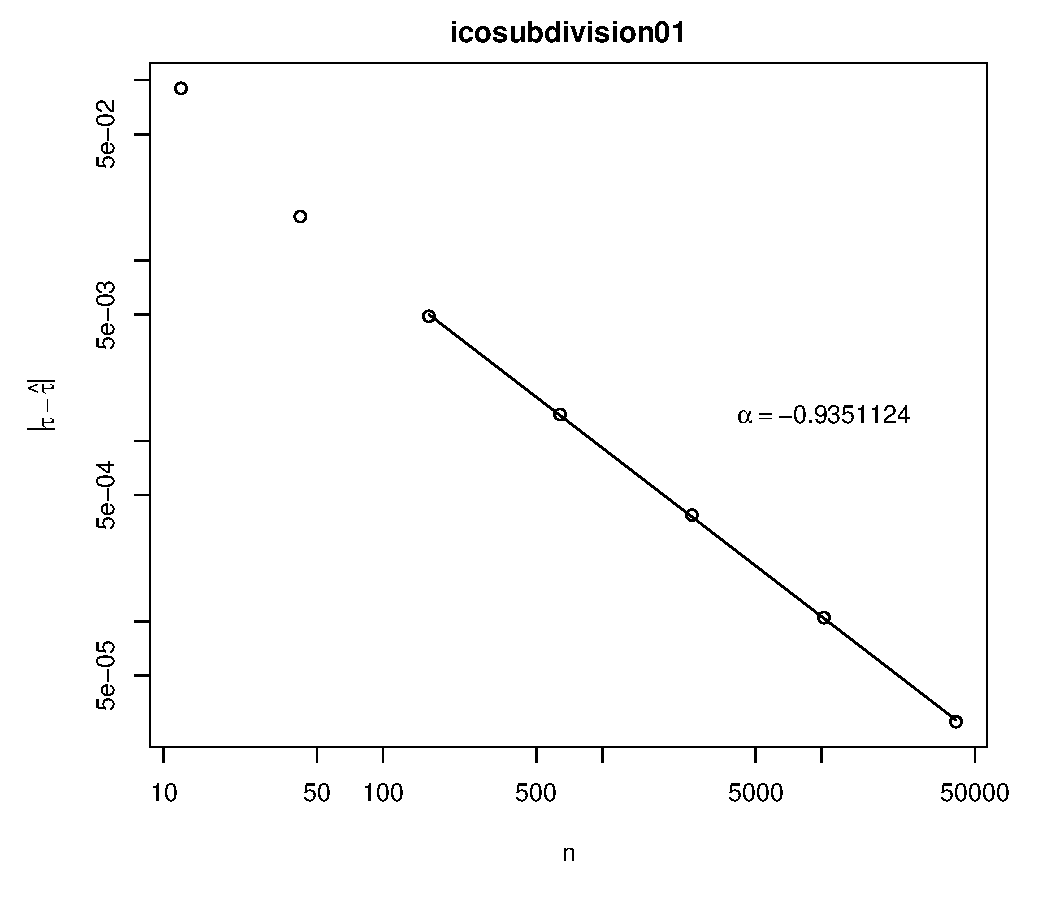
\includegraphics[width=0.35\textwidth]{convergence/icosubdivision01.pdf}\hfill
\includegraphics[width=0.32\textwidth]{convergence/icosubdivision01_example01.pdf}
}
\setstretch{0.8}
{\scriptsize\tt data/convergence/subdivision/icosubdivision01.dat}\\
{\scriptsize\tt data/convergence/subdivision/data/icosubdivision01.xml}
\caption{Numerical convergence for seven subdivision steps of an icosahedron.
Four vertices of the base icosahedron serve as branch points of a torus.
Vertices are projected to the unit sphere after subdivision.
The error $|\tau - \hat\tau|$ plotted against the number of vertices of one sheet of the double cover (left).
The linear regression of logarithmic data has a slope of $\alpha\approx-0.88$.
Universal cover of step three of the series (right).
}
\label{fig:convergence_subdivision}
\end{figure}

In this experiment we start with a regular icosahedron and choose $\lambda_1,\ldots,\lambda_4$ to be four of the vertices. The remaining points act the role of $p_1,\ldots,p_n$ and we construct the discrete elliptic curve as described above. To study the dependence of $|\tau-\hat \tau|$ on the number of points we increase $n$ by subdivision and subsequent projection onto $\mathbb S^2$. Every triangle is split into four. New vertices are inserted in the middle of each edge then we project onto the unit sphere. By this procedure we yield exponential growth of vertex number while at the same time the shape of the triangles stays almost regular.

Figure~\ref{fig:convergence_subdivision} shows the result of this convergence experiment. The error $|\tau-\hat \tau|$ depends exponentially on the number of points
\[|\tau-\hat \tau|=\mathcal O (n^\alpha)\]
with $\alpha \approx -0.88$.

\subsubsection{Triangle quality}

\begin{figure}
\centering
\includegraphics[width=\textwidth]{convergence/quality_rand_points01_maxmultiratio_2.pdf}
\setstretch{0.0}{\scriptsize\tt data/convergence/numberofpoints/quality\_rand\_points01.dat}
\caption{Plotting the error $|\tau - \hat\tau|$ against the number of vertices for triangulations with varying quality (left). Requiring a certain level of quality reveals a clear convergence slope of $\alpha\approx -0.63$ (right).}
\label{fig:convergence_quality}
\end{figure}

In the second convergence experiment we choose $p_1,\ldots,p_n\in \mathbb S^2$ randomly. 
We want to analyze how the quality of the triangulation affects the convergence behavior. 
We define quanities that measure the regularity of the triangulation based on length cross-ratios given at edges or length multi-ratios given at faces of the triangulation
\begin{eqnarray*}
	Q_{\lcr}(e) &\vcentcolon=& \frac{1}{2}\left(\lcr(e) + \frac{1}{\lcr(e)}\right) - 1\label{eq:quality_lcr}\\
	Q_{\lmr}(f) &\vcentcolon=& \frac{1}{2}\left(\lmr(f) + \frac{1}{\lmr(f)}\right) - 1\label{eq:quality_lmr}.
\end{eqnarray*}
Here $\lcr$ is the length cross-ratio of an edge. 
$\lmr$ is the length multi-ratio defined on faces as $\lmr(f)=\prod_{e \in f}\lcr(e)$.
To achieve a certain span of qualities of meshes me optimize random meshes with the procedure described in Section~\ref{sec:spherical_triangulations}.

Figure~\ref{fig:convergence_quality} (left) shows a plot of $2600$ samples ranging from $n=20$ to $n=1500$. 
No clear convergence behavior is visible. 
Plotting only samples with a certain mesh quality as defined by the quality measures above reveals a linear upper bound for the error $|\tau-\hat \tau|$. 
For the plot in Figure~\ref{fig:convergence_quality} (right) we selected only samples with $\max_e \{Q_{\lmr}(e)\} < 0.3$. 
Similar results can be obtained using the quality measures $\max_e \{Q_{\lcr}(e)\} < x$ or $\mean_e \{Q_{\lcr}(e)\} < x$.

The results from these two experiments assert that there is a exponential dependence of the discretization error on the number of points if a certain quality of the mesh is met. 
Tests with other subdivision configurations suggest that the constant $\alpha$ is not universal.

\section{Uniformization of surfaces of higher genus}
\label{sec:higher_genus}

\begin{figure}
\centering
\resizebox{\textwidth}{!}{
\includegraphics[height=10cm]{genus3/genus3.pdf}
\includegraphics[height=10cm]{genus3/canonical_mesh.pdf}
\includegraphics[height=10cm]{genus3/canonical_cover.pdf}
}
\setstretch{0.5}{\scriptsize\tt data/genus3/data.xml}
\caption{Discrete uniformization of an embedded triangulated surface of genus $3$. Fundamental polygon with mesh and group generators (middle). Fundamental polygon normalized to canonical form. Universal cover (right).}
\label{fig:embedded_genus_3}
\end{figure}

%\begin{figure}
%\centering
%\resizebox{0.8\textwidth}{!}{
%\includegraphics[height=10cm]{genus5/genus5.pdf}
%\includegraphics[height=10cm]{genus5/fundamental.pdf}
%}\\
%\setstretch{0.8}{\scriptsize\tt data/genus5/data.xml}
%\caption{An embedded triangulated surface of genus $5$ (left). Discrete uniformization and fundamental polygon with  group generators in the Poincar\'e disk (right).}
%\label{fig:embedded_genus_5}
%\end{figure}

In this section we describe how to calculate uniformizations of cyclic polyhedral surfaces of higher $g>1$ genus. 
In particular we show how to construct the corresponding Fuchsian groups and fundamental domains in Section~\ref{sec:fundamental_domains}.
We revisit surfaces given by Schottky data in Section~\ref{sec:schottky} for genus $g>1$, see also Section~\ref{sec:tori_schottky} for Schottky uniformizations of tori.
Finally, in Section~\ref{sec:hyperbolic_circle_domain} we construct hyperbolic circle domains analogously to the constructions presented in Section~\ref{sec:circle_domains} for topological spheres or disks.

\subsection{Notation}

Let $R$ be a Riemann surface of genus $g>1$. 
Then $R$ has a representation as the quotient of the hyperbolic plane modulo a discrete group of hyperbolic isometries $G$
\begin{equation}
R=\mathbb{H} / G.
\end{equation}
Typically the group $G$ is presented a set of generating elements $A,B,C,D,\ldots$ of hyperbolic isometries together with a relation 
\begin{equation}
G=\left<A,B,C,D,\ldots\mid P(A,B,C,D,\ldots)=1\right>
\end{equation}
where $P$ is a product of elements and inverse elements of $G$. 
$G$ is called a Fuchsian group if it contains only hyperbolic elements.
In this section we denote the inverse elements of an element $A\in G$ as 
\begin{equation}
A'\vcentcolon=A^{-1}\in G.
\end{equation}
A fundamental domain of $G$ is a simply connected region $D$ of the hyperbolic plane such that $D$ tiles hyperbolic space under the group action of $G$.
A fundamental polygon of $G$ is a fundamental domain with polygonal boundary, i.e., the boundary consists of geodesic edges.
Each edge $a$ has a partner edge $a'$ and a corresponding element $A\in G$ such that 
\begin{equation}
A\cdot a=a'.
\end{equation}
That means an edge $a$ is mapped to $a'$ by the isometry $A$. Conversely we have $A'\cdot a'=a$.
We denote the ordering of edges in a fundamental polygons in a counter-clockwise fashion. 
A polygon $abcda'b'c'd'$ together with the corresponding group elements $A$, $B$, $C$, and $D$ that tile the hyperbolic plane gives rise to a Fuchsian group with relation $AB'CD'A'BC'D=1$.

\subsection{Computation of fundamental domains and Fuchsian groups}
\label{sec:fundamental_domains}

\begin{figure}
\centering
\resizebox{0.8\textwidth}{!}{
\includegraphics[height=3cm]{algorithm/step1_boundary.pdf}
\includegraphics[height=3cm]{algorithm/step2.pdf}
}\\
\resizebox{0.8\textwidth}{!}{
\includegraphics[height=3cm]{algorithm/step3.pdf}
\includegraphics[height=3cm]{algorithm/contract_combined.pdf}
}\\
\resizebox{0.8\textwidth}{!}{
\includegraphics[height=3cm]{algorithm/step5.pdf}
\includegraphics[height=3cm]{algorithm/step5_5.pdf}
}
\setstretch{0.0}{\scriptsize\tt data/algorithm/data.xml}
\caption{
Creating a fundamental polygon of a hyperelliptic surface:
Realizing a hyperbolic metric of a discrete surface (upper-left) creates a fundamental region with polygonal boundary.
Straighten the edges between vertices of the cut-graph (red points) creates a polygon with geodesic edges (upper-right and middle-left).
Cut-and-paste operations lead to a fundamental polygon with only one vertex and opposite sides identified, all vertices are equivalent under the group action (middle-right).
We normalize the group such that the intersection of the axes is the origin (bottom).
}
\label{fig:fundamental_polygon_algorithm}
\end{figure}

Let $R$ be a Riemann surface and let $\Sigma=(V_{\Sigma}, E_{\Sigma}, F_{\Sigma})$ be a discretization of $R$. 
Let $\lcr :E\to \R_{>0}$ be the euclidean discrete conformal structure of $\Sigma$ and $\ell:E\to \R_{>0}$ a metric realization. 
Let $(u, \lambda):V\times E_1\to \R^{\#V}\times\R^{\# E_1}$ be the minimizer of the hyperbolic functional and of the hyperbolic version of Problem~\ref{prob:total_angles}.
Then 
\begin{eqnarray}
\tilde \ell:E &\to& \R_{>0}\\
{\it ij}&\mapsto& 2\arsinh\left(e^{\frac{1}{2}(u_i+u_j)}\ell_{\it ij}\right)
\end{eqnarray}
is the unique hyperbolic metric without cone singularities that is by definition conformally equivalent to~$\ell$, see Section~\ref{sec:discr-conf-equiv}.

Following the combinatorics of $\Sigma$ and the new metric $\tilde \ell$ we create a simply-connected realization by breadth-first enumeration of the triangles of $T$. 
As a different approach one could use a shortest-path scheme as described by Erickson and Har-Peled~\cite{EricksonH02} and cut the surface open to form a simply connected domain.  
The resulting domain has boundary edges and vertices. 
Each boundary edge is identified with a unique partner. 
Each boundary vertex is identified with one or more other vertices. 
On the surface the boundary of the domain corresponds to a connected system of loops around surface handles, see, e.g., Figure~\ref{fig:embedded_genus_3} left.

In the first step we create a simplified domain by connecting vertices that are identified with more than two copies by geodesic arcs, see Figure~\ref{fig:fundamental_polygon_algorithm} (top-right and middle-left). 
Again a geodesic boundary arc is identified with a unique copy. 
This identification gives rise to a group of isometries $G$ as identified arcs have the same length. 
$G$ is a Fuchsian group of the first kind. 
The domain bounded by geodesic arcs is a fundamental domain of $G$.

In addition to breadth first layout we can also predefine the system of loops on the surface to prescribe the combinatorics of the fundamental domain and its identifications. 
This is however not always possible due to the combinatorics of the triangle mesh, i.e., a small valence at the base point of the loops forces the fundamental polygon to have more than one vertex. 
In such a situation we proceed by reducing the domain by edge contraction operations to arrive at a fundamental domain with a single identified vertex:

The algorithm to reduce a given fundamental polygon to a polygon with only one identified vertex is as follows. 
Select a vertex $v_0$ to be the base vertex of the polygon. 
Select an edge between $v_0$ and another vertex $v_1$. 
In the hyperbolic plane move $v_1$ onto $v_0$ by moving all copies of $v_0$ to the corresponding copies of $v_1$, possibly outside of the domain. 
Move adjacent geodesic arcs correspondingly, see Figure~\ref{fig:fundamental_polygon_algorithm} (middle-right). 
In the new domain $v_1$ is not a vertex anymore. 
Proceed until the domain has only one vertex. 
This process can also be seen as a sequence of cut-and-paste operations reducing the number of vertices $v\neq v_0$ one by one. 
A proof that this leads to a valid fundamental domain can be found in the book "Compact Riemann Surfaces" by Jost~\cite[p. 48]{Jost2007}.

It can be tedious to find a system of loops on a surface that lead to a specific order of sides in the fundamental polygon. 
We give algorithms that transform a given fundamental polygon and the corresponding group presentation to canonical form, i.e., the order of polygon sides is $aba'b'cdc'd'\cdots$. 
Here the side $a$ is identified with side $a'$. 
Additionally we give an algorithm that transforms the domain to opposite identification form, i.e., $abcd\cdots a'b'c'd'\cdots$.

During all transformations of the polygon and the group presentation we like to minimize the number of group element products. 
This is due to numerical reasons. 
Hyperbolic motions tend to accumulate numerical errors quite fast when building products~\cite{Floyd2002}.

\subsubsection*{Canonical Fundamental Domain.}

\begin{figure}
\centering
\resizebox{\textwidth}{!}{
\includegraphics[width=5cm]{algorithm/canonical_step0_labels.pdf}
\includegraphics[width=5cm]{algorithm/canonical_step1_labels.pdf}
\includegraphics[width=5cm]{algorithm/canonical_step2_labels.pdf}
}
\caption{Motions to transform a given fundamental domain into canonical form. The shaded area is the current fundamental polygon. Step~$1$: Choose the linked pair $a$, $b$. Cut at $c$ and $b$ and identify via $B$ to put side $a$ next to side $b$. Choose linked pair $e$, $f$. Cut between $e'$ and $d'$ and identify via $E'$ to put side $e'$ next to $f'$. The remaining handle $cdc'd'$ is already in place and we arrive at canonical form $aba'b'cdc'd'efe'f'$.}
\label{fig:canonical_algorithm}
\end{figure}

We start with a fundamental polygon with a single vertex as explained above. 
Then choose sides $a$ and $b$ such that the order in the polygon is $a\cdots b \cdots a' \cdots b' \cdots$. 
We perform a cut-and-paste operation such that sides $a$ and $b$ are next to each other after transformation, see Figure~\ref{fig:cut-and-paste-canonical}. 
In order to minimize the number of products we choose $a$ and $b$ such the number of sides in between $a$, $b$, $a'$, and $b'$ is minimal. 
We proceed cutting as described before to bring $b$ next to $a'$ and analogously $a'$ next to $b'$. 
We end up with a new polygon and the order $aba'b'\cdots$. 
Repeat this algorithm for the rest of the sides to arrive at canonical form. 
Again a proof can be found, e.g., in the book by Jost~\cite[p. 51]{Jost2007}.

The number of products built during the transformation of a linked pair $a$, $b$ depends on the number of polygon sides between $a$, $b$, $a'$, and $b'$. 
Let $C$ be the number of sides between $a$ and $b$. Let $D$ and $E$ be the number of sides between $b$, $a'$, and $b'$ respectively. 
Then the total number of products in this transformation is $6C+4D+2E$. 
In step $1$, connecting $a$ and $b$, we can perform the cut-and-past operation using transformation $b$ and a cut between the end of $a$ and the end of $b$ in counter-clockwise order. 
This moves the intermediate sides between $a$ and $b$ out of the way for the next $2$ steps. 
By this we have a total number of products $2C+4D+2E$. 
We use a greedy implementation that chooses the smallest number of products in each step to select $a$ and $b$.
Alternatively one could enumerate the transformation tree and choose the cheapest path of all transformation sequences.

\begin{figure}
\centering
\resizebox{0.8\textwidth}{!}{
\includegraphics[width=5cm]{keen/canonical01_labels.pdf}
\includegraphics[width=5cm]{keen/keen01_labels.pdf}
}
\caption{
The algorithm of Linda Keen to construct strictly convex fundamental polygons. 
Start with a given canonical fundamental polygon $aba'b'cdc'd'$ with a corresponding relation $ABA'B'CDC'D'=1$ (left). 
For convenience labels are chosen such that both coincide. 
We choose the intersection $p_0$ of the axes of transformations $A$ and $B$ as base point for the new domain. 
The new vertices of the fundamental domain are calculated as $p_1=p_0\cdot B'A'$, $p_2=p_0\cdot A'$, $p_3=p_0\cdot B'$, and $p_4=p_0\cdot A'B'$. 
The vertices at the generators $C$ and $D$ are calculated from $p_4$.
}
\label{fig:keen_polygon}
\end{figure}

By this procedure we get a canonically identified fundamental polygon. 
This polygon may be non-convex. Following the approach described by Linda Keen~\cite{keen1966} we can transform this domain into a strictly convex fundamental polygon by selection of a different base point for the same group of transformations. Let
\begin{equation}
G=\left<A,B,C,D,\ldots\in \mathit{PSL}(2,\mathbb R)\mid ABA'B'CDC'D'\ldots=1\right>
\end{equation}
be a canonically presented group and $aba'b'cdc'd'\ldots$ be a corresponding fundamental polygon, see Figure~\ref{fig:keen_polygon} (left). 
Then the axes of the generators $A$ and $B$ intersect in a point $p_0$. 
Choosing $p_0$ as the base point of a new fundamental polygon renders it convex and uniquely defined for the given group and presentation. 
See Figure~\ref{fig:keen_polygon} for a genus $2$ instance of this algorithm.

\begin{figure}
\centering
\resizebox{0.4\textwidth}{!} {
\input{data/algorithm/cutCanonical.pdf_t}
}
\caption{Cut-and-paste: Cut from the start of $a$ to the start of side $b$. Glue the piece along $a'$ using transformation $A$ that moves side $a$ to $'a$. Intermediate sides $c_1,\ldots,c_n$ between $a$ and $b$ are transformed accordingly and group elements transform as $\hat{C_i}=A'C_i$. Their inverses $C_i'$ become $\hat{C_i}'=C_i'A$}
\label{fig:cut-and-paste-canonical}
\end{figure}

\subsubsection*{Opposite Sides Fundamental Domain.}

\begin{figure}
\resizebox{\textwidth}{!}{
\includegraphics[width=5cm]{algorithm/opposite_step0_labels_start.pdf}
\includegraphics[width=5cm]{algorithm/opposite_step0_labels.pdf}
\includegraphics[width=5cm]{algorithm/opposite_step1_labels.pdf}
}
\resizebox{0.666666\textwidth}{!}{
\includegraphics[width=5cm]{algorithm/opposite_step2_labels.pdf}
\includegraphics[width=5cm]{algorithm/opposite_step3_labels.pdf}
}
\caption{Algorithm example: Start with group relation $ABCDC' EFA'E'D'F'B' = 1$. Step~$1$: Cut from the start of $d'$ to the end of $c'$ and identify via $C'$ to move $C'$ in front of $D'$. The resulting relation is clustered such that the elements of the first half form the inverses of the second half: $ABCDEFA'E'C'D'F'B' = 1$. We now sort elements $A,\ldots,B$ to match the order of $A',\ldots,F'$ or vice versa. Step~$2$: Cut at $a'$ and $b$ and identify via $B$ to move $B$ in front of $A'$. We get relation $ACDEFBA'E'C'D'F'B' = 1$. Step~$3$: Cut between $d'$ and $e$ and identify via $E$ to move $E$ in front of $C$. We get $AECDFBA'E'C'D'F'B' = 1$ as the final relation and a fundamental polygon with oppositely identified sides.}
\label{fig:opposite_algorithm}
\end{figure}

\begin{figure}
\centering
\resizebox{0.3\textwidth}{!} {
\input{data/algorithm/moveElement.pdf_t}
}
\caption{Move element $A$ in front of $B$ in a relation that moves counter-clockwise around the base vertex. Choose the upper cut (dashed lines) and paste via transformation $A'$ moving side $a'$ to $a$. Or cut at the lower one and paste via transformation $A$.}
\label{fig:cut-and-paste-motion}
\end{figure}

A fundamental polygon identified by opposite sides has a side ordering $abcd\cdots a'b'c'd'\cdots$. A corresponding relation of the group of hyperbolic translations is $AB'CD'\cdots=1$ given that a transformation $X$ maps side $x$ to $x'$.

We give two algorithms to transform a given fundamental domain into an opposite sides domain.
For the first algorithm we show that it terminates and yields the correct result. However we cannot control the number of products used during the transformation. The second algorithm is heuristic and minimizes the number of products. It has proven to terminate for all of our examples.

We use the canonical form of fundamental polygons as an intermediate step in the process of transforming a given fundamental domain into opposite sided form. As shown above we can transform any domain into canonical form. In particular we can transform an abstract oppositely identified polygon into canonical form using the algorithm from above. All of the steps conducted during this transformation can be undone. We get a sequence of cut-and-paste operations transforming a canonical fundamental polygon into opposite sides form. Combining the sequence that transforms a general fundamental polygon into canonical form with the transform that creates the opposite form from the canonical one we get required sequence on transformations on any given domain.

This version of the algorithm is not optimal with respect to the number of products used in the sequence of transformations. In particular if the input polygon is close to opposite sides form already, the algorithm destroys this structure first and rebuilds it from the canonical form.

In all examples we therefor use a different heuristic algorithm. We transform a given fundamental polygon and group presentation to opposite sides form using the following sequence of transformations. Refer to Figure~\ref{fig:opposite_algorithm} for an instance of this algorithm:

For a given fundamental polygon and the ordering of its sides, we can reconstruct the relation of the group by moving around the base vertex on the surface. That means if we start with transformation $A$ moving side $a$ to $a'$ the next element in the relation belongs to the side next to $a'$ in counter-clockwise order. We proceed until we get back to element $A$. Note that we could have chosen clockwise orientation, but for drawing pictures we stick to counter-clockwise.

For an oppositely identified fundamental polygon (and for canonically identified polygons as well) the order of transformations in the relation has the same structure as the sides of the polygon (possibly after renaming of sides). For example the group relation corresponding to a polygon $ab'cd'a'bc'd$ is $ABCDA'B'C'D'=1$.

For the order of group elements in the relation we give cut-and-paste sequences that move single elements to different locations in the relation leaving all other elements in place. Using these transformations we normalize the polygon as follows.

\begin{compactitem}
\item[1] Find largest sequence of different (excluding inverse) generators in the relation.
\item[2] Move missing elements into the sequence such that it forms a basis for the group.
\item[3] Sort elements in the sequence to match the order of the corresponding inverse elements.
\end{compactitem}

Let the order of sides in the polygon be $a' \cdots b \cdots a \cdots$. The corresponding cut-and-paste operation that moves the group element $A$ in front of $B$ is one of

\begin{compactitem}
\item Cut from the end of $a$ to the start of $b$ and glue using $A$.
\item Cut from the start of $a'$ to the start of $b$ and glue via $A'$.
\end{compactitem}

Choose the one with the lowest number of products, see Figure~\ref{fig:cut-and-paste-motion}. If the order of sides in the polygon is $a' \cdots a \cdots b \cdots$ we can however not perform the operation, the resulting domain would be disconnected. We therefor define the cost for such an operation as infinite. In step 2 we minimize over all possible transformations that move a selected element into the sequence. We do not show here that the cost is always a finite during the algorithm and call this algorithm heuristic due to this fact. Depending on the sort algorithm we use in step 3 we have the freedom to choose between the motion of the inverse elements or their partners. In our examples this gives enough freedom to create all oppositely identified fundamental domains. See Figure~\ref{fig:opposite_algorithm} for an example of this algorithm.


\subsection{From Schottky to Fuchsian uniformization}
\label{sec:schottky}

\begin{figure}
\centering
\resizebox{\textwidth}{!}{
\reflectbox{\includegraphics[width=10cm, angle=90]{schottky_g3/genus3_image2.pdf}}
\includegraphics[width=10cm]{schottky_g3/genus3_domain2.pdf}
}
\setstretch{0.0}{\scriptsize\tt data/schottky\_g3/schottky.xml} 
\caption{
Left: Discrete version of a Riemann surface of genus $3$ given by Schottky data.
Circles with the same color are identified.
The Schottky group elements that map the blue and green circles onto each other map the exterior of the source circle onto the interior of the image circle and vice-versa.
The map corresponding to the purple circle is defined to map the interior of the outer circle to the interior of the inner circle. Stereographically projected image, the randomly chosen extra points of the triangulation are chosen such that the triangulation is close to regular where possible.
\\
Right: Fuchsian uniformization and universal cover in the Poicar\'e model of the hyperbolic plane. The boundary of the fundamental domain consists of  the Schottky circles and short paths connecting them (grey edges).
}
\label{fig:schottky_g3}
\end{figure}

We have treated Schottky data in the case of tori in Section~\ref{sec:tori_schottky}.
The general construction for surfaces with genus greater that one is parallel to the construction in the torus case.
For a given conformal structure, i.e. the length cross-ratios on edges, we find a critical point of the hyperbolic functional.
We visualize the Fuchsian uniformization in the Poicar\'{e} model and highlight the images of the circles, Figure~\ref{fig:schottky_g3}.
Additionally to the vertices on the circles we choose random points in the fundamental domain on $\Chat$ such that the triangulation is close to regular.
We optimize the vertex location using the process described in Section~\ref{sec:spherical_triangulations}.
Vertices that land in the interior of the circles are discarded.

\subsection{Hyperbolic uniformization with circular boundaries}
\label{sec:hyperbolic_circle_domain}

\begin{figure}
\centering
\resizebox{\textwidth}{!}{
\raisebox{0.75cm}{
\includegraphics[height=3.5cm]{circle_domain_hyperbolic/brezel_three_holes_edges.pdf}
}
\includegraphics[height=5cm]{circle_domain_hyperbolic/brezel_three_holes_domain.pdf}
}
\setstretch{0.0}{\scriptsize\tt data/circle\_domain\_hyperbolic/brezel\_\{one,two,three\}\_holes.xml}
\caption{
Uniformization of a genus $2$ surface with three boundary components. 
The three holes are filled and triangulated (highlighted edges) to visualize the triangulation used during calculation, see Section~\ref{sec:circle_domains}.
}
\label{fig:hyperbolic_circle_domain}
\end{figure}

Let R be a Riemann surface with genus $g>1$ and $n$ boundary components.
There is a Fuchsian uniformization of $R$ that maps the boundary components onto circles. \todo{Find reference}
In the discrete setting we construct this uniformization using a similar approach as for euclidean circle domains.
Fill each of the boundary components with a face.
Treat the extra faces as if they were cyclic faces to begin with, i.e., the corresponding $\lambda$s in the auxiliary triangulation are variables of the variational principle.
The critical point of the hyperbolic functional is a hyperbolic flat metric with cyclic faces even at the extra faces.
Remove the extra faces to arrive at the fundamental domain with circular boundary components, see Figure~\ref{fig:hyperbolic_circle_domain}.


\section{Uniformization of hyperelliptic surfaces}
\label{sec:hyperelliptic}

A hyperelliptic surface is a Riemann surface of genus $g>1$ that has a realization as a 2-sheeted branched cover of $\Chat$.
Any Riemann surface of genus $2$ is hyperelliptic.
In this section we construct uniformizations of discrete versions of hyperelliptic Riemann surfaces.

We proof a characterization of hyperelliptic Riemann surfaces in terms of the geometry of the fundamental group. 
We construct fundamental domains specially designed to match the hyperelliptic structure of the surfaces, i.e., oppositely identified polygons with a branch point at the vertex.
These objects are the natural generalizations of the euclidean lattices in the elliptic case, see Section~\ref{sec:tori}.
We check this characterization with a specifically designed hyperelliptic surface of genus $3$.
In Section~\ref{sec:lawson_uniformization} we construct uniformizations of Lawson's minimal surface of genus $2$. We present different conformally equivalent realizations and the corresponding uniformizations together with fundamental domains.

In order to construct a discrete version of a hyperelliptic surfaces we first treat the case of hyperelliptic algebraic curves:
\begin{equation}
C=\left\{(\mu,\lambda)\in \C^2 \mid \mu^2=\prod_{i=1}^{2g+2}(\lambda - \lambda_i)\right\}
\end{equation}
with branch points $\lambda_1,\ldots,\lambda_{2g+2}\in \Chat$.
We always work with the conformally equivalent projection $(\mu, \lambda)\mapsto \lambda$ that defines a two-sheeted covering of $\Chat$ branched at $\lambda_1,\ldots,\lambda_{2g+2}$. 
As in the elliptic case, see Section~\ref{sec:discrete_algebraic_curves}, we construct a suitable triangulation and glue two copies of it along cuts connecting the vertices that act the role of the branch points.

\begin{figure} 
\centering
\resizebox{\textwidth}{!}{
\includegraphics[height=4.5cm]{hyperelliptic_g2/cover.pdf}
\includegraphics[height=4.5cm]{hyperelliptic_g3/cover_mesh.pdf}
\includegraphics[height=4.5cm]{hyperelliptic_g4/cover.pdf}
}
\setstretch{0.0}{\scriptsize\tt data/hyperelliptic\_\{g2,g3,g4\}/data.xml} 
\caption{
The hyperelliptic surfaces of Equation~\ref{eq:hyperelliptic_roots_unity} with genus 2, 3, and 4. 
The fundamental polygons can be chosen to be regular hyperbolic $4g$-gons. 
The triangulation of the surfaces is a subdivision of the convex hull of the branch points.
} 
\label{fig:roots_of_unity_curve} 
\end{figure}

We calculate the Fuchsian uniformizations of the curves
\begin{equation}
	\mu^2=\lambda\prod_{k=1}^{2g}\left(\lambda-e^{\frac{ik\pi}{g}}\right).\label{eq:hyperelliptic_roots_unity}
\end{equation}
Thus the corresponding $2$-sheeted cover of $\Chat$ exhibits branch points at the $(2g)$th roots of unity, at $0$, and at $\infty$. 
In this special case we can choose the fundamental domain to be a regular $4g$-sided hyperbolic polygon, see Figure~\ref{fig:roots_of_unity_curve}.

Note that the regular fundamental polygon is identified by opposite edges and the corresponding axes of the group elements meet in a common point.
The axis of a hyperbolic motion is the unique geodesic joining the two fixed points of the motion on the circle that represent the points at infinity.
This property is a characteristic property of hyperelliptic surfaces and investigated further in the next section.

\begin{figure} 
\centering
\resizebox{\textwidth}{!}{
\includegraphics[height=4.5cm]{branched_genus_2/mercator_texture.pdf}
\includegraphics[height=4.5cm]{branched_genus_2/image_mercator_closeup.pdf}
}
\setstretch{0.0}{\scriptsize\tt data/branched\_genus\_2/data.xml} 
\caption{
A genus $2$ surface mapped to a branched cover of $\Chat$. 
The surface exhibits an extrinsic conformal involution, the rotation about the horizontal axis of symmetry. 
Its fixed points correspond to the branch points of the corresponding hyperelliptic algebraic curve.
The involution corresponds to the hyperelliptic involution of the curve.  
Left: Surface and branch points with texture after Mercator projection using the purple
branch points as poles. 
Right: A closeup of the stereographic projection of one pair of red and blue branch points.
} 
\label{fig:genus2_branched} 
\end{figure}

As in the elliptic case we can invert this construction if we know the location of the branch points on the surface.
If the hyperelliptic involution of the surface is realizable as an extrinsic involution on an embedded surface we can easily select the branch points as the fix points of this transformation, see Figure~\ref{fig:genus2_branched}. 
Once the branch points are known we can proceed as described in Section~\ref{sec:discrete_algebraic_curves} to calculate a map from the surface to $\Chat$.

\subsection{Fundamental domains domains for hyperelliptic surfaces}
\label{sec:hyperelliptic_domain}

The images in Figure~\ref{fig:roots_of_unity_curve} suggest that we can find special fundamental domains for hyperelliptic surfaces, see also Figure~\ref{fig:fundamental_polygon_algorithm} (bottom) for a more irregular polygon. 
And indeed for every hyperelliptic Riemann surface we can find a basis of the uniformizing group such that the axes of the transformations meet in a common point.
The opposite the also true and we state the following

\begin{theorem}[Characterization of hyperelliptic surfaces]
\label{thm:hyperelliptic}
Let $R$ be a Riemann surface and let $G$ be its uniformizing Fuchsian group with generators $A_1,\ldots,A_{2g}$.
Then the following statements are equivalent:
\begin{compactitem}
\item $R$ is hyperelliptic.
\item There exist generators $A_1,\ldots,A_{2g}$ of $G$ whose axes meet in a common point.
\end{compactitem}
Further, we can choose a fundamental polygon with minimal number of sides and a single vertex such that the branch points of the corresponding hyperelliptic curve are located at the vertex, the intersection of the axes, and the mid points of the edges of the polygon.
\end{theorem}

\begin{proof}
This was first proved by Schmutz Schaller in a different fashion~\cite{schmutz1999, schmutz2000}.
Let $a_1,\ldots,a_{2g}$ be the axes of the transformations $A_1,\ldots,A_{2g}$ and let $x_0$ be their common point of intersection. 
Let $h$ be the hyperbolic rotation about $x_0$ by $180\degree$. $h$ is a hyperbolic isometry and $h^2=1$, i.e., $h$ is a holomorphic involution of $\H^2$ with fixed point $x_0$. 
We will show that $hGh^{-1}=hGh=G$. 
This renders $h$ a holomorphic involution on the surface $R=\H^2/G$.

Let $A_k$ be a generator of $G$ and let $\ell_k$ be the distance between $x_0$ and $A_kx_0$ denoted by $d(x_0,A_kx_0)$.
\begin{eqnarray}
d(x_0,hA_khx_0)&=&d(hx_0,hA_kx_0)\label{eq:hyper_dist_fixpoint}\\
&=&d(x_0,A_kx_0)\label{eq:hyper_dist_isometry}\\
&=&\ell_k.
\end{eqnarray}
Here we use that $x_0$ is a fixed point of $h$ (Equation~\ref{eq:hyper_dist_fixpoint}) and that $h$ is a hyperbolic isometry (Equation~\ref{eq:hyper_dist_isometry}). 
The axes $a_k$ of the generators $A_k$ are invariant under the transformation $h$ since its fixed point is contained in $a_k$.
Using the fact the $A_k$ is an isometry and applying the triangle inequality on the line $a_k$ we yield
\begin{eqnarray*}
d(A_kx_0,A_khA_khx_0)&=&d(A_kx_0,x_0)\pm d(x_0,A_khA_khx_0)\\
&=&\ell_k.
\end{eqnarray*}
This implies that $d(x_0,A_khA_khx_0)=0$ and $A_khA_khx_0=x_0$.
That means that $A_khA_kh$ is the identity on the axis $a_k$ thus it is the identity on $\H^2$. 
Now take any group element $B$ as the composition of generators $A_1,\dots,A_{2g}$. 
The conjugation $hBh$ is a group element of $G$ as the conjugation of each of the generators is.

Let now $R$ be any hyperelliptic Riemann surface. There is a holomorphic involution $h$ on $R$ with $2g + 2$ fixed points $x_1,\ldots,x_{2g+2}$. 
Let $\tilde x_1$ be a point in the universal cover corresponding to $x_0$ on the $R$. Let $\tilde x_3,\ldots,\tilde x_{2g+2}$ be the closest points in the universal cover corresponding to the other fixed points of $h$. Note that we leave out $x_2$ as we only need $2g$ cycles to define a basis of uniformizing group. 
The points $\tilde x_3,\ldots,\tilde x_{2g+2}$ are not unique but the following reasoning works for arbitrary choices.
In the universal cover $h$ corresponds to an involution $\tilde h$ with one fixed point, e.g., a hyperbolic rotation by $180\degree$ about $\tilde x_1$.
Consider the shortest geodesics $\tilde a_3,\ldots,\tilde a_{2g+2}$ connecting $\tilde x_1$ with $\tilde x_3,\ldots,\tilde x_{2g+2}$.
Then the curve $(a_i, h a_i)$ is a simple closed geodesic loop on $R$.
All curves $(a_i, h a_i)$ intersect uniquely at $x_1$. 
For a geodesic $(\tilde a_i, \tilde h \tilde a_i)$ define $\ell_i$ to be its lengths.
Define $A_i$ to be the hyperbolic motion with axis $(\tilde a_i, \tilde h \tilde a_i)$ and transport distance $\ell_i$.
Then $A_3,\ldots,A_{2g+2}$ form a basis of the uniformizing Fuchsian group.
By definition the axes of $A_3,\ldots,A_{2g+2}$ intersect in a common point.
\end{proof}

We now construct a symmetric fundamental domain for hyperelliptic surfaces.
As in the proof let $\tilde x_1$ be the fixed point of the rotation corresponding to the hyperelliptic involution of $R$ in the universal cover.
Pick the closest point $\tilde x_2$ in the universal cover corresponding to $x_2$ on $R$.
As before $\tilde x_2$ is not unique.
Construct a fundamental domain of the group by reflecting $\tilde x_2$ across the axes of the generators $A_i$ to obtain a fundamental polygon with $4g$ sides.
By construction the polygon is symmetric with respect to $\tilde h$. 
$\tilde h$ is an involution on the fundamental domain defined by the polygon.
An alternative algorithm to construct this polygon is given in Section~\ref{sec:fundamental_domains}.

\subsection{Hyperelliptic vs. non-hyperelliptic curves}
\label{sec:non-hyperelliptic}

\begin{figure}
\centering
\resizebox{!}{7cm}{
\rotatebox{90}{
\includegraphics[width=0.4\textwidth]{non-hyperelliptic/tetra_symmetric_hyperelliptic.pdf}
}
\rotatebox{90}{
\includegraphics[width=0.4\textwidth]{non-hyperelliptic/non-hyperelliptic-symmetric-with-closeup.pdf}
}
}
\setstretch{0.0}{\scriptsize\tt data/non-hyperelliptic/tetrahedron\_g3\_01\_symmetric.xml}
\caption{Hyperelliptic vs. non-hyperelliptic. In the hyperelliptic case axes of hyperbolic translations meet in a common point. The fundamental polygon is chosen symmetric with respect to the hyper elliptic involution (left). If the symmetry of the surface is broken the axes do not meet and no symmetric domain can be found (right).}
\label{fig:non-hyperelliptic}
\end{figure}

Consider the elliptic-hyperelliptic surface that is constructed as follows. Take two copies $\hat T$ and $\tilde T$ of the elliptic surface $y^2=x(x^3 - 1)$. Each of the copies is conformally equivalent to a torus with the modulus $\tau=\frac{1}{2}+\sin(\frac{\pi}{3})i$. Such a torus can be realized as the double cover of a generating regular tetrahedron branched at its four vertices.

On both copies of this torus pick four points $\hat\lambda_1,\ldots,\hat\lambda_4$ and $\tilde\lambda_1,\ldots,\tilde\lambda_4$ in the center of the faces of the tetrahedron belonging to one of the sheets of the elliptic surface. On $\hat T$ choose paths connecting the pairs $(\hat\lambda_1,\hat\lambda_2)$ and $(\hat\lambda_3,\hat\lambda_4)$. On $\tilde T$ choose corresponding paths. Cut $\hat T$ and $\tilde T$ along theses paths and glue corresponding sheets transversally. The resulting surface $T$ is a four sheeted cover of the tetrahedron with genus $g = 3$.

\begin{theorem}
$T$ is a hyperelliptic Riemann surface.
\end{theorem}

\begin{proof}
Let $e_1,\ldots,e_6$ be the edges of the generating regular tetrahedron. Consider the reflection $\sigma_i$ across a plane through the midpoint of edge $e_i$ containing the opposite edge of $e_i$.  Because of the symmetry of the tetrahedron $\sigma_i$ induces an anti-holomorphic involution on $T$. There are six involutions belonging to the edges of the tetrahedron. Let $e_i$ and $e_j$ be two opposite edges. Then $\sigma_i \circ \sigma_j$ is a holomorphic involution of $T$. Its eight fix points are the mid points of $e_i$ and $e_j$.
\end{proof}

Figure~\ref{fig:non-hyperelliptic} (left) shows a uniformization of $T$ with an oppositely identified fundamental polygon. The surface is hyperelliptic, thus the generators axes meet in a common point. Disturbing the symmetry a little, e.g., by moving all points of the surface by some random offset destroys the hyperellipticity of the surface, see Figure~\ref{fig:non-hyperelliptic} (right).

\subsection{Lawson's surface}
\label{sec:lawson_uniformization}

In this section we present the Fuchsian uniformization of the Riemann surface of Lawson's genus 2 minimal surface in $\mathbb{S}^3$ \cite{Law1970}.
We use three different conformally equivalent representations of the surface and compare the resulting uniformizations.
Namely a stereographically projected embedded version, see Figure~\ref{fig:lawson_embedding}.
The model has been provided by Konrad Polthier~\cite{polthier97}.
The conformally equivalent algebraic curve $\mu^2=\lambda^6-1$, see Figure~\ref{fig:lawson_curve}.
And a conformally equivalent square-tiled surface glued from six squares, see Figure~\ref{fig:lawson_squares}.
All data presented in this section is made available on the {\sc DGD Gallery} \cite{gallery-lawson-webpage}.

For each of the representations we choose suitable fundamental domains that allow for the comparison of the uniformization.

\subsubsection{Hyperelliptic curve.}
\label{sec:lawson_curve}

\begin{figure}
	\centering
	\resizebox{!}{6cm} {
	\includegraphics[height=10cm]{lawson_curve/curve_canonical_cuts2.pdf}
	\includegraphics[height=10cm]{lawson_curve/curve_canonical_uniformization.pdf}
	}
	\setstretch{0.0}{\scriptsize\tt data/lawson\_curve/curve\_canonical.xml}
	\resizebox{!}{6cm} {
	\includegraphics[height=10cm]{lawson_curve/curve_opposite_cuts.pdf}
	\includegraphics[height=10cm]{lawson_curve/curve_opposite_uniformization.pdf}
	}
	\setstretch{0.0}{\scriptsize\tt data/lawson\_curve/curve\_opposite.xml}
	\resizebox{!}{6cm} {
	\includegraphics[height=10cm]{lawson_curve/curve_cyclic_cuts.pdf}
	\includegraphics[height=10cm]{lawson_curve/curve_cyclic_triangulation_cover.pdf}
	}
	\setstretch{0.0}{\scriptsize\tt data/lawson\_curve/curve\_cyclic.xml}
	\caption{Uniformization of Lawson's surface represented as algebraic curve $\mu^2=\lambda^6-1$. Triangulated double cover of the sphere branched at the roots of unity (left) with boundary of fundamental domain and axes of generators. Fuchsian uniformization and fundamental domain (right). Canonical domain (top), opposite sides domain (middle), and cyclic identification (bottom).}
	\label{fig:lawson_curve}
\end{figure}

Lawson's surface is conformally equivalent to the algebraic curve $\mu^2=\lambda^6-1$.
We model the surface as a two-sheeted cover of $\hat \C$ as described in Section~\ref{sec:discrete_algebraic_curves}. $\lambda_1,\ldots,\lambda_6$ are the 6th roots of unity.
See Figure~\ref{fig:lawson_curve}.

\textit{Canonical domain:}
For the canonical fundamental domain we pick $0$ to be the vertex of the domain and proceed as described in Section~\ref{sec:fundamental_domains}.
The points $p_1,\ldots,p_n$ are chosen such that the triangulation is almost regular on the sphere.
The system of loops on the surface is chosen such that each loop starts at vertex $0$ runs around two branch points and returns, see the red curves in Figure~\ref{fig:lawson_curve}, top-left.

For the visualization we truncate the triangles of the universal cover to fill the fundamental domain only.
Figure~\ref{fig:lawson_curve} shows the triangulation on $\hat \C$ (left) and the universal cover (right).
Red curves are the boundary of the fundamental domain.
We show them also pulled back onto $\hat \C$. Blue curves are closed geodesic loops on the surface.
They are the axis of hyperbolic motions identifying pairs of fundamental edges in the hyperbolic plane.

The branch points are clearly visible as the valence of the triangulation is doubled at these vertices.
The blue geodesic loops connect two branch points each.

\textit{Opposites sides domain:}
The opposite sides domain (second row) is chosen as described in Section~\ref{sec:hyperelliptic_domain}.
All axes of hyperbolic motions intersect in a branch point of the curve.
Red and blue geodesic arcs are dual to each other.
For the example model we chose a coarse discretization of the underlying curve and truncate the triangulation to fit into the fundamental domain.

\textit{Cyclically identified domain:}
We call the fundamental domain in the bottom row a cyclically identified domain.
This domain is chosen such that is corresponds to the domain suited for the square-tiled surface as described below.
You can imagine this system of loops if you take the canonical system of loops meeting at $0$ (top row of the Figure) and deform the loops until they touch at $\infty$.
By this move we introduce two more vertices on the fundamental polygon, namely the two vertices corresponding to $\infty$ on the two-sheeted cover.
The triangulation of the example model is created by a subdivision process.
Starting from  a triangulation with vertices at $0$, $\infty$, at branch points, and the mid-points on the equator in between the branch points we subdivide using a linear 4-to-1 split followed by a projection to the sphere. Thus the boundary of the fundamental domain is contained in the edge set of the triangulation. For the visualization of the universal cover we cut along these edges to draw the triangulation, Figure~\ref{fig:lawson_curve}, bottom-right.

\subsubsection{Stereographic embedding.}

\begin{figure}
	\centering
	\resizebox{!}{6cm} {
	\includegraphics[height=10cm]{lawson_embedding/embedding_canonical_cuts.pdf}
	\includegraphics[height=10cm]{lawson_embedding/embedding_canonical_uniformization.pdf}
	}
	\setstretch{0.0}{\scriptsize\tt data/lawson\_embedding/embedding5k\_canonical.xml}
	\resizebox{!}{6cm} {
	\includegraphics[height=10cm]{lawson_embedding/embedding_opposite_cuts.pdf}
	\includegraphics[height=10cm]{lawson_embedding/embedding_opposite_uniformization.pdf}
	}
	\setstretch{0.0}{\scriptsize\tt data/lawson\_embedding/embedding5k\_opposite.xml}	
	\resizebox{!}{6.5cm} {
	\includegraphics[height=10cm]{lawson_embedding/embedding_cyclic_cuts.pdf}
	\includegraphics[height=10cm]{lawson_embedding/embedding_cyclic_triangulation_cover.pdf}
	}
	\setstretch{0.0}{\scriptsize\tt data/lawson\_embedding/embedding5k\_cyclic.xml}	
	\caption{Uniformization of a euclidean embedding of Lawson's surface. Triangulated embedding with fundamental domain boundary and generator axes (left). Fuchsian uniformization with universal cover and fundamental domain (right). Canonical domain (top), opposite sides domain (middle), and cyclic identification (bottom).}
	\label{fig:lawson_embedding}
\end{figure}

Figure~\ref{fig:lawson_embedding}, top row, shows the Fuchsian uniformization of the Lawson surface with a canonical fundamental domain, see also Section~\ref{sec:fundamental_domains}.

Our embedded model of the Lawson surface of genus 2 realizes its hyperelliptic involution as a rotational symmetry.
Its symmetry axis meets the surface in six points. These fix points of the hyperelliptic involution correspond to the branch points of the hyperelliptic algebraic curve as seen in the example above. We uniformize this model and choose fundamental domains corresponding to the domains chosen in Section~\ref{sec:lawson_curve}. By this procedure we can visually compare the surfaces and get evidence on conformal equivalence of the smooth surfaces.

For the canonical fundamental domain we have to find a point on the surface that corresponds to $0$ or $\infty$ on the algebraic curve. There are of course four candidates as $0$ and $\infty$ correspond to two points each on the curve. We choose this point manually such that the fundamental domain exhibits the two reflectional symmetries seen in the domain of the curve.

The fundamental domain where opposite sides are identified is chosen as described in Section~\ref{sec:hyperelliptic_domain}. The rotational symmetry of the surface corresponds to the hyperelliptic involution of the surface. Its fix points, i.e. the intersection of the axis of symmetry with the surface, correspond to the branch points of the hyperelliptic curve. Thus the vertex of the fundamental polygon has to be a point on the symmetry axis of the surface. We choose one of the six points and proceed as explained in Section~\ref{sec:fundamental_domains} for oppositely identified polygons. As the system of loops forming the boundary of the polygon and their identifying axes are dual to each other the common intersection of generator axes must lie on an intersection with the symmetry axis as well, see Figure~\ref{fig:lawson_embedding}, middle-left.

The third fundamental polygon we present for the embedded surface corresponds to the square-tiled segmentation of the surface as described below. As in the uniformization of the hyperelliptic curve we have to deform the canonical polygon and introduce two new vertices corresponding to antipodal points of the current vertex on the curve. The hyperelliptic curve of the Lawson surface admits several anti-holomorphic involutions one of which interchanges $0$ and $\infty$. we also have these involutions on the embedded surface realized as reflections about symmetry planes containing the rotational symmetry axis. Hence we can find the new vertices of the fundamental polygon by reflection of the canonical root vertex about these symmetry planes, see Figure~\ref{fig:lawson_embedding}, bottom-left.

\subsubsection{Square-tiled surface.}

\begin{figure}
	\centering
	\resizebox{!}{6cm} {
	\raisebox{1.0cm}{
	\includegraphics[height=7.5cm]{lawson_squares/lawson_squares_figure.pdf}
	}
	\includegraphics[height=10cm]{lawson_squares/lawson_squares_triangulation_cover.pdf}
	}
	\setstretch{0.0}{\scriptsize\tt data/lawson\_squares/lawson\_squares\_branch.xml}	
	\caption{Uniformization of Lawson's surface given as metric square tiled surface (left). Fuchsian
uniformization and fundamental domain (right). Grey circles correspond to the branch points of algebraic curve, see Figure~\ref{fig:lawson_curve}.}
\label{fig:lawson_squares}
\end{figure}

The surface depicted in Figure~\ref{fig:lawson_squares}, left, is conformally equivalent to Lawson's surface. We calculate a uniformization using the discrete metric defined by the edge lengths of the squares and its diagonals. An adapted fundamental domain for this square-tiled translational surface arranges all squares around a single vertex, see Figure~\ref{fig:lawson_squares}, right. By comparison with Figure~\ref{fig:lawson_curve}, bottom, we see that the vertices in the center of the squares correspond to the branch points of the hyperelliptic curve representation of the surface. The black, grey, and white vertices correspond to the north and south pole of hyperelliptic realization.

\subfilebibliography

%\section{Numerical Data}
%
%In this section we list the matrices of the group elements for the uniformization of the elliptic-hyperelliptic surface presented in Section~\ref{sec:non-hyperelliptic}, see Figure~\ref{fig:non-hyperelliptic} (left) and Figure~\ref{fig:elliptic-hyperelliptic-data}. It is a genus $3$ surface and we present the uniformizing group using six generators
%\[
%\left<T_1,T_2,T_3,T_4,T_5,T_6 \in {\it PSL}(2,\mathbb R) \mid T_1{T_2}^{-1}T_3{T_4}^{-1}T_5{T_6}^{-1} {T_1}^{-1}T_2{T_3}^{-1}T_4{T_5}^{-1}T_6 = 1
%\right>.
%\]
%
%\begin{figure}
%\centering
%\includegraphics[width=0.5\textwidth]{non-hyperelliptic/tetra_symmetric_hyperelliptic_labels.pdf}
%\caption{Uniformization of a discrete version of the elliptic-hyperelliptic curve constructed in Section~\ref{sec:non-hyperelliptic}.  The fundamental domain is identified at opposite edges.}
%\label{fig:elliptic-hyperelliptic-data}
%\end{figure}
%
%\todo{SSE: round data to 7 valid digits? The relation is preserved up to $10^-7$}
%\begin{eqnarray*}
T_1&=&
\begin{bmatrix}
2.05443154523212 & -4.021591426903446 & -4.403849064057392\\
-4.021591427085276 & 16.338309707059754 & 16.796236533536394\\
-4.403849064222335 & 16.796236533484112 & 17.392741252301292\\
\end{bmatrix}\\
T_2&=&
\begin{bmatrix}
7.906334736200989 & -6.57792280760043 & -10.236171033333449\\
-6.5779228079025245 & 7.265127613618063 & 9.749417813849163\\
-10.236171033527825 & 9.749417813638956 & 14.171462349831586\\
\end{bmatrix}\\
T_3&=&
\begin{bmatrix}
933.210063638192 & 509.0929753776527 & 1063.0407708335915\\
509.09297492442374 & 279.0228056502974 & 580.5414569092936\\
1063.0407706165242 & 580.5414573067374 & 1211.2328692884857\\
\end{bmatrix}\\
T_4&=&
\begin{bmatrix}
47.8208492808903 & 21.282776040302117 & -52.33345184418173\\
21.28277609643665 & 10.67424906068982 & -23.788571865092973\\
-52.333451867010325 & -23.788571814871467 & 57.49509834158029\\
\end{bmatrix}\\
T_5&=&
\begin{bmatrix}
933.2100574645401 & 509.09297238055706 & -1063.040763978619\\
509.092972765322 & 279.02280467565924 & -580.5414545474814\\
-1063.0407641628826 & -580.5414542100707 & 1211.2328621402066\\
\end{bmatrix}\\
T_6&=&
\begin{bmatrix}
128.62265665383228 & 90.05086671584104 & -157.0093831621644\\
90.05086668827934 & 64.5401174556973 & -110.78621463208009\\
-157.00938314635744 & -110.78621465448322 & 192.16277410952506\\
\end{bmatrix}\\
\end{eqnarray*}


\end{document}
